%% This layout has been constructed from the combination of several packages, layout found on internet and from my own construction. 
%% It is done to match the Université Paris Cité layout but can be adapted for other university
%% Chloé Goupy
%% 6 november 2023

\documentclass[11pt]{memoir}
\setlength{\headheight}{14.80524pt}
\input{MainLayout/Packages}
\input{MainLayout/PageLayout}

% \input{MainLayout/ChapterStyle_Hansen}
\input{MainLayout/ChapterStyle_1}

\makeatother
% \chapterstyle{Hansen} %choose your chapter style
\chapterstyle{daleif1}
 
\begin{document}
\dominitoc  
\setcounter{secnumdepth}{3}
\thispagestyle{empty}
\newgeometry{hmargin=4cm, vmargin=1cm}

\includegraphics[width=6cm]{MainLayout/Logo_of_Sorbonne_University.png}

\includegraphics[width=6cm]{MainLayout/logo_final_.jpg}
\hfill

\vspace*{4mm}

\begin{center}
\huge
{\bfseries
Sorbonne Université\\[2mm]
}
\large 
École doctorale Physique en Île-de-France \\[2mm]
EDPIF n°\/564\\[5mm]

{Laboratoire de Physique Nucléaire et de Haute Energies}\\[1cm]

\Huge
{\bfseries Joint type Ia supernova and galaxy clustering analysis with ZTF and the DESI BGS}\\
\huge 
Sous-titre de la thèse\\


\Large 
Par Mahmoud AHMED EMAM OSMAN\\[6mm]
Thèse de doctorat de Cosmologie Physique\\[6mm]
Dirigée par  Nicolas REGNAULT\\[1mm]
et Pauline ZARROUK\\[8mm]
Présentée et soutenue publiquement le \Gray{(XX mois 20XX)}\\[5mm]

\end{center}

Devant un jury composé de \Gray{(indiquer le jury complet sauf les examinateurs absents)} :\\[5mm]
Prénom Nom, \Gray{titre, établissement, rôle par rapport à la thèse (rapporteur,
directeur de thèse, co-encadrant)}\\
Prénom Nom, \Gray{titre, établissement, rôle par rapport à la thèse}\\
Prénom Nom, \Gray{titre, établissement, rôle par rapport à la thèse}\\
Prénom Nom, \Gray{titre, établissement, rôle par rapport à la thèse}\\

%\vfill
%\scriptsize
%\Gray{
%Licence CC, ne pas laisser les deux ou n’en laisser aucune :\\
%{\tiny $\bullet$} Except where otherwise noted, this work is licensed under 
%\url{https://creativecommons.org/licenses/by-nd/3.0/fr/}\\
%{\tiny $\bullet$} Except where othermise noted, this is work licensed under 
%\url{https://creativecommons.org/licenses/by-nc-nd/3.0/fr/}
%}
\restoregeometry
\cleardoublepage

\tableofcontents
\adjustmtc

\chapter{Introduction}\label{chap1}
\minitoc 
\section{Introduction to Modern Cosmology}

The quest to understand the natural world and how we are placed in it has existed for many centuries. It has influenced many religious, cultural and scientific 
ideas throughout time and their evolutions has led us to how we see our Universe today.
Physical cosmology (hereafter simply cosmology) is the study of the nature of our Universe through observations in order to understand its origins, dynamics and components. 
We consider the beginning of modern cosmology was about a century ago with the discovery of the expansion of the Universe initially predicted by Lemaître in 1927 (\cite{Lemaitre_1927},  \cite{Lemaitre_1931})
and observed by Hubble in 1929 (\cite{Hubble_1929}). The current cosmological model named $\Lambda$CDM ($\Lambda$ Cold Dark Matter) best describes our Universe's 
history, dynamics and components. In this section I will detail the necessary tools that allow us to describe the large scale Universe 
as we know it today. \\

\subsection{General Relativity}

According to modern belief and understanding, the Universe contains four fundamental forces dominating at different scales: at large scales, that force is gravity.
The basis of our understanding of modern cosmology is centered around Einstein's gravitational theory: General Relativity (GR) (\cite{Einstein_1916}), the most tested theory of
gravity to date. GR's views on the nature of gravity differs a lot from the classical Newtonian view. In GR, massive objects do not directly exert a force on other massive objects, but instead 
cause distortions in spacetime. The theory was established after the success of the theory of Special Relativity, also theorized by Einstein in 1905, where the speed of 
light was postulated to be constant in all observation frames and supported by observations.\\

Understanding the mathematical foundation of GR requires a couple of fundamental notions. GR treats coordinate transformations in a 4-dimensional space (spacetime) $(t, x, y, z)$ 
using diffeomorphisms. The formalism will be described using tensorial notations and the Einstein summing convention will also be assumed. We invite the reader to 
familiarise themselves with these notions as well as an understanding of classical field theory. We will also not be going into a lot details 
regarding some mathematical and geometrical notions (like geodesics, covectors, covariant derivatives, etc..) 
and physical concepts found in the Einstein equations such as the Riemann tensor $R^{\mu}_{\nu \kappa \lambda}$, 
Ricci tensor $R_{\mu \nu}$, the Ricci scalar $R$, and Christoffel symbols $\Gamma ^{\mu}_{\nu \lambda}$. If you are interested in learning more on those concepts we 
recommend David Tong's lectures on General Relativity \footnote{\url{https://www.damtp.cam.ac.uk/user/tong/gr.html}}. \\

\noindent \textbf{\underline{Equivalence principle}} \\

Einstein's equivalence principle builds up upon previous results obtained in Newtonian physics. The principle states that the gravitational mass $m_g$ defined due to 
gravitational interactions is equal to the inertial mass $m_i$ which governs the response of an object to an applied force. This previously lead to the idea that free falling objects have 
the same acceleration regardless of their masses. Einstein's principle extends this idea to accelerated frames and not just inertial frames. This principle has been heavily tested 
on Earth and in the Solar System and is yet to be invalidated (REFS). \\


\noindent \textbf{\underline{Einstein equations}} \\

In order to define the equations of motions of any object in GR, the first thing that must be defined is a metric. Physically, a metric is an infinitesimal "separation" that is 
conserved. In classical physics, the length between two points $\Delta L$ would be identical for two observers even if both are moving. In GR this is no longer true and only a 
combination of a spatial separation and a temporal one becomes invariant. If we write down the spacetime displacement as $dx^{\mu}$ with $\mu$ and index taking the values $0$ 
if it is a time displacement and ${1, 2, 3}$ if it is spatial displacement along the $x, y, z$, we can define the invariant displacement $ds^2$ as :
\begin{equation}
    ds^2 = g_{\mu \nu} dx^{\mu} dx^{\nu}
\end{equation}
where $g_{\mu \nu}$ is the metric that can depend on the coordinates $x^{\mu}$. Essentially, the metric expresses the distance between two events in spacetime. An example of a 
metric is the Minkowski metric used to describe events in special relativity and is written as:
\begin{equation}
    \eta_{\mu \nu} =
    \begin{pmatrix}
        +1 & 0 & 0 & 0 \\
        0 & -1 & 0 & 0 \\
        0 & 0 & -1 & 0 \\
        0 & 0 & 0 & -1
    \end{pmatrix}
\end{equation}

Since in GR spacetime can go through a series of curvatures, we do not expect that an object exhibiting no forces to move in a straight line. What we see instead is that 
they follow \textit{geodesics}. One can think of geodesics as the straightest possible path in a curved space. 
The geodesic equation, which corresponds to the equation of motion for a point-like object, is written as:

\begin{equation}
    \frac{d^2 x^{\mu}}{d\lambda^2} + \Gamma^{\mu}_{\alpha \beta} 
    \frac{dx^{\alpha}}{d\lambda} \frac{dx^{\beta}}{d\lambda} = 0
\end{equation}
where $\Gamma^{\mu}_{\alpha \beta}$ are the Christoffel symbols and $\lambda$ is the evolution parameter which increases along the particle's path. 
One can derive the geodesic equation by applying the equivalence principle on a freely falling particle
that does not accelerate (such that $\frac{d^2 x^{\mu}}{d\lambda^2} = 0$). \\

The Einstein field equations (\cite{Einstein_1916}) close the theory by relating the geometry of spacetime, encoded in the metric, to the distribution of matter 
and energy within it. In this framework, gravity is not a force but a manifestation of spacetime curvature, and the motion of particles follows the geodesics of that 
curved geometry. We note $G_{\mu \nu}$ the Einstein tensor describing the geometry and $ T_{\mu \nu} $ the energy-momentum tensor describing the energy content, we get the 
following Einstein equations: 
\begin{equation}
    \boxed{G_{\mu \nu} = R_{\mu \nu} - \frac{1}{2}g_{\mu \nu}R = \frac{8\pi G}{c^4}T_{\mu \nu}}
\end{equation}
where $R_{\mu \nu}$ is the Ricci tensor, $R$ the Ricci scalar, $G$ Newton's gravitational constant and $c$ the speed of light. It is important to note that 
for a symmetric metric, this represents a set of 10 equations where the coefficients of $g_{\mu \nu}$ are unknowns.\\

We can always rewrite the energy momentum tensor as $T_{\mu \nu} = T'_{\mu \nu} - \Lambda g_{\mu \nu}$ where 
$\Lambda$ is a constant that can take any value, even 0. The Einstein equations would be:
\begin{equation}
    R_{\mu \nu} - \frac{1}{2}g_{\mu \nu}R  + \Lambda g_{\mu \nu} = \frac{8\pi G}{c^4}T'_{\mu \nu}
    \label{eqn:einstein_lambda}
\end{equation} 
Physically however, this new expression can lead to different interpretations of the nature behind the accelerated expanding Universe (see Section \ref{sec:expanding_universe}). \\

The Einstein equations could also be determined by varying the Einstein-Hilbert action which is:
\begin{equation}
    S_{EH} = \frac{c^4}{16 \pi G}\int d^4x \sqrt{-g}(R-2\Lambda) + \int d^4x \sqrt{-g} \mathcal{L}_m
\end{equation}
\begin{equation}
    \frac{\delta S_{EH}}{\delta g_{\mu \nu}} = 0
\end{equation}
where $g$ is the determinant of the metric and $\mathcal{L}_m$ is the Lagrangian density of a field that we include in our theory (such as matter, radiation ...).
This is a mathematically rigorous approach to deriving the field equations and it is commonly used when exploring modified theories of gravity (see Section \ref{sec:modified_gravity}).\\

\subsection{The Expanding, Homogeneous Universe} 

\noindent \textbf{\underline{Cosmological principle}} \\

A key principle in modern cosmology is the cosmological principle, stating that the Universe on large scales is homogeneous and isotropic. This is understood in the sense that 
the Universe does not possess a privileged center and that the structures in it remain identical regardless of the direction of observation. Observations from the SDSS 
(Sloan Digital Sky Survey \cite{Sarkar_2009}) and DESI (Dark Energy Spectroscopic Instrument \cite{Adame_2025}) have shown strong evidence for homogeneity in the Universe at 
large scales. We represent this in detail with large scale dark matter simulations such as the Uchuu simulation \cite{Ishiyama_2021} seen in Figure \ref{fig:uchuu_sky}. 
We can see that on large scales the matter distribution is homogeneous. 
CMB measurements from the Planck collaboration (\cite{Planck18_CMB}) have shown strong evidence for isotropy as shown in Figure \ref{fig:cmb}.\\


\begin{figure}[ht]
    \centering
    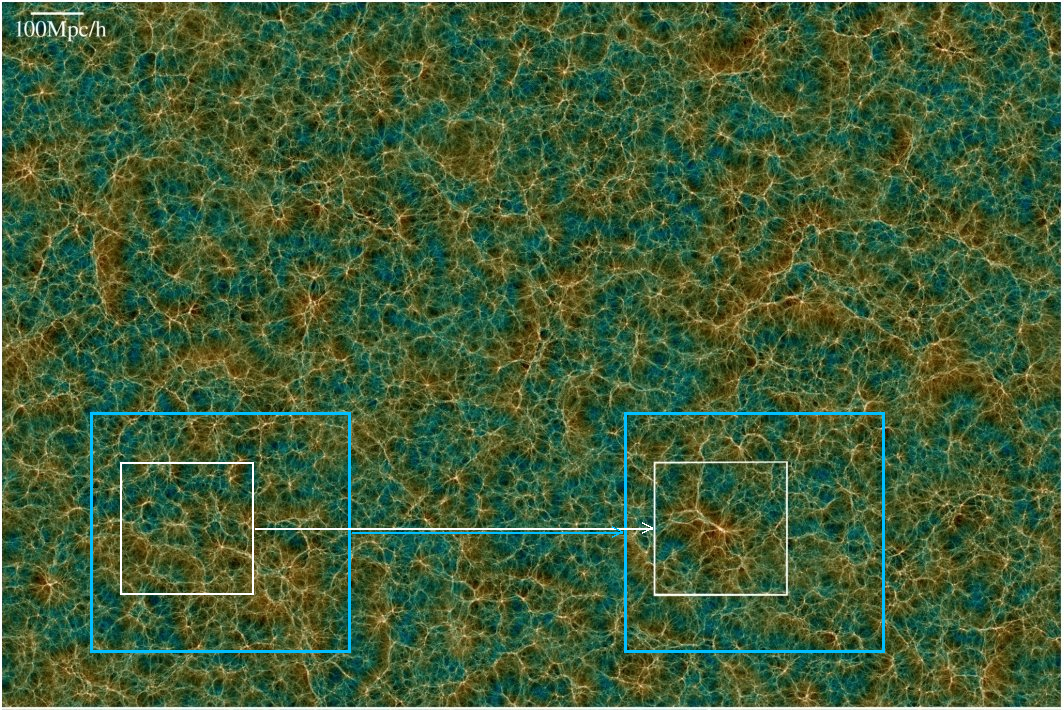
\includegraphics[width=1.0\textwidth]{MainLayout/Introduction_chapter/figures/uchuu_big_box_2.png}
    \caption{Uchuu dark matter simulation of a box $2000 \, \text{Mpc}.h^{-1}$ $\times$ $1333 \, \text{Mpc}.h^{-1}$ with a thickness of $25 \, \text{Mpc}.h^{-1}$. The blue boxes highlight the homogeneity at large scales while the white boxes highlight the inhomogeneity at some scales due to structure formation. Adapted from \cite{Ishiyama_2021}.}
    \label{fig:uchuu_sky}
\end{figure}

\begin{figure}[ht]
    \centering
    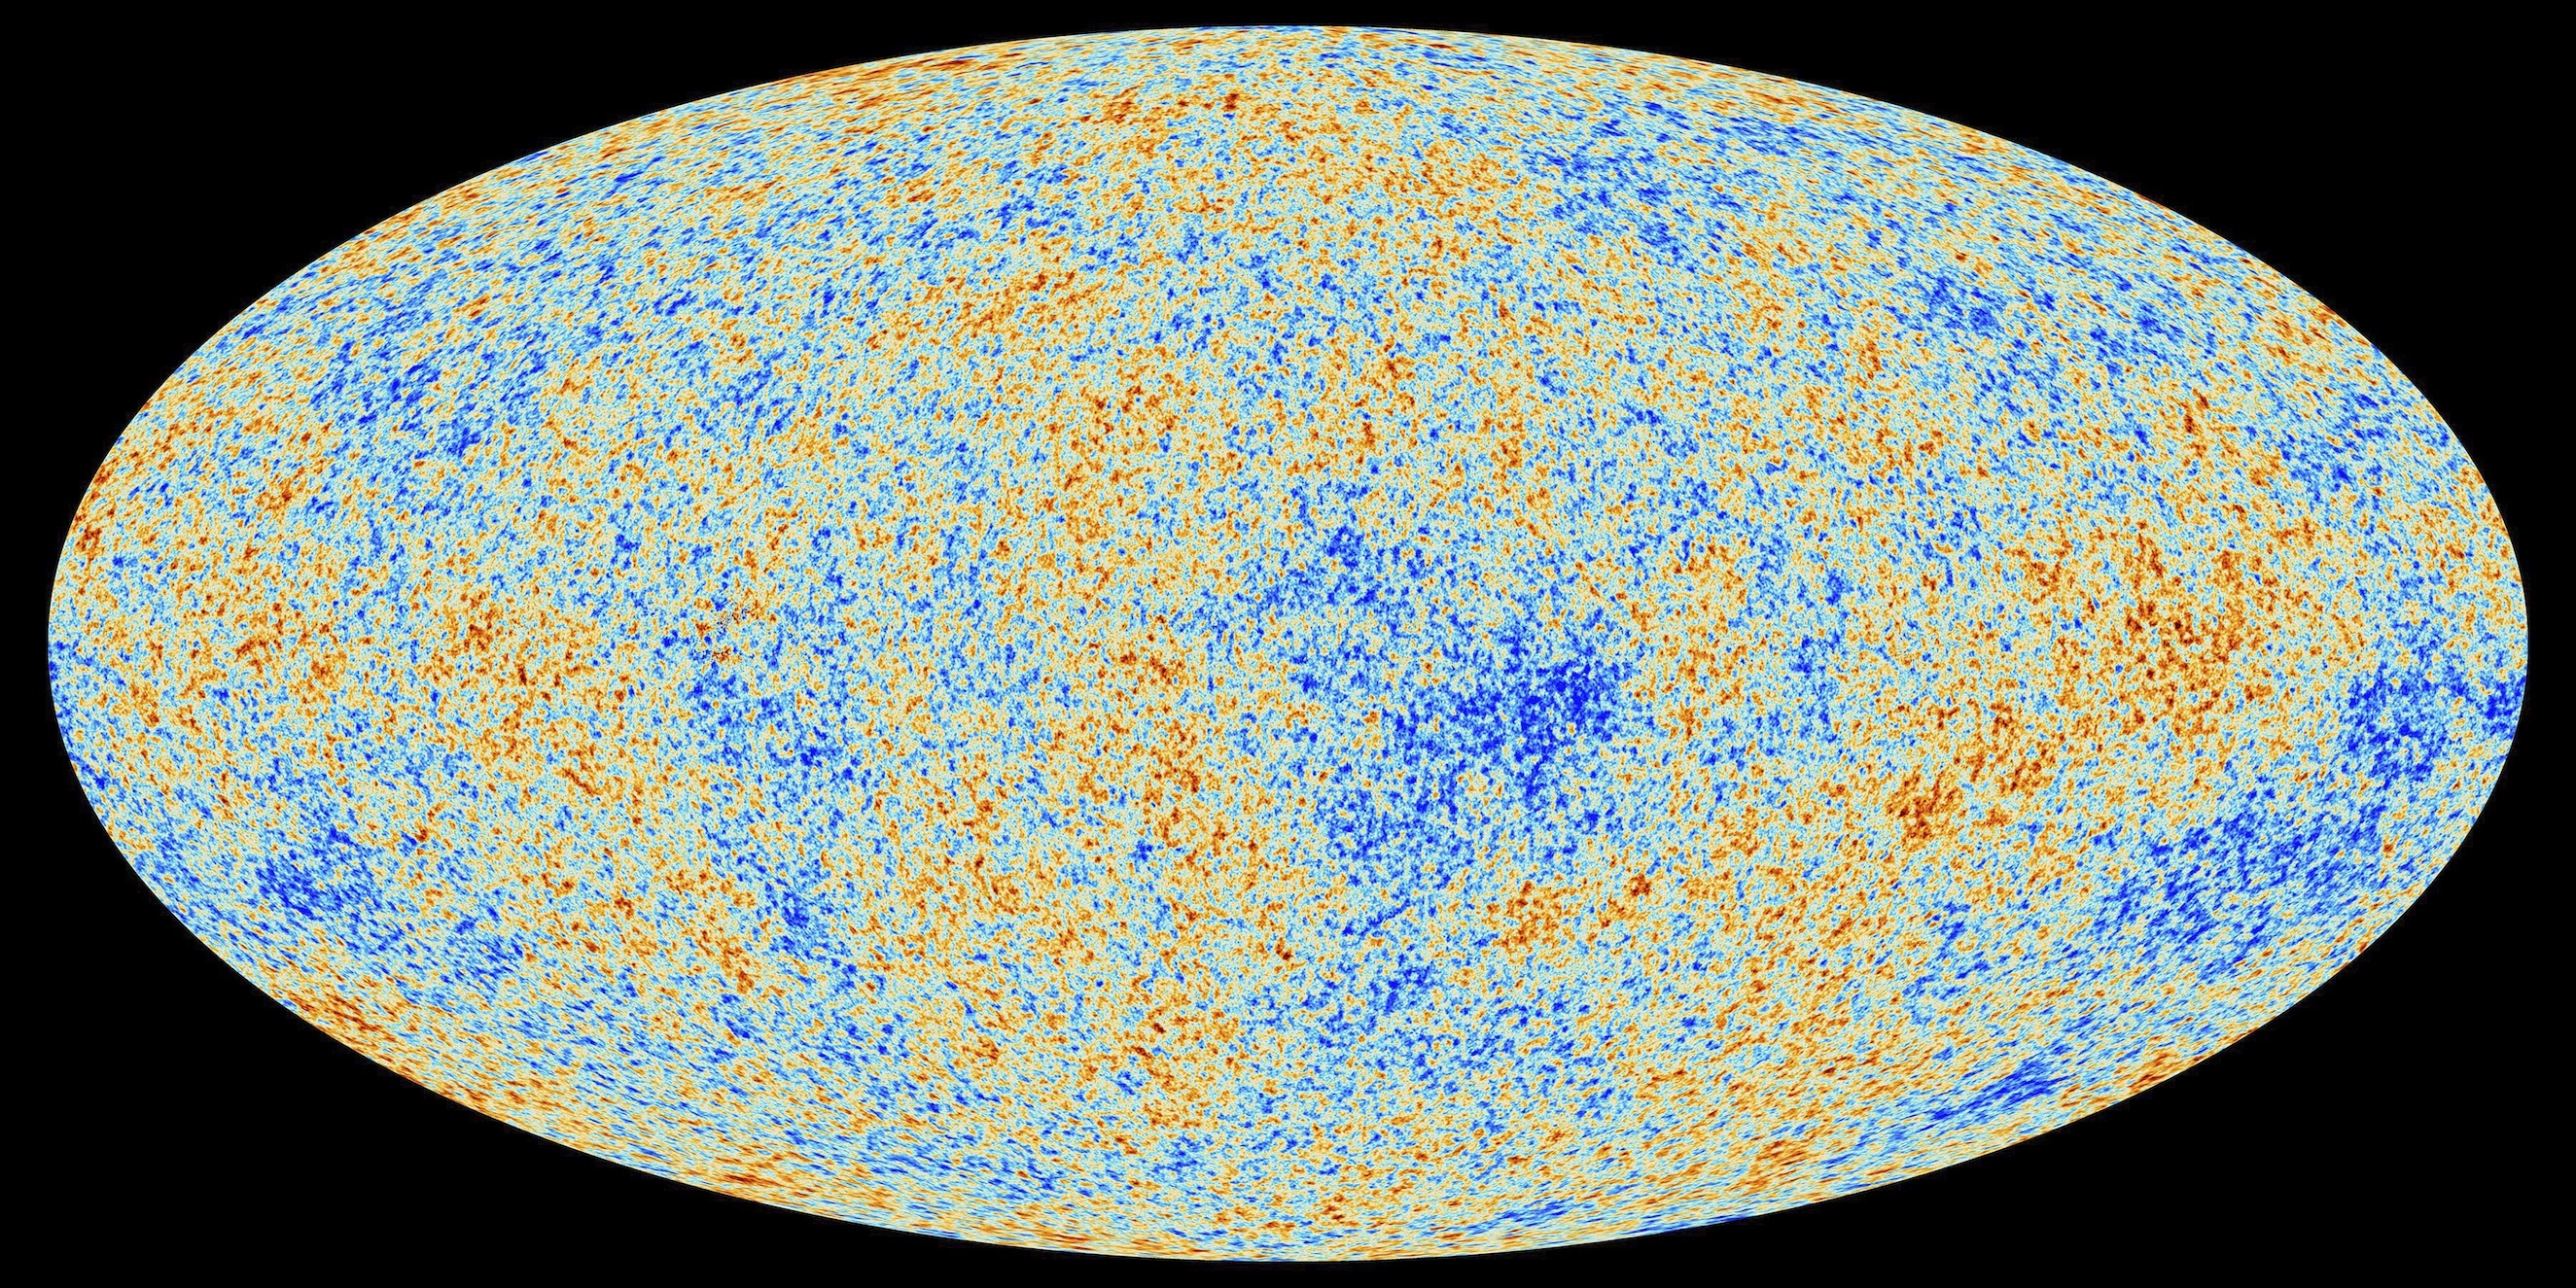
\includegraphics[width=1.0\textwidth]{MainLayout/Introduction_chapter/figures/Cosmic_Microwave_Background_(CMB).jpeg}
    \caption{CMB map provided by ESA and the Planck Collaboration.}
    \label{fig:cmb}
\end{figure}

\noindent \textbf{\underline{Expanding Universe and Hubble relation}} \\

Following the publication of GR, discoveries from \cite{Lemaitre_1927}'s work on the Einstein field equations showed that the proper velocity of a celestial object
was proportional to its distance. Two years later, \cite{Hubble_1929} showed that the radial velocities of 32 nearby galaxies increase with their 
distances indicating an expanding Universe, which is shown in Figure \ref{fig:hubble_og}. The Hubble-Lemaître relation is established as :
\begin{equation}
    v = H_0 d
\end{equation}
where $v$ is the velocity, $d$ the distance of the object and $H_0$ the Hubble constant. Initially, $H_0$ was measured to be around $500 \, \text{km}s^{-1}.\text{Mpc}^{-1}$, 
today more precise measurements show that it is around $70 \,\text{km}s^{-1}.\text{Mpc}^{-1}$. We may also define a \textit{Hubble diagram} as the diagram that relates 
the distance of celestial objects from an observer to their velocities. \\

An expanding Universe entails that objects emitting any kind of waves will be stretched in space making their wavelengths longer. We can call this the \textbf{cosmological 
redshift} $z$ and it is defined as :
\begin{equation}
    1+z = \frac{\nu_{rest}}{\nu_{obs}} = \frac{\lambda_{obs}}{\lambda_{rest}}
\end{equation}
where $\nu_{rest}$ and $\lambda_{rest}$ are the frequency and wavelength emitted at rest-frame and $\nu_{obs}$ and $\lambda_{obs}$ are the observed ones. A source that can affect 
the cosmological redshift is the peculiar velocity of the celestial object which can shift the emitted colour to either bluer or redder frequencies (see Section \ref{sec:vp_methods} where we explain the analysis done with peculiar velocities). \\

\begin{figure}[ht]
    \centering
    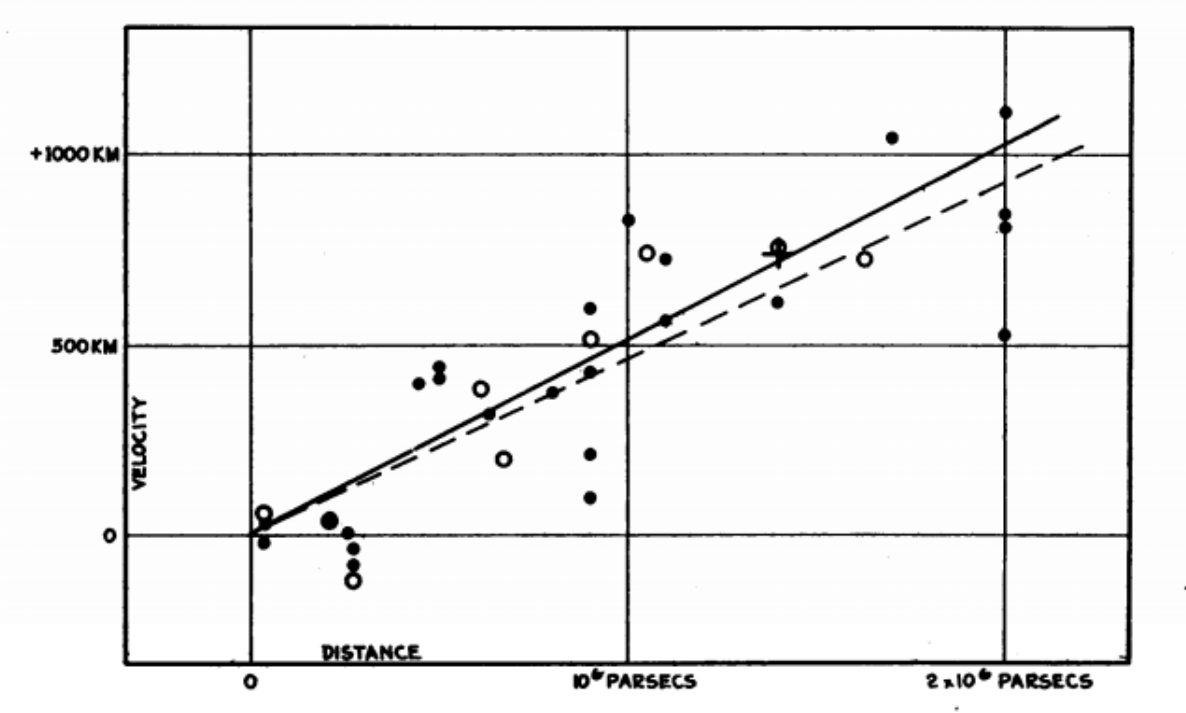
\includegraphics[width=0.8\textwidth]{MainLayout/Introduction_chapter/figures/hubble_og.png}
    \caption{Original Hubble diagram (\cite{Hubble_1929}) portraying the distance velocity diagram of nearby galaxies.}
    \label{fig:hubble_og}
\end{figure}

\subsection{Friedmann-Lemaitre-Robertson-Walker Metric}

We present here a metric that satisfies the homogeneity and isotropy of the Universe as well as an expanding one called Friedmann-Lemaître-Robertson-Walker (FLRW). It is more convenient 
to express the metric in spherical coordinates $(t, r, \phi, \theta)$. Working in natural units $c=1$, we obtain:
\begin{equation}
    ds^2 = dt^2 - a^2(t)\left[ \frac{dr^2}{1-kr^2} + r^2(d\theta^2 + \sin^2(\theta)d\phi^2) \right]
\end{equation}
where $a(t)$ is a dimensionless parameter called the "scale" factor, defined such that today at $t_0$ it is equal to 1, and used to describe the expansion which can be written as :

\begin{equation}
    H(t) = \frac{\dot{a}(t)}{a(t)}
\end{equation}
where the dot denotes the derivative with respect to time and $H(t)$ the Hubble parameter. 
$k$ is a global curvature term such that it can take one of three values $0,-1,1$ to describe a Universe that is flat, open/hyperbolic or closed/spherical respectively.
It is important to note that we can obtain the redshift of an object that emitted a wave at a time $t_e$ from the scale factor as the following relation holds true:
\begin{equation}
    \frac{a(t_0)}{a(t_e)} = 1+z
\end{equation}
Often we apply a change of coordinates such that any object maintains its coordinates regardless of the expansion. These are called comoving coordinates. We define the 
comoving distance $\chi$ such that:
\begin{equation}
    r = S_k(\chi) = \begin{cases}
        S_0(\chi) = \chi \\
        S_{1}(\chi) = \sin(\chi) \\
        S_{-1}(\chi) = \sinh(\chi)
    \end{cases}
\end{equation}
\begin{equation}
    d\chi = \frac{dr}{\sqrt{1-kr^2}}
\end{equation}

The metric then becomes : 
\begin{equation}
    ds^2 = dt^2 - a^2(t)\left[ d\chi^2 + S_k^2(\chi) (d\theta^2 + \sin^2(\theta)d\phi^2) \right]
\end{equation}

\subsection{Friedmann Equations}

Since the Universe is assumed to be homogeneous and isotropic, we can express the energy-momentum tensor $T^{\mu \nu}$ only as a time-dependent object describing the density $\rho$ and pressure 
$P$ of all components present in the Universe. We assume that these can be described as a perfect fluid with no viscosity. For each fluid present indexed by $i$, we can then write down the pressure 
term as $P_i=w_i\rho_i c^2$ where $w$ is the equation of state parameter. This gives us the following form for $T^{\mu \nu}$:
\begin{equation}
    T^{\mu \nu}_i = \rho_i \left[ (w_i+1)u^{\mu}u^{\nu} + w_ig^{\mu \nu} \right]
    \label{eqn:T_mu_nu}
\end{equation}
with $u^{\mu}$ being the velocity vector of the fluid. The local conservation of energy and momentum is expressed by $\nabla_{\mu} T^{\mu \nu} =0 $ where $\nabla_{\mu}$ is the covariant derivative. \\

Using this, the Einstein equations and the FLRW metric, Friedmann derived the following equations known as the Friedmann equations in 1924 (\cite{Friedmann_1922, Friedmann_1924}): 

\begin{equation}
    H^2 = \left( \frac{\dot{a}}{a} \right)^2 = \sum_i \frac{8 \pi G}{3}\rho_i - \frac{kc^2}{a^2}
    \label{eqn:friedmann_1}
\end{equation}
\begin{equation}
    \frac{\ddot{a}}{a} = - \sum_i\frac{4\pi G}{3}\left(\rho_i + 3 \frac{P_i}{c^2}\right)
    \label{eqn:friedmann_2}
\end{equation}

The first equation describes how fast the Universe is expanding knowing the Universe's composition $\rho_i$ and curvature $k$, while the second describes its acceleration.
Combining equations \ref{eqn:friedmann_1} and \ref{eqn:friedmann_2} we get:

\begin{equation}
    \frac{\dot{\rho_i}}{\rho_i} = -3(w_i+1)\frac{\dot{a}}{a}
\end{equation}

And the solution to this differential equation is:

\begin{equation}
    \boxed{\rho_i(t) = \rho_i(t_0)a(t)^{-3(w_i+1)}}
\end{equation}

This entails that the evolution of the scale factor is entirely determined by the nature of the fluids present at a time $t$. Knowing $w$ of each fluid informs us on the behaviour of 
$a(t)$. If we consider one fluid that dominates, the scale factor can be written as:
\begin{equation}
    a(t) \sim t^{\frac{2}{3(1+w)}}
\end{equation}

Consequently, the value of $w$ of the dominant fluid determines the behaviour of the expansion:
\begin{equation}
    \begin{array}{lll}
    \ddot{a}>0 & w<-1/3 & \text{accelerated expansion} \\
    \ddot{a}=0 & w=-1/3 & \text{constant expansion} \\
    \ddot{a}<0 & w>-1/3 & \text{decelerated expansion}
    \end{array}
    \end{equation}

\subsection{Energy Contents of the Universe}

Within the current cosmological framework, the total energy density of the Universe is commonly divided into the following main components:
\begin{itemize}
    \item \textbf{Radiation} ($w_r = \frac{1}{3}$): a relativistic component composed primarily of photons and neutrinos. Its contribution is negligible in the present-day Universe, 
    but it dominated the energy budget during the earliest cosmological epochs.

    \item \textbf{Matter} ($w_m = 0$): a non-relativistic component including both baryonic matter and dark matter. While baryonic matter constitutes the visible content of galaxies, 
    the dominant fraction is dark matter, whose existence was first inferred from galaxy cluster dynamics by Zwicky (\cite{zwicky1933}, \cite{andernach2017}). In the standard cosmological model, dark matter is assumed to be cold, meaning that its particles were non-relativistic during the epoch of structure formation.

    \item \textbf{Cosmological constant / Dark energy} ($w_{\Lambda} = -1$): in the standard $\Lambda$CDM model, cosmic acceleration is described by the cosmological constant $\Lambda$, 
    interpreted as an intrinsic property of spacetime with equation of state $w=-1$. More generally, dark energy may be viewed as an additional fluid component 
    driving accelerated expansion. Possible deviations from $\Lambda$CDM include models with a constant but free equation of state ($w$CDM), or a time-evolving 
    equation of state such as the CPL parametrization (\cite{Chevallier_2001}).
\end{itemize}
\textcolor{red}{COMMENT : might be woth mentioning the quantum vacuum fluctuations and the order of magnitude issue}

The equations of state for matter and radiation can be determined using a statistical physics framework. 
For simplicity, we will not be going into the details of the derivations for each component but simply give the end 
results. \\
\noindent For non-relativistic species, such as matter, we obtain :
\begin{equation}
    w_m = 0
\end{equation}
\noindent For relativistic species, such as radiation, we obtain :
\begin{equation}
    w_r = \frac{1}{3}
\end{equation}

\noindent For the cosmological constant this can be determined without going through the statistical physics. 
Instead, it follows directly from General Relativity by interpreting the cosmological constant as an effective perfect fluid. 
Einstein's field equations can be written as:

\begin{equation}
    G_{\mu\nu}
    =
    \frac{8\pi G}{c^4}
    \left(
    T_{\mu\nu}
    +
    T_{\mu\nu}^{(\Lambda)}
    \right),
\end{equation}
where
\begin{equation}
    T_{\mu\nu}^{(\Lambda)}
    =
    -\frac{\Lambda c^4}{8\pi G}g_{\mu\nu}.
\end{equation}

\noindent Comparing this expression with the stress-energy tensor of a perfect fluid at rest-frame (Equation \ref{eqn:T_mu_nu} where $u^{\mu} = (c,0,0,0)$) 
shows that the cosmological constant behaves as a fluid with energy density:
\begin{equation}
    \rho_{\Lambda}
    =
    \frac{\Lambda c^2}{8\pi G},
\end{equation}
\noindent which is constant by construction since $\Lambda$ is assumed to be constant. Following the energy-momentum conservation we get:
\begin{equation}
    \dot{\rho}
    +
    3H\left(\rho+\frac{P}{c^2}\right)
    =
    0,
\end{equation}
\noindent which then implies:
\begin{equation}
    P_{\Lambda}
    =
    -\rho_{\Lambda}c^2,
\end{equation}
\noindent from which $w_{\Lambda}$ immediately follows,
\begin{equation}
    w_{\Lambda}
    =
    \frac{P_{\Lambda}}{\rho_{\Lambda}c^2}
    =
    -1.
\end{equation}

We introduce the critical density $\rho_c$ defined as the energy density of the Universe for $k=0$ and at $t=t_0$:
\begin{equation}
    \rho_{c,0} = \frac{3H_0^2}{8\pi G}
\end{equation}
This critical density is used to normalize the densities of the other fluids such that the normalized density is written as:
\begin{equation}
    \Omega_{i,0} = \frac{\rho_i(t_0)}{\rho_c}
\end{equation}
At $t=t_0$, the Friedmann equation yields $\Omega_{m,0} + \Omega_{r,0} + \Omega_{\Lambda,0} + \Omega_{k,0} = 1$ with $\Omega_{k,0}$ being the contribution from the curvature by construction at $t=t_0$:
\begin{equation}
    \Omega_{k,t_0} = \frac{-kc^2}{a(t_0)^2H_0^2}
\end{equation}
Equation \ref{eqn:friedmann_1} can be then rewritten as :
\begin{eqnarray}
    H(t) = H_0 \sqrt{ \Omega_{m,0} a(t)^{-3} + \Omega_{r,0} a(t)^{-4} +\Omega_{\Lambda,0} +\Omega_{k,0} a(t)^{-2}}
\end{eqnarray}


Current cosmological observations indicate that the present-day Universe is remarkably close to spatial flatness, corresponding to $\Omega_{k,0}\simeq 0$ 
\cite{Planck_2018_params}. The dominant contribution to the total energy budget is consistent with a cosmological constant (or dark energy), representing 
approximately $70\%$ of the total density. Matter contributes roughly $30\%$, of which about $25\%$ corresponds to dark matter and only $\sim5\%$ to baryonic matter. 
The radiation component today is subdominant, contributing less than $1\%$ of the total energy density. \\

The relative importance of these components evolves with cosmic expansion according to their different scalings with the scale factor. The evolution of 
each energy component is represented in Figure \ref{fig:omega_vs_a}. Since radiation 
scales as $a^{-4}$, matter as $a^{-3}$, and the cosmological constant remains constant, the early Universe was initially radiation dominated. As the Universe 
expanded and cooled, a transition to matter domination occurred, enabling the growth of gravitational instabilities and the formation of large-scale structure. 
At late times, the cosmological constant became dominant, driving the current phase of accelerated expansion. \\

\begin{figure}[ht]
    \centering
    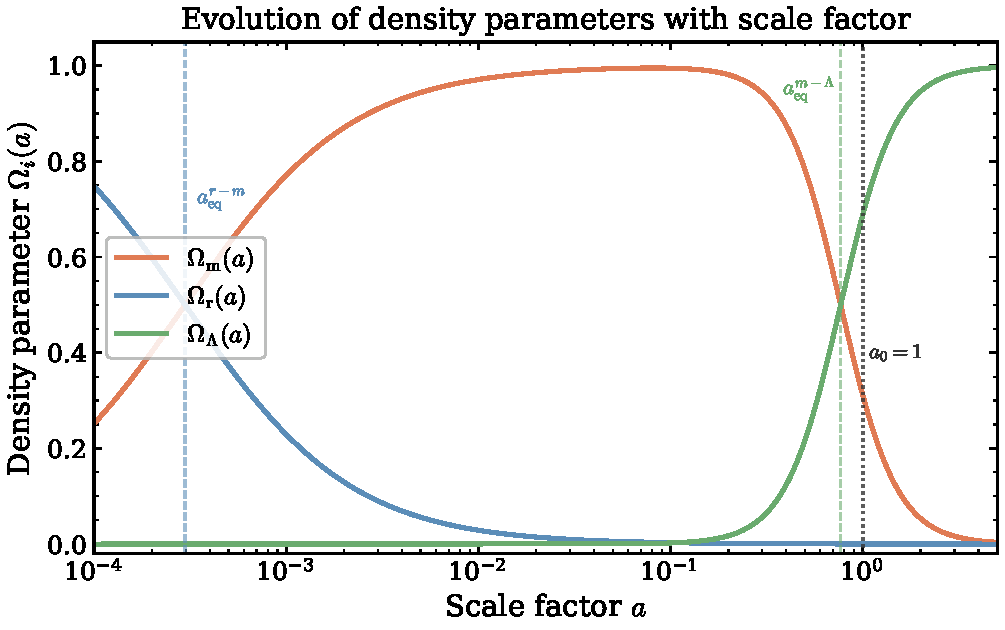
\includegraphics[width=1.0\textwidth]{MainLayout/Introduction_chapter/figures/omega_vs_a.pdf}
    \caption{Evolution of the main components of the $\Lambda$CDM model with respect to the scale factor. This highlights where each component dominates as well as when they become equal.}
    \label{fig:omega_vs_a}
\end{figure}


The acceleration of the Universe was confirmed by \cite{Riess_1998} and \cite{Perlmutter_1999} when they constructed a Hubble diagram with distant Type Ia supernovae. 
Each paper has shown that the supernova Hubble diagram cannot be solely explained with a Universe containing only matter and that an additional energy component must 
be accounted for. This is seen in Figure \ref{fig:hubble_riess}.\\


\begin{figure}[ht]
    \centering
    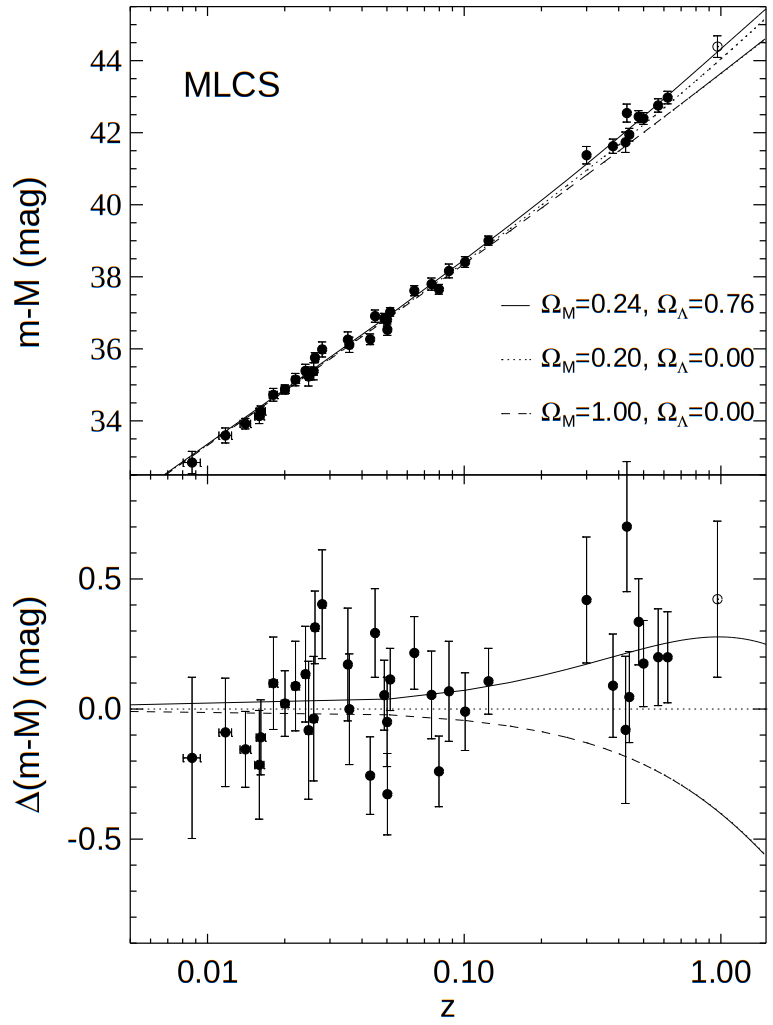
\includegraphics[width=0.7\textwidth]{MainLayout/Introduction_chapter/figures/hubble_riess_.png}
    \caption{Hubble diagram constructed using 50 Type Ia supernovae from \cite{Riess_1998} 
    along the predictions from three Universe models containing: only matter (20\% of the energy content) as a dotted line; 
    only matter (100\% of the energy content) as a dashed line; and matter (24\%) + $\Lambda$ (76\%) as a solid line. The data fits the solid line best.}
    \label{fig:hubble_riess}
\end{figure}

\subsection{The $\Lambda$CDM Model}

The $\Lambda$CDM model is the standard model of cosmology. It is built upon the framework of GR and assumes that the Universe began in an 
extremely hot and dense state, known as the Hot Big Bang, and has been expanding ever since. As the Universe expanded and cooled, it underwent three 
successive epochs of domination by different energy components, each governing the dynamics of expansion through the Friedmann equations: a radiation 
dominated era at early times, followed by a matter dominated era, and finally the current dark energy dominated era driven by the cosmological 
constant $\Lambda$. \\

The energy content of the Universe in $\Lambda$CDM consists of the components introduced in the previous section: radiation, baryonic matter, cold dark matter 
and a cosmological constant $\Lambda$, with their present-day fractions measured to be approximately $\Omega_r \approx 9 \times 10^{-5}$, $\Omega_b \approx 0.05$, 
$\Omega_{\text{CDM}} \approx 0.26$ and $\Omega_\Lambda \approx 0.69$ respectively 
(\cite{Planck_2018_params}), in a spatially flat Universe where $\sum_i \Omega_i = 1$. The model makes the additional assumptions that the 
Universe is homogeneous and isotropic on large scales (the cosmological principle), and that the primordial density perturbations seeding all structures are adiabatic 
and nearly Gaussian (\cite{Planck_2018}). \\

The $\Lambda$CDM model is fully characterised by six independent cosmological 
parameters:

\begin{itemize}
    \item $A_s$ — the amplitude of primordial scalar perturbations
    \item $n_s$ — the spectral index of the primordial power spectrum
    \item $\Omega_b h^2$ — the physical baryon density
    \item $\Omega_{\text{CDM}} h^2$ — the physical cold dark matter density
    \item $\theta_*$ — angular size of the sound horizon at recombination 
    \item $\tau$ — the optical depth to reionization
\end{itemize}

All other cosmological quantities, such as $\Omega_\Lambda$, $\sigma_8$ and $S_8$, are derived from these six parameters within the model. 
For example, $\sigma_8$ can be related to $A_s$ such that:
\begin{equation}
    \sigma_8 \propto \sqrt{A_s}
\end{equation}
Despite its simplicity, $\Lambda$CDM has proven remarkably successful in describing a wide range of observations, from the CMB anisotropies (\cite{Planck_2018_params}) to the 
large-scale distribution of galaxies (\cite{DESI_DR2_2025}), the BAO standard ruler 
(\cite{Eisenstein_2005}), and the accelerated expansion of the Universe (\cite{Riess_1998, Perlmutter_1999}). Nevertheless, as discussed in Section 
\ref{sec:tensions}, emerging tensions between different observational probes suggest that $\Lambda$CDM may require extensions or modifications.\\

The $\Lambda$CDM model is founded on the Hot Big Bang paradigm, whose success rests on three major observational pillars. These pillars are:
\begin{itemize}
    \item Expansion of the Universe as observed by Hubble in \cite{Hubble_1929}.
    \item Big Bang Nucleosynthesis (BBN) which predicts the primordial abundances of light elements (hydrogen, helium, and lithium) formed at the very early stages of the Universe (\cite{Cyburt_2016}, \cite{Wagoner_1967}).
    \item Cosmic Microwave Background (CMB), the trace of thermal radiation released when the Universe cooled sufficiently for protons 
    and electrons to recombine into neutral hydrogen at $z \sim 1100$ (\cite{Penzias_1965_a}, \cite{Penzias_1965_b}) (more details in Section \ref{section:cmb}). 
\end{itemize}
Together, these three pillars provide strong evidence for a hot, dense early Universe that has been expanding and cooling ever since. \\


Although $\Lambda$CDM describes the Universe as homogeneous and isotropic at the largest scales, this description breaks down at smaller scales where 
structures such as galaxies and galaxy clusters emerge. Explaining the emergence of inhomogeneous structures from an initially homogeneous Universe, while preserving the 
assumptions of $\Lambda$CDM, is an important challenge. We describe this process in the following section. \\
\section{Large Scale Structure Formation}

Now that we have understood how modern cosmology came to be, we can move on to understanding the formation of structures. Observations from galaxy surveys such as DESI show that 
although on large scales the Universe looks homogenous, the smaller scales indicate the existence of an underlying non-homogenous structure. This can be seen through the formation of galaxy clusters 
and the cosmic web. Understanding how these structures are formed gives us a lot of information regarding the strength of gravity at large scales as well as the amount of matter in the Universe.
Since the full derivation of each equation in structure formation is too long to write for this thesis, we recommend reading \cite{Knobel_2013} and \cite{Dodelson_2003} for a more detailed derivation\\


\subsection{Newtonian approach to structure formation}

In this introductory section, we will be starting off by describing structure formation by going only to linear scales. This will be the model on which we build up more complex 
structure formation model. \\

\noindent \textbf{\underline{Theory of structure formation}} \\

We start by assuming a Universe is filled with an inhomogeneous, dissipationless, ideal fluid with matter density $\rho(\mathbf{r},t)$, velocity field $\vec{v}(\mathbf{r}, t)$, 
pressure $P(\mathbf{r},t)$ and entropy per unit mass $S(\mathbf{r}, t)$ with $\mathbf{r}$ being the fluid's coordinates. We obtain the following hydrodynamical equations:
\begin{equation}
    \begin{cases}
        \frac{\partial \rho}{\partial t} + \vec{\nabla}. (\rho \vec{v}) = 0 & \mathrm{Continuity\; equation\;} \\
        \frac{\partial \vec{v}}{\partial t} + (\vec{v} . \vec{\nabla}) \vec{v} + \frac{\vec{\nabla} P }{\rho} + \vec{\nabla}\Phi = 0 & \mathrm{Euler\; equation\;} \\
        \nabla^2 \Phi = 4 \pi G \rho & \mathrm{Poisson\; equation\;} \\
        \frac{\partial S}{\partial t } + (\vec{v} . \vec{\nabla}) S = 0& \mathrm{Entropy\; conservation\;}
    \end{cases}
    \label{eqn:hydro_eqn}
\end{equation}
with $\Phi$ the gravitational potential. Since matter is approximated as a single-stream fluid, 
neighboring particles follow nearly parallel trajectories without "shell crossing" (collision of streams). This description breaks down once nonlinear collapse occurs, 
when multiple streams overlap and complex dynamics emerge. A fully accurate treatment of structure formation would instead 
require solving the general relativistic Boltzmann equation including all cosmic components and their interactions, although this is in itself a difficult problem due to the nonlinear 
coupling between the fluid equations. To overcome that issue, we assume a FLRW Universe and perturb the fluid around the Hubble flow, meaning we 
separate each variable as a homogenous part and an inhomogeneous perturbation:
\begin{align*} 
    \rho(\mathbf{r},t) &=  \bar{\rho}(t) + \delta \rho(\mathbf{r},t) \\ 
    \mathbf{v}(\mathbf{r},t) &=  \bar{\mathbf{v}}(\mathbf{r},t) + \delta \mathbf{v}(\mathbf{r},t) \\
    P(\mathbf{r},t) &=  \bar{P}(t) + \delta P(\mathbf{r},t) \\
    \Phi(\mathbf{r},t) &=  \bar{\Phi}(\mathbf{r},t) + \delta \Phi(\mathbf{r},t) \\
    S(\mathbf{r},t) &=  \bar{S}(t) + \delta S(\mathbf{r},t) \\
\end{align*}
\textcolor{red}{COMMENT : detail why not relativistic treatment and small perturbations}

We can then re-introduce our new variables in Equations \ref{eqn:hydro_eqn} although to slightly simplify the equations we will be working in comoving coordinates $\mathbf{x}$ such that 
\begin{align*}
    \mathbf{r} = a \mathbf{x} \\
    \nabla_{\mathbf{r}} = \frac{1}{a} \nabla_{\mathbf{x}} \\
    \frac{\partial}{\partial t}\bigg\rvert_{\mathbf{r}} = \frac{\partial}{\partial t}\bigg\rvert_{\mathbf{x}} - \frac{1}{a}\mathbf{v} . \nabla_{\mathbf{x}} \\
\end{align*}
We will also be working in Fourrier space where we get for any perturbation $\delta q(\mathbf{x}, t)$:
\begin{equation}
    \delta q(t, \mathbf{k}) = \int \delta q (t, \mathbf{x}) e^{-i \mathbf{k}\mathbf{x}} \mathrm{d}^3x
\end{equation}

\begin{equation}
    \delta q(t, \mathbf{x}) = \frac{1}{(2\pi)^3} \int \delta q (t, \mathbf{k}) e^{-i \mathbf{k}\mathbf{x}} \mathrm{d}^3k
\end{equation}
With $\mathbf{k}$ are the comoving Fourrier modes. We get the following hydrodynamical equations at first order:
\begin{equation}
    \boxed{
    \begin{cases}
        \delta \dot{\rho} + 3H\delta \rho + \frac{i\bar{\rho}\mathbf{k}}{a} . \delta\mathbf{v} = 0& \mathrm{Continuity\; equation\;} \\
        \delta \dot{\mathbf{v}} + H \delta \mathbf{v} + \frac{i\mathbf{k}}{a\bar{\rho}}(c_s^2 \delta \rho + \sigma \delta S) + \frac{i \mathbf{k}}{a} \delta \Phi = 0 & \mathrm{Euler\; equation\;} \\
        k^2 \delta \Phi + 4 \pi G a^2 \delta \rho = 0 & \mathrm{Poisson\; equation\;} \\
        \delta \dot{S} = 0& \mathrm{Entropy\; conservation\;}
    \end{cases}
    }
    \label{eqn:newton_hydro_eqn}
\end{equation}
with $c_s^2 = (\partial \bar{P}/ \partial \bar{\rho})_{\bar{S}}$ the speed of sound in the fluid, $\sigma = (\partial \bar{P}/ \partial \bar{S})_{\bar{\rho}}$ and $k=|\mathbf{k}|$. \\

\textcolor{red}{COMMENT : how do we get the 3h delta rho?} \\


What we are interested in is essentially how do matter perturbation grows as they will give birth to structure by gravitational attraction. The first thing to note is 
that the entropy fluctuations must exist at early times in order for them to keep existing otherwise they would simply dissipate. Moreover, results from the simplest 
models of inflation do not support the fluctuations of entropy. So from now on we well set $\delta S = 0$. We can also assume that the velocity perturbations would follow the overdense regions giving us 
$\mathbf{k} || \delta \mathbf{v}$. We call the modes that result from these conditions the adiabatic modes. \\
\textcolor{red}{COMMENT : say no vorticity to justify parallel and separate from adiabatic modes}.

We will be denoting the overdensity $\delta(\mathbf{k},t)$ as the matter density contrast which is written as:
\begin{equation}
    \delta(\mathbf{k}, t) = \frac{\rho(\mathbf{k},t)}{\bar{\rho}(t)} - 1 = \frac{\delta \rho (\mathbf{k}, t)}{\bar{\rho}(t)}
\end{equation}

In the adiabatic modes, the continuity equation becomes:
\begin{equation}
    \dot{\delta} + \frac{ik}{a}\delta v = 0
\end{equation}
If we then differentiate this equation and combining its results with Euler and Poisson equations we obtain:
\begin{equation}
    \ddot{\delta} + 2 H \dot{\delta} + \left( \frac{c_s^2 k^2}{a^2} - 4\pi G \bar{\rho} \right)\delta = 0
    \label{eqn:linear_dens}
\end{equation}
Here we obtain a linear second order differential equation with two solutions to it. We denote $\lambda = \frac{2\pi a}{k}$ the physical wavelength of the mode, 
$\lambda_J = c_s \sqrt{\frac{\pi}{G\rho}} $ the Jeans length and $M_J = \frac{\pi}{6} \lambda_J^3 \bar{\rho} $ the Jeans mass. Equation \ref{eqn:linear_dens} tells us that 
if $\lambda < \lambda_J$, the solution to the equation is an oscillating wave leaving no room for structures to grow. So a condition we must have is $\lambda > \lambda_J$. We 
place ourselves in the condition where the wavelength is much larger than the Jeans length $\lambda \gg \lambda_J$, Equation \ref{eqn:linear_dens} is now reduced to:
\begin{equation}
    \ddot{\delta} + 2 H \dot{\delta} - 4\pi G \bar{\rho} \delta = 0
\end{equation}

\textcolor{red}{COMMENT : important to specify this reduction for collisionless matter so DM but not baryonic} \\


which has the following general solution:
\begin{equation}
    \delta(\mathbf{k},t) = \delta_+(\mathbf{k})D_+(t) + \delta_-(\mathbf{k})D_-(t)
\end{equation}
with the + and - denoting growing and decaying modes. We call the $D_+(t)$ term the \textbf{linear growth function}. In the radiation dominated era, the Mészáros 
effect suppresses the growth of sub-Hubble matter perturbations, which grow only logarithmically rather than as a power law. In the matter dominated era 
the expansion rate grows as $H(t) = \frac{2}{3t}$ which gives us:
\begin{equation}
    \boxed{D_+ \propto t^{2/3} \propto a(t)}
\end{equation}
\begin{equation}
    D_- \propto t^{-1}
\end{equation}
This means that we can get grown modes for matter perturbations in the matter dominated era with $D_+$ while $D_-$ goes to 0. A general formula for $D_+$ can be obtained 
(\cite{Carroll_1992}) and it gives us:
\begin{equation}
    D_+(z) = \frac{1}{1+z} \frac{g(z)}{g(0)}
\end{equation}
\begin{equation}
    g(z) = \frac{\Omega_m(z)}{\Omega^{4/7}_m(z)-\Omega_{\Lambda}(z) + (1+\Omega_m(z)/2)(1+\Omega_{\Lambda}(z)/70)}
\end{equation}

The growth of perturbations described by $D_+$ can be characterised by the \textit{growth rate} $f$, defined as the logarithmic derivative of the growth factor 
with respect to the scale factor:
\begin{equation}
    f = \frac{d \ln D_+}{d \ln a}
\end{equation}
In the matter dominated era, since $D_+ \propto a$, we get $f = 1$. A useful approximation valid across different epochs and cosmologies is given by 
(\cite{Peebles_1980}):
\begin{equation}
    \boxed{f \approx \Omega_m(z)^{\gamma}}
\end{equation}
where $\gamma$ is obtained from the underlying gravitational theory. For a flat $\Lambda$CDM cosmology and GR it is $\gamma \simeq 0.55$. 
Deviations from this value would indicate modifications to GR on cosmological scales. 
In practice, $f$ is not directly observable, and is instead measured in combination with $\sigma_8$, the root mean square of matter fluctuations on scales of 
$8 \, h^{-1}$Mpc. The combination $f\sigma_8$ is therefore the key observable quantity that encodes 
the rate of growth of large-scale structure and provides a direct test of gravity on cosmological scales. \\

\textcolor{red}{COMMENT : not just Peebles more ref and there is an expression for gamma wrt w} \\
\textcolor{red}{COMMENT : can relate here or later As conneciton} \\


\noindent \textbf{\underline{Statistical analysis of overdensities}} \\

Practically, we perform a statistical analysis when it comes to the study of the structures of the Universe. $\delta$ is looked at as a realization of a stochastic process 
and by analyzing that we can compare our observations to theories. \\

\textcolor{red}{COMMENT : primordial fluctuations expected from inflation described in later section implies stochastic nature etc... can relate to CMB observations 
today (just to make the link)} \\

We introduce $\langle...\rangle$ as the ensemble average of the stochastic process underlying a random field. The large-scale structure we observe is only one realization 
of an underlying random cosmic process, so estimating its true statistical properties requires additional assumptions. A common assumption is ergodicity, meaning that 
averages measured over a sufficiently large volume of the Universe approximate the averages over many hypothetical realizations. In practice, this is related to the fair 
sample hypothesis, which assumes that widely separated regions of the Universe can be treated as nearly independent samples of the same process. If the survey volume is 
large enough and correlations become weak on large scales, these approximations are reasonable. However, real galaxy surveys cover finite volumes and therefore their measured 
averages are affected by statistical fluctuations known as \textbf{sample variance}, or \textbf{cosmic variance} when limited by the size of the observable Universe.\\

We denote the 2-point correlation function as:
\begin{equation}
    \xi(\mathbf{x}, \mathbf{x}') = \left\langle \delta(\mathbf{x}) \delta(\mathbf{x}') \right\rangle
\end{equation}
Our field is homogenous and isotropic therefore the only 
quantity that affects the correlation function is $r=|\mathbf{x} - \mathbf{x}'|$, $\xi(\mathbf{x}, \mathbf{x}')=\xi(r)$. If at $r=+\inf$, the correlations go to 0, 
then we can decompose it in Fourrier modes:
$\delta(\mathbf{k})$:
\begin{equation}
    \left\langle \delta(\mathbf{k}) \delta^*(\mathbf{k}') \right\rangle = (2 \pi)^3 \delta_D(\mathbf{k} - \mathbf{k}')\mathcal{P}(\mathbf{k})
\end{equation}
\begin{equation}
    \mathcal{P}(\mathbf{k}) = \int \xi(\mathbf{x})e^{-i \mathbf{k} \mathbf{x}} d^3x
\end{equation}
where the $\mathcal{P}(k)$ is the \textbf{power spectrum}, which is a real function, and $\delta_D$ is the Dirac delta function. \\
The works from \cite{Harrison_1970}, \cite{Zeldovich_1970_pk} and \cite{Peebles_1970} show that there is a preferrable form for the initial primordial power spectrum that takes the form:
\begin{equation}
    \mathcal{P}(k) \propto k^{n_s}
\end{equation}
with $n_s$ the \textbf{spectral index}. If $n_s=1$ the power spectrum becomes scale invariant. It is possible to predict the shape of the power spectrum of the initial conditions by studying an inflationary model. Most common models 
and results from \cite{Planck_2018} indicate that the initial perturbations are Gaussian with $n_s \approx 1 $. \\
The power spectrum for the linear overdensity field is:
\begin{equation}
    \mathcal{P}_{\mathrm{lin}}(t, k) = A_s k^{n_s}T^2(k)D^2_+(t)
\end{equation}
with $A_s$ the normalization parameter and $T(k)$ is the transfer function which characterizes how each Fourrier mode of the density field evolved from the initial conditions to 
a later time. \\
\textcolor{red}{COMMENT : can link sigma8 and As here} \\


\subsection{Relativistic structure formation}

Similarly to the previous section, we will be introducing structure formation from a general relativistic framework with a focus on linear perturbation. We will not be deriving 
every single quantity, however explaination of how we get there and how it relates to the Newtonian approximation will be present. \\

\noindent \textbf{\underline{General description of perturbations}} \\

Firstly, we will be working in the FLRW metric for $k=0$. We will also work in conformal time $\tau$ which simplifies this problem. 
It is defined as $a \mathrm{d}\tau = \mathrm{d}t$. We will also work in natural units setting $c=\hbar =1$. We will denote the FLRW metric as $\bar{g}_{\mu \nu}$ so that 
for a flat spacetime we have:
\begin{equation}
    ds^2 = \bar{g}_{\mu \nu} dx^{\mu} dx^{\nu} = a^2(\tau)\left( - d\tau^2 + \bar{\gamma}_{ij} dx^{i} dx^{j} \right)
\end{equation}
where $\bar{\gamma}_{ij}$ is the metric for the spatial components and $(i,j)$ can take the values $1,2,3$ (in general we will put a bar on top of the parameter related to a flat FLRW metric). \\

In a relativistic framework, the perturbations are done on the metric in itself such that when we choose a metric $g_{\mu \nu}$ the deviations from the homogenous isotropic 
background are close enough to $\bar{g}_{\mu \nu}$\footnote{Mathematically, this change in metric means we alsothe mainifolds being worked on so simple mathematical operations
no longer apply. One way to overcome that issue is to define $\bar{g}_{\mu \nu}$'s functional form as invariant under coordinate transformations.}. We then obtain:
\begin{equation}
    \delta g_{\mu \nu} = g_{\mu \nu}(x) - \bar{g}_{\mu \nu}(x)
\end{equation} 
Physically, we are splitting $g_{\mu \nu}$ into a background $\bar{g}_{\mu \nu}$ and perturbation $ \delta g_{\mu \nu}$. However this perturbation is not a 4-tensor which will 
require us to set a gauge transformation. Similarly, the perturbation for a general scalar-like object and a vecotr-like objects are defined as:
\begin{equation}
    \delta q(x) = q(x) - \bar{q}(x)
\end{equation}
\begin{equation}
    \delta q^{\mu} = q^{\mu} - \bar{q}^{\mu} = \delta q_{\nu} \bar{g}^{\mu \nu} + \bar{q}_{\nu} \delta g^{\mu \nu}
\end{equation}
We can also perform the same for the energy-momentum tensor.
\begin{equation}
    \delta T_{\mu \nu} = T_{\mu \nu} - \bar{T}_{\mu \nu}
\end{equation}
with 
\begin{equation}
    T_{\mu \nu} = (\rho + P)u_{\mu}u_{\nu} + P g_{\mu \nu} + \Pi_{\mu \nu}
\end{equation}
and $\Pi_{\mu \nu}$ is the anisotropic stress which accounts for deviations from an ideal fluid. \\

The general form for the metric perturbation is written as:
\begin{equation}
    \delta g_{\mu \nu} dx^{\mu} dx^{\nu} = a^2(\tau)\left[ -2A d\tau^2 + B_i d\tau dx^i + 2(H_L \delta_{ij} + H_{ij})dx^i dx^j \right]
\end{equation}
where $A(\tau, \mathbf{x})$, $B_i(\tau, \mathbf{x})$, $H_L(\tau, \mathbf{x})$ and $H_{ij}(\tau, \mathbf{x})$ are perturbation quantities and $\delta_{ij}$ a delta function.\\

\noindent \textbf{\underline{Newtonian gauge}} \\

These perturbation quantities intervene will then intervene in the field equations. Determining them necessitates a gauge transformation. We will be showing the results 
of the Newtonian gauge as it is useful for analyzing the density fluctuations inside of the Hubble horizon ($D_H = 1/H$) as well as it is simple to interpret its results in terms of 
Newtonian physics. The gauge is defined by:
\begin{equation}
    B=H=0
\end{equation}
and we will be renaiming the other perturbations as:
\begin{equation}
    \Psi = A
\end{equation}
\begin{equation}
    \Phi = -H_L
\end{equation}

The field equations for the Newtonian gauge are:
\begin{equation}
    \boxed{
    \begin{cases}
        -k^2 \Phi - 3H(\dot{\Phi} + H\Psi) = 4 \pi G a^2 \delta \rho \\
        \dot{\Phi} + H \Psi = 4 \pi G a^2 \frac{v}{k} (\bar{\rho} + \bar{P}) \\
        \ddot{\Phi} + H(\dot{\Psi} + 2\dot{\Phi}) + (2 \dot{H} + H^2)\Psi + \frac{k^2}{3}(\Phi - \Psi) = 4 \pi G a^2 \delta P \\
        k^2 (\Phi - \Psi) = 8 \pi G a^2 \Pi
    \end{cases}
    }
\end{equation}
where the dots are derivatives with respect to the conformal time. 
If we consider scale much smaller than the Hubble horizon $H/k \ll 1$, the first field equation then becomes:
\begin{equation}
    -k^2 \Phi = 4 \pi G a^2 \delta \rho
\end{equation}
In this limit we recover the Poisson equation in the Newtonian formalism. Therefore, we can say that well within the horizon the Newtonian gauge reduces to Newtonian mechanics. 
This also means we can have a physical interpretation for $\Phi$ it acting as the Newtonian gravitational potential (called generalized Newtonian potential). The last equation 
also informs us that in the matter dominated epoch we have $\Phi \simeq \Psi$ reducing the metric perturbations to only one parameter. \\

One can only also derive the equations of motion in the Newtonian gauge, however for this thesis we will only be showing the final equations of motions obtained for matter 
fluctuations in the matter dominated era. We note the matter overdensity $\delta_m = \frac{\delta \rho_m}{\bar{\rho}}$, we obtain:
\begin{equation}
    \ddot{\delta}_m + H \dot{\delta}_m - 4\pi G a^2 \bar{\rho}_m\delta_m = 0
\end{equation}

\subsection{Inflation}

Inflation is a period of time at the very early stages of the Universe 
where an accelerated expansion of the Universe occurred (\cite{Guth_1981}). It was theorized to tackle known issues regarding the fine tuning of the flatness of the Universe and the horizon problem.
What we see as well is that through inflation we can have a predict for the initial density fluctuations. 
This following condition is imposed on inflation to obtain an accelerated early Universe:
\begin{equation}
    \ddot{a} > 0
\end{equation}

During inflation, we assume that the Universe is dominated by a quantum scalar field $\phi$ called the inflaton, experiencing a "slow roll" down its potential $V(\phi)$ (\cite{Mukhanov_1992}, \cite{Albrecht_1982}). 
The action for a scalar field minimally coupled to gravity is given by:
\begin{equation}
    S = \int d^4x \sqrt{-g} \left[ \frac{M^2_{\mathrm{pl}}}{2} R - \frac{1}{2} g^{\mu \nu} \partial_{\mu}\phi \partial_{\nu}\phi - V(\phi) \right]
\end{equation}
where $M_{\mathrm{pl}} $ is the Planck mass defined as $M^2_{\mathrm{pl}} = \left(\frac{1}{8\pi G}\right)^2$. Varying the action with the respect to the metric allows to obtain 
the energy momentum tensor $T_{\mu \nu}$ and its components $P_{\phi}$ and $\rho_{\phi}$:
\begin{equation}
    P_{\phi} = \frac{1}{2} \dot{\phi}^2 - V(\phi)
\end{equation}
\begin{equation}
    \rho_{\phi} = \frac{1}{2} \dot{\phi}^2 + V(\phi)
\end{equation}
where the kinetic energy of the field is given by $\frac{1}{2} \dot{\phi}^2$.\\
The dynamics can be recovered with the Klein Gordon equation giving us:
\begin{equation}
    \ddot{\phi} + 3H \dot{\phi} + \frac{d V(\phi)}{d \phi} = 0
\end{equation}

We can also apply the Friedmann equations to the inflaton field where we get:
\begin{equation}
    H^2 = \frac{1}{M^2_{\mathrm{pl}}}\left( \frac{1}{2} \dot{\phi}^2 + V(\phi) \right)
\end{equation}
\begin{equation}
    \dot{H} = -\frac{1}{2} \frac{\dot{\phi}^2}{3M^2_{\mathrm{pl}}}
\end{equation}

Assuming a slow rolling field entails that kinetic term is small compared to the potential term $V$. We can show that given this assumption $a \sim e^{Ht}$ which is a necessary
condition to inflation. Additionally we assume coherent oscillations around a minimum that are damped by a $H\dot{\phi}$ as seen in the Klein-Gordon equation. The field is 
then expected to decay into matter and radiation, although the exact physical process behind that is unknown. The 
inflaton field is then treated as a perturbation around a mean field, that these perturbation give rise to perturbation amplitudes that we can identify in the observations we make today. 
Some useful parameters to define for a slow-roll inlfation are :
\begin{equation}
    \epsilon = - \frac{\dot{H}}{H^2} = \frac{3}{2} \frac{\dot{\phi}^2}{V}
\end{equation}
\begin{equation}
    \eta = \epsilon - \frac{\ddot{\phi}}{H \dot{\phi}}
\end{equation}
where the slow rolling conditions are $\epsilon \ll 1$ and $\eta \ll 1$. \\
We define $q$ as:
\begin{equation}
    q(x) = \delta \phi + \frac{\dot{\bar{\phi}}}{H} \Phi
\end{equation}
This quantity $q$ is known as the Mukhanov-Sasaki variable
(\cite{Mukhanov_1988}, \cite{Sasaki_1986}) and is the canonical variable for quantizing inflaton perturbations.\\

In order to fully treat the inflaton field we have to apply the canonical quantization of the field (quantum field theory) by elevating $q$ to an operator $\hat{q}$ as well as introducing 
its canonical conjugate momentum $\hat{\pi}$. In the Fourrier space, they are expressed as function of the quantum harmonic operator $a_{\mathbf{k}}$ and $a_{\mathbf{k}}^{\dag}$. 
With these operators we can calculate the expected value of the field as well as power spectrum as a function of $k$. 
Once the power spectrum during inflation is determined it is possible to extend this to the primordial power spectrum of matter during the matter dominated era. 
Outside the Hubble horizon, each mode is frozen with a nearly scale-invariant amplitude. 
Before writing the primordial power spectrum, we introduce the comoving curvature perturbation $\mathcal{R}$, a gauge-invariant 
quantity that measures the spatial curvature of constant-density hypersurfaces. In the context of inflation it is related to the inflaton perturbation $\delta\phi$ by:
\begin{equation}
    \mathcal{R} = -\frac{H}{\dot{\bar{\phi}}}\delta\phi
\end{equation}
The key property of $\mathcal{R}$ is that it is conserved on super-Hubble scales for adiabatic perturbations (\cite{Wands_2000}). 
This means its amplitude is frozen once a mode exits the Hubble radius during inflation and remains unchanged until it re-enters the horizon 
during the hot Big Bang, directly connecting inflationary predictions to late-time observables.
The dimensionless power spectrum of the comoving curvature perturbation 
$\mathcal{R}$ evaluated at Hubble crossing $k = aH$ is:
\begin{equation}
    \mathcal{P}_{\mathcal{R}}(k) = \frac{H^4}{4\pi^2 \dot{\bar{\phi}}^2}\bigg|_{k=aH} \approx \frac{H^2}{8\pi^2 M_{\mathrm{pl}}^2 \epsilon}\bigg|_{k=aH}
\end{equation}
which is approximately scale-invariant for slow-roll inflation where $H$ and $\epsilon$ vary slowly. The spectral index for a slow-roll inflation is given by:
\begin{equation}
    n_s = 1 - 6\epsilon + 2\eta
\end{equation}
Once modes re-enter the Hubble horizon during the matter and radiation dominated eras, they begin to evolve dynamically. Their evolution is captured by 
the transfer function $T(k)$ and the linear growth factor $D_+$. The linear matter power spectrum at a time $\tau$ is therefore:
\begin{equation}
    \mathcal{P}_{\mathrm{lin}}(\tau, k) = A_s \left(\frac{k}{k_*}\right)^{n_s} T^2(k)\, D_+^2(\tau)
\end{equation}
where $A_s$ is the primordial amplitude defined at the pivot scale $k_* = 0.05\,{\text{Mpc}}^{-1}$ (\cite{Planck_2018_inflation}), $T(k)$ encodes 
the suppression of small-scale modes that entered the horizon during radiation domination (\cite{Eisenstein_Hu_1998}), and $D_+(\tau)$ describes the  
growth of perturbations during matter domination (\cite{Carroll_1992}). The $k^{n_s}$ factor reflects the nearly scale-invariant primordial spectrum, with 
$n_s \approx 0.965$ (\cite{Planck_2018_inflation}) consistent with slow-roll inflation.



\section{Cosmological distances} \label{sec:cosmological_distances}

Observables such as the redshift or distances are used in order to constrain the matter contents of the Universe as well as its expansion history and 
cosmological parameters. There are multiple ways one can define a distance in cosmology each relying on a different set of parameters. \\

\noindent \textbf{\underline{Physical distances}} \\

Under a FLRW metric, we can define the physical distance as the distance separating the observer and an event happening at $\chi$:
\begin{equation}
    d_p(\chi) = a_0 S_k(\chi)
\end{equation}
with $a_0$ being the scale factor at $t_0$. It is more practical to express $\chi$ as a function of the redshift since it is not a direct observable. If we consider a photon 
emitted at a time $t_e$ from the source object present at $\chi$ and recieved by the observer at $t_0$ then we get:
\begin{equation}
    \chi = c \int_{t_e}^{t_0} \frac{dt}{a(t)}
\end{equation}
By performing the following two variable changes:
\begin{equation}
    H = \frac{\dot{a}}{a} = \frac{1}{a} \frac{da}{dt} \Longleftrightarrow dt = \frac{da}{aH}
\end{equation}
\begin{equation}
    1+z = \frac{a_0}{a} \Longleftrightarrow dz = -\frac{a_0}{a^2}da
\end{equation}

We get:
\begin{equation}
    \chi = \frac{c}{a_0} \int_{0}^{z} \frac{dz'}{H(z')}
\end{equation}
Which gives us the following equation for the physical distance:
\begin{equation}
    \boxed{d_p(z) = a_0 S_k\left(\frac{c}{a_0} \int_{0}^{z} \frac{dz'}{H(z')}\right)}
\end{equation}
In a flat Universe, this expression is reduced to:
\begin{equation}
    d_p(z) = c \int_{0}^{z} \frac{dz'}{H(z')}
\end{equation}

In practice, this distance isn't directly measurable as it requires to measure the values $H$ at every redshift along the line of sight. However, other observable distances exist 
to which we can relate to the physical distance.\\

\noindent \textbf{\underline{Angular distances}} \\

We can firstly define the distance of an object based on its apparent size $D$ and angle $\Delta \theta$. We call this the angular distance and is defined as:
\begin{equation}
    \boxed{d_A = \frac{D}{\delta \theta} = a(t)S_k(\chi) = \frac{1}{1+z} a_0 S_k\left(\frac{c}{a_0} \int_{0}^{z} \frac{dz'}{H(z')}\right)}
\end{equation}
Therefore knowing the redshift, its apparent angle and size of an object gives us access to its distance.\\

\noindent \textbf{\underline{Luminosity distances}} \\

We can also determine the distance of an object by linking its intrinsic luminosity to its emitted flux at the surface. This defined as the luminosity distance $d_L$ and is given by:
\begin{equation}
    f = \frac{L}{4\pi d_L^2}
    \label{eqn:flux_dl}
\end{equation}
where $f$ is the surface flux and $L$ is the object's luminosity.\\

We need to account for the fact that the photons emitted are scattered on the surface $S$ of the object $S=4\pi a_0^2 S_k^2(\chi)$ as well as the fact that its energy ($\frac{hc}{\lambda}$) is 
is reduced by $1+z$ due to the cosmic expansion. The photons emitted during a duration of $\Delta t$ will be recieved during a diluted duration $\Delta t (1+z)$. This 
means that the observed luminosity will differ from the emitted luminosity giving us:
\begin{equation}
    L' = \frac{L}{(1+z)^2}
\end{equation}
where $L'$ is the luminosity seen by the observer. By definition, the surface flux is seen at an observer frame meaning:
\begin{equation}
    f=\frac{L'}{S} = \frac{L}{(1+z)^2 4\pi a_0^2 S_k^2(\chi) }
\end{equation}
We can then identify a formula for the luminosity distance that is redshift dependent:
\begin{equation}
    \boxed{d_L(z) = (1+z)a_0 S_k\left(\frac{c}{a_0} \int_{0}^{z} \frac{dz'}{H(z')}\right)}
    \label{eqn:distance_luminosity}
\end{equation}
We can see from the previous equations that:
\begin{equation}
    d_L(z) = d_A(z)(1+z)^2 = d_p(z)(1+z)
\end{equation}

At low redshift all three distance expression become equivalent and we can approximate it to:
\begin{equation}
    d_L(z) \approx \frac{cz}{H_0} \Leftrightarrow cz = v = H_0 d_L
\end{equation}
where we can see that we recover the Hubble law.\\


\begin{figure}[ht]
    \centering
    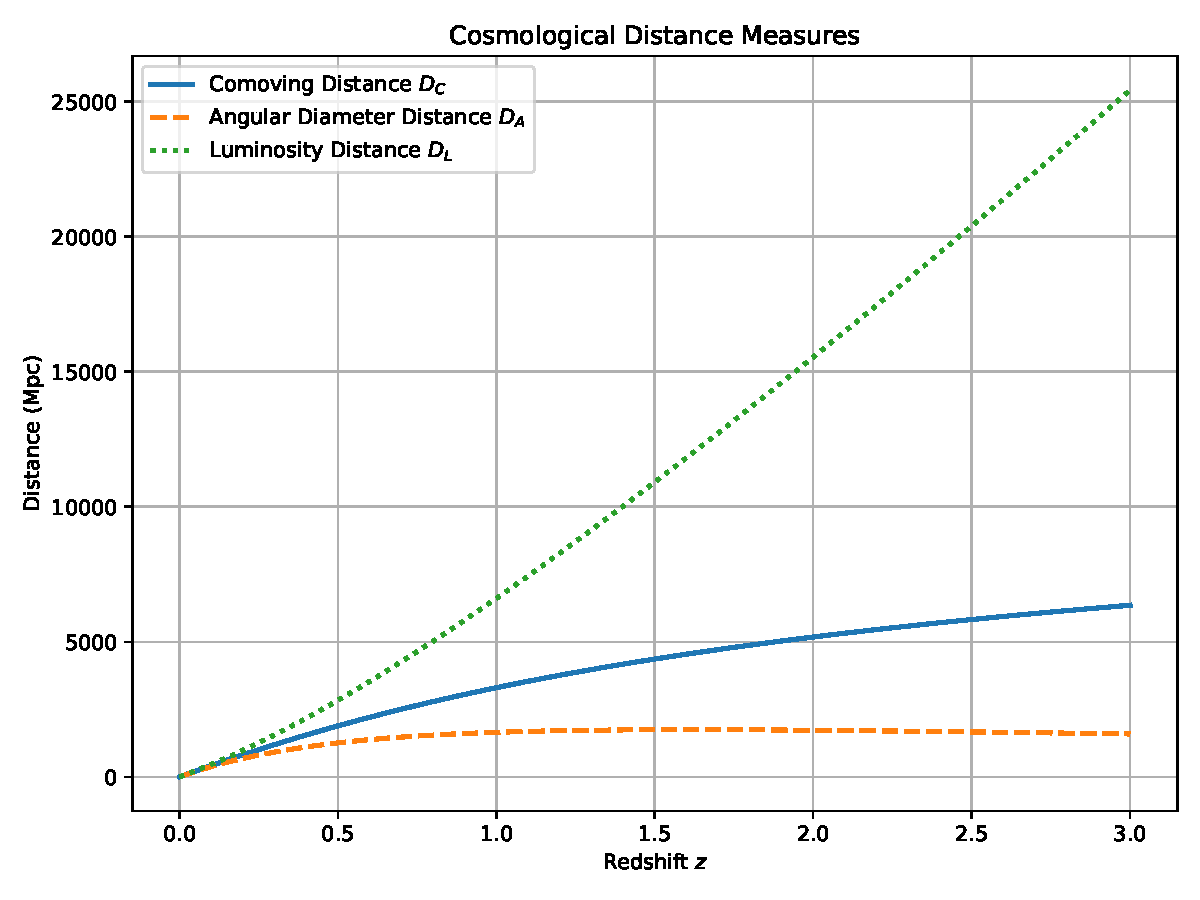
\includegraphics[width=1.0\textwidth]{MainLayout/Introduction_chapter/figures/distances.pdf}
    \caption{Different distances in cosmology plotted as a function of redshift for a flat $\Lambda$CDM with $H_0 = 70 \text{km.s}^{-1} \text{Mpc}^{-1}$ and $\Omega_m=0.3$.}
    \label{fig:hubble_riess}
\end{figure}

\section{Cosmological Observables}

In this section we will be briefly presenting some of the main observables that cosmologists are concerned with. \\

\subsection{The Cosmic Microwave Background}

During the radiation dominated era, the Universe was hot and dense, filled with a plasma of baryons and free electrons. Atoms could not form at that time because 
photons were energetic enough to ionise any neutral hydrogen immediately upon formation. As a result, baryonic matter remained tightly coupled to photons through 
Thomson scattering off free electrons. As the Universe expanded and cooled, photons eventually became insufficiently energetic to ionise hydrogen, allowing neutral atoms 
to form for the first time. This epoch is referred to as \textbf{recombination} and is associated with the decoupling of baryons and photons. The mean free path of 
photons then exceeded the Hubble radius, allowing them to travel freely across space without scattering. Today, these photons have been redshifted drastically due to the 
expansion of the Universe and are observed as a background of microwave radiation. We refer to this relic radiation as the Cosmic Microwave Background (CMB), and it 
constitutes our primary observational window onto the primordial Universe. The CMB was first discovered by Arno Penzias and Robert Wilson accidentally while calibrating 
an antenna for telecommunications and astronomy (\cite{Penzias_1965_a, Penzias_1965_b}). \\

The CMB has a nearly perfect blackbody spectrum with a mean temperature of $T_{CMB} = 2.7255 \pm 0.0006$ K (\cite{Fixsen_2009}) and temperature 
anisotropies at the level of $\Delta T / T \sim 10^{-5}$. The two-point correlation function of these anisotropies, equivalently described by the angular 
power spectrum $C_\ell$, encodes the imprint of primordial density perturbations consistent with a Gaussian random field (\cite{Planck_2018}), which later evolved 
into the large-scale structures we observe today. Secondary anisotropies, arising from effects such as gravitational lensing by galaxy clusters and inverse Compton 
scattering of CMB photons off hot intracluster gas (the Sunyaev-Zel'dovich effect), provide additional information on the late-time Universe. The polarisation of the 
CMB, decomposed into curl-free E-modes and divergence-free B-modes, further constrains inflationary models and provides a potential window onto primordial gravitational waves (\cite{Kamionkowski_1997}). \\

Through the detailed structure of the acoustic peaks in $C_\ell$, CMB observations allow precise constraints on multiple cosmological parameters, including $\Omega_m$, 
$\Omega_b$, $H_0$, $n_s$, and $A_s$ (\cite{Planck_2018_params}).\\

\begin{figure}[ht]
    \centering
    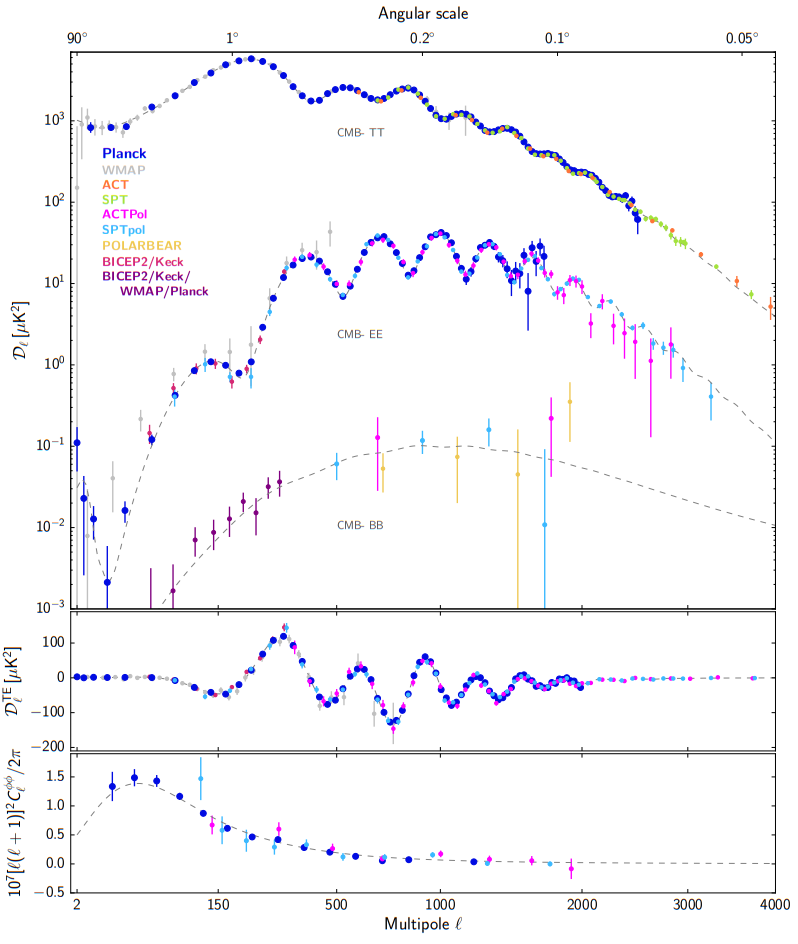
\includegraphics[width=0.7\textwidth]{MainLayout/Introduction_chapter/figures/angular_pk_cmb_.png}
    \caption{Compilation of CMB angular power spectrum measurements from \cite{Planck18_overview}.
    The upper panel shows the power spectra of the temperature and $E$-mode and $B$-mode polarization signals, the next panel the
    cross-correlation spectrum between $T$ and $E$, while the lower panel shows the lensing deflection power spectrum}
    \label{fig:pk_planck_angular}
\end{figure}

\subsection{Galaxy Surveys}

Galaxy surveys map the three-dimensional distribution of galaxies across large volumes of the Universe. Galaxies are biased tracers of the underlying matter 
distribution, and their spatial statistics allow us to infer a vast amount of information about the structure, dynamics, and history of the Universe. Surveys 
such as SDSS (\cite{York_2000}) and DESI (\cite{DESI_2016}) measure tens of millions of galaxies across a wide redshift range, from which significant cosmological 
constraints have been extracted. \\

\subsubsection{The Matter Power Spectrum}

A key statistical tool for analysing galaxy surveys is the matter power spectrum $P(k)$, defined as the variance of density fluctuations as a function of scale $k$:

\begin{equation}
    \langle \delta(\mathbf{k})\delta^*(\mathbf{k}') \rangle = 
    (2\pi)^3 \mathcal{P}(k)\,\delta^{(3)}_D(\mathbf{k} - \mathbf{k}')
\end{equation}

The shape and amplitude of $\mathcal{P}(k)$ depend directly on cosmological parameters. The primordial power spectrum can be related to late-time observations through the 
transfer function (\cite{Eisenstein_Hu_1998}):

\begin{equation}
    \mathcal{P}(k) = A_s \left(\frac{k}{k_*}\right)^{n_s - 1} T^2(k)\,D_1^2(z)
\end{equation}

where $k_* = 0.05\,\mathrm{Mpc}^{-1}$ is the pivot scale at which the primordial amplitude $A_s$ is defined (\cite{Planck_2018_inflation}), $T(k)$ is the transfer 
function encoding the scale-dependent evolution of perturbations through radiation domination, and $D_1(z)$ is the linear growth factor describing the 
growth of structure during matter domination. \\

\begin{figure}[ht]
    \centering
    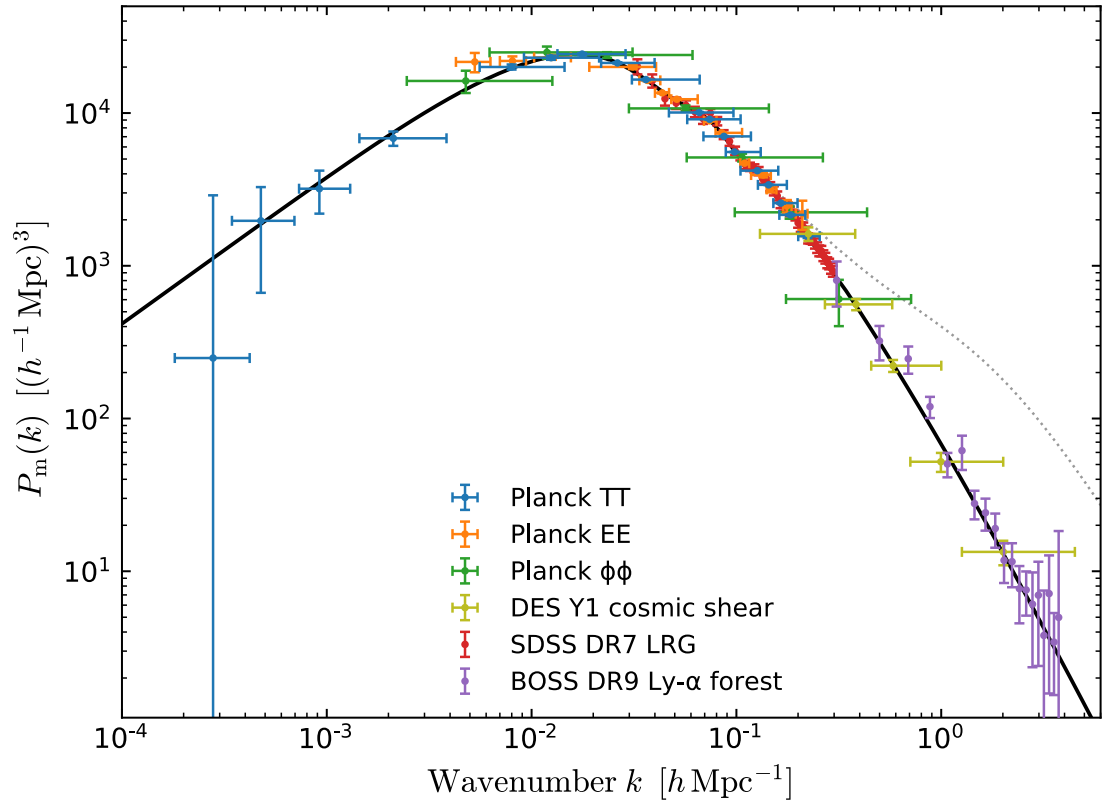
\includegraphics[width=1.0\textwidth]{MainLayout/Introduction_chapter/figures/matter_pk_planck.png}
    \caption{Linear-theory matter power spectrum (at $z=0$) inferred from different cosmological probes taken from \cite{Planck18_overview}.}
    \label{fig:pkm_planck}
\end{figure}

\subsubsection{Baryon Acoustic Oscillations}

Baryon Acoustic Oscillations (BAO) are a feature in the matter clustering that corresponds to the imprint of sound waves propagating through the baryon-photon 
plasma in the early Universe. The radiation pressure of the hot plasma drove acoustic oscillations at a sound speed of $c_s \simeq c/\sqrt{3}$. These 
oscillations were frozen in at the \textbf{drag epoch} $z_d \approx 1060$, shortly after photon decoupling at $z_* \approx 1100$, when baryons decoupled from the 
photon fluid and the sound waves could no longer propagate. The comoving distance these sound waves had travelled by that time defines the \textbf{sound horizon}:

\begin{equation}
    r_s(z_d) = \int_{z_d}^{\infty} \frac{c_s(z)}{H(z)}\,dz \approx 147\,\mathrm{Mpc}
\end{equation}

This characteristic scale is imprinted in the distribution of matter as a preferred separation between galaxies, appearing as a distinct peak in the two-point 
correlation function $\xi(r)$ at $r \approx 147$ Mpc, or equivalently as oscillations in $P(k)$. The BAO scale thus defines a \textbf{standard ruler} that 
can be measured at different redshifts to constrain the expansion history of the Universe through $H(z)$ and the angular diameter distance $D_A(z)$ 
(\cite{Eisenstein_2005}, \cite{Blake_2003}). \\

\begin{figure}
    \begin{subfigure}{.5\textwidth}
      \centering
      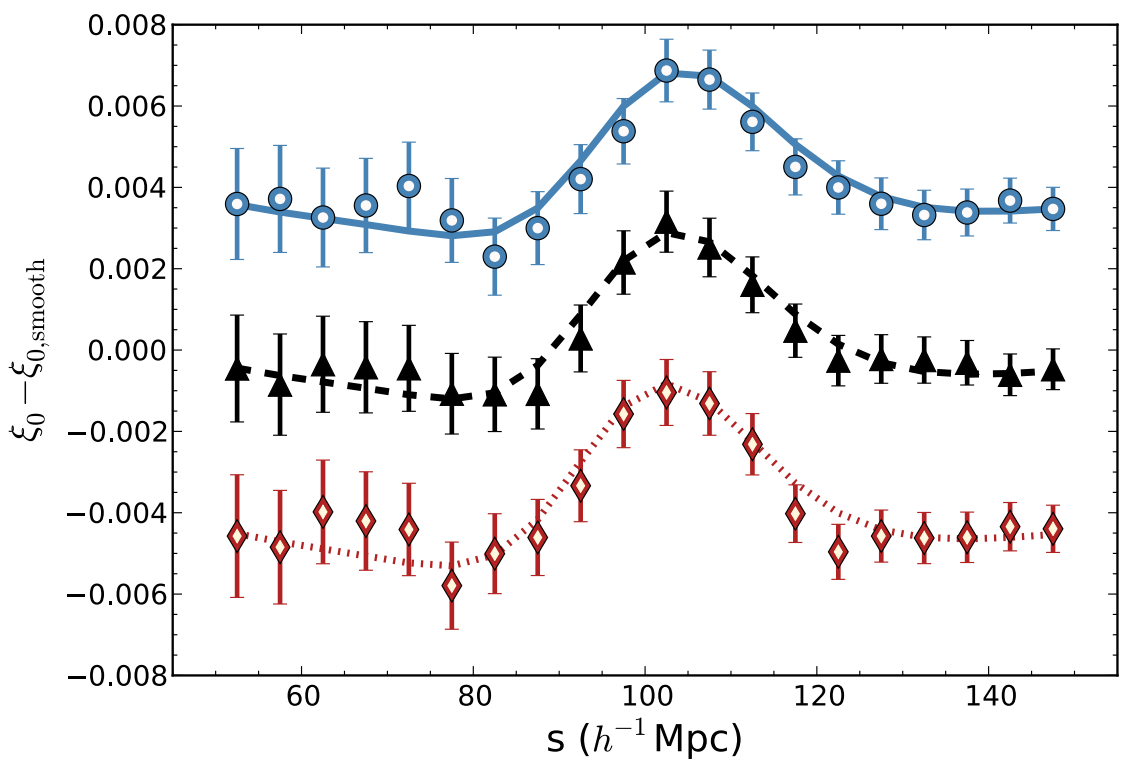
\includegraphics[width=1.\linewidth]{MainLayout/Introduction_chapter/figures/bao_corr_sdss.png}
      \caption{}
      \label{fig:bao_a}
    \end{subfigure}%
    \begin{subfigure}{.5\textwidth}
      \centering
      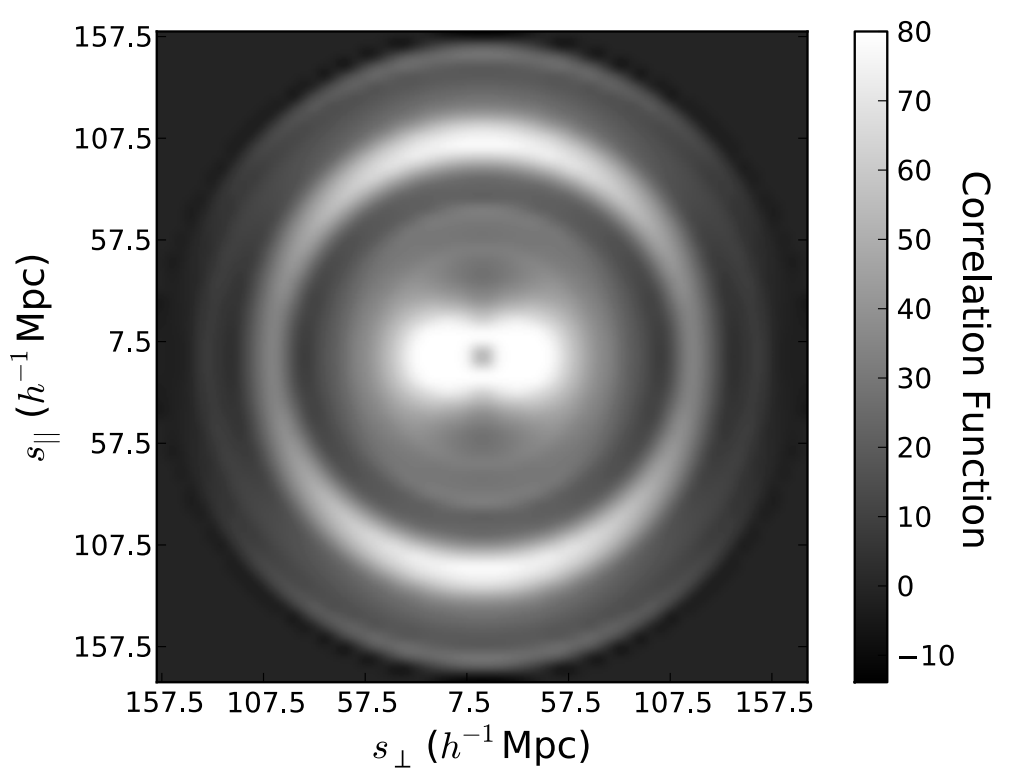
\includegraphics[width=1.\linewidth]{MainLayout/Introduction_chapter/figures/bao_corr_3d_sdss.png}
      \caption{}
      \label{fig:bao_b}
    \end{subfigure}
    \caption{BAO signals in the measured correlation functions from SDD (\cite{Alam_2017}). On the left is the smoothed prediction of the best-fitted model. On the right 
    the redshift bins are decomposed into the component of the separations transverse to and along the line of sight at $0.4<z<0.6$.}
    \label{fig:bao}
\end{figure}

\subsubsection{Redshift Space Distortions}

Galaxies are observed in redshift space rather than real space. Their peculiar velocities along the line of sight distort their apparent positions, producing 
anisotropies in the observed galaxy clustering. On large scales, coherent infall of galaxies into overdensities causes an apparent compression of structures along 
the line of sight, known as the \textbf{Kaiser effect} (\cite{Kaiser_1987}). On small scales, the virial motions of galaxies within collapsed structures produce 
an elongation of structures along the line of sight, known as the \textbf{Fingers of God} effect (\cite{Jackson_1972}). \\

The amplitude of these distortions depends on the rate of structure growth, encapsulated in the parameter $f\sigma_8$, where $f = d\ln D_1/d\ln a \approx 
\Omega_m(z)^{0.55}$ is the growth rate predicted by General Relativity and $\sigma_8$ is the amplitude of matter fluctuations on scales of $8\,h^{-1}$ Mpc. 
Modified gravity theories predict different values of $f$, making measurements of $f\sigma_8$ a direct test of GR on cosmological scales (\cite{Guzzo_2008}, 
\cite{Planck_2018_params}). \\

\subsection{Type Ia Supernovae}

As discussed in Section \ref{sec:cosmological_distances}, it is possible to obtain the distance of an object through its luminosity. However, measuring the intrinsic luminosity 
of celestial objects is a difficult task in itself. Type Ia Supernovae are thermonuclear explosions involving white dwarf stars that 
are \textbf{standardizable candles}, meaning they're characterized by a reproducible intrinsic luminosity. By measuring their apparent brightness as a function of redshift, 
one can reconstruct the luminosity distance-redshift relation $d_L(z)$ and constrain the expansion history of the Universe. 
This led to the discovery of the accelerated expansion of the Universe (\cite{Riess_1998}, \cite{Perlmutter_1999}). A detailed discussion of Type Ia 
Supernovae and their use as cosmological probes is presented in Chapter 2. \\

\subsection{Gravitational Lensing}

According to general relativity, mass curves spacetime and light follows the geodesics of that curved geometry. As a result, the path of photons is deflected 
when passing near massive objects, a phenomenon known as gravitational lensing. In a cosmological context, this deflection can be derived from the geodesic equation 
applied to the perturbed FLRW metric, and it provides a direct probe of the total matter distribution,both baryonic and dark, along the line of sight. \\

Two main regimes of gravitational lensing are relevant for cosmology. \textbf{Strong lensing} occurs in the vicinity of objects with deep gravitational potentials, such 
as massive galaxy clusters, producing dramatic and easily identifiable distortions such as multiple images, giant arcs, and Einstein rings. It provides precise 
measurements of the mass distribution of individual clusters. \textbf{Weak lensing} operates in the regime where the distortion of any individual background source is 
too small to be detected — the induced ellipticity is much smaller than the intrinsic ellipticity of a galaxy \cite{Bartelmann_2001}. However, the lensing signal can be recovered statistically 
by measuring the coherent distortion of the shapes of large samples of background galaxies, an effect known as \textbf{cosmic shear} $\gamma$. \\

Since lensing responds to all matter along the line of sight, cosmic shear surveys provide a direct measurement of the projected matter distribution. 
The amplitude of the cosmic shear signal is sensitive to both the amplitude of matter fluctuations $\sigma_8$ and the matter density $\Omega_m$, but these two parameters are largely degenerate in lensing observations. This degeneracy is 
characterised by the parameter $S_8 = \sigma_8(\Omega_m / 0.3)^{0.5}$,  which current surveys constrain to percent-level precision (\cite{KiDS_2021} \cite{DES_Y3_2022}).\\

\begin{figure}[ht]
    \centering
    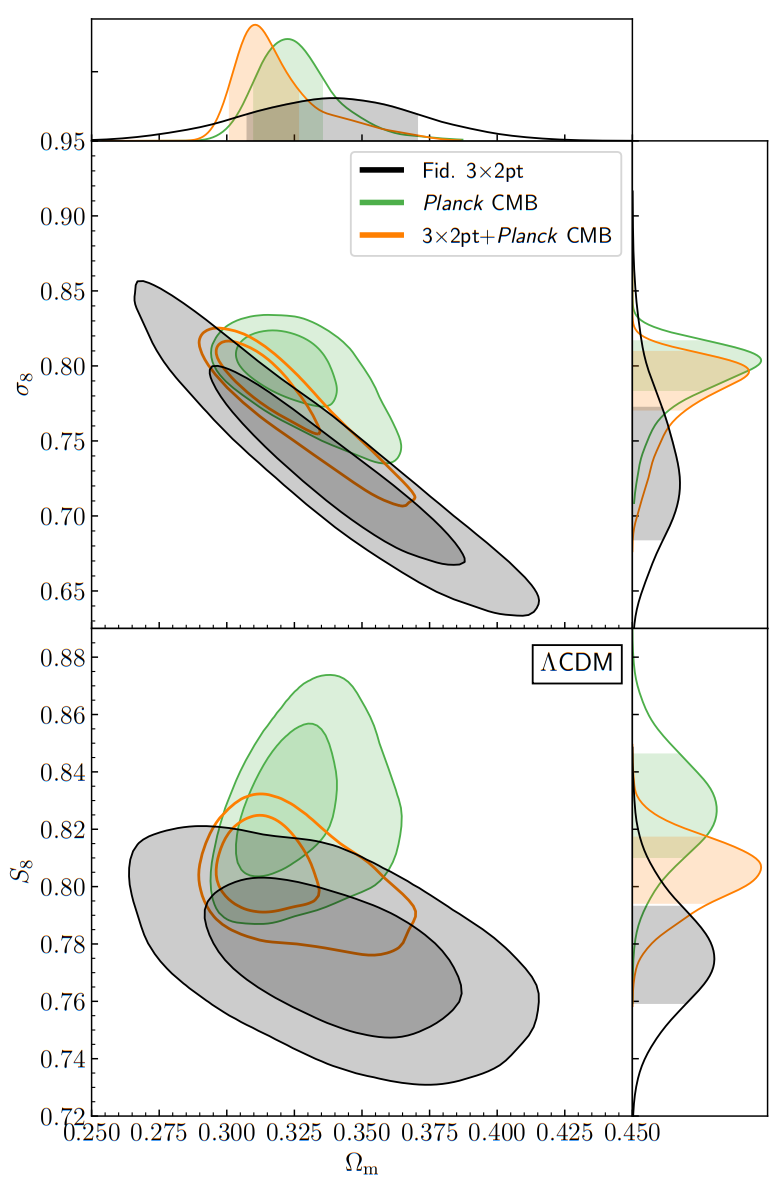
\includegraphics[width=0.6\textwidth]{MainLayout/Introduction_chapter/figures/lensing_constraints_.png}
    \caption{A comparison of the marginalized parameter constraints in the $\Lambda$CDM model from the Dark Energy Survey (\cite{DES_Y3_2022}) with predictions from Planck CMB data (no lensing; green). There is also the fiducial cosmology 3x2pt (black) and the combined Y3 3x2pt and Planck (orange) results.}
    \label{fig:lensing}
\end{figure}


\subsection{The Lyman-$\alpha$ Forest}

When observing the spectra of distant quasars, a dense series of absorption lines is observed, a feature known 
as the \textbf{Lyman-$\alpha$ forest}. These absorption lines are produced by neutral hydrogen clouds in the intergalactic medium (IGM) through which the quasar 
photons pass on their way to the observer, typically at redshifts $2 \lesssim z \lesssim 5$. Each absorbing cloud at redshift $z$ produces an absorption line at 
an observed wavelength:
\begin{equation}
    \lambda_{obs} = 1216\,(1+z)\;\text{\AA}
\end{equation}
where $1216\,\text{\AA}$ is the restframe Lyman-$\alpha$ wavelength. It's possible to show that the neutral hydrogen fraction in the IGM traces the 
underlying total matter density field, making the Lyman-$\alpha$ forest an effective map of the matter distribution along the line of sight 
(\cite{Gunn_1965}). \\

The cosmological information in the Lyman-$\alpha$ forest is extracted through the power spectrum of the transmitted flux fluctuations, which can be directly related 
to the three-dimensional matter power spectrum (\cite{Croft_1998}). A particularly powerful feature of this probe is that it is sensitive to scales 
$k \sim 0.1$--$10\,h\,\mathrm{Mpc}^{-1}$ at high redshift, well beyond the reach of galaxy surveys, making it highly complementary to both CMB and galaxy clustering 
measurements. This sensitivity to small scales and high redshifts allows the Lyman-$\alpha$ forest to constrain the sum of neutrino masses $\sum m_\nu$ through 
the small-scale suppression of the power spectrum (\cite{Palanque_2015}), the spectral index $n_s$ and the BAO standard ruler at $z \sim 2.3$ 
(\cite{Delubac_2015}).\\

\begin{figure}[ht]
    \centering
    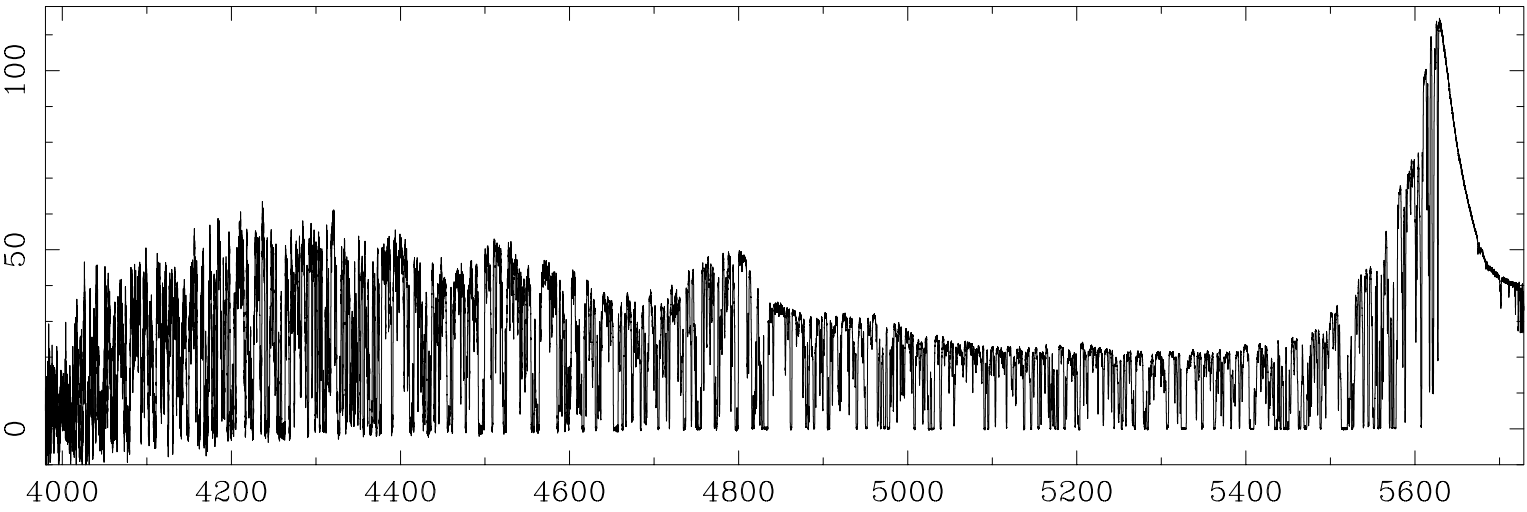
\includegraphics[width=1.0\textwidth]{MainLayout/Introduction_chapter/figures/lya.png}
    \caption{High resolution spectrum of the Lyman-$\alpha$ forest part of a quasar measured at $z=3.63$ taken with the HIRES spectrograph on the 10 m Keck telescope in Hawaï.}
    \label{fig:lyman_alpha}
\end{figure}

\section{Tensions in the Cosmological Model} \label{sec:tensions}

The previous sections served to introduce and demonstrate the power of the $\Lambda$CDM model in describing the Universe. Nonetheless, tensions have emerged 
between cosmological parameter measurements obtained from different probes, suggesting that the discrepancies may be of physical or systematic origin. 
Here we present the three main tensions. \\

\subsection{$H_0$ Tension}

The Hubble constant $H_0$ can be inferred in two ways: through direct measurements via the cosmic distance ladder, or indirectly through model-dependent fitting of 
early-Universe observables. The direct measurement is obtained by calibrating standard candles such as Cepheid variables and Type Ia supernovae. 
Results from the SH0ES collaboration give $H_0 = 73.04 \pm 1.04\,\text{km}\,s^{-1}\,\text{Mpc}^{-1}$ (\cite{Riess_2022}). The indirect method relies on fitting the acoustic peak 
structure of the CMB angular power spectrum within the $\Lambda$CDM framework. The Planck 2018 collaboration reports $H_0 = 67.4 \pm 0.5\,\text{km}\,s^{-1}\,\text{Mpc}^{-1}$ 
(\cite{Planck_2018_params}), yielding a $\sim 5\sigma$ discrepancy with the SH0ES result. We see this in Figure \ref{fig:h0_tension}. This tension persists across multiple independent measurements of $H_0$ 
(\cite{DiValentino_2021}), raising the question of whether it reflects unknown systematic errors, or new physics beyond $\Lambda$CDM present at different 
epochs of the Universe. Recent results from the Chicago-Carnegie Hubble Program (CCHP) (\cite{Freedman_2025}) have measured the $H_0$ value using independent data from the James Webb Space Telescope 
with three independent methods (Tip of the Red Giant Branch (TRGB), J-Region Asymptotic Giant Branch (JAGB) and Cepheids). Their results show that with TRGB and 
JAGB the $H_0$ values are compatible with Planck measurements indicating that the tension arises from systematic effects. Moreover, a recent study by \cite{Stiskalek_2025} explicitly accounted 
for peculiar velocities when measuring $H_0$ using the same data as the one used in SH0ES and obtained a smaller value than the one reported by SH0ES of $H_0 = 71.1\pm 1.4 \, \text{km}\,s^{-1}\,\text{Mpc}^{-1}$ highlighting the importance of modeling peculiar velocities. 
The paper also highlights that whether the sample selection is done on supernova magnitude or host galaxy redshift does not significantly impact the value of $H_0$. 
Figure \ref{fig:h0_tension} shows $H_0$ measurements from different probes, highlighting the tension. \\

\begin{figure}[ht]
    \centering
    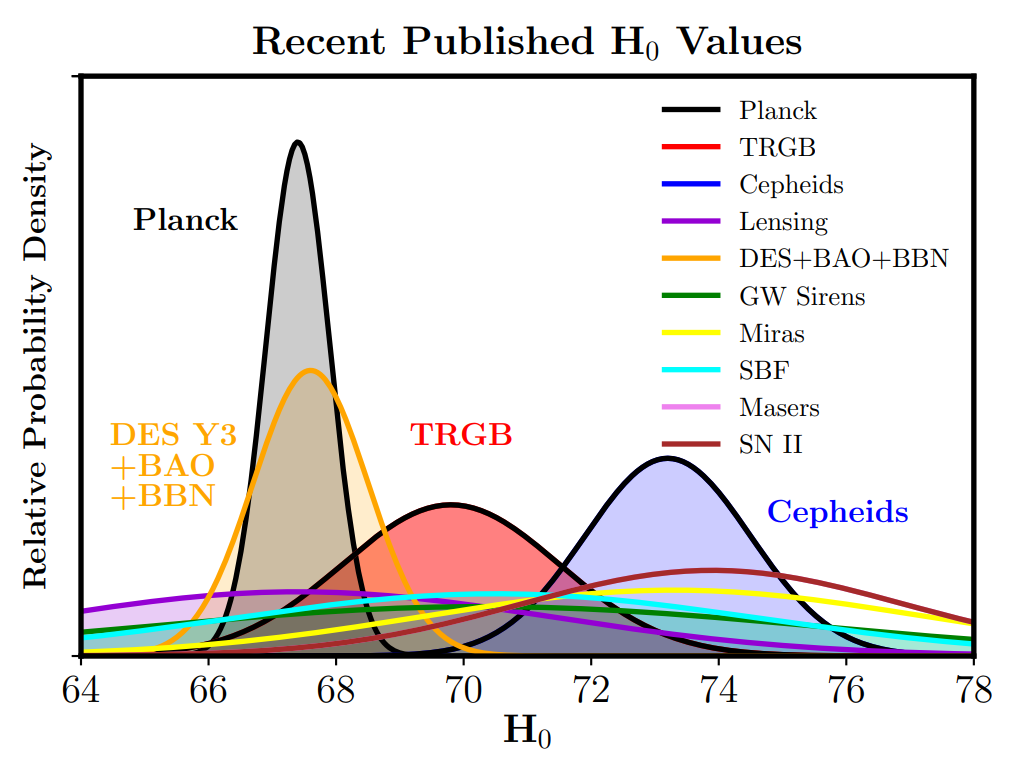
\includegraphics[width=0.8\textwidth]{MainLayout/Introduction_chapter/figures/h0_tension.png}
    \caption{Probability density functions of $H_0$ from different measurements probed at different redshifts, taken from \cite{Freedman_2021}. The CMB measurements prefer a lower $H_0$ value while Cepheids prefer higher values.}
    \label{fig:h0_tension}
\end{figure}

\subsection{$S_8$ Tension}

The parameter $S_8 = \sigma_8\sqrt{\Omega_m/0.3}$ combines the amplitude of matter fluctuations $\sigma_8$ with the matter density $\Omega_m$, and 
characterises the growth of large-scale structure. It can be measured both through the spatial correlations of galaxies and weak gravitational lensing, and through 
the CMB anisotropy power spectrum, where it is related to the primordial amplitude $A_s$ through the linear growth of structure. The Planck 2018 collaboration 
measures $S_8 = 0.832 \pm 0.013$ (\cite{Planck_2018_params}), while the Dark Energy Survey Year 6 measures $S_8 = 0.789^{+0.012}_{-0.012}$ from a combination 
of cosmic shear, galaxy clustering, and galaxy-galaxy lensing (\cite{DES_y6}), indicating a $2.3\sigma$ discrepancy (Figure \ref{fig:s8_tension}). \\

\begin{figure}[ht]
    \centering
    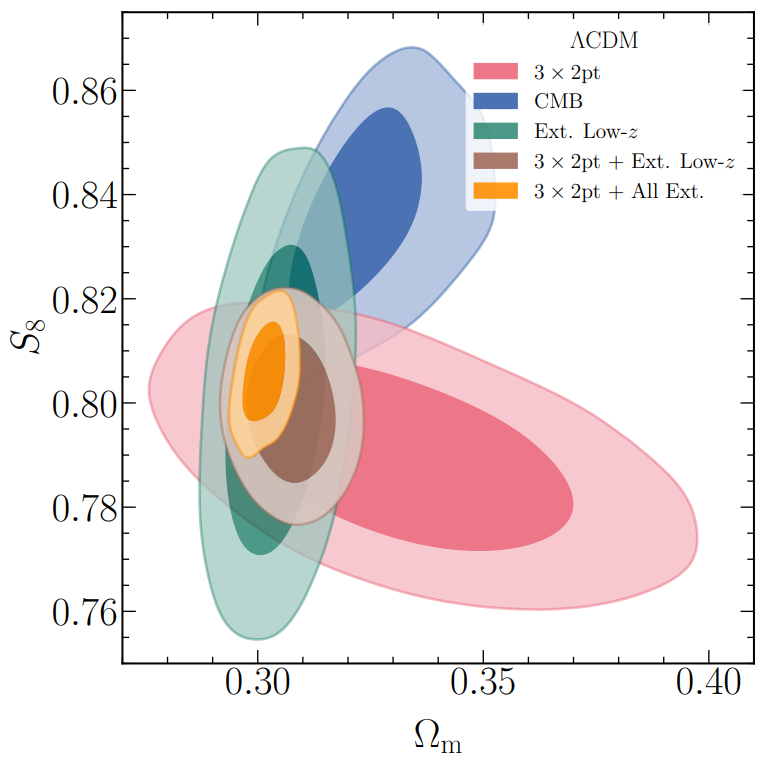
\includegraphics[width=0.8\textwidth]{MainLayout/Introduction_chapter/figures/s8_tension_des.png}
    \caption{$S_8$ and $\Omega_m$ contours for different galaxy surveys and CMB taken from \cite{DES_y6} enclosing the 68\% and 95\% posterior probability. The combination of the DES results with all of the other probes is in orange while the CMB measurements are in blue.}
    \label{fig:s8_tension}
\end{figure}

\subsection{$(w_0, w_a)$ Tension}

Within the $\Lambda$CDM paradigm, the accelerated expansion of the Universe is driven by a cosmological constant with equation of state $w = -1$, corresponding 
to a constant dark energy density $\rho_\Lambda = \text{const}$. If instead the dark energy density evolves with time, the simplest extension is the 
Chevallier-Polarski-Linder (CPL) parametrisation (\cite{Chevallier_2001}, \cite{Linder_2003}): 
\begin{equation}
    w(a) = w_0 + w_a(1-a)
\end{equation}
where $w_0$ is the present-day equation of state and $w_a$ parametrises its time evolution. The $\Lambda$CDM limit is recovered for $w_0 = -1$ and $w_a = 0$. \\

Recent results from DESI DR2, when combined with Planck CMB data and Type Ia supernova datasets, show deviations from $\Lambda$CDM in the $(w_0, w_a)$ plane 
(\cite{DESI_DR2_2025}). The significance of the deviation depends on the supernova sample used: $2.8\sigma$ when combined with Pantheon+, $3.8\sigma$ with 
Union3, and $4.2\sigma$ with DES Year 5 (Figure \ref{fig:w0_tension}) (\cite{DESI_DR2_2025}). A subsequent recalibration of the DES Year 5 supernova sample (DES-SN5YR, \cite{Popovic_2025}) reduced 
this DES discrepancy to $3.2\sigma$. \\

\begin{figure}[ht]
    \centering
    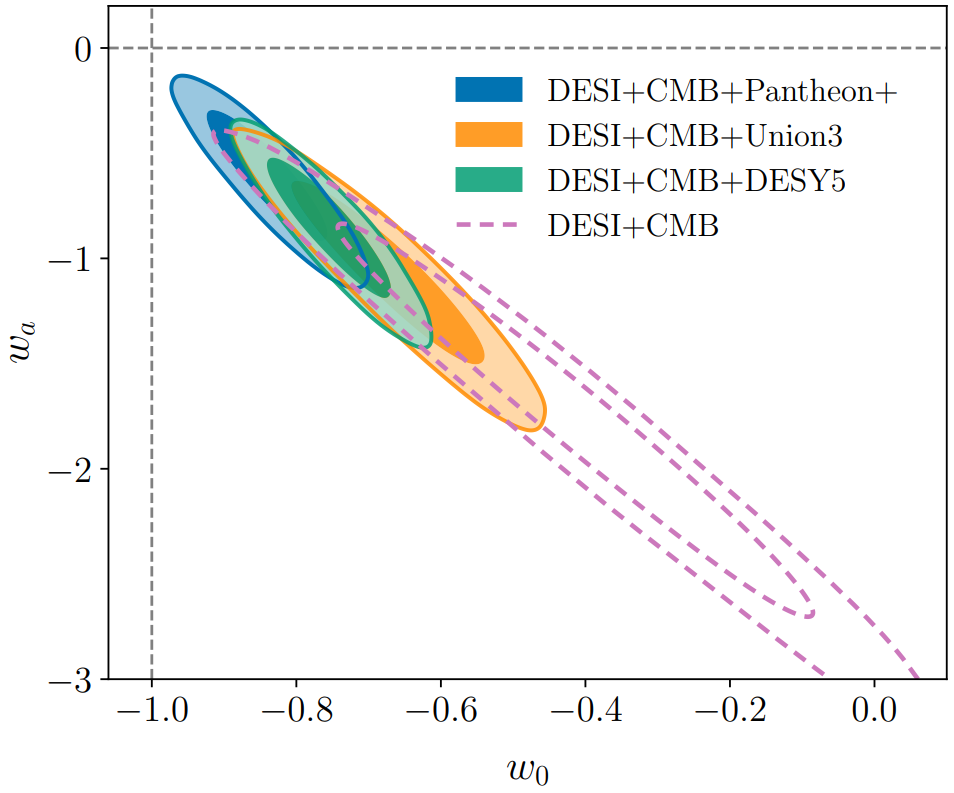
\includegraphics[width=0.8\textwidth]{MainLayout/Introduction_chapter/figures/w0_wa_tension.png}
    \caption{$w_0$ and $w_a$ contours from the latest \cite{DESI_DR2_2025} measurements enclosing the 68\% and 95\% posterior probability when 
    combined with Pantheon+ (blue), Union3 (orange) and DES-SN5YR (green) and CMB (purple dotted lines). }
    \label{fig:w0_tension}
\end{figure}
\section{Physical Explanations for the Accelerated Universe}

Since the discovery of the accelerated expansion of the Universe by 
\cite{Riess_1998} and \cite{Perlmutter_1999}, understanding its underlying origin has 
become one of the major challenges in modern cosmology. One possible explanation is the 
introduction of a cosmological constant $\Lambda$ in Einstein's equations. This constant 
can be interpreted in different ways: as a geometrical contribution modifying the Einstein 
equations, as an effective fluid with a constant energy density and equation of state 
$w=-1$, or as a manifestation of the vacuum energy of quantum fields. When interpreted 
as an additional energy component driving the accelerated expansion, it is referred to as 
dark energy. In the following subsections, we discuss several theoretical models proposed 
to explain the observed accelerated expansion.

\subsection{Cosmological Constant} \label{sec:expanding_universe}

The simplest way to account for the acceleration as we have mentioned before is by adding a cosmological constant $\Lambda$ to the Einstein equations \ref{eqn:einstein_lambda}, 
which is what is done in the $\Lambda$CDM model. We can look at $\Lambda$ in two equivalent ways, either a modification to the geometry of spacetime or as a part of the 
energy content of the Universe. Mathematically they are equivalent since the energy-momentum tensor $T_{\mu \nu}$ can include the $\Lambda g_{\mu \nu}$ and their 
equations of state are indistinguishable in $\Lambda$CDM. \\

\subsection{Dynamical Dark Energy}

One could naturally assume that if the acceleration of the Universe is driven by a fluid, its energy density would change throughout time. The common way to model this 
is with the Chevallier-Polarski-Linder (CPL) model (\cite{Chevallier_2001}) characterized by two parameters $w_0$ and $w_a$ such that:
\begin{equation}
    w(z) = w_0 + w_a \frac{z}{1+z} = w_0 + w_a(1-a)
\end{equation}
Therefore the Hubble parameter becomes:
\begin{equation}
    H(z) = H_0 \sqrt{\Omega_m(1+z)^3 + \Omega_r(1+z)^4 + \Omega_k(1+z)^2 + e^{\left( -3w_a\frac{z}{1+z} \right)} \Omega_{\text{DE}}(1+z)^{3(1+w_0+w_a)} }
\end{equation}
where $\Omega_{\text{DE}}$ is the energy density of this dynamical dark energy. $\Lambda$CDM then becomes a particular case where $w_0=-1$ and $w_a=0$.

\subsection{Quintessence Field}

The quintessence model uses an approach similar to inflation where one assumes the accelerated expansion is driven by a scalar field $\phi$, here called the quintessence field. 
The action associated to that field is written as:
\begin{equation}
    S(\phi) = \int d^4x \sqrt{-g}\left( -\frac{1}{2} g^{\mu \nu} \partial_{\mu}\phi \partial_{\nu} \phi - V(\phi) \right)
\end{equation}
The equations of motion of $\phi$ are determined by the Klein-Gordon equation:
\begin{equation}
    \ddot{\phi} + 3H \dot{\phi} + \frac{d}{d\phi}V = 0
\end{equation}
For a FLRW metric, the pressure and energy density become:
\begin{equation}
    P_{\phi} = \frac{1}{2}\dot{\phi}^2 - V(\phi)
\end{equation}
\begin{equation}
    \rho_{\phi} = \frac{1}{2}\dot{\phi}^2 + V(\phi)
\end{equation}
This gives the following equation of state:
\begin{equation}
    w = \frac{P_{\phi}}{\rho_{\phi}} = \frac{\frac{1}{2}\dot{\phi}^2 - V(\phi)}{\frac{1}{2}\dot{\phi}^2 + V(\phi)}
\end{equation}
Under a slow-roll approximation, the field evolves slowly such that $\dot{\phi} \simeq 0$ giving us $w\approx -1$ where we recover the results 
of a cosmological constant. If we consider a fast rolling field where the potential is negligible in front of the evolution, the equation of state becomes $w\approx 1$ 
however this is not possible since we know that for an accelerating Universe $w<-\frac{1}{3}$. Results from \cite{DESI_DR2_2025} show a preference for a 
dynamical dark energy in the CPL parameterization. \\ 

\subsection{Modified Theories of Gravity} \label{sec:modified_gravity}
An alternative to dark energy is to modify the theory of GR on cosmological scales. We call the models that do so Modified Gravity models (MG). Multiple classes of MG theories 
exist each modifying a certain aspect of GR. We will be presenting some of those models in each class.\\

\noindent \textbf{\underline{Additional scalar fields}} \\

The first class consists of adding an additional scalar field to the Einstein-Hilbert action. These fields need to have equations of motions of second-order time derivatives 
at most to avoid any unphysical solutions. \\

Models in this class include the $f(R)$ models (\cite{Sotiriou_2010}) which replaces the Ricci scalar $R$ by a general function of $R$. The action for an $f(R)$ gravity becomes:
\begin{equation}
    S = \frac{c^4}{16\pi G}\int \sqrt{-g} f(R) d^4x + \int \sqrt{-g} \mathcal{L}_m d^4x
\end{equation}
And the field equations are:
\begin{equation}
    f'(R)R_{\mu \nu} - \frac{1}{2}f(R)g_{\mu \nu} + [g_{\mu \nu}\Box -\nabla_{\mu}\nabla_{\nu}]f'(R) = \frac{8 \pi G}{c^4}T_{\mu \nu}
\end{equation}
For the simplest case $f(R)=R-2\Lambda$ we recover GR. For a FLRW metric, the Friedmann equations become (with $c=1$):
\begin{equation}
    3f'H^2 = 8\pi G \rho_m + \frac{1}{2}(f'R-f) - 3H \dot{f'}
\label{eqn:friedmann_fR}
\end{equation}
\begin{equation}
    -2f'\dot{H} = 8 \pi G (\rho_m + P_m) + \ddot{f'} - H \dot{f'}
\end{equation}
If one rewrites Equation \ref{eqn:friedmann_fR} to match what we get in GR $3H^2 = 8\pi G\rho$, we can identify an effective "curvature fluid" that under certain conditions 
would cause an accelerated Universe. This gives us an effective equation of state on $w_{eff}$:
\begin{equation}
    w_{eff} = -1 + \frac{1}{3f'H^2}\left[8\pi G(\rho_m + P_m) + \ddot{f'} - H \dot{f'} \right]
\end{equation}
Since acceleration is possible for $w<-\frac{1}{3}$ this means that a condition on any $f(R)$ theory would be:
\begin{equation}
    8\pi G(\rho_m + P_m) + \ddot{f'}-H\dot{f'}<2f'H^2
\end{equation}
$f(R)$ must also be able to reproduce GR during the early Universe and at high matter density regions to remain consistent with observational results. This screening effect is called 
the chameleon mechanism and the best-known $f(R)$ theories do possess it. \\

\noindent \textbf{\underline{Massive gravity}} \\
In quantum field theory, forces are mediated by particles, for instance photons for electromagnetism and gluons for the strong force. 
By analogy, gravity is expected to be mediated by a spin-2 particle called the graviton. The graviton is predicted to be a massless 
particle with an infinite interaction range, that can recover GR in a quantum field theory formalism. If we now assume that the graviton does in fact possess a mass, that would 
decrease the range of its gravitational interaction as well as its strength between distant objects (\cite{Fierz_1939}, \cite{deRham_2011}). The gravitational potential is then modified as follows:
\begin{equation}
    \Phi = - \frac{GM}{r}e^{-mr}
\end{equation}
where $r$ is the distance to an object, $M$ the mass of the object and $m$ the mass of the graviton. However, the introduction of massive gravitons produces multiple 
instabilities such as the inability to recover GR when $m$ goes to 0. It also has difficulty producing flat FLRW solutions.\\

\noindent \textbf{\underline{Breaking assumptions}} \\

The last class of models we will present here are the ones that break physical assumptions. Here we present an example of a model proposed by Gia Dvali, Gregory Gabadadze 
and Massimo Porrati (\cite{Dvali_2000}) where gravity can propagate in a 5-dimensional spacetime with an additional spatial dimension. We can think of it as our 4D world embedded 
in an infinite volume 5D space. The idea being that the gravity on large scales appears to be in 5D while on small scales in 4D, this is due to the Vainshtein effect. 
The action for such a theory looks like :
\begin{equation}
    S = 2M_5^3 \int d^5X \sqrt{-\tilde{g}}\tilde{R} + 2M_{pl}^2 \int d^4x \sqrt{-g}R + \int \sqrt{-g}\mathcal{L}_m + S_{GH-} + S_{GH+}
\end{equation}
where $M_5$ is the Planck mass $M_{pl}$ in 5D, $\tilde{g}$ and $\tilde{R}$ are the norm of the metric and the Ricci scalar in 5D. The $S_{GH-}$ and $S_{GH+}$ are Gibbons-Hawkings-York 
terms that serve as boundary terms commonly found in, but not limited to, quantum gravity theories.\\ 
The theory does predict a late time acceleration (\cite{Deffayet_2001}), however it suffers theoretical instabilities and unphysical solutions (\cite{Koyama_2007}). 
Observations have also ruled the theory out 
DGP theories (\cite{Fang_2008}). \\



\chapter{Cosmology with Type Ia Supernovae}\label{chap2}
\minitoc 
\section{Type Ia Supernova} \label{sec:sn_ia}

For many centuries, astronomers all over the globe would observe the emergence of a bright light in the sky thinking it was the birth of a new star in the Universe. 
In 1572, an astronomer by the name of Tycho Brahe developped an interest in such event and named the phenomenon \textit{nova stella}, latin for new star. 
His work inspired later astronomers suhc as Kepler and eventually lead to the Copernicean revolution.\\

It wasn't until 1934 when Fritz Zwicky and Walter Baade when the term supernova (from the latin "super" and "novae" meaning new bright stars) was coined to describe the 
brightest novae observed. The supernova classifies phenomena related to the end of a star's life cycle when they go through explosions. This process is temproary therefore 
taking part in the class of \textbf{transients}. Their fluxes are initially weak and then increases over time to a point where it becomes detectable from 
the Earth, then it diminishes slowly till it disapears.\\

In the next sections we will be explaining the different classifications of supernovae as well as our understanding behind their explosion mechanisms. A particular focus 
will be on a specific class of supernovae called "type Ia" and why they are heavily studied by cosmologists. \\

\subsection{Classification}

Two main categories of supernovae exists: type I and tpye II each with their own subcategories of supernovae. These main categories were discovered by Rudolph Minkowskia and 
Walter Baade in 1941 when studying the spectral features of 14 supernovae. Type I supernovae's absorption spectra is characterized by having no Hydrogen, contrary to type II. 
Type I supernova are then divided in two three classes (\cite{Wheeler_1985, Elias_1985}, \cite{Wheeler_1990}):
\begin{itemize}
    \item \textbf{Ia}: contains Silicon line at $615.0$ nm
    \item \textbf{Ib}: does not contain Silicon and contains Helium line at $587.6$ nm 
    \item \textbf{Ic}: does not contain Silicon or Helium lines
\end{itemize}

\noindent Type II supernova are divided in following way (\cite{Hillier_2019}):
\begin{itemize}
    \item \textbf{IIn}: contains narrow absoption lines
    \item \textbf{IIb}: contains Helium like Ib 
    \item \textbf{IIP}: Hydrogen dominates the spectra and its integrated flux becomes constant
    \item \textbf{IIL}: Hydrogen dominates the spectra and its integrated flux decreases in time
\end{itemize}

\noindent The classification of supernovae can be summarized in Figure \ref{fig:sn_classification}.

\begin{figure}[ht]
    \centering
    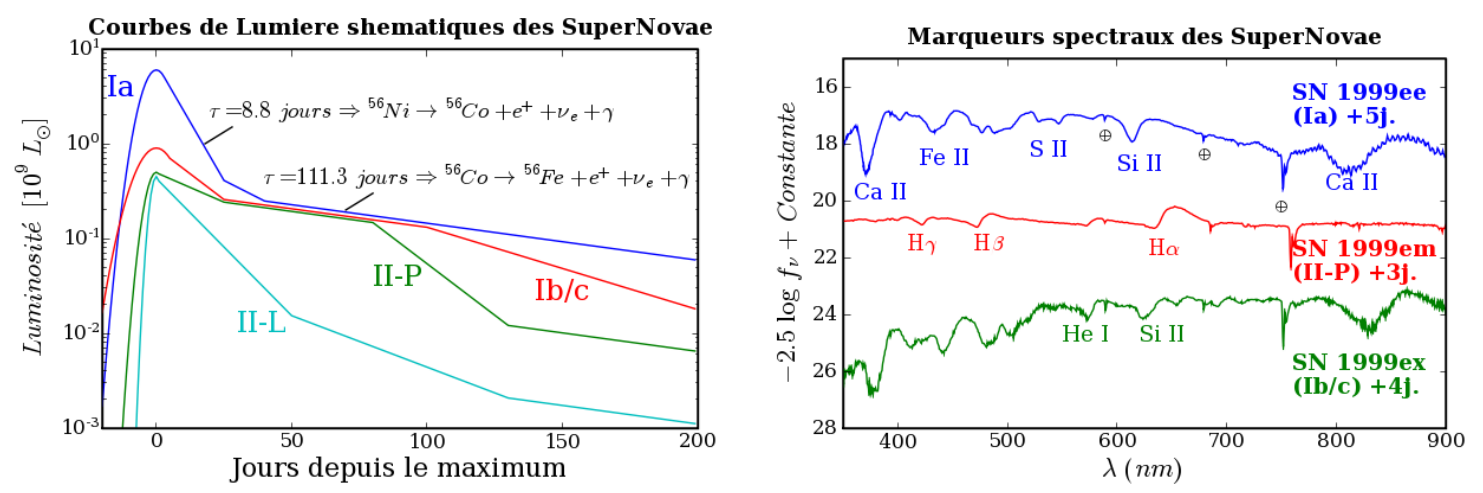
\includegraphics[width=1.0\textwidth]{MainLayout/Second_chapter/figures/sn_class_lc_spec.png}
    \caption{Photometric and spectroscopic curves for different classes taken from \cite{Baumont_2007}. 
            The left are the schematics for the integrated fluxes (lightcurves) for SN Ia (blue), SN Ib or Ic (red), SN IIP (green) and SN IIL(cyan). 
            On the right we have the spectra of three supernovae observed in 1999, SN Ia (blue), SN IIP (red) and SN Ic (green).}
    \label{fig:sn_classification_spec}
\end{figure}

\begin{figure}[ht]
    \centering
    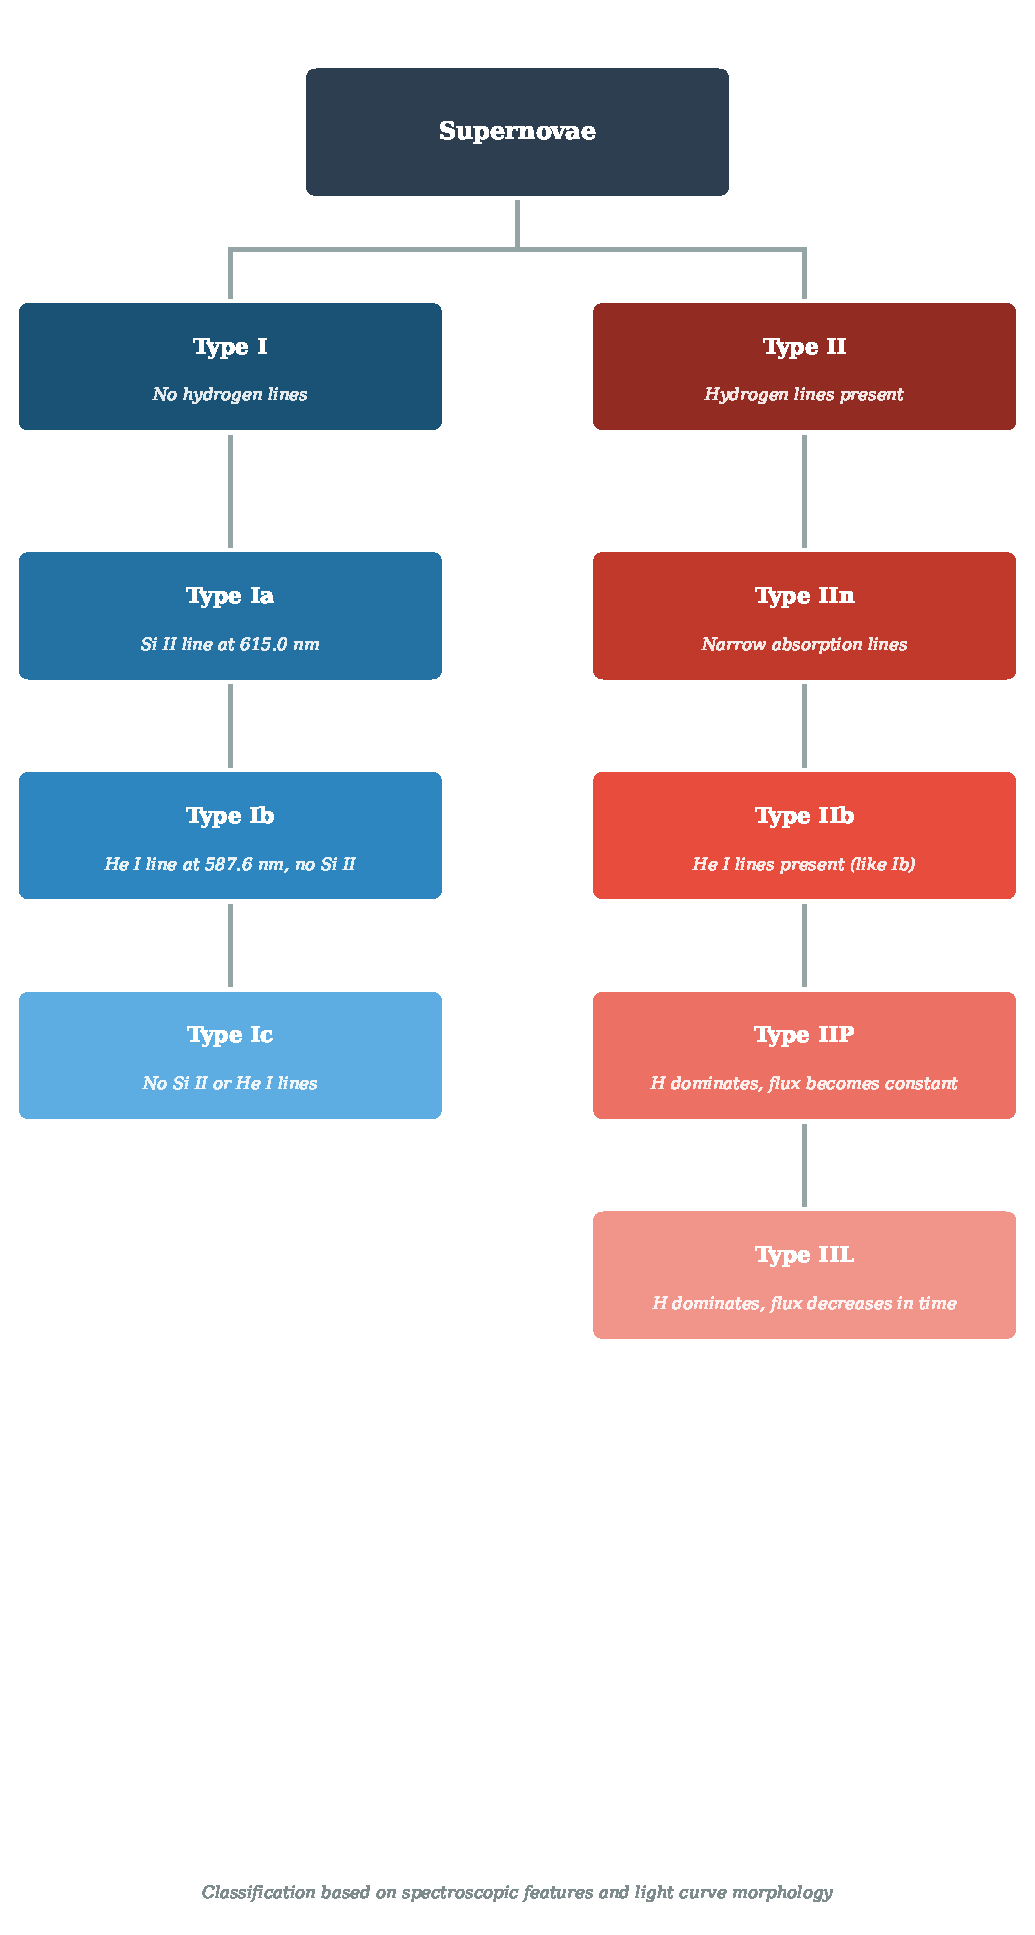
\includegraphics[width=0.7\textwidth, trim=0cm 9cm 0cm 0cm, clip]{MainLayout/Second_chapter/figures/sn_classification_vertical.pdf}
    \caption{Classification of supernovae. The left column are type I (blue) and the right column are tpye II (red).}
    \label{fig:sn_classification}
\end{figure}

\subsection{Explosion mechanisms}

Different explosion mechanisms and progenitors exist for the different classes of supernovae. We will be separating them into two cases: core-collapse and thermonuclear.\\

\noindent \textbf{\underline{Core collapse}} \\

This explosion concerns supernovae of types Ib, Ic and all types II. The occurence of this explosion happens at the end of the life cycle of a star after it has 
completed the fusion of its light elements. The star then does generate enough energy to compensate for the gravitational pull and then collapes on itself. The material 
of the star collapses until it reaches scales at which it is stopped by the strong nuclear interaction, which defines the limiting distance between atoms. This causes a collision 
between the different layers of the star creating a shock wave  that propulses the star material and ignites the supernova explosion. If the star has a mass inferior to 
$\sim 3.3M_{\odot }$ (Oppenheimer-Volkoff limit \cite{Oppenheimer_1939}), where $\bigodot$ denotes the Solar mass, the star will become neutron star. Larger mass stars turn to black holes.\\



\noindent \textbf{\underline{Thermonuclear}} \\

Thermonuclear explosions concern tpye Ia supernovae. This occurs in white dwarf stars comprised primarily of Oxygen and Carbon when their masses approach the Chandrasekhar limit 
of $\sim 1.44M_{\odot }$ (\cite{Chandrasekhar_1931}). White dwarf stars form from the remains of low mass stars (typically under $8M_{\odot}$) and are dense degenerated systems. 
This term comes from the fact that the density of a white dwarf is limited by electron degeneracy pressure that comes from the Pauli exclusion principle which states that 
two electron within the same energy levels cannot share the same quantum state. Accreting more mass from external sources induces Carbon and Oxygen fusion which increases 
the temperature of the white dwarf stars. If the accretion keeps on happening, the fusion of Carbon and Oxygen becomes a chain reaction at a constant pressure causing a 
thermonuclear explosion (\cite{Ropke_2004}). The explosion ends up releasing around $10^{51}$J of energy, mainly kinetic energy. Only a fraction of that is turned into luminous energy 
of $10^{44}$J (\cite{Khokhlov_1993}) meaning tpye Ia supernovae have a luminosity at the same order of magnitude of its host galaxy. \\

Observations such as SN2011fe have demonstrated that type Ia supernovae are originated from compact and dense stars, which are white dwarfs. It also important to note that 
tpye Ia supernova spectra are characterized by Silicium and Calcium absoption lines which are the product of the Carbon and Oxygen fusion. Due to the fact that 
type Ia supernovae occur in quasi-identical environments, we tend to observe similar luminosities between them. Finally, they are observed in environments with older stars 
which is justified due to the fact that white dwarfs happen at the final stages of a star. \\

White dwarf stars aren't very luminous to be observed at long distances. Usually they are detected a short while after their explosions. Therefore the progenitors of type Ia 
supernovae have never been observed. Multiple scenarios exist to explain the explosions. We will only be presenting the two main scenarios:
\begin{itemize}
    \item \textbf{Single degenerate} (\cite{Nomoto_1982}): This occurs when white dwarfs accrete mass from nearby more massive non-degenerate stars will low surface gravity, like red giants. 
Arguments against that scenario is that the accreted Helium and Hydrogen must all be transformed into Carbon and Oxygen with a fusion reaction, which would explain why they do not appear as absorption line 
in the spectrum of the supernova. The other is that the speed of the accretion can neither be too slow nor too fast or the explosion doesn't happen. Lastly, the companion stars 
weren't observed near the explosion area (\cite{Li_2011}).
    \item \textbf{Double degenerate} (\cite{Iben_1984}): This occurs when a white dwarf star accretes its mass from a nearby less massive white dwarf star in close orbit. This scenario does explain
the absence of Helium and Hydrogen absoption lines and the observation of superluminous supernovae (like \cite{Howell_2006}). It also allows for the case of a double detonation which when it happens 
for two white dwarfs who's masses are inferor to the Chandrasekhar mass can explain the existence of subluminous supernovae (\cite{Tanikawa_2019}).
\end{itemize}


\subsection{Explosion rate}

The explosion rate of type Ia supernovae is the measurement of the number of explosion at a certain redshift in year. 
It can be divided into two categories: low redshift up to $z \sim 0.3$ and hight redshift. At low redshift the explosion is nearly constant 
and barely evolves. Low redshift samples such as ZTF allow us to measure that rate. A study done by \cite{Perley_2020} on the ZTF sample, assuming an isotropic distribution, 
have measured a rate of
\begin{equation}
    R_{ZTF} = (2.35 \pm 0.24) \times 10^{4} \text{Gpc}^{-3}.\text{yr}^{-1}
\end{equation}
Where each supernova was weighted by the volume it probes with a varying limiting absolute magnitude. 
However, a recent paper by \cite{Lordet_2026} showed that the rate of supernova is explosion might be more complex than anticipated and is much more dependent on its environment. 
Figure \ref{fig:sn_rate_antoine} highlights that the assumption that the rate is homogenous at low redshift isn't sufficient to describe supernova as we observe an excess 
at $z \sim 0.035$ while Figure \ref{fig:sn_vs_delta_antoine} shows that the excess of supernova at that redshift seems to be located arond extremely dense regions. \\

At high redshift the rate becomes very dependent on the redshift. Its behaviour can be described by a power law with respect to $(1+z)$. Estimates by combining 
a multitude of probes in \cite{Frohmaier_2019} have shown that the rate can be described as:
\begin{equation}
    R(z) = (2.27 \pm 0.19)\times 10^{4} \times (1+z)^{(1.70\pm 0.21)} \text{Gpc}^{-3}.\text{yr}^{-1}
\end{equation}

\begin{figure}[ht]
    \centering
    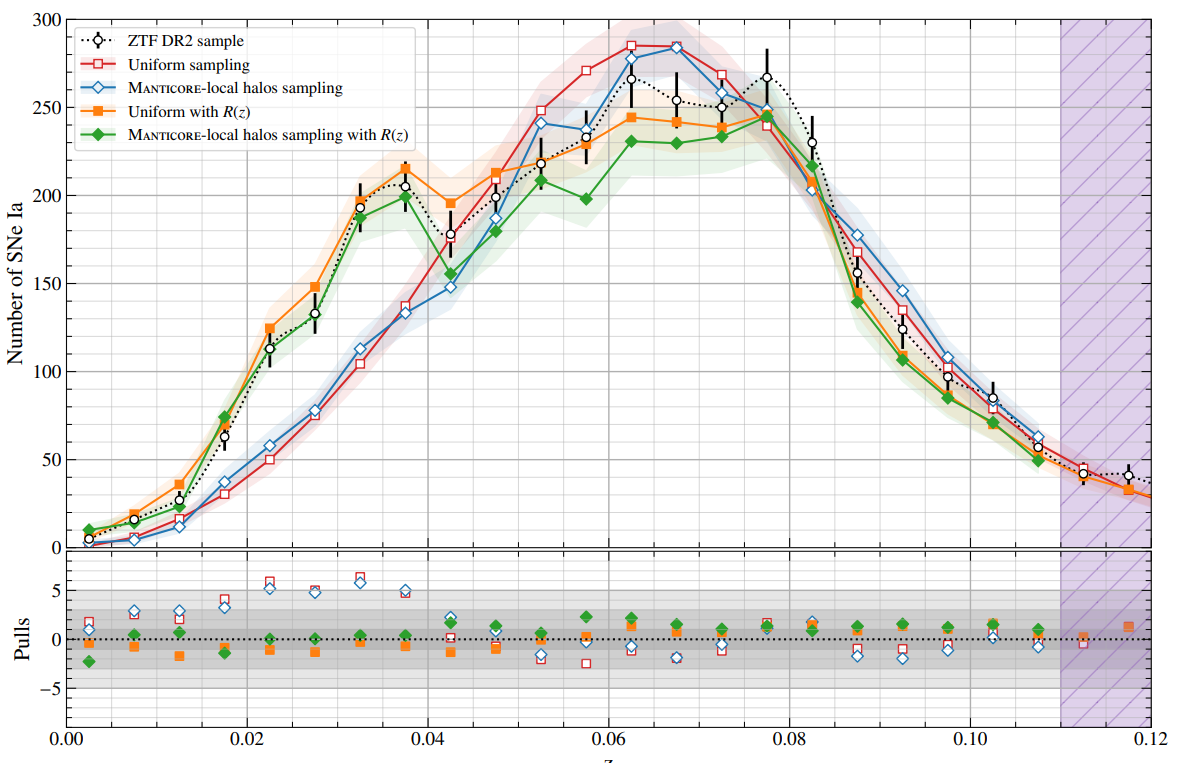
\includegraphics[width=0.8\textwidth]{MainLayout/Second_chapter/figures/sn_rate.png}
    \caption{Distribution of simulated supernova observed as a function of redshift $z$ vs the ZTF DR2 sample of obsereved supernovae (circle with black uncertainty). The different simulations are done using different priors on their positions. Red assumes a uniform sampling like \cite{Perley_2020}. Blue uses a uniform sampling weighted by halo masses from Manticore-local. Oragne assumes a redshift dependent rate. Green assumes a redshift dependent rate and weights by the halo masses.}
    \label{fig:sn_rate_antoine}
\end{figure}

\begin{figure}[ht]
    \centering
    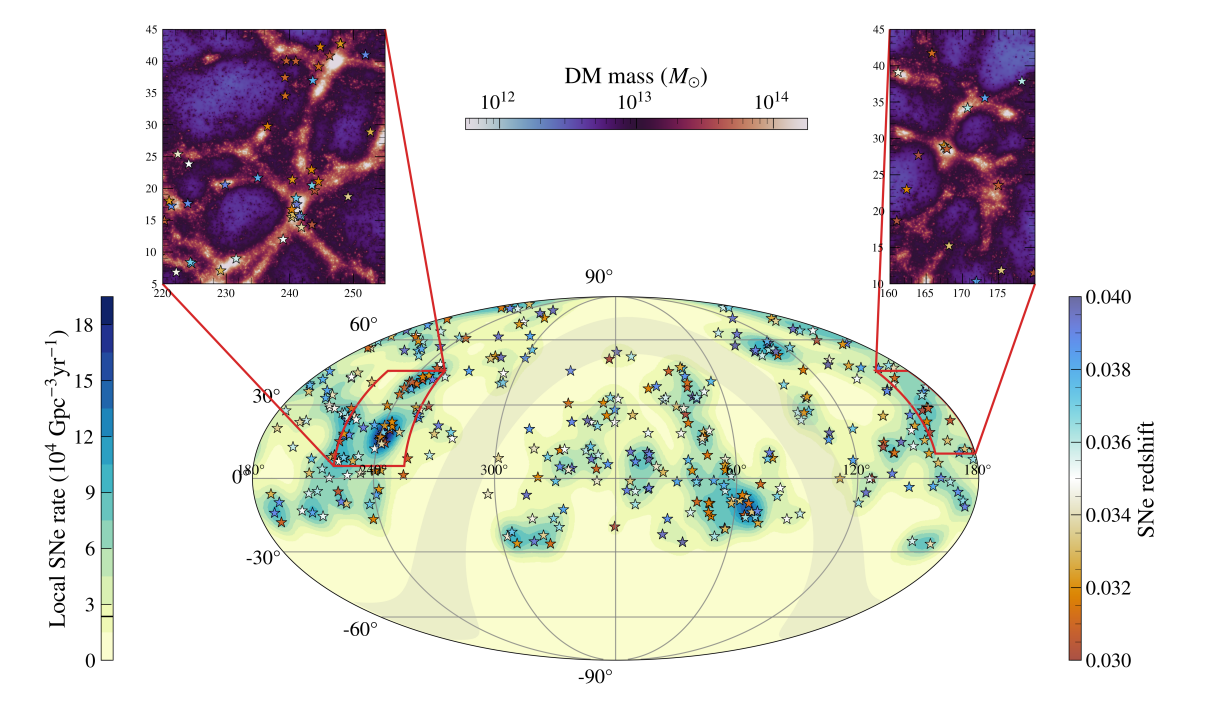
\includegraphics[width=1.0\textwidth]{MainLayout/Second_chapter/figures/sn_vs_delta.png}
    \caption{Distribution of supernova obsereved vs the dark matter distribution posterior from Manticore-local as well as the local supernova rate. Top left corner we have a zoom in on the Hercules supercluster. Top right corner we have a zoom in on the Leo supercluster.}
    \label{fig:sn_vs_delta_antoine}
\end{figure}

\subsection{Observations}

\noindent \textbf{\underline{Spectroscopic}} \\

Type Ia supernova spectra have a distinct spectra. Most of the light emitted from a type Ia is in the visible wavelengths with some parts of their spectra in the infrared and ultraviolet. 
During the initial phases of the explosion the external layers of the explosion are opaque. Near the maximum emission of light, we expect to see 
absoption lines of Silicium and Calcium caused by the fusion of Carbon and Oxygen. The days that follow, the opacity decreases and we start to see absoption lines 
from Nickel and Cobalt. Finally, in the following weeks the Nickel and Cobalt will disintegrate into Iron for which we see the absoption lines. \\

\begin{figure}[ht]
    \centering
    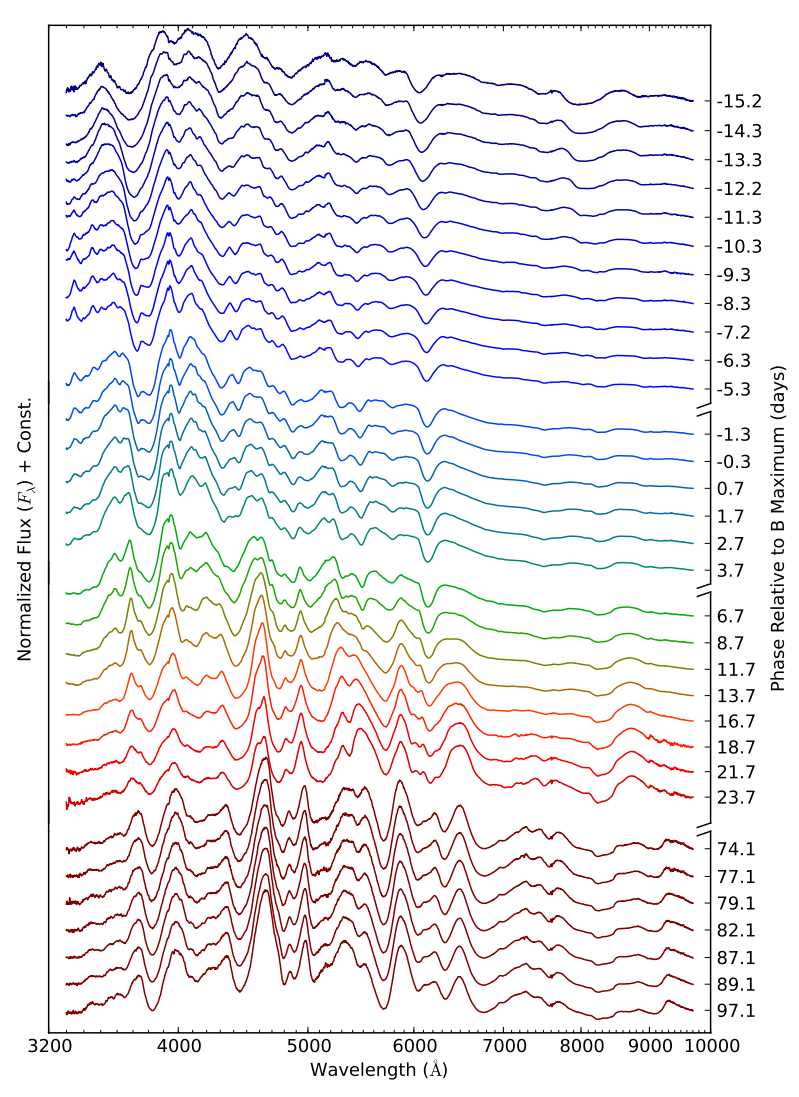
\includegraphics[width=0.7\textwidth]{MainLayout/Second_chapter/figures/sn2011fe_spectra_.png}
    \caption{Spectral series of SN 2011fe supernova taken by with the SNIFS instrument (\cite{Pereira_2013}). The spectra were captured betwenen -15 days to 50 days after the maximum emission data. They are ordered from top to bottom, or blue to red. The magnitude shown are relative to the maximum magnitude.}
    \label{fig:sn_spectra_2011fe}
\end{figure}

\noindent \textbf{\underline{Photometric}} \\

When describing the photometric evolution of type Ia supernovae, we are describing the integrated flux in a observation band or filter that covers a specific wavelength. Generally, 
we use the standard filters U, B, V, R and I (also known as the Bessel filters \cite{Bessell_1990}) that cover the ultraviolet, visible and near-infrared range.
We observe in all bands an increase the lightcurve that lasts approximately 20 days with an absolute magnitude in the B band of $-19.5$mag that occurs following the 
disintegration of Nickel. After that, the visible and ultraviolet bands measure an exponential decrease due to the disintegration into Iron. In the infrared bands, we observe 
a second peak somwhere between 20 to 25 days after the first peak. \\

\begin{figure}[ht]
    \centering
    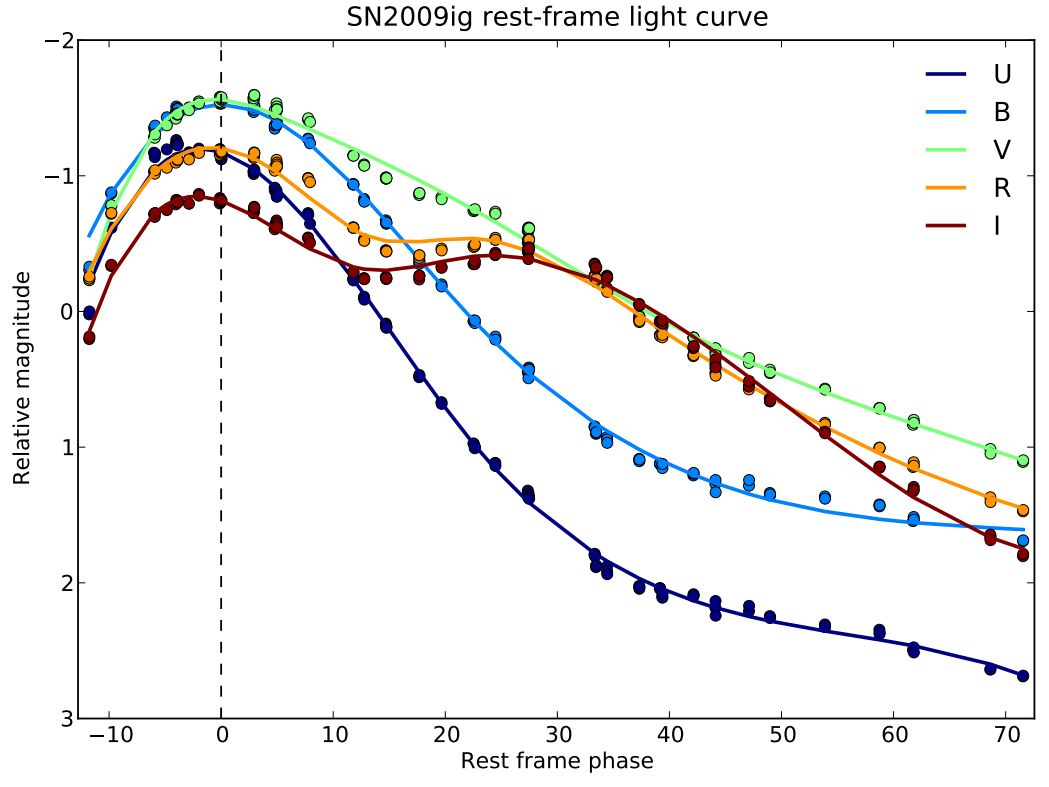
\includegraphics[width=0.7\textwidth]{MainLayout/Second_chapter/figures/sn2009ig_lightcurve.png}
    \caption{Synthetic lightcurves of the SN 2009ig supernova in the UBVRI bands made for the SNfactory collaboration taken from \cite{Chotard_2011}.}
    \label{fig:sn_lc_2009ig}
\end{figure}


\section{ZTF survey} \label{sec:ztf}
In this section we present the Zwicky Transient Facility survey as well as the the supernova sample that was primarily studied in this PhD the ZTF DR2. The ZTF camera is mounted on the Samuel Oschin 
48-inch (1.2m) telescope in the Mount Palomar Obsrevatory, California, USA. The primary purpose of the survey is the study of nearby astrophysical transients, which makes it 
really good for studying supernovae in the local Universe. \\

\begin{figure}[ht]
    \centering
    \includegraphics[width=1.0\textwidth]{MainLayout/Second_chapter/figures/palomar-observatory.jpg}
    \caption{Mount Palomar Observatory. Credits: Caltech \url{https://www.ztf.caltech.edu/} }
    \label{fig:palomar}
\end{figure}

\subsection{ZTF photometry}

The ZTF camera is made up of 16 CCDs (model e2v CCD231-C6) each possessing 6144 $\times$ 6160 pixels. The Samuel Oschin telescope contains a 1.2m mirror (called the "primary mirror" M1) that redirects the 
photons to the focal plane of the camera. The mirror is a spherical pyrex-glass mirror coated with aluminium which allows for a large observation field of view. 
The telescope also contains an aspherical lens at the entrance to correct for geometric aberrations. 
It covers a solid angle of $\sim 47 \text{deg}^2$ of the extragalactical northern sky and manages to conduct a full sky coverage twice per night. Each image covers approximately 235 times the area of the full moon. 
The photometry is done using 3 filters $g$, $r$ and $i$ covering the ranges of $\approx 4000 - 5500 \AA$, $\approx 5500 - 7000 \AA$ and $\approx 7000 - 9000 \AA$ respectively. 
It is important to highlight that the transmissions of the filters are sensor-dependent and we display them by averaging over the sensor transmissions. 
The magnitude limits for each band are $m_g \sim 20.8-21.1$mag, $m_r \sim 20.6-20.9$mag, $m_i \sim 19.9-20.2$mag where the variations are laregly due to the phases of the moon. 
The full details on the ZTF photometry are in \cite{Dekany_2020}. \\

\begin{figure}[ht]
    \centering
    \includegraphics[width=0.8\textwidth]{MainLayout/Second_chapter/figures/ztf-camera-fov.jpg}
    \caption{Comparisons between the fields of view of ZTF, PS1, LSST, PTF, SDSS and DES. In the background we see in comparison the size of the moon and the Andromeda galaxy. Credits: Caltech \url{https://www.ztf.caltech.edu/} }
    \label{fig:ztf_fov}
\end{figure}

\begin{figure}[ht]
    \centering
    \includegraphics[width=1.0\textwidth]{MainLayout/Second_chapter/figures/ztf_sn_picture.png}
    \caption{Type Ia supernova detected by ZTF. Photos taken accross 2 months (from left to right 20th of Jan 2020, 25th of Jan 2020, 7th of Feb 2020, 20th of Feb 2020, 20th of March 2020). Credits: Mikaël Rigault.}
    \label{fig:ztf_sn_picture}
\end{figure}

\begin{figure}[ht]
    \centering
    \includegraphics[width=0.8\textwidth]{MainLayout/Second_chapter/figures/ztf_cadence.png}
    \caption{ZTF cadence on the sky. Average number of visits per month for each field of ZTF in each band $g$, $r$ and $i$. Taken from \cite{Carres_2023}}
    \label{fig:ztf_cadence}
\end{figure}

\begin{figure}[ht]
    \centering
    \includegraphics[width=1.0\textwidth]{MainLayout/Second_chapter/figures/ztf_filters.pdf}
    \caption{ZTF filters. Dotted lines represent transmissions for different sensors. Solid lines represent the average transmissions over all sensors.}
    \label{fig:ztf_cadence}
\end{figure}

\subsection{Spectroscopic follow up}

ZTF is accompagnied by a spectrograph named the Spectral Energy Distribution Machine (SEDM) located in the same observatory on the P60 telescope. The purpose of the object to 
conduct a follow up on the photometry in order to properly classify the transients obsereved. It's limit magnitude is 20.5mag. This follow up played an important role in acquiring the 
60\% spectra for the ZTF Bright Transient Survey (BTS) for which the magnitude limit was 18.5mag, a limited fraction of the ZTF total survey. \\


\subsection{ZTF DR2}

We present in this subsection the type Ia supernova data release of ZTF named DR2. This encompasses data taken from March 2018 and December 2020. The sample contains 3628 
spectroscopically identified supernovae up to a redshift of $z \approx 0.2$. Figure \ref{fig:ztf_lcs} shows examples of the sampling of the supernova obsereved by ZTF in DR2. We must note that not all supernova data is 
"good" enough to be used for a cosmological analysis. For such an analysis, quality cuts on sampling around the maximum emission of light, the color and the stretch must be applied. 
The details on the cosmology quality cuts can be found in \cite{Rigault_2020} and we remind them later in Chapter 4. After the cuts, 
the sample maintains 2667 supernovae that pass. A subset of the sample named the "volume-limited" sample contains all supernovae up to a redshift of $z=0.06$ represents a complete 
sample of supernovae i.e. the sample is not influenced by any selection effects due to the magnitude limits of the telescope. This subset contains 994 supernovae. \\

\begin{figure}[ht]
    \centering
    \includegraphics[width=0.8\textwidth]{MainLayout/Second_chapter/figures/ztf_dr2_hubble.png}
    \caption{Hubble diagram created with standardized ZTF DR2 type Ia supernovae compared to fiducial $\Lambda$CDM cosmology anchore on Planck results. Taken from \cite{Rigault_2020}.}
    \label{fig:ztf_dr2_hubble}
\end{figure}

\begin{figure}[ht]
    \centering
    \includegraphics[width=0.5\textwidth]{MainLayout/Second_chapter/figures/ztf_sn_dr2.png}
    \caption{Three supernova Ia lightcurves examples highlighting the worst (top), average (middle) and best (bottom) sampling in DR2. The colors indicate the band they were measured in and the solid lines are the best SALT2 fits. Taken from \cite{Rigault_2020}}
    \label{fig:ztf_lcs}
\end{figure}



\section{DESI survey}

In this section, we briefly present the Dark Energy Spectroscopic Instrument (DESI). This novel, fully robotic instrument, has allowed us to observe the Universe in great detail and 
proven to being capable of adding insight to our understanding of the accelerated Universe (\cite{DESI_DR2_2025}). 
In april 2026, DESI completed its main observation sequence and covered $14000\text{deg}^2$ with over 60 million objects (with 47 million galaxies and quasars) observed within 5 years. \\

\subsection{Spectroscopic instrument}

DESI is a fourth-generation spectroscopic survey. It is a robotic fibre-fed spectroscopic instrument. 
It is installed on the 4-meter Mayall telescope at Kitt Peak National Observatory in Arizona, USA. 
It contains 5000 fibres, each able to observe a separate spectrum, allowing the instrument to gather 5000 spectra at a time, covering for one exposure around $3 \text{deg}^2$
part of the sky. This is a great improvement over its predecessor SDSS (\cite{Dawson_2016}) which had 1000 fibres positioned manually, therefore taking a lot more time than DESI. 
The DESI spectrograph covers a range of $3600-9800 \AA$ where the light is divided into three wavelength channels: Blue ($b$), Red ($r$) and Near Infrared ($Z$). Finally, the light 
is captured by CCDs installed in a vacuum cryostat. Two different CCD models are used: STA4150 (4096 $\times$ 4096 pixels) and CCDs produced by LBL specifically for DESI 
(4114 $\times$ 4128 pixels). More details on the instrument can be found here \cite{DESI_Instrument_2016}.\\

\subsection{Tracers}

DESI catalogues its observations under multiple classes each presenting a of matter tracer in the observable Universe (\cite{DESI_Design_2016}).

\noindent \textbf{\underline{BGS}} \\

The first catalogue is the Bright Galaxy Survey (BGS). It is a flux limited galaxy catalogue that is divided into two parts based in the magntidue of the obsereved galaxy. BGS 
Bright contains galaxies with magnitudes in the $r$ band $<19.5$ and BGS faint with magnitudes $19.5 - 20.175$, these are present at a redshift range of $z<0.6$. To identify if the obsereved object is a galaxy or a star it is 
cross references with the Gaia catalogue. If it is not present then it is a galaxy. There are over 10 million galaxies in the BGS catalogue. These also present the galaxies closest to us. \\

\noindent \textbf{\underline{LRG}} \\

The second catalogue is the Luminous Red Galaxies (LRG) which contains old elliptical galaxies, identified due the $4000\AA$ break line in their spectra, in which 
the star formation rate has stopped. The LRG present galaxies in the redshift range $0.4<z<1.0$.

\noindent \textbf{\underline{ELG}} \\

The third catalogue is the Emission Line Galaxies (ELG) which contains younger spiral galaxies with star formation. It is divided into two subcategories: ELG VLOP with galaxies 
at redshifts $0.6<z<1.1$ and ELG LOP with galaxies at $1.1<z<1.6$. \\ 

\noindent \textbf{\underline{QSO}} \\

The fourth catalogue is the Quasar-Stellar Objects (QSO). The catalogue contains quasars, active galactic nuclei which are powered by the accretion of super massive black holes. 
The quasars measured at a redshift of $0.9<z<2.1$ are used as direct matter tracers, while quasars at $2.1<z<4.0$ will be used for their Lyman-$\alpha$ forest. This 
represents the furthest objects obsereved by DESI. \\

DESI at the time of writing this thesis has entered an extension phase of observation until 2028 where the sky coverage will go up to $17000\text{deg}^2$. \\

\subsection{ZTF and DESI Synergies}

ZTF and DESI present two of the current generation surveys that will tackle known tensions in the cosmological model. In addition to that, ZTF's sky coverage is in fact encompassed 
by DESI's coverage and the BGS sample is actually present at the same redshift range as ZTF. This creates synergies between the surveys that could explored.\\ 
Firstly, DESI's spectroscopic instrument has more accurate measurements of redshifts than the SEDM, therefore redshifts provided by DESI to ZTF can improve 
the mapping of the expanding history of the Universe using supernovae. They will also provide more accurate measurements of growth rate of structures 
using ZTF since it heavily relies on comparing the observed redshift to the cosmological redshift due to the expansion (see Section \ref{sec:vp_methods}). \\ 
Secondly, the BGS Bright sample contains galaxies in the same redshift range as the ZTF DR2. This highly favours conducting cross-survey analyses, which is the main 
goal of this PhD regarding the measurement of the growth rate of structures $f\sigma_8$. The DESI growth rate of structure measurements at low redshift is limited by the cosmic 
variance (the statistical uncertainty that arises due to only having access to one realization of the Universe) and galaxy bias. Supernova measurements can directly probe 
the underlying velocity field (see Section \ref{sec:vp_methods}) independently of any galaxy bias. Therefore a combination of both DESI and ZTF is projected to yield more 
precise measurements of $f\sigma_8$ at a low redshift. This is particularly important since the measurement of the growth rate of structures is a direct test of GR and is most 
sensitive at low redshift. \\

\section{LEMAITRE: Hubble diagram project}

The LEMAITRE project aims at constructing the largest Hubble diagram by using an independent set of supernovae. One its objectives is to tackle the $(w_0-w_a)$ tension observed 
by recent results from \cite{Brout_2022}, \cite{Rubin_2023} and \cite{DES_2024} supernova analyses as well as the combination with BAO results from \cite{DESI_DR2_2025}. It is 
important to note that the low redshift supernova sample used in all three analyses is the same and that it seems to be the main motivating factor for the tension. 
By analyzing a completely new dataset for LEMAITRE, an independent assessment of this tension will be provided. Additionally with the LEMAITRE project comes a new 
analysis pipeline from end-to-end, starting from the lightcurve extraction and calibration up to the cosmological analysis. My work during the PhD involved the continued 
development and testing of a portion of the LEMAITRE pipeline named NaCl (see Chapter 3 and 4) which aims at training a spectrophotometric model. \\

\subsection{Datasets: ZTF, SNLS, HSC}

There are three datasets used in the LEMAITRE project: \\

\noindent \textbf{\underline{ZTF}} \\

The first will be the ZTF DR2 dataset making up the low-$z$ sample for the LEMAITRE analysis of about 2600 supernova. More details on the ZTF dataset and telescope are explained 
in \ref{sec:ztf}. \\

\noindent \textbf{\underline{SNLS}} \\

The second dataset is the SuperNova Legacy Survey (SNLS)  (Astier et al., 2006), a type Ia supernova survey conducted with the MegaCam (Boulade et al., 2003) observing system. 
The camera is mounted on the Canada-France-Hawaii 3.6m telescope (CFHT) located on top of the Maunakea volcano, Hawaii.
The focal plane of the MegaCam camera is made up of 40 CCDs (model e2v CCD42-90) each having 
2048 $\times$ 4612 pixels. The CFHT is constructed with two mirrors, the primary mirror has a parabolic shape and is made from a glass-ceramic
material which makes it immune to thermal distortion. The camera is placed in the focal plane of the primary mirror. In addition, a Wide Field
Corrector (WFC) is placed in front of the camera to guarantee a large field of view. \\ 

In order to classify observed supernovae and acquire their redshifts, 
a spectroscopic follow-up is implemented. These additional
observations mostly rely on the European Southern Observatory Very Large Telescope (ESOVLT), 
the Gemini-North and South and the Keck-I and II instruments (Balland et al., 2009;
Astier et al., 2006). As the photometric survey observes more type Ia candidates than what
can be spectroscopically observed afterwards, a target selection process must be implemented. 
In practice, a first light-curves fit is performed in real time which allows to eliminate most of the type II contamination in the survey
For the remaining targets, a limit of mi = 24.5mag (i-band magnitude) has been established, over which a supernova is less
likely to be spectroscopically observed.
The MegaCam camera footprint is a 0.96 × 0.94 = 0.90deg2
rectangle. As a consequence, the chosen observation strategy for SNLS is no longer a wide scan of a large fraction of the sky as for ZTF 
but rather consists is observing deeply (up to z  1) in four
dedicated fields equally distributed in right ascension (see figure 3.10 and table 3.1)
The luminosity of transients is collected through 5 photometric filters, g, r, i, i21
and z,
spanning the visible and near-infrared wavelength ranges. Figure 3.11 presents the transmission of the SNLS filters as a function of wavelength. 
As for ZTF earlier, we highlight the
fact that the transmissions are sensor-dependent by displaying the average transmission
over the focal plane and a transmission curve for four different sensors.
In this thesis, the analysed SNLS data consists in the five years survey (SNLS 5y), which
started in the second half of 2003 and ended in 2009. The dataset comprises SNLS 3y data
as well as data from the 4th and 5th years which will be published in Betoule et al. in prep.
Figure 3.12 presents the number of exposures per day as a function of time for the entire
SNLS survey. \\


\noindent \textbf{\underline{HSC}} \\


The Hyper Suprime-Cam Subaru Strategic Program (Aihara et al., 2022), also denoted HSCSSP, is an astronomical 
observation program which allocated some telescope time to the 
observation of type Ia supernovae at the end of the 2010’s. Its primary system is the Hyper
Suprime Cam, a camera mounted on the Subaru 8.2m telescope. As for the CFHT, the
Subaru telescope is located on top of the Maunakea volcano, Hawaii (see figure 3.13).
The focal plane of the Hyper Suprime-Cam camera includes 116 Hamamatsu CCDs 
each totalizing 2048 × 4096 = 8.4Mpx (Hyper Suprime Cam documentation). The Subaru
telescope also follows a Prime Focus architecture. Figure 3.14 presents a side view of the
Hyper Suprime Cam mounted on the Subaru telescope.
The redshifts of the HSC supernovae are determined by measuring the redshift of their
host galaxies. These redshifts were mainly collected by the AAT/AAOmega and DESI
instruments, completed by observations from the Subaru/FOCAS and VLT instruments
(Suzuki et al. in prep). As of today, around 500 redshifts have been measured and observations are still going on, in particular in the XMM field (see figure 3.15).
The HSC-SSP collaboration also developed four methods to determine the redshifts directly from photometry. The Direct Empirical Photometric method (DEmP) and the TPZ
method both rely on machine learning to infer redshifts. The first approach consists in
fitting a polynomial function modeling the redshift as a function of magnitude (Hsieh and
Yee, 2014) while the second one uses random forest algorithms (Carrasco Kind and Brunner,
2013). For complementary measurements, the LePhare and MIZUKI methods both relies on
template fitting with priors. While the LePhare approach uses redshift distributions priors
from the 30-band photometric redshifts of the COSMOS survey (Ilbert et al., 2009; Coupon
et al., 2015), the MIZUKI approach uses Bayesian priors (Tanaka, 2015). 
The Hyper Suprime-Cam camera footprint is a 1.8deg2 disc which is about twice the
size of the MegaCam footprint. Although the main focus of the HSC-SSP is to build a galaxy
catalog for weak lensing analysis, the observation cadence of its deep fields were adapted
for supernovae observation. Because the main goal of the HSC supernova survey is to
observe faint transients at high redshift (up to z  1.6), the chosen observation strategy
is also similar to SNLS. In fact, the supernovae observation is restricted to four dedicated
deep fields (XMM-LSS, E-COSMOS, ELAIS-N1, DEEP2-F3) and two ultra-deep fields (SXDS
and COSMOS), partially overlapping the SNLS D1 and D2 fields respectively. Figure 3.15
presents a summary of the HSC deep and ultra-deep fields locations. 
The luminosity of transients is collected through 7 photometric filters, g, r, r22
, i, i2, z
and y, spanning the visible and near-infrared wavelength ranges. Figure 3.16 presents the
transmission of the HSC filters as a function of wavelength. Although the transmissions are
sensor-dependent as for the ZTF and SNLS filters, we only display the average transmission
curves over the focal plane for clarity.

In this thesis, the analysed HSC data consists in the HSC supernova survey, which
started with a first observation season in 2017 and ended with a second observation season
in 2020. Figure 3.17 presents the number of exposures per day as a function of time for the
entire HSC survey

\subsection{Pipeline overview}
\subsection{Cosmological analyses with LEMAITRE}
\subsection{Uncertainties in SN measurements?}

\section{Peculiar velocities} \label{sec:vp_methods}
\subsection{Extracting peculiar velocities}
\subsection{Growth rate of structures}
\subsubsection{Maximum likelihood fields}

 - Uses covariances between velocities in a likelihood \\
 - velocities modeled before hand \\
 - maximize the likelihood \\

\subsubsection{Compressed two-point statistics}

 - Uses covariances between velocities binned \\
 - Defines correlation function and power spectrum \\
 - Modelling power spectra contains cosmological information \\

\subsubsection{Density field reconstruction}

 - Uses velocities from galaxies/ SN \\
 - Reconstruct from the velocities the current density field \\

\subsubsection{Field level forward modeling}

 - Model initial density field and evolve it based on a gravity model \\
 - Fit initial field and cosmological parameters \\



\chapter{\textsc{Lemaître} project}\label{chap3}
\minitoc 
\section{LEMAITRE: Hubble diagram project overview}

The LEMAITRE project aims at constructing the largest Hubble diagram by using an independent set of supernovae. One its objectives is to tackle the $(w_0-w_a)$ tension observed 
by recent results from \cite{Brout_2022}, \cite{Rubin_2023} and \cite{DES_2024} supernova analyses as well as the combination with BAO results from \cite{DESI_DR2_2025}. It is 
important to note that the low redshift supernova sample used in all three analyses is the same and that it seems to be the main motivating factor for the tension. 
By analyzing a completely new dataset for LEMAITRE, an independent assessment of this tension will be provided. Additionally with the LEMAITRE project comes a new 
analysis pipeline from end-to-end, starting from the lightcurve extraction and calibration up to the cosmological analysis. My work during the PhD involved the continued 
development and testing of a portion of the LEMAITRE pipeline named NaCl (see Chapter 3 and 4) which aims at training a spectrophotometric model. \\

\section{Datasets: ZTF, SNLS, HSC}

There are three datasets used in the LEMAITRE project: \\

\subsection{ZTF survey} \label{sec:ztf}
In this section we present the Zwicky Transient Facility survey as well as the the supernova sample that was primarily studied in this PhD the ZTF DR2. The ZTF camera is mounted on the Samuel Oschin 
48-inch (1.2m) telescope in the Mount Palomar Obsrevatory, California, USA. The primary purpose of the survey is the study of nearby astrophysical transients, which makes it 
really good for studying supernovae in the local Universe. \\

\begin{figure}[ht]
    \centering
    \includegraphics[width=1.0\textwidth]{MainLayout/Third_chapter/figures/palomar-observatory.jpg}
    \caption{Mount Palomar Observatory. Credits: Caltech \url{https://www.ztf.caltech.edu/} }
    \label{fig:palomar}
\end{figure}

\subsubsection{ZTF photometry}

The ZTF camera is made up of 16 CCDs (model e2v CCD231-C6) each possessing 6144 $\times$ 6160 pixels. The Samuel Oschin telescope contains a 1.2m mirror (called the "primary mirror" M1) that redirects the 
photons to the focal plane of the camera. The mirror is a spherical pyrex-glass mirror coated with aluminium which allows for a large observation field of view. 
The telescope also contains an aspherical lens at the entrance to correct for geometric aberrations. 
It covers a solid angle of $\sim 47 \text{deg}^2$ of the extragalactical northern sky and manages to conduct a full sky coverage twice per night. Each image covers approximately 235 times the area of the full moon. 
The photometry is done using 3 filters $g$, $r$ and $i$ covering the ranges of $\approx 4000 - 5500 \AA$, $\approx 5500 - 7000 \AA$ and $\approx 7000 - 9000 \AA$ respectively. 
It is important to highlight that the transmissions of the filters are sensor-dependent and we display them by averaging over the sensor transmissions. 
The magnitude limits for each band are $m_g \sim 20.8-21.1$mag, $m_r \sim 20.6-20.9$mag, $m_i \sim 19.9-20.2$mag where the variations are laregly due to the phases of the moon. 
The full details on the ZTF photometry are in \cite{Dekany_2020}. \\

\begin{figure}[ht]
    \centering
    \includegraphics[width=0.8\textwidth]{MainLayout/Third_chapter/figures/ztf-camera-fov.jpg}
    \caption{Comparisons between the fields of view of ZTF, PS1, LSST, PTF, SDSS and DES. In the background we see in comparison the size of the moon and the Andromeda galaxy. Credits: Caltech \url{https://www.ztf.caltech.edu/} }
    \label{fig:ztf_fov}
\end{figure}

\begin{figure}[ht]
    \centering
    \includegraphics[width=1.0\textwidth]{MainLayout/Third_chapter/figures/ztf_sn_picture.png}
    \caption{Type Ia supernova detected by ZTF. Photos taken accross 2 months (from left to right 20th of Jan 2020, 25th of Jan 2020, 7th of Feb 2020, 20th of Feb 2020, 20th of March 2020). Credits: Mikaël Rigault.}
    \label{fig:ztf_sn_picture}
\end{figure}

\begin{figure}[ht]
    \centering
    \includegraphics[width=0.8\textwidth]{MainLayout/Third_chapter/figures/ztf_cadence.png}
    \caption{ZTF cadence on the sky. Average number of visits per month for each field of ZTF in each band $g$, $r$ and $i$. Taken from \cite{Carres_2023}}
    \label{fig:ztf_cadence}
\end{figure}

\begin{figure}[ht]
    \centering
    \includegraphics[width=1.0\textwidth]{MainLayout/Third_chapter/figures/ztf_filters.pdf}
    \caption{ZTF filters. Dotted lines represent transmissions for different sensors. Solid lines represent the average transmissions over all sensors.}
    \label{fig:ztf_cadence}
\end{figure}

\subsubsection{Spectroscopic follow up}

ZTF is accompagnied by a spectrograph named the Spectral Energy Distribution Machine (SEDM) located in the same observatory on the P60 telescope. The purpose of the object to 
conduct a follow up on the photometry in order to properly classify the transients obsereved. It's limit magnitude is 20.5mag. This follow up played an important role in acquiring the 
60\% spectra for the ZTF Bright Transient Survey (BTS) for which the magnitude limit was 18.5mag, a limited fraction of the ZTF total survey. \\


\subsubsection{ZTF DR2}

We present in this subsection the type Ia supernova data release of ZTF named DR2. This encompasses data taken from March 2018 and December 2020. The sample contains 3628 
spectroscopically identified supernovae up to a redshift of $z \approx 0.2$. Figure \ref{fig:ztf_lcs} shows examples of the sampling of the supernova obsereved by ZTF in DR2. We must note that not all supernova data is 
"good" enough to be used for a cosmological analysis. For such an analysis, quality cuts on sampling around the maximum emission of light, the color and the stretch must be applied. 
The details on the cosmology quality cuts can be found in \cite{Rigault_2020} and we remind them later in Chapter 4. After the cuts, 
the sample maintains 2667 supernovae that pass. A subset of the sample named the "volume-limited" sample contains all supernovae up to a redshift of $z=0.06$ represents a complete 
sample of supernovae i.e. the sample is not influenced by any selection effects due to the magnitude limits of the telescope. This subset contains 994 supernovae. \\

\begin{figure}[ht]
    \centering
    \includegraphics[width=0.8\textwidth]{MainLayout/Third_chapter/figures/ztf_dr2_hubble.png}
    \caption{Hubble diagram created with standardized ZTF DR2 type Ia supernovae compared to fiducial $\Lambda$CDM cosmology anchore on Planck results. Taken from \cite{Rigault_2020}.}
    \label{fig:ztf_dr2_hubble}
\end{figure}

\begin{figure}[ht]
    \centering
    \includegraphics[width=0.5\textwidth]{MainLayout/Third_chapter/figures/ztf_sn_dr2.png}
    \caption{Three supernova Ia lightcurves examples highlighting the worst (top), average (middle) and best (bottom) sampling in DR2. The colors indicate the band they were measured in and the solid lines are the best SALT2 fits. Taken from \cite{Rigault_2020}}
    \label{fig:ztf_lcs}
\end{figure}


\subsection{SNLS survey} \label{sec:snls}

The second dataset is the SuperNova Legacy Survey (SNLS)  (Astier et al., 2006), a type Ia supernova survey conducted with the MegaCam (Boulade et al., 2003) observing system. 
The camera is mounted on the Canada-France-Hawaii 3.6m telescope (CFHT) located on top of the Maunakea volcano, Hawaii.
The focal plane of the MegaCam camera is made up of 40 CCDs (model e2v CCD42-90) each having 
2048 $\times$ 4612 pixels. The CFHT is constructed with two mirrors, the primary mirror has a parabolic shape and is made from a glass-ceramic
material which makes it immune to thermal distortion. The camera is placed in the focal plane of the primary mirror. In addition, a Wide Field
Corrector (WFC) is placed in front of the camera to guarantee a large field of view. \\ 

In order to classify observed supernovae and acquire their redshifts, 
a spectroscopic follow-up is implemented. These additional
observations mostly rely on the European Southern Observatory Very Large Telescope (ESOVLT), 
the Gemini-North and South and the Keck-I and II instruments (Balland et al., 2009;
Astier et al., 2006). As the photometric survey observes more type Ia candidates than what
can be spectroscopically observed afterwards, a target selection process must be implemented. 
In practice, a first light-curves fit is performed in real time which allows to eliminate most of the type II contamination in the survey
For the remaining targets, a limit of mi = 24.5mag (i-band magnitude) has been established, over which a supernova is less
likely to be spectroscopically observed.
The MegaCam camera footprint is a 0.96 × 0.94 = 0.90deg2
rectangle. As a consequence, the chosen observation strategy for SNLS is no longer a wide scan of a large fraction of the sky as for ZTF 
but rather consists is observing deeply (up to z  1) in four
dedicated fields equally distributed in right ascension (see figure 3.10 and table 3.1)
The luminosity of transients is collected through 5 photometric filters, g, r, i, i21
and z,
spanning the visible and near-infrared wavelength ranges. Figure 3.11 presents the transmission of the SNLS filters as a function of wavelength. 
As for ZTF earlier, we highlight the
fact that the transmissions are sensor-dependent by displaying the average transmission
over the focal plane and a transmission curve for four different sensors.
In this thesis, the analysed SNLS data consists in the five years survey (SNLS 5y), which
started in the second half of 2003 and ended in 2009. The dataset comprises SNLS 3y data
as well as data from the 4th and 5th years which will be published in Betoule et al. in prep.
Figure 3.12 presents the number of exposures per day as a function of time for the entire
SNLS survey. \\


\subsection{HSC survey} \label{sec:hsc}


The Hyper Suprime-Cam Subaru Strategic Program (Aihara et al., 2022), also denoted HSCSSP, is an astronomical 
observation program which allocated some telescope time to the 
observation of type Ia supernovae at the end of the 2010’s. Its primary system is the Hyper
Suprime Cam, a camera mounted on the Subaru 8.2m telescope. As for the CFHT, the
Subaru telescope is located on top of the Maunakea volcano, Hawaii (see figure 3.13).
The focal plane of the Hyper Suprime-Cam camera includes 116 Hamamatsu CCDs 
each totalizing 2048 × 4096 = 8.4Mpx (Hyper Suprime Cam documentation). The Subaru
telescope also follows a Prime Focus architecture. Figure 3.14 presents a side view of the
Hyper Suprime Cam mounted on the Subaru telescope.
The redshifts of the HSC supernovae are determined by measuring the redshift of their
host galaxies. These redshifts were mainly collected by the AAT/AAOmega and DESI
instruments, completed by observations from the Subaru/FOCAS and VLT instruments
(Suzuki et al. in prep). As of today, around 500 redshifts have been measured and observations are still going on, in particular in the XMM field (see figure 3.15).
The HSC-SSP collaboration also developed four methods to determine the redshifts directly from photometry. The Direct Empirical Photometric method (DEmP) and the TPZ
method both rely on machine learning to infer redshifts. The first approach consists in
fitting a polynomial function modeling the redshift as a function of magnitude (Hsieh and
Yee, 2014) while the second one uses random forest algorithms (Carrasco Kind and Brunner,
2013). For complementary measurements, the LePhare and MIZUKI methods both relies on
template fitting with priors. While the LePhare approach uses redshift distributions priors
from the 30-band photometric redshifts of the COSMOS survey (Ilbert et al., 2009; Coupon
et al., 2015), the MIZUKI approach uses Bayesian priors (Tanaka, 2015). 
The Hyper Suprime-Cam camera footprint is a 1.8deg2 disc which is about twice the
size of the MegaCam footprint. Although the main focus of the HSC-SSP is to build a galaxy
catalog for weak lensing analysis, the observation cadence of its deep fields were adapted
for supernovae observation. Because the main goal of the HSC supernova survey is to
observe faint transients at high redshift (up to z  1.6), the chosen observation strategy
is also similar to SNLS. In fact, the supernovae observation is restricted to four dedicated
deep fields (XMM-LSS, E-COSMOS, ELAIS-N1, DEEP2-F3) and two ultra-deep fields (SXDS
and COSMOS), partially overlapping the SNLS D1 and D2 fields respectively. Figure 3.15
presents a summary of the HSC deep and ultra-deep fields locations. 
The luminosity of transients is collected through 7 photometric filters, g, r, r22
, i, i2, z
and y, spanning the visible and near-infrared wavelength ranges. Figure 3.16 presents the
transmission of the HSC filters as a function of wavelength. Although the transmissions are
sensor-dependent as for the ZTF and SNLS filters, we only display the average transmission
curves over the focal plane for clarity.

In this thesis, the analysed HSC data consists in the HSC supernova survey, which
started with a first observation season in 2017 and ended with a second observation season
in 2020. Figure 3.17 presents the number of exposures per day as a function of time for the
entire HSC survey

\subsection{Pipeline overview}
\subsection{Cosmological analyses with LEMAITRE}
\subsection{Uncertainties in SN measurements?}

\section{Pipeline}


\subsection{Pipeline overview}
\subsection{Cosmological analyses with LEMAITRE}
\subsection{Uncertainties in SN measurements?}

\section{LEMAÎTRE Data Challenges}

In this section we will be detailing the LEMAÎTRE Data Challenges, DCs from now on. The goal of these challenges is to validate the new analysis pipeline that is part of the LEMAÎTRE project, which is an extremely important key test before running the full analysis chain on the real data.

\subsection{General description of the DCs}

The LEMAÎTRE analysis pipeline is brand new from the point where the lightcurves are extracted from the ZTF, SNLS and HSC surveys up until comsological parameters are determined. The pipeline can be divided into 2 main parts : the lightcurve extraction and calibration pipeline, and the Georges pipline (or the cosmological analysis pipeline). Determining whether this new pipeline can accurately predict cosmological parameters without any biases is crucial and must be investigated thoroughly, especially since many of the elements of the pipeline depend on each other. \\
We will be focused here on the validity of the cosmological analysis pipeline, Georges. For that, the pipeline will face a series of challenges, each with an increasing level of complexity representing a challenge we are expected to face in the final analysis on the LEMAÎTRE dataset. Those challenges are the DCs and they are constituted of realistic simulations of ZTF, SNLS and HSC lightcurves and spectra. We will firstly describe the different elements of the Georges pipeline and then the different elements of the DCs. Each DC is constituted of 100 realizations of the simulations, essentially containing the exact same supernova but by applying the noise on the data differently. This will allow us to perform a robust coverage test for each DC.

\subsection{Georges analysis pipeline}

The Georges pipeline consists of mainly four modules : PeTS, NaCl, EDRIS, cosmologix.

\subsubsection{PeTS \& miniPeTS}

\noindent \textbf{\underline{PeTS}} \\


The PeTS module aims at "cleaning" the training dataset we will ll be using in the cosmological analysis. The reason we need to do that is because some of the supernova lightcurves can contain issues such as few points, very noisy data or a mix of both that can introduce issues when trying to accurately model the supernova with NaCl.\\

In order to avoid that, PeTS applies a set of data quality cuts that will ensure that we select a subset on which we will be able to properly measure all of the supernova parameters.\\
The selection will be applied on supernovae that meets the following criteria:
\begin{itemize}
    \item The date of maximum emission ($t_{max}$) needs to be properly defined
    \item The color and the stretch parameters need to be accurately measured
    \item The supernova must contain at least 5 points with an SNR superior to 3, present in 2 bands and present within 50 days of the initial guess of $t_{max}$
\end{itemize}

In order to do that, PeTS initially fits all of the lightcurves with the SALT2.4 model using sncosmo (\cite{sncosmo}). \textbf{The sncosmo fit needs to converge in order to select a supernova in our final dataset}. That initial fit allows us to have an initial guess on the parameters $c$, $X_1$ and $t_{max}$. \\
The next thing is to create a log-likelihood profile while varying the value of $t_{max}$. The supernova is then selected if the following criteria are met on the parameter $t_{max}$:
\begin{itemize}
    \item The uncertainty on $t_{max}$ derived from the log-likelihood profile must be inferior to 1 day
    \item The log-likelihood profile must be symmetric. The condition chosen for that in PeTS is : $$|3\sigma(t_{max})_{Left} - 3\sigma(t_{max})_{Right}| < 0.3$$
    \item The log likelihood profile must present only 1 minimum within $3\sigma$
\end{itemize}
Lastly, the uncertainties on $c$ and $X_1$ need to be inferior to 0.3 and 1.\\

\noindent If all of these conditions are met, the supernova will be present in the final dataset. For the DCs, we want to apply PeTS on only 1 realization since the quality cuts shouldn't vary between realizations. Running PeTS, however, presents a difficulty. Creating the log-likelihood profile for each supernova takes a lot of computational time. It would take us a really long to do so if we wanted to perform multiple tests on any DC. In order to avoid that and gain a bit of time, we introduced miniPeTS.\\

\noindent \textbf{\underline{miniPeTS}} \\
With miniPeTS the goal is to achieve similar quality cuts to PeTS but much faster. This means that we don't expect to necessarily obtain the best quality dataset, but good enough to test the pipeline on the DCs. We apply similar cuts to the ZTF DR2 cuts (ref). We can summarize the quality cuts done with miniPeTS in the following list: 
\begin{itemize}
    \item The supernova needs to be measured in at least 2 bands
    \item The supernova needs to have at least 5 total measurements
    \item The supernova needs to have at least 2 measurement points before $t_{max}$
    \item The supernova needs to have at least 2 measurement points after $t_{max}$
    \item $-0.2<c<0.8$
    \item $|X_1|<3$
    \item SNLS and HSC supernova need to be measured at $z>0.2$
    \item $E(B-V)_{MW}<0.25$
\end{itemize}

\subsubsection{Data compression}

Before we can start training a model with NaCl on the data, we decided to accelerate the training by compressing the data on the basis of the model.

\noindent \textbf{\underline{Lightcurve compression}} \\

The way we compress the lightcurves data is by averaging the fluxes measured per night. We find that doing so reduces the size of lightcurves files by almost half.\\

\noindent \textbf{\underline{Spectra compression}} \\

We have also noticed that the resolution of the spectra is much higher than the resolution of our model. The spatial dimension of our model in NaCl is defined by a B-spline basis of order 4. Projecting the spectra on that basis can be written as 
$$ \sum_i p_i\mathcal{B}_i(\lambda) $$
The idea is retain the $p_i$ parameters alongside their uncertainties. The size of the spectral data is then reduced by a factor of 10.

\subsubsection{NaCl}

The next step in the Georges analysis pipeline is the model training with NaCl. The $X_0$, $X_1$ and $c$ along with the marginalized covariance matrix will be the input for EDRIS in order to estimate the supernova distances.

\subsubsection{EDRIS}

The observed distance modulus of type Ia supernova contains a natural dispersion with respect the Hubble law of around $\sim0.4 \mathrm{mag}$. This can be reduced by standardizing the distance moudli. We commonly use the Tripp relation (ref) which reduces this dispersion to $\sim0.15\mathrm{mag}$. It is expressed as follows : 

\begin{equation}
    \mu = m_B - (M_B - \alpha X_1 + \beta c)
    \label{eqn:tripp}
\end{equation}

\begin{equation}
    m_B = -2.5\log_{10}(X_0)
    \label{eqn:mb}
\end{equation}

with $m_B$ being the observed magnitude, $M_B$ the absolute magnitude and ($\alpha$, $\beta$) are the standardization parameters also known as the brighter slower and brighter bluer parameters. This is due to the fact that type Ia supernova with a larger stretch parameter tend to be brighter as well as supernova that are bluer.\\
The remaining $0.15\mathrm{mag}$ dispersion are due an intrinsic variability between supernovae that isn't modeled by the Tripp relation. \\

Determining the standardized parameters can be difficult. Since telescopes can only observe objects up to a certain magnitude we expect a cutoff in magnitude for each survey. Coupled with the intrinsic dispersion of supernova, this means that the population of supernova observed by a survey will skewed, favoring redder and faster supernova. We call this \textbf{selection effects}. This makes a direct determination of ($\alpha, \beta$) biased and will bias any cosmological analysis.\\

The goal of EDRIS is to accurately estimate unbiased standardized distances for complete and incomplete supernova Ia samples. EDRIS takes as input the parameters from NaCl alongside their covariance matrix, and will use that to infer standardization parameters ($\alpha$, $\beta$), $M_B$, selection effects and the intrinsic dispersion denoted $\sigma_{int}$.\\

\subsubsection{Cosmologix}

The final step of the pipeline is to infer the cosmological parameters from the distances and we do that with cosmologix \footnote{\url{https://lemaitre.pages.in2p3.fr/cosmologix/home.html}}  (Betoule et al in review), a fast JAX-coded software designed to accurately infer cosmological parameters. It is also possible to combine the supernova results with other probes such as BAO and CMB. This will be useful in the analysis of the real data.\\

\subsection{DC1}

The first data challenge will be a consistency test for the full chain. It's the first time we've tested the full pipeline together on the same dataset. This will also serve as a stepping stone for the analysis of the future DCs since they will be incrementing layers of complexity on top of what was done in DC1. We will be including simulated lightcurves and spectra from ZTF and SNLS as well as lightcurves from HSC.\\

The simulated data will include measurement uncertainties, an error snake and an intrinsic dispersion. We will not be including any selection effects so EDRIS will need to find the standardization parameters. The main challenge will be for NaCl to ensure that training the model with our current model constraints and regularization on a LEMAÎTRE like dataset does not bias our cosmological analysis.\\

The metric used to determine if we have passed the DC or not will be to check the coverage for the cosmological parameters after 100 realizations and ensuring it stays within $1 \sigma$.

\subsection{DC2}

The second data challenge serves as a test to the model selection effects in EDRIS. The simulations will be identical to DC1 with the addition of a selection function for each survey.\\

The metric used to determine if we have passed the DC or not will be the same as DC1.\\

\subsection{DC3}

In the third data challenge, calibration uncertainties and supernova outliers will be added the simulation. This serves as a main test to NaCl's error model to see how well it can identify outliers as well as determining the impact of calibration uncertainties on the reconstructed cosmology. \\

The metric used to determine if we have passed the DC or not will be the same as DC1 and DC2. \\

\subsection{DC4}

In the fourth data challenge, the simulations will include as many realistic effects as possible adding all sources of uncertainties and systematics that we know can affect our analysis. This includes realistic distributions of the stretch and color (ref madeleine), non type Ia contamination, astrophysical effects and color scatter effects. This will be a challenge for both NaCl and EDRIS. \\

The metric we will use here to determine if we have passed the DC or not will be the same as before. Since astrophysical effects aren't directly taken into account during the modeling of type Ia supernova, we will quantifying its effects on the reconstructed cosmology and see how we can minimize it.\\

\subsection{DC5}

In the fifth and final DC we will be placing ourselves in the same conditions of the realistic simulations by blinding the data. The party that will be blinding the data will not be the same as the one running the pipeline simulation. The goal is to obtain the correct cosmological parameters after unblinding the data. \\

We can summarize the DCs in the following diagram : \\

\begin{tikzpicture}[
    node distance=1.5cm and 1cm,
    every node/.style={draw, minimum width=2.3cm, minimum height=1cm, align=center},
    arrow/.style={-Stealth, thick}
]

% Define nodes
\node (DC1) {DC1};
\node[right=of DC1] (DC2) {DC2};
\node[right=of DC2] (DC3) {DC3};
\node[right=of DC3] (DC4) {DC4};
\node[right=of DC4] (DC5) {DC5};

\node[below=1.cm of DC1] (A) {Consistency of \\ the analysis \\ chain and \\ description \\ of the data};
\node[below=1.cm of DC2] (B) {Selection\\ effects};
\node[below=1.cm of DC3] (C) {Calibration \\ uncertainties and \\ outliers};
\node[below=1.cm of DC4] (D) {Color scatter \\ effects and \\ astrophysical \\effects};
\node[below=1.cm of DC5] (E) {Blinding the \\ data};

% Arrows between DCs
\draw[arrow] (DC1) -- (DC2);
\draw[arrow] (DC2) -- (DC3);
\draw[arrow] (DC3) -- (DC4);
\draw[arrow] (DC4) -- (DC5);

% Arrows down to tasks
\draw[arrow] (DC1) -- (A);
\draw[arrow] (DC2) -- (B);
\draw[arrow] (DC3) -- (C);
\draw[arrow] (DC4) -- (D);
\draw[arrow] (DC5) -- (E);

\end{tikzpicture}

%
\section{DESI survey}

In this section, we briefly present the Dark Energy Spectroscopic Instrument (DESI). This novel, fully robotic instrument, has allowed us to observe the Universe in great detail and 
proven to being capable of adding insight to our understanding of the accelerated Universe (\cite{DESI_DR2_2025}). 
In april 2026, DESI completed its main observation sequence and covered $14000\text{deg}^2$ with over 60 million objects (with 47 million galaxies and quasars) observed within 5 years. \\

\subsection{Spectroscopic instrument}

DESI is a fourth-generation spectroscopic survey. It is a robotic fibre-fed spectroscopic instrument. 
It is installed on the 4-meter Mayall telescope at Kitt Peak National Observatory in Arizona, USA. 
It contains 5000 fibres, each able to observe a separate spectrum, allowing the instrument to gather 5000 spectra at a time, covering for one exposure around $3 \text{deg}^2$
part of the sky. This is a great improvement over its predecessor SDSS (\cite{Dawson_2016}) which had 1000 fibres positioned manually, therefore taking a lot more time than DESI. 
The DESI spectrograph covers a range of $3600-9800 \AA$ where the light is divided into three wavelength channels: Blue ($b$), Red ($r$) and Near Infrared ($Z$). Finally, the light 
is captured by CCDs installed in a vacuum cryostat. Two different CCD models are used: STA4150 (4096 $\times$ 4096 pixels) and CCDs produced by LBL specifically for DESI 
(4114 $\times$ 4128 pixels). More details on the instrument can be found here \cite{DESI_Instrument_2016}.\\

\subsection{Tracers}

DESI catalogues its observations under multiple classes each presenting a of matter tracer in the observable Universe (\cite{DESI_Design_2016}).

\noindent \textbf{\underline{BGS}} \\

The first catalogue is the Bright Galaxy Survey (BGS). It is a flux limited galaxy catalogue that is divided into two parts based in the magntidue of the obsereved galaxy. BGS 
Bright contains galaxies with magnitudes in the $r$ band $<19.5$ and BGS faint with magnitudes $19.5 - 20.175$, these are present at a redshift range of $z<0.6$. To identify if the obsereved object is a galaxy or a star it is 
cross references with the Gaia catalogue. If it is not present then it is a galaxy. There are over 10 million galaxies in the BGS catalogue. These also present the galaxies closest to us. \\

\noindent \textbf{\underline{LRG}} \\

The second catalogue is the Luminous Red Galaxies (LRG) which contains old elliptical galaxies, identified due the $4000\AA$ break line in their spectra, in which 
the star formation rate has stopped. The LRG present galaxies in the redshift range $0.4<z<1.0$.

\noindent \textbf{\underline{ELG}} \\

The third catalogue is the Emission Line Galaxies (ELG) which contains younger spiral galaxies with star formation. It is divided into two subcategories: ELG VLOP with galaxies 
at redshifts $0.6<z<1.1$ and ELG LOP with galaxies at $1.1<z<1.6$. \\ 

\noindent \textbf{\underline{QSO}} \\

The fourth catalogue is the Quasar-Stellar Objects (QSO). The catalogue contains quasars, active galactic nuclei which are powered by the accretion of super massive black holes. 
The quasars measured at a redshift of $0.9<z<2.1$ are used as direct matter tracers, while quasars at $2.1<z<4.0$ will be used for their Lyman-$\alpha$ forest. This 
represents the furthest objects obsereved by DESI. \\

DESI at the time of writing this thesis has entered an extension phase of observation until 2028 where the sky coverage will go up to $17000\text{deg}^2$. \\

\subsection{ZTF and DESI Synergies}

ZTF and DESI present two of the current generation surveys that will tackle known tensions in the cosmological model. In addition to that, ZTF's sky coverage is in fact encompassed 
by DESI's coverage and the BGS sample is actually present at the same redshift range as ZTF. This creates synergies between the surveys that could explored.\\ 
Firstly, DESI's spectroscopic instrument has more accurate measurements of redshifts than the SEDM, therefore redshifts provided by DESI to ZTF can improve 
the mapping of the expanding history of the Universe using supernovae. They will also provide more accurate measurements of growth rate of structures 
using ZTF since it heavily relies on comparing the observed redshift to the cosmological redshift due to the expansion (see Section \ref{sec:vp_methods}). \\ 
Secondly, the BGS Bright sample contains galaxies in the same redshift range as the ZTF DR2. This highly favours conducting cross-survey analyses, which is the main 
goal of this PhD regarding the measurement of the growth rate of structures $f\sigma_8$. The DESI growth rate of structure measurements at low redshift is limited by the cosmic 
variance (the statistical uncertainty that arises due to only having access to one realization of the Universe) and galaxy bias. Supernova measurements can directly probe 
the underlying velocity field (see Section \ref{sec:vp_methods}) independently of any galaxy bias. Therefore a combination of both DESI and ZTF is projected to yield more 
precise measurements of $f\sigma_8$ at a low redshift. This is particularly important since the measurement of the growth rate of structures is a direct test of GR and is most 
sensitive at low redshift. \\



\chapter{NaCl}\label{chap4}
\minitoc 
%\section{Empirical spectrophotometric models}

\noindent In this section we will be diving into the historical approach of modeling supernova lightcurves. Then we will describe the different models trained 
on photometric and spectroscopic data, which is the usual approach when trying to conduct a cosmological analysis. Finally we will describe the models trained 
on a unique dataset, named the SNfactory dataset. \\


\subsection{Historical approach to modeling lightcurves}

The key information in doing a cosmological analysis with Type Ia supernova is found in their restframe fluxes. The observed fluxes are redshifted meaning that
one must account for their shift in wavelength and duration. We can highlight this in Figure \ref{fig:flux_evolution} where we can see the effects of redshifts on the fluxes.

\begin{figure}[ht]
    \centering
    %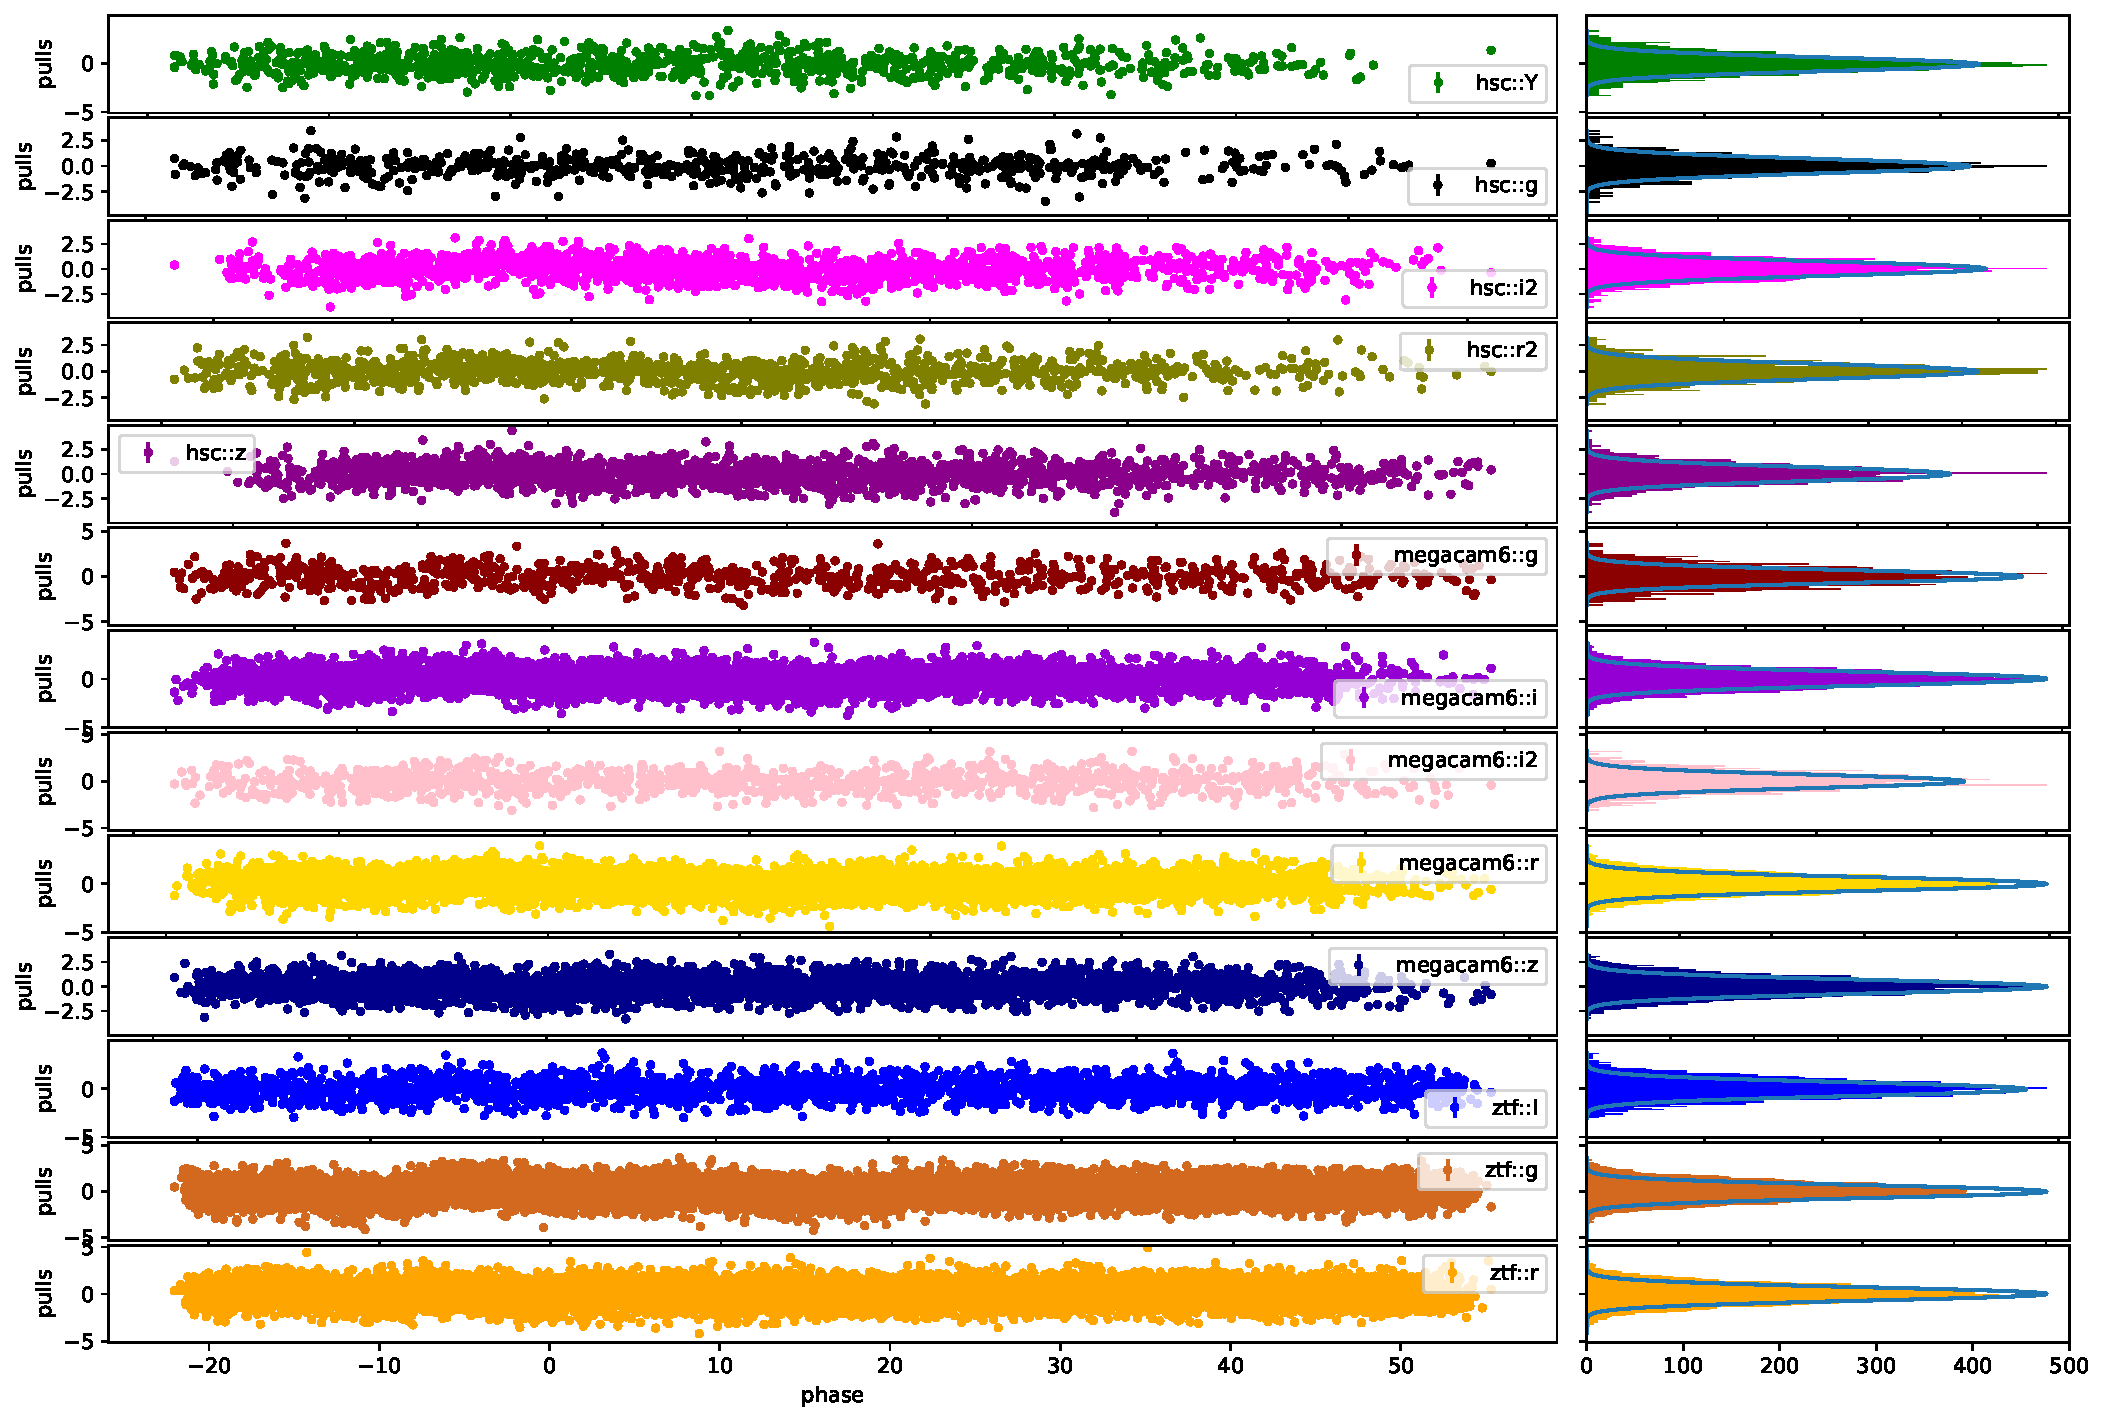
\includegraphics[width=1\textwidth]{MainLayout/DC_chapter/figures/band_resid.pdf}
    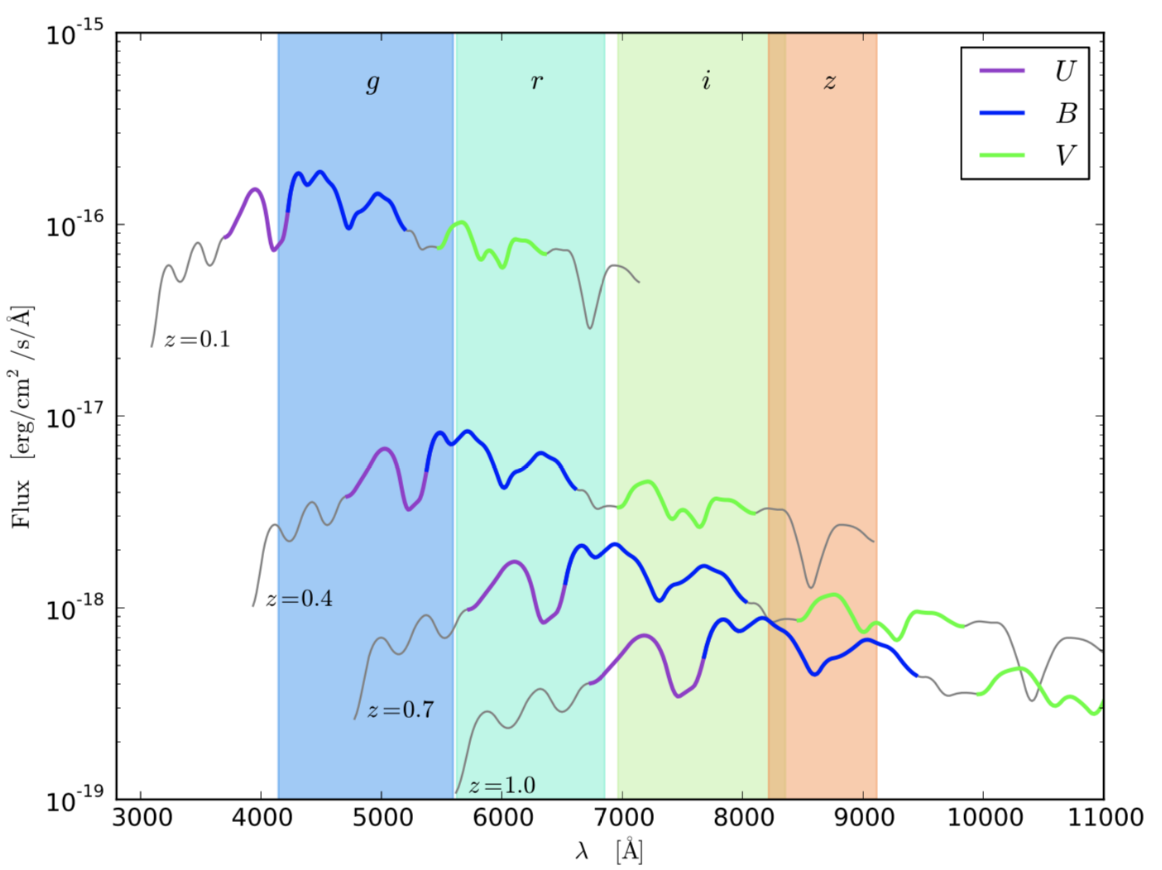
\includegraphics[width=1\textwidth]{MainLayout/NaCl_chapter/figures/flux_evolution.png}
    \caption{Examples of four spectra at different redshifts 0.1, 0.4, 0.7 and 1.0. The highlighted parts of the spectra represent restframe band would measure. The highlighted areas on the graph are the regions where the observer bands measure.}
    \label{fig:flux_evolution}
\end{figure}

The classic approach to convert the observed fluxes and magnitudes into restframe is to apply a K-correction \cite{hogg2002kcorrection}. This allows us to compare observed
fluxes in the same restframe band which is essential to modeling type Ia supernova and measuring the cosmic expansion. The idea is to then describe the supernova magnitude
in the restframe $B^*$ where Type Ia supernovae are standardizable. \\

We define the restframe spectral flux density surface $\mathcal{S}(\lambda, p)$ the spectrophotometric evolution of Type Ia supernova. This will be the quantity that we will
be determining in order to measure the supernovae distances. It's important to note that the spectral flux density $\mathcal{S}$ is determined empirically as the efforts to develop a realistic theoretical 
description of the spectral flux density are extremely difficult (\cite{Blinnikov_2006_difficult_theory}, \cite{R_pke_2018_difficult_theory},  
\cite{Pakmor_2024_difficult_theory}). It's also important to note that we need to use both spectral and photometric data. 
The reason for that is that it is difficult to obtain spectral data over a large phase range and it is to difficult to accurately calibrate the spectra. 
The photometric data then becomes crucial to infer distances while spectra allow us to determine the fine features of the model.\\


\subsection{Models trained on photometric \& spectroscopic datasets}

Here we present some of the empirical spectrophotometric models as well the state of the art SALT models.\\

\noindent \textbf{\underline{MLCS2k2}} \\

The MLCS2k2 model (\textit{Multicolor Light-Curve Shapes 2002}) was 
developed for the analysis of the \textit{High-Z Supernova Search Team} (\cite{Riess_1996}). It describes the observed magnitude of a supernova at a 
specific time phase. The model directly fits a series of functions that describes the lightcurves in a specific band as well as multiple parameters 
including the time of maximum emission of light in the B band restframe $ t_{max}^B$ and an error model. This is the only model I will be
describing here that gets adjusted to describe a function that describes the data. The other models are directly fitted
on the data. It is important to note that there isn't a parameter that describes the supernova color variation since it is assumed 
to be associated with the galactic dust extinction. Before adjusting the 
model parameters, a K-correction is applied to every supernova. \\

\noindent \textbf{\underline{SALT/SALT2/SALT3}} \\

The SALT model (Spectral Adaptative Light curve Template, \cite{Guy_2005}) was developed for the analysis of the SNLS data. The spectral surface $\mathcal{S}(\lambda, p)$
was designed to be capable of varying with 2 parameters that represent the stretch and color of the supernova. This was the first model to include a global parameterization of
supernovae.
The SALT model was pushed further with SALT2 (\cite{Guy_2007_SALT2}) by applyig a Principal Component Analysis (PCA) . This was done by modeling $\mathcal{S}(\lambda, p)$ with two 2-D
surfaces that are described by a base of splines. It's important to note that in SALT2 no K-corrections are applied, instead an offset in the $B^*$ is applied and the measured 
fluxes are brought to restframe. Finally, a later model was publish with the exact same parameterization of SALT2 called SALT3 (\cite{Kenworthy_2021_SALT3}) where the model was
retrained on a larger dataset. \\

\subsection{Models trained on the SNfactory dataset}

SNfactory is a survey that ran from 2004 to 2014 collecting a sequences of spectra of nearby supernovae over a long period of time, thus making the SNfactory dataset (\cite{snfactory}). This is the only dataset that contains a fine spectroscopic description in a large phase range. The well calibrated spectra in the SNfactory dataset will also mean that it doesn't need to be accompanied by photometric measurements to measure distances. \\
These features makes this dataset unique and very interesting to use in order to study the properties of supernova. However it cannot be used alone to measure cosmological parameters such as $w$ since the furthest supernova is at redshift $z\approx0.11$. \


\noindent \textbf{\underline{SNEMO}} \\

SNEMO model (SuperNova Empirical MOdels, \cite{Saunders_2018_SNEMO}) generalises the PCA used in SALT2. In SNEMO, the $\mathcal{S}(\lambda, p)$ components are extracted
using an Expectation Minimization for Factor Analysis or EMFA that takes into account the measurement uncertainties that affects the model. With SNEMO 
multiple model trainings can be done at different orders. At the second order, the $\mathcal{S}(\lambda, p)$ is described with 2 parameters that represent the color and
stretch of the supernova where comparisons with the SALT2 color and stretch parameters have shown strong correlations. \\ 

\noindent \textbf{\underline{SUGAR}} \\

SUGAR (SUpernova Generator And Reconstructor, \cite{L_get_2020_SUGAR}) uses EMFA like SNEMO but applied in a different space with the idea that
supernova variability is encoded in their spectral data. The founders of SUGAR have chosen 13 spectral feautres to identify the supernova variability. The work
with SUGAR has essentially showed that the supernova variability can be captured by 3 parameters, one more than the traditional stretch and color parameters. \\

\noindent \textbf{\underline{Twins Embedding}} \\

The Twins Embedding model (\cite{Boone_2021_twins_embedding}) uses a non-linear parameterization to describe the supernova diversity. It uses a new standardization
method based on the spectral differences between supernova at specific regions. This is also called the spectral distance. If the spectral distance between two supernovae is
small enough they are considered as "Twins". The model is adjusted using an algorithm that does non-linear dimensionality reduction called Isomap which is a generalization of 
PCA while accounting for non-linearities. \\

\noindent \textbf{\underline{SuPAErnova}} \\

The SuPAErnova model (\cite{Stein_2022_PAE}) uses a probabilistic autoencoder in order to assess the supernova diversity. The use of machine learning (ML) in this case 
leaves the model free to explore different ways to determine the necessary parameterization in order to describe the data. The only setback is that it then becomes difficult
to have a physical interpretation of the final parameters. \\
\section{NaCl framework}

The first part of my work for this thesis was the continuation of the development of a new framework designed to train spectrophotmetric models of type Ia supernova called NaCl ("Nouveaux Algorithmes de Courbes de Lumière") which was initially started by G. Augarde during his PhD, defended in September of 2022 (\cite{augar2022}).

In this section we will be defining the model that is trained by NaCl, this includes the parameterization of the model, the model constraints, regularization and error models. Finally we will be detailing how do we practically implement this into a code that can be used.

\subsection{The idea behind the framework}

The framework is meant to be able to easily train a spectrophotometric model all while being able to accurately propagate all know sources of uncertainties. It is meant to be easy to use and manipulate in order to account for any new developments in how spectrophotmetric models are parameterized. The idea is to then have a framework that is fast and capable of conducting model training easily every time one can do so on a cosmological dataset of type Ia supernova. We will see how this will allow us to overcome issues previous spectrophotometric models have encountered, such as calibration issues.

\subsection{Differences with the SALT models}


This parameterization is a classic principal component analysis, or PCA, with the addition of a color law. This presumes that the evolution of a supernova can be known with the help of 2 parameters : the stretch parameter $X_1$ and the excess color parameter $c$. The $M_0$ and $M_1$ surfaces along with the $CL$ color law are common to all supernovae. $M_0$ is the average spectral surface of a type Ia supernova, which represents what your average spectrophotometric evolution of a type Ia supernova looks like.
$M_1$ is a surface representing the main variations to $M_0$. $CL$ represents the color diversity of supernovae. It's also important to note that in NaCl we also determine the date of maximum emission of light $t_{max}$, which is hidden in the model parameters. Finally, in order to take into account the fact that the spectra aren't properly calibrated, we fit a third degree polynomial $SpecRecal(\lambda)$ for each spectra in the training dataset.\\

In practice we will be looking for $X_0$ as well so our spectral flux density will be written as $X_0 \times \mathcal{S}(\lambda,p)$. \\

To summarize, with the SALT2 parameterization, we are looking for global parameters that are $M_0$, $M_1$ and $CL$ common to all supernova and individual parameters $X_0$, $X_1$, $c$ and $t_{max}$ specific to each supernova. Determining the global parameters is what we called "training the model" while determining the individual supernova parameters is called "fitting the lightcurve parameters". In NaCl however, we are performing both at the same time and in this chapter they will be referenced together as "training" the model.


\subsubsection{Practical implementation of the SALT2 model}

In order to be able to determine the global model surfaces ($M_0$ and $M_1$), we will be describing them with the help of B-splines. This is a particular set of polynomials of order $m-1$, called splines of degree $m$, that can form a basis. Their smoothness will allow our model surfaces to have complex forms. We use splines of degree 4 in NaCl. $M_0$ and $M_1$ are then defined as :

\begin{equation}
    M_{0|1}=\sum_{k=1}^{n_p} \sum_{l=1}^{n_{\lambda}} \theta_{kl}^{[0|1]} \mathcal{B}_k(p) \mathcal{B}_l(\lambda)
    \label{eqn:model_spline}
\end{equation}

where $\mathcal{B}$ are the splines, $\theta$ are the model parameters that we will determine.\\

\noindent For the color law $CL(\lambda)$ it is implemented as a degree 5 polynomial. \\

\noindent The model parameters are then determined by minimizing a log-likelihood which takes the form of : 
\begin{equation}
    -2\ln(L) = N\ln(2\pi) + \ln(|\mathbf{V}|) + \mathbf{R}^T\mathbf{V}^{-1}\mathbf{R}
\end{equation}
where $\mathbf{R}$ are the model residuals and $\mathbf{V}$ the covariance matrix independent of the parameters. If $\mathbf{V}$ contains only measurement uncertainties, the problem then becomes minimizing the following quantity : 
\begin{equation}
    \chi^2 = \mathbf{R}^T\mathbf{V}^{-1}\mathbf{R}
\end{equation}
which will be the case for us during this PhD.

\subsection{Constraints}

Since this model is built empirically, we can see that there will be a lot of degeneracies between the individual and model parameters. To break those degeneracies we will be adding a set of constraints.\\ 

When NaCl was first developed, the constraints used were the same as the ones for SALT2 and SALT3 (\cite{Kenworthy_2021_SALT3}) models. 
Although those constraints break the degeneracies that exist between parameters, we've decided to include a new set of constraints that would address two things : the first that one of the constraints is non linear which made the model training take a longer time, the other was that some constraints depended on the supernovae used in the training sample. An example such a constraint was $<X_1> = 0$ which defined the average stretch of a supernovae. This is isn't an issue if we are comparing the stretch of supernovae that were fitted using the same model. However since NaCl will be used to train different models on different datasets, it'll be more difficult to directly compare the parameters of the supernovae.\\

During this PhD, the following sets of constraints were developed. I will be detailing what they do and why they were developed.\\

\noindent \textbf{\underline{\large{Model normalization:}}} \\


The model normalization is degenerated with the value of $X_0$. We impose that : 

\begin{align}
    \int M_0(\lambda,p=0)\frac{\lambda}{hc}B(\lambda)\mathrm{d}\lambda = 1 \label{eqn:M0norm}\\
    \int M_1(\lambda,p=0)\frac{\lambda}{hc}B(\lambda)\mathrm{d}\lambda = 0
\end{align}
where $B(\lambda)$ is the restframe standard $B$-band.\\


\noindent \textbf{\underline{\large{Date of maximum emission:}}} \\

There exists a degeneracy between the model and the date of maximum emission $t_{max}$. It’s possible to
shift the entire model in order to compensate for a change in the date $t_{max}$. For that we impose that at
$p = 0$, the model presents a maxima in the standard $B$-band :

\begin{align}
    \frac{\mathrm{d}}{\mathrm{d}p} \int M_0(\lambda,p=0)\frac{\lambda}{hc}B(\lambda)\mathrm{d}\lambda \Big{|}_{p=0} = 0 \\
    \frac{\mathrm{d}}{\mathrm{d}p} \int M_1(\lambda,p=0)\frac{\lambda}{hc}B(\lambda)\mathrm{d}\lambda \Big{|}_{p=0} = 0
\end{align}
\\

\noindent \textbf{\underline{\large{Color Law:}}} \\

We also need to account for the degeneracy that exists between the spectral shape of the model and $CL$. Tilting the $M_0$ and $M_1$ can be completely corrected for by changing $CL$. We impose then that $CL(B) = 0$ and $CL(V ) = 1$ with $B$ and $V$ being the central wavelengths of the restframe standard $B$-band and $V$-band.\\


\noindent \textbf{\underline{\large{Average color:}}} \\

Another degeneracy exists between the individual supernova color $c$ and the $M_0$. Changing the spectral features of the model can be completely compensated by the value of $c$. For that we need to define the "average" supernova color. 
We impose that the the $M_0$ surface would have its $B - V$ color equal to 0 at peak luminosity and that $c$ accounts for the relative variations in color with respect to that. The constraint now becomes :

\begin{equation}
    \int \left[ M_0(\lambda, p=0)B(\lambda) - M_0(\lambda, p=0)V(\lambda)   \right] \frac{\lambda}{hc} \mathrm{d}\lambda = 0
\end{equation}\\

\noindent \textbf{\underline{\large{Average stretch:}}} \\

A similar degeneracy also exists with $X_1$. A global change of the $X_1$’s can be absorbed by changing the shape of the $M_0$ surface along the phase axis. We have decided to fix the value of $X_1=1$ such that it would be equivalent to having the same $X_1$ value using SALT2. For that we fix the difference between the model evaluated for $X_1=0$ and $X_1 = 1$ at a phase of 15 :

\begin{equation}
    \int \left[M_0(\lambda, p=15) + M_1(\lambda, p=15) \right] \frac{\lambda}{hc}B(\lambda) \mathrm{d}\lambda - \alpha \int M_0(\lambda, p=15) \frac{\lambda}{hc}B(\lambda) \mathrm{d}\lambda = 0
\end{equation}
with $\alpha = 10^{-0.4 \times 0.162}$ the flux difference we have found in SALT2. \\

\noindent \textbf{\underline{\large{Average width:}}} \\

The last unwanted degree of freedom is regarding the width of the model. We can see that the definition of $X_1$ relies on a difference between the model with different stretch parameters but it doesn’t define what the width of the model is. We can always make the model larger or smaller while maintaining the constraints on all of the other parameters. One way to bypass that issue is to constrain the model at a certain phase. We choose to fix the model at a phase $p=15$, also known as $\Delta m_{15}$ as : 

\begin{equation}
    \int M_0(\lambda, p=15) \frac{\lambda}{hc} \mathrm{d}\lambda = 10^{-0.4}
\end{equation} \\

In practice, we write down the constraints as a function $C_k(\beta) = \alpha_k $ where $C_k(\beta)$ is a function evaluating the $k$-th constraint of value $\alpha_k$. This is then added as penalty that takes the form $\mu_{cons}\sum_k (C_k(\beta)-\alpha_k)^2$ where $\mu_{cons}$ is hyperparameter that determines the strength of the penalty. We can write this in a matrix $\mathbf{C}(\beta)$ and we obtain :

\begin{equation}
    \boxed{\chi_{cons}^2 = \mu_{cons} \mathbf{C}(\beta)^T \mathbf{C}(\beta)}
\end{equation}

\subsection{Regularization}

Because our training dataset contains a finite number of data points, it’s impossible that the entirety of the global parameters would be constrained by data. To deal with that we add regularization to the model during the fit, which is a penalty added to the model in the areas where we would have extremely large variations due to poor constraining power of the data. This is specifically really important for NaCl since we are fitting the date of maximum emission there are data points that could go outside of the model range. \\

The regularization penalty that was initially developed was expressed as :

\begin{equation}
    \mu_{reg} \sum_{kl} \left(  \theta_{k,l}^2 + \left( \theta_{k+1,l} - \theta_{k,l} \right)^2   \right)
    \label{eqn:old_reg}
\end{equation}

 where $\theta_{kl}$ are the model parameters as seen in equation \ref{eqn:model_spline}. The first sum is a penalty that makes the $\theta$'s tend to zero when no data is available. The second term is a penalty of the phase derivatives of the surfaces that limits the sharp variations of the model observed when no data is available, or at poorly constrained regions of the model. Finally, $\mu_{reg}$ is a hyperparameter that determines the strength of the penalty. Writing this in a matrix form gives us :

 \begin{equation}
     \chi^2_{reg} = \mu_{reg}\beta^T \mathbf{P} \beta
     \label{eqn:chi2_reg_old}
 \end{equation}
 where $\mathbf{P}$ is what we call the regularization matrix, that allows us to obtain the expression in equation \ref{eqn:old_reg}, and $\beta$ our set of parameters. \\
 An issue that we've had with this form of regularization is that it is very sensitive to the value of $\mu_{reg}$. If it's too small the model continues to present very strong variations. If it's too strong the model becomes attenuated and this biases our parameters, which means the cosmological parameters calculated with the output of NaCl would be biased. We show the effects of the strength of the regularization on the model in Figure \ref{fig:regularization} \\ 


 \begin{figure}[htpb]
\centering
\begin{subfigure}{0.9\textwidth}
    \centering
    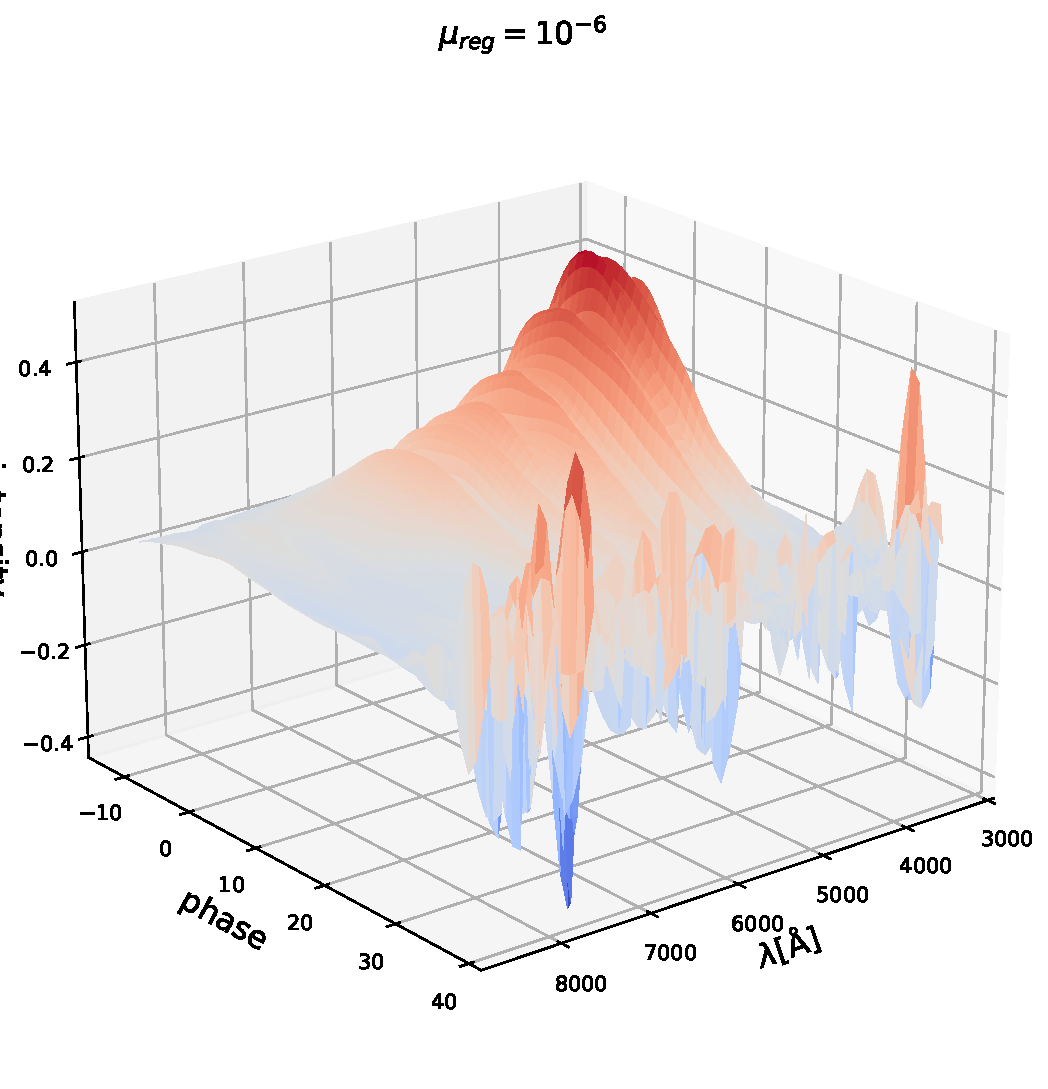
\includegraphics[width=.7\textwidth]{MainLayout/NaCl_chapter/figures/m0_e6_reg.pdf}
    \caption{}
    \label{fig:weak_reg}
\end{subfigure}%

\vspace{1em}

\begin{subfigure}{0.9\textwidth}
    \centering
    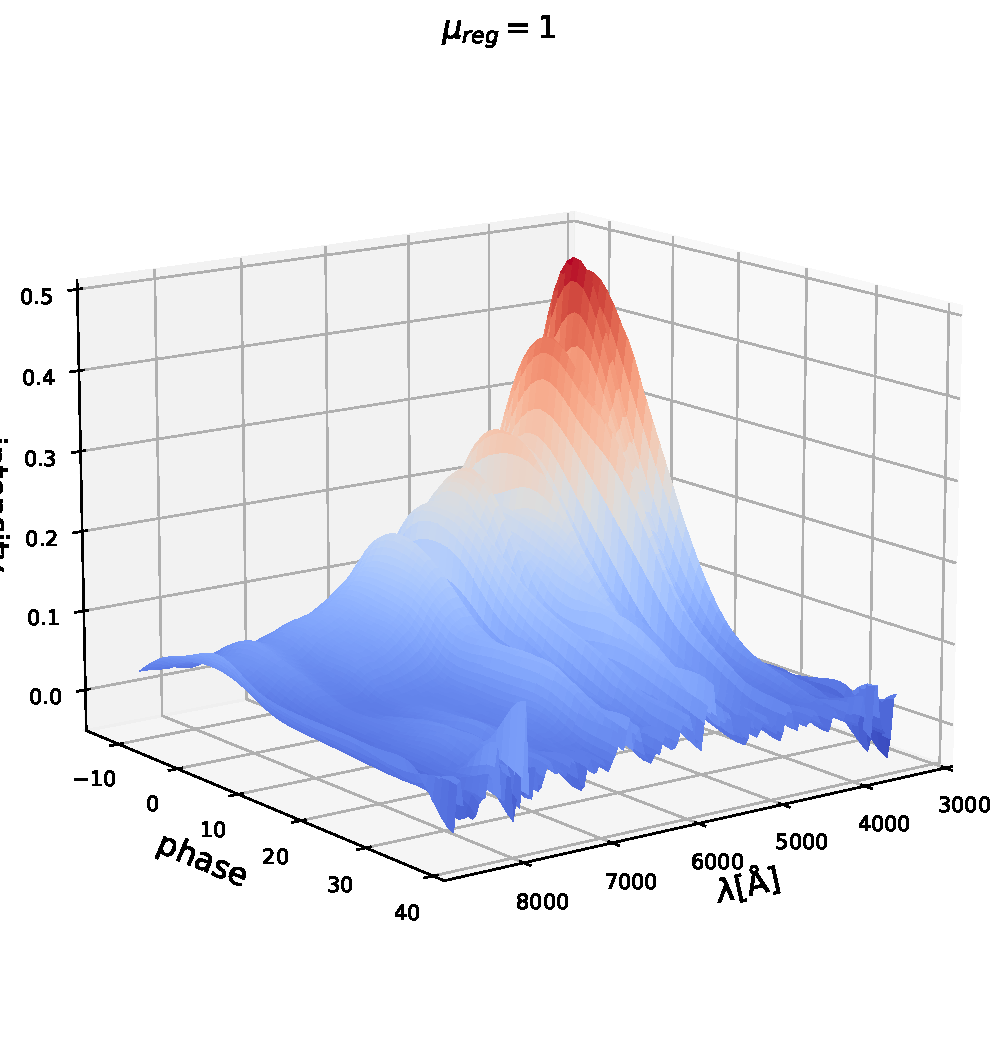
\includegraphics[width=.7\textwidth]{MainLayout/NaCl_chapter/figures/m0_e0_reg.pdf}
    \caption{}
    \label{fig:strong_reg}
\end{subfigure}
\caption{Effects of the strength of the regularization on the shape of the $M_0$. In \ref{fig:weak_reg} we see how the model behaves with a $\mu_{reg}=10^{-6}$. In \ref{fig:strong_reg} we see how the model behaves with a $\mu_{reg}=1$.}
\label{fig:regularization}
\end{figure}

To try and overcome this issue, I've developed during this PhD a regularization scheme that adapts the force of the regularization based on the number of points seen by each model parameter. This regularization scheme is inspired by \cite{lenz2022adaptiveregularizationbsplinemodels}. We can separate $\mathbf{P}$ matrix as follows : 

\begin{equation}
    \mathbf{P} = \mathbf{P}^{data} + \mathbf{P}^{smooth}
\end{equation}

with $\mathbf{P}^{data}$ and $\mathbf{P}^{smooth}$ the matrices determining the strength based on the number of points and to smoothen the model where there is no data as much as possible. In order to determine $\mathbf{P}^{data}$, we define $\mathcal{N}_i$ as the number of data points seen by each $\theta_{i}$ parameters ($\theta_{kl}$ written as a vector). We then introduce for each $\mathcal{N}_i$ a parameter $\mu_i$ which will act as a gate function of $\mathcal{N}_i$. This will determine the force of our regularization. The idea is that if $\mathcal{N}_i=0$ we regularize model strongly, otherwise we don't.\\

\textcolor{red}{COMMENT : This specific version of the regularization wasn't implemented in the final version of NaCl since we still had to test other things in between. I will be rewriting this part of the manuscript again.}

$\mu_i$ is then defined as : 

\begin{equation}
  \mu_i^{data} = \mathrm{max}(\mu_{reg}^{data} - \mathcal{N}_i, 0)
  \label{eqn:reg_mu}
\end{equation}

We can use that to define a diagonal matrix $\mathbf{M}^{data}$ where $\mathbf{M}_{ii}^{data} = \mu_i^{data}$. It is then clear that the simplest way to define $\mathbf{P}^{data}$ will be to write it as :

\begin{equation}
    \mathbf{P}^{data} = \mathbf{M}^{data} \times \mathbb{1}
\end{equation}

\noindent We then define $\mathbf{P}^{smooth}$ as a penalty on the first order derivative of the model in phase, like in equation \ref{eqn:old_reg}. We apply the same adaptive method mentioned previously and we get :

\begin{equation}
    \mathbf{P}^{smooth} = \mathbf{M}^{smooth} \times \mathbb{P}
\end{equation}

with $\mathbb{P}$ being : 
\begin{equation}
     \mathbb{P} = \begin{bmatrix} 
     2  & -1& 0  &   &     &...  \\
     -1 & 1 & -1 & 0 & ... & \\  
     0  &   &    &...&     &  \\  
        &   &... &   &     &  0\\ 
        &...& 0  & -1& 1   & -1 \\  
     ...&   &    & 0 & -1  & 2 \end{bmatrix}
\end{equation}
with $\mu_{reg}^{smooth}$ would be the hyperparameter determining the strength of the regularization on the derivatives.\\
Since the hyperparameters are now included in the  $\mathbf{P}$ matrix, the penalty now becomes : 
\begin{equation}
     \boxed{\chi^2_{reg} = \beta^T \mathbf{P} \beta}
     \label{eqn:chi2_reg_new}
 \end{equation}

\subsection{Error models}

Dealing with an empirical model means that we expect that our model would not perfectly describe the data. More specifically, the residuals of the model would not be explained solely by the measurement uncertainties on the data. This is a variability that exists between supernovae, unable to be captured by the SALT2 parameterization.\\
It's also important to note that all of the photometric measurements are affected by uncertainties of the photometric instruments. This can play a crucial role in our measurements of cosmological parameters as it has been shown in the most recent analyses to be one of the leading systematics (\cite{rubin2024unionunitycosmology2000}, \cite{vincenzi2024darkenergysurveysupernova}).\\
We can account for both the supernova variability and calibration uncertainties with the help of error models.\\

\subsubsection{Error Snake}

The first error model is the Error Snake, which is supposed to capture errors directly due to variability in the flux. If we call $V$ the variance of the data points, then the error model is implemented as :
\begin{equation}
    V = \sigma_{meas}^2 + \sigma_{snake}^2
\end{equation}
where $\sigma_{meas}$ are the measurement uncertainties and $ \sigma_{snake}$ is the additional variance added that is our Error snake model.\\

The general expression of this term is :
\begin{equation}
    \sigma_{snake} = G(\lambda, p) \times \phi(\lambda,p)
\end{equation}
where $\phi$ is the concatenation of both the measured photometric and spectroscopic fluxes used in our training dataset. $G(\lambda, p)$ can take multiple forms depending on how we would like to model our Error snake. \\

The simplest way to model it would be as a constant. The expression becomes : 
\begin{equation}
    G(\lambda, p) = g
\end{equation}
Physically this means that the variability of the supernovae in our dataset are independent of phase and wavelength.\\

Alternatively, we can imagine something more complex by modeling $G$ as a surface like $M_0$ and $M_1$ that is to be determined during the training. The expression then becomes:
\begin{equation}
    G(\lambda, p) = g(\lambda, p)
\end{equation}
Here, the variability does depend on phase and wavelength.\\

Lastly, we thought of adding a bit more complexity in our Error snake since we know that it's possible that our dataset could be contaminated by very peculiar supernovae or by objects that are hard to distinguish from type Ia supernova such as type Ib and type Ic supernovae or . We decided to also include an extra term in $G$ that takes up one value for each supernova in our dataset, we call it $\gamma_{SN}$. We expect that the $\gamma_{SN}$ value of a peculiar supernova would be larger than the others. The expression then becomes : 

\begin{equation}
    G(\lambda, p) = \gamma_{SN} \times g(\lambda, p)
\end{equation}

which is what we would like to use in the final analysis of the LEMAÎTRE dataset. However it is important to note that for the data challenges, specifically DC1 (see Chapter 4), we will be using the simplest form of the Error snake.

\begin{figure}[htpb]
\centering
\begin{subfigure}{1\textwidth}
    \centering
    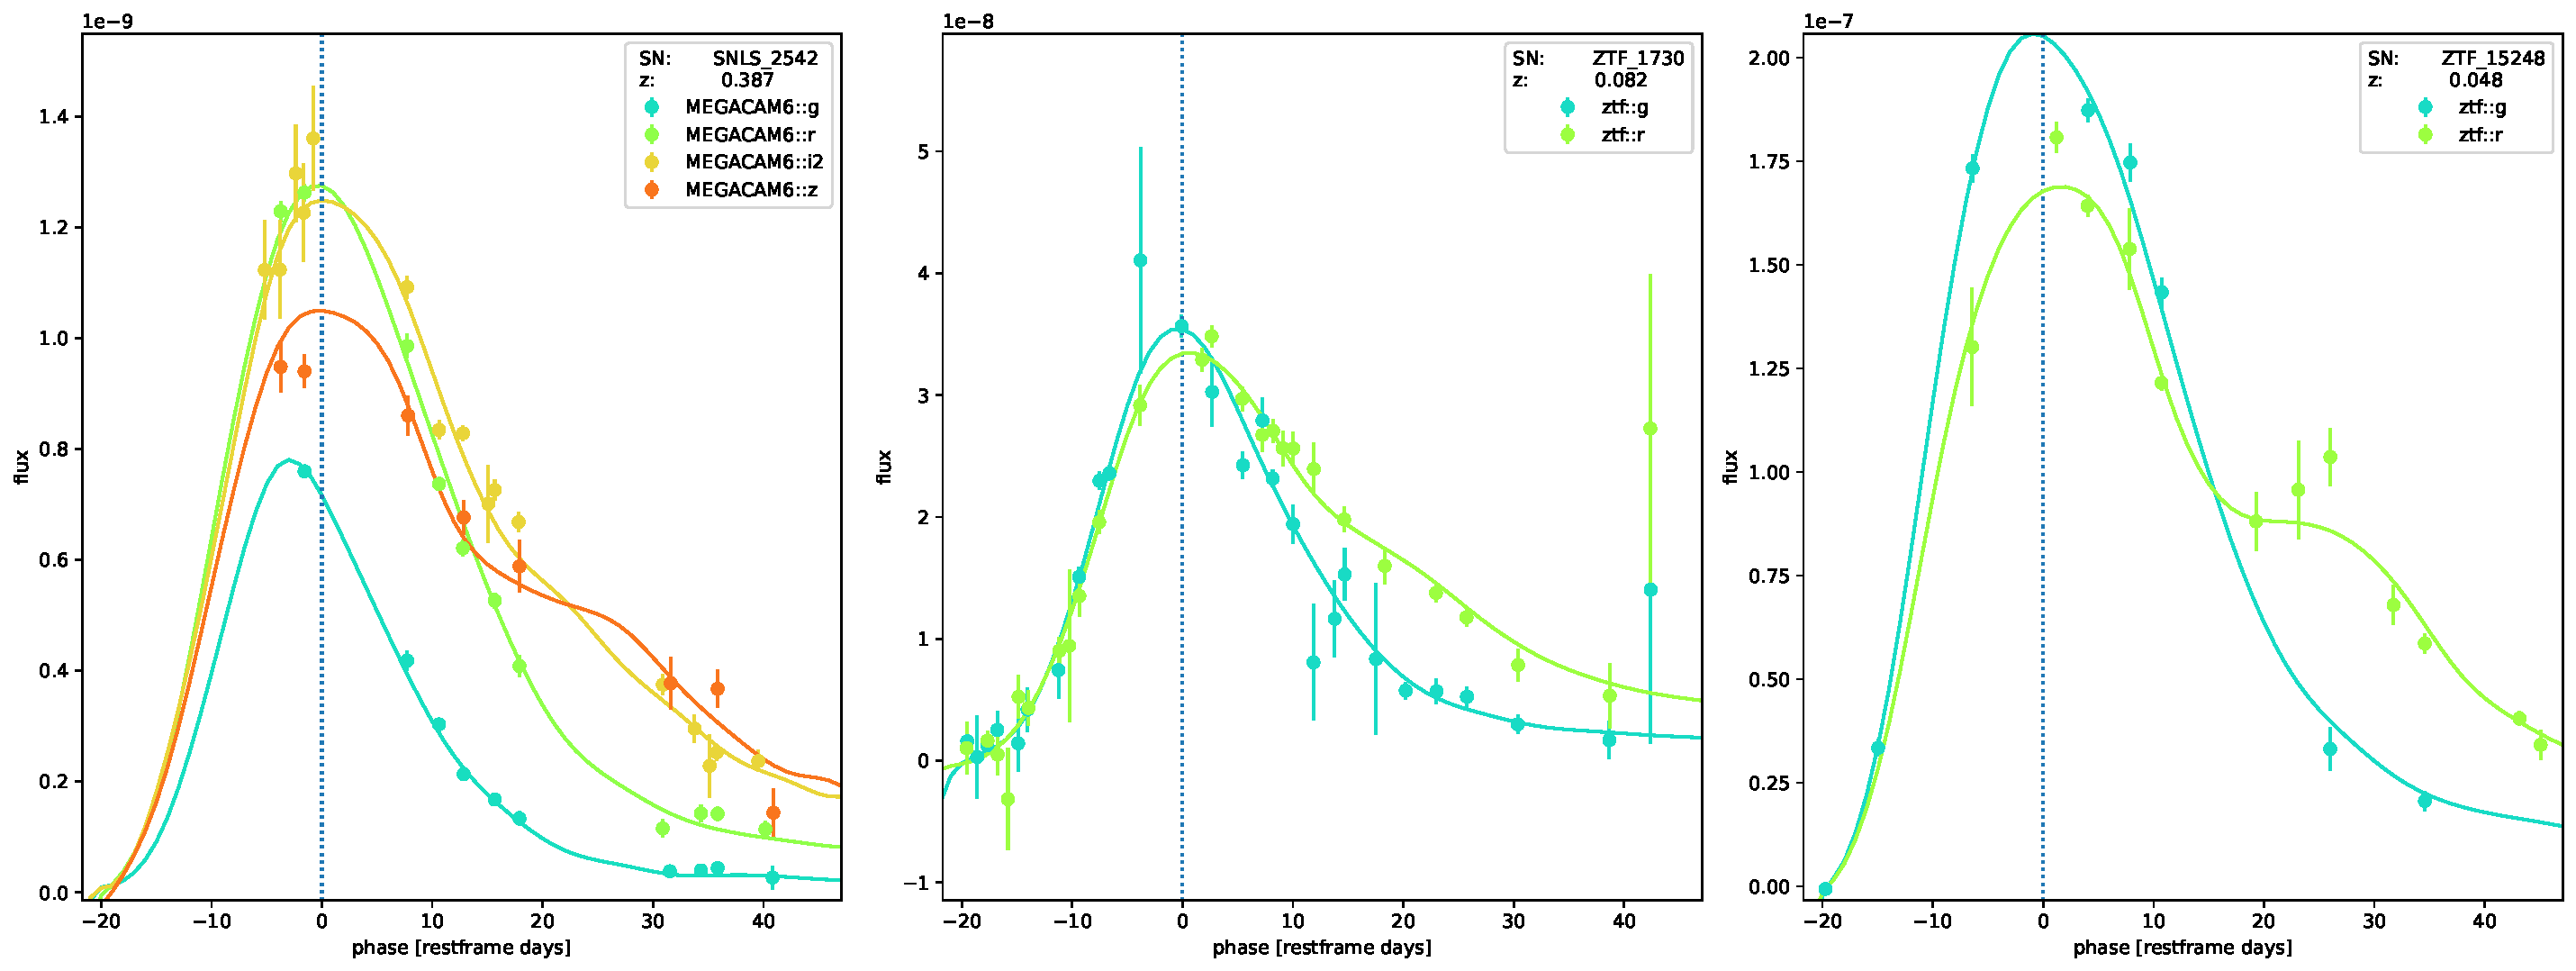
\includegraphics[width=1.1\textwidth]{MainLayout/NaCl_chapter/figures/lcs_without_snake.pdf}
    \caption{}
    \label{fig:nosnake}
\end{subfigure}%

\vspace{1em}

\begin{subfigure}{1\textwidth}
    \centering
    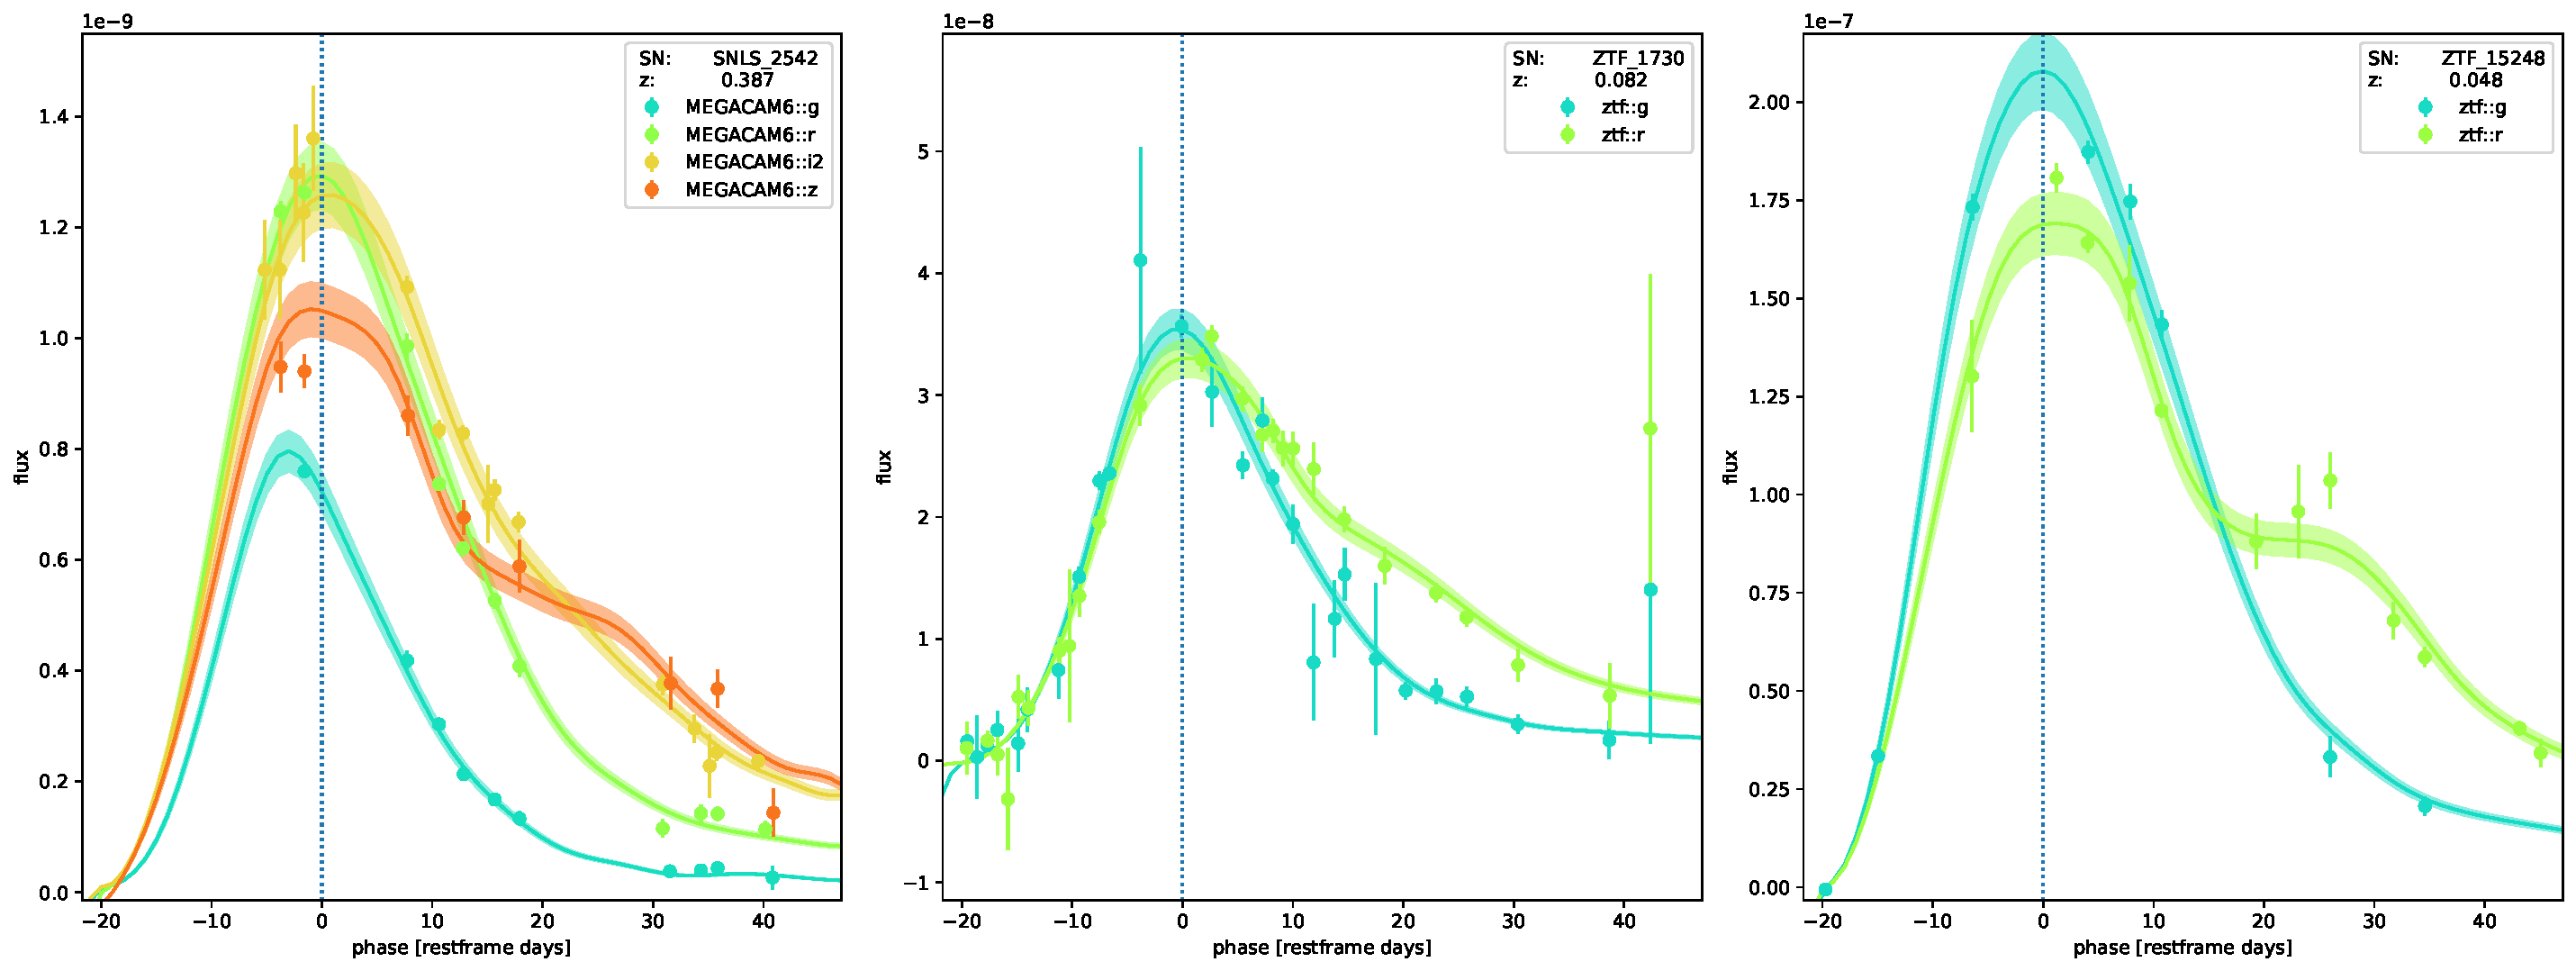
\includegraphics[width=1.1\textwidth]{MainLayout/NaCl_chapter/figures/lcs_with_snake.pdf}
    \caption{}
    \label{fig:snake}
\end{subfigure}
\caption{Visual representation of the error snake on simulated lightcurves from DC1 (see section (reference)). In \ref{fig:nosnake} we see how the model represents the data without an error snake model. In \ref{fig:snake} we see a highlighted section for each lightcurves which are the variations modeled by the error snake.}
\label{fig:errorsnake}
\end{figure}

\subsubsection{Color Scatter}

\noindent \textcolor{red}{COMMENT : Waiting for the final implementation}

\subsubsection{Calibration Uncertainties}

The calibration uncertainties are taken into account directly in the model. One parameter $\eta$ is added for each transmission band in our dataset held by a prior that is known beforehand. For the LEMAÎTRE project we have 12 bands, so we'll have 12 $\eta$ parameters. The expression of the photometric model becomes : 

\begin{equation}
    \phi_{phot}(\lambda, p) = X_0 (1+\eta) (1+z) \int S(\lambda, p) T(\lambda) \frac{\lambda}{hc}\mathrm{d}\lambda
\end{equation}

With an additional penalty to the model :

\begin{equation}
    \chi^2_{calib} = \mathbf{\eta}^T \mathbf{V_{\eta}}^{-1}\eta
\end{equation}
$\mathbf{V_{\eta}}$ being the $\eta$ covariance matrix that is already known.


\subsection{NaCl output}

At the end of a training, we get a vector containing all of the model and individual supernova parameters and the full covariance
 matrix calculated from the Hessian of the model : $  \mathbf{V} = 2 \mathbf{H}^{-1}$. For the cosmological analysis, we will be marginalizing 
 over all but the $X_0$, $X_1$ and $c$ parameters. \\

\begin{figure}[ht]
    \centering
    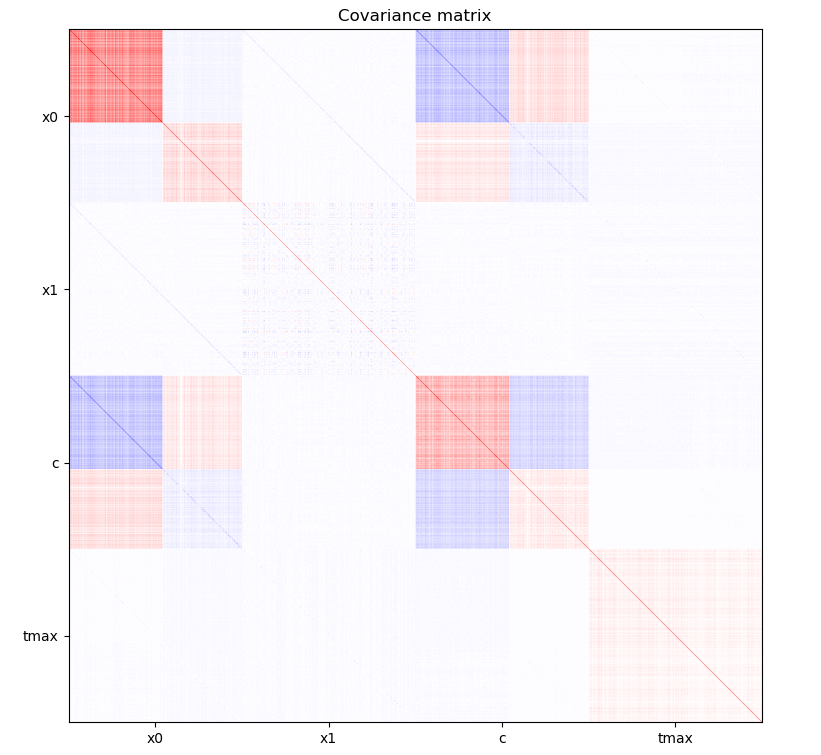
\includegraphics[width=1.0\textwidth]{MainLayout/NaCl_chapter/figures/covariance matrix.png}
    \caption{Example of the NaCl covariance matrix after an output, marginalized over all but the $X_0$, $X_1$ and $c$ parameters.}
    \label{fig:corr_mat_nacl}
\end{figure}
\section{NaCl on real data} \label{sec:nacl_real_data}

There have been models that were empirically constructed in similar ways as the SALT models with SNfactory data, namely SNEMO (\cite{Saunders_2018_SNEMO}), 
SUGAR (\cite{L_get_2020_SUGAR}), Twins Embedding (\cite{Boone_2021_twins_embedding}) and SuPAErnova (\cite{Stein_2022_PAE}) as presented earlier. 
These models usually incorporate different parameterizations than SALT2 in order to try and fully understand the spectrophotometric evolution of supernovae. 
One thing to note is that it is easy to implement different models in NaCl. So one could modify the current implementation of the SALT2 model and add 
extra parameters and test if it improves the description of supernovae. \\
For now, we present the results obtained when training NaCl on the SNfactory data with a SALT2 parameterization. \\

\subsection{NaCl training results}
\subsubsection{Data coverage}

Training a SALT2-like model with NaCl on the SNfactory was the first time NaCl was used on real data and was part of the PhD to test the framework. 
The SNfactory dataset used here contains 224 supernova and 3135 spectra. We can see in the coverage of the data on the model's $\lambda-p$ space in 
Figure \ref{fig:snf_coverage} that we have a very rich dataset that covers a very large part of the model's domain of definition. 

\begin{figure}[ht]
    \centering
    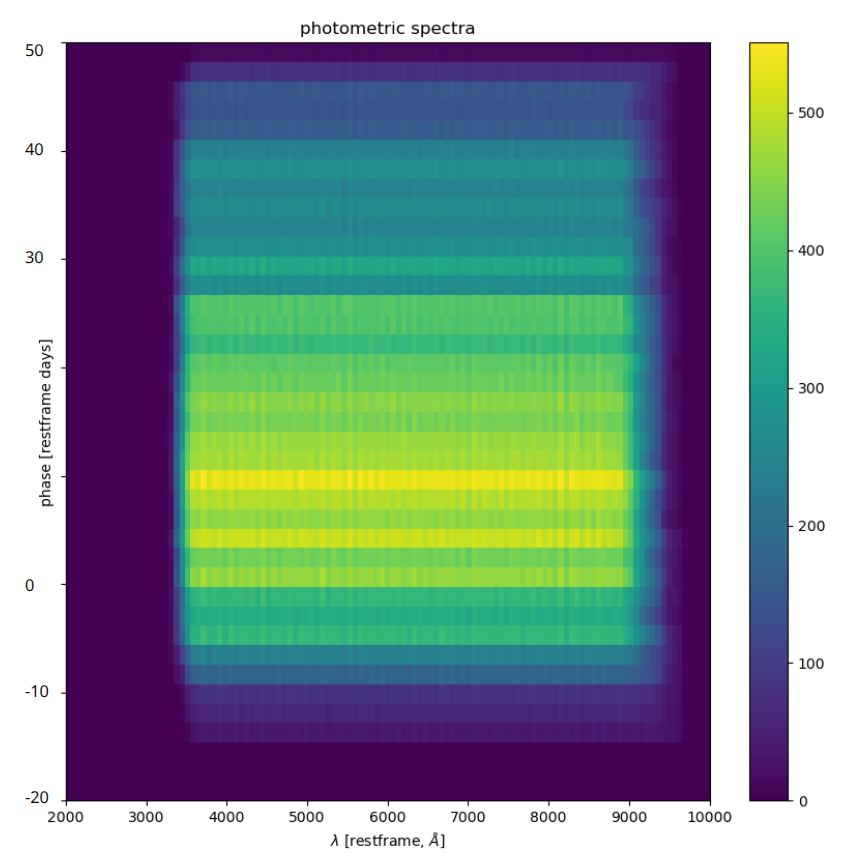
\includegraphics[width=0.7\textwidth]{MainLayout/NaCl_chapter/figures/snfactory/coverage.png}
    \caption{Coverage of the SNfactory data in the $\lambda-p$ space.}
    \label{fig:snf_coverage}
\end{figure}

\subsubsection{Fitting the spectra}

We present in Figure \ref{fig:snf_spectra} examples of spectra that were fitted with NaCl. These are 2 spectra randomly picked out that belong to two different supernova 
and are taken at different phases. What we see is that the trained model seems to accurately describe the evolution of those spectra. The errorsnake model employed 
shows an intrinsic dispersion of the fluxes at an order of about 10\%. We present in the next subsection the results of full dataset.\\

 The entirety of the model training takes around 30 minutes on a Dell Precision 3581 laptop 
equipped with an Intel(R) Core(TM) i7-13700H, 14 cores, up to 5.0 GHz, 32 GB RAM and a NVIDIA RTX A1000 6GB GPU. \\

\begin{figure}[htpb]
\centering
\begin{subfigure}{0.9\textwidth}
    \centering
    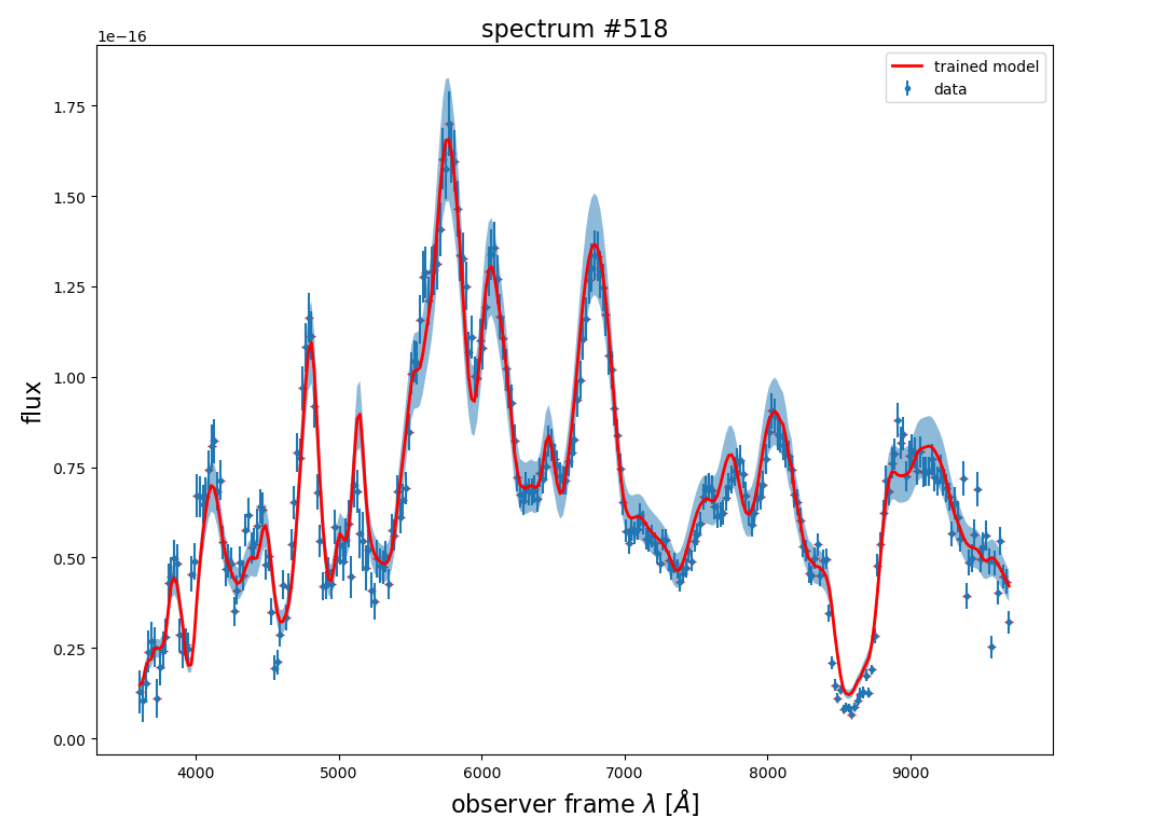
\includegraphics[width=0.9\textwidth]{MainLayout/NaCl_chapter/figures/snfactory/spec_518.png}
    \caption{}
    \label{fig:snf_spec_1}
\end{subfigure}%

\vspace{1em}

\begin{subfigure}{0.9\textwidth}
    \centering
    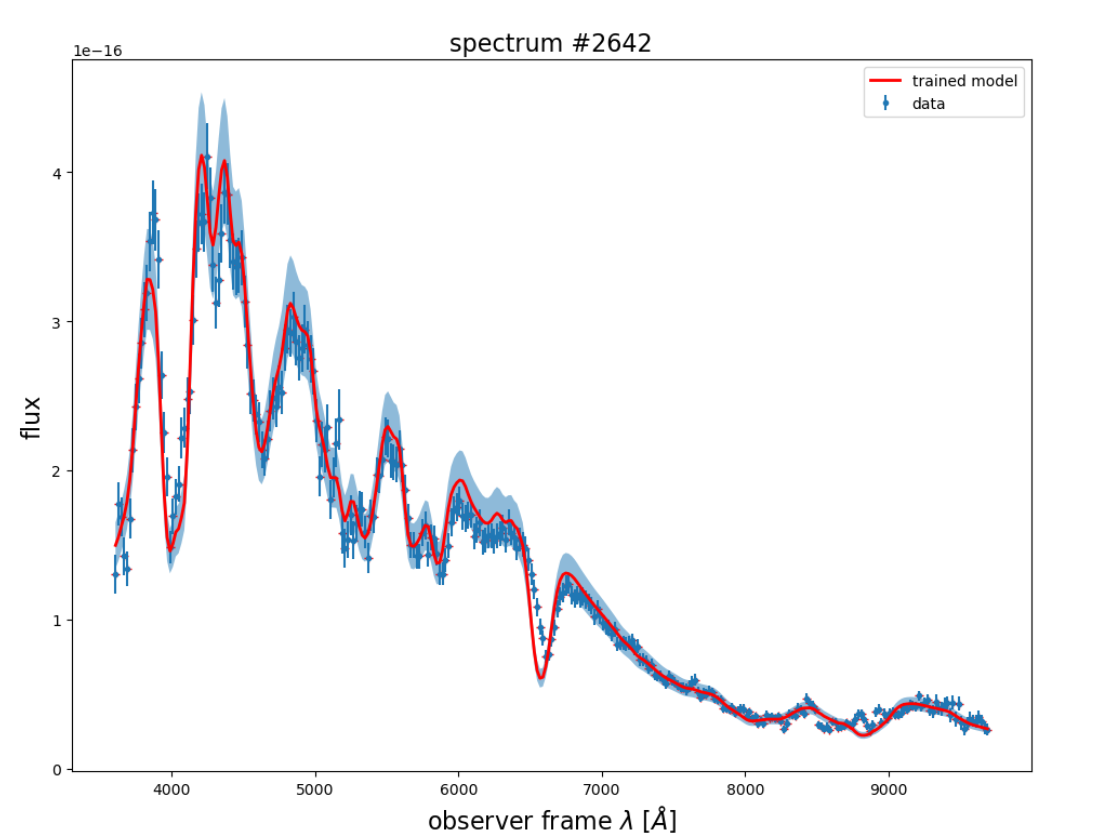
\includegraphics[width=0.9\textwidth]{MainLayout/NaCl_chapter/figures/snfactory/spec_2642.png}
    \caption{}
    \label{fig:snf_spec_2}
\end{subfigure}
\caption{Two spectra with the train NaCl model. The blue points are the data, the red line is the trained model and the highlighted area is the error model.}
\label{fig:snf_spectra}
\end{figure}

\subsubsection{Training residuals}

We would like to examine how well a SALT2 like parameterized model is able to describe the spectrophotometric evolution of supernovae. 
In order to do that, we will be looking at the weighted residuals of the model on the entirety of the data and check if there are any particular features that stand out. 
This is presented in Figure \ref{fig:snf_pulls} where we have calculated the weighted residuals which represent by how many $\sigma$ our model differs from the data, 
also known as pulls. We do that for each data point and stack them on top of each other if they have been observed at the same time. So for example if we have 2 spectra 
measured at phase of $p= -1$ with data points at $5000{\AA}$, it'll appear as one point on the Figure and its value will be the average of the 2 pulls. We then get a 
Figure that represents the accuracy of the model in the $\lambda-p$ space. This also means that each horizontal line represents on average how well a spectrum is modeled 
at that particular restframe phases, while the vertical lines are for specific restframe wavelengths. \\

\noindent We see in the Figure \ref{fig:snf_pulls} that for most of the $\lambda-p$ space the residuals show good agreement between the model and the data. 
But what also stands out is that we can identify three distinct wavelength regions where the model is unable to capture the variability of the data. 
These three regions are found at $\sim 3500 {\AA}$, $\sim 6000 {\AA}$ and $\sim 8000 {\AA}$, which correspond to UV, Si II and Ca II. These are known to 
have very diverse forms (\cite{Wang_2012_UV}, \cite{Parrent_2016_Si_II}) and we can see here that they are not captured by a SALT2 parameterization. 
It is important to mention that the models mentioned in Chapter 2 that go beyond the SALT2 parameterization can capture those variabilities with the help of extra parameters.

\begin{figure}[ht]
    \centering
    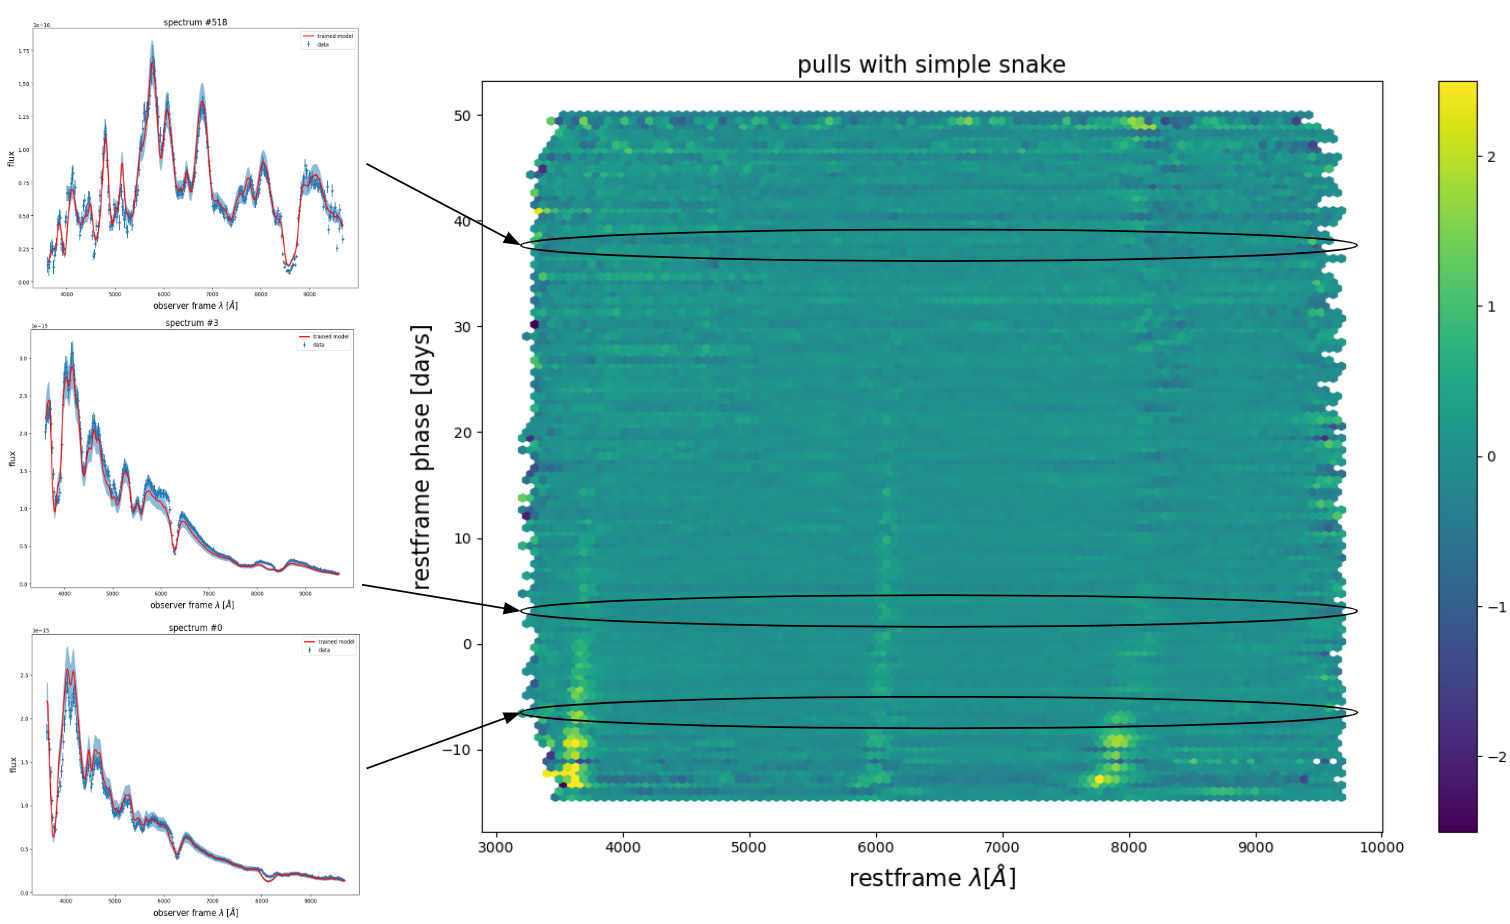
\includegraphics[width=1\textwidth]{MainLayout/NaCl_chapter/figures/snfactory/pulls.png}
    \caption{Weighted residuals at the end of the training done with NaCl on the SNfactory data. The color bar represents by how many $\sigma$ our model differs from the data. We also use as examples 3 spectra at 3 different phases and show where they would be present on the plot.}
    \label{fig:snf_pulls}
\end{figure}


\section{A Training Recipe for NaCl}

The application of NaCl to the \textsc{Lemaître} dataset presents a 
different challenge from the training on SNfactory data. The \textsc{Lemaître} 
sample contains a large number of supernovae and a correspondingly large 
number of model parameters. In this setting, fitting all 
parameters simultaneously from arbitrary initial values can lead to an 
inefficient training procedure. 

In particular, we found that when the initial model parameters are far from 
their optimal values, the error model can absorb part of the discrepancies 
between the model and the data. Although this provides a valid direction for 
the minimizer and can lead to a decrease in $Q(\boldsymbol{\beta})$, it can prevent the 
physical model parameters from being properly constrained during the initial 
stages of the fit. The non-linear nature of the model can also lead the 
minimizer towards undesirable local minima depending on the initial 
parameters. \\

To address these issues, I developed a sequential training procedure that 
provides increasingly informed initial estimates for the different components 
of the model before performing the full fit. This approach reduces the 
sensitivity of the minimization to the initial conditions, improves the 
stability of the training, and reduces the computational cost of the full 
optimization. The resulting training recipe is divided into five steps: 

\begin{enumerate}
    \item \underline{Light curve fit with the initial NaCl model:} 
    Only $X_0$, $X_1$, $c$, and $t_{max}$ are fitted for each 
    supernova, while the global model parameters are kept fixed.

    \item \underline{$SpecRecal$ fit with the initial NaCl model:} 
    The coefficients describing the spectroscopic recalibration are 
    estimated for each spectrum. Since the recalibration model is linear 
    in these coefficients, this step is computationally inexpensive. During this step, all other parameters are fixed at the best value found in the previous step. 

    \item \underline{Initial model guess:} 
    The parameters describing the model surfaces $M_0$, $M_1$, and $CL$ are 
    fitted alongside $X_0$, $X_1$, $c$, $t_{max}$ and $SpecRecal$ with a fixed error model. 
    This is done to obtain an initial model that is sufficiently close to the 
    solution and satisfies the required model constraints.

    \item \underline{Initial error model guess:} 
    With the spectrophotometric model fixed, the parameters of the error 
    model are fitted while the all of the other parameters are fixed to the value found in the previous step. 
    This is done to provide an initial estimate of the error model.

    \item \underline{Full training:} 
    All model, error model, and supernova parameters are released and 
    simultaneously fitted.
\end{enumerate}

The first two steps are computationally inexpensive. The initial model fit 
in step 3 is more demanding because of the large number of parameters 
associated with the $M_0$ and $M_1$ surfaces. Since the purpose of this step 
is only to obtain a suitable starting point for the subsequent optimization, 
the number of minimization iterations is limited to 15. The error-model fit 
in step 4 is again relatively inexpensive. The final step, in which all 
parameters are simultaneously released, constitutes the most computationally 
expensive part of the training.

%\subsection{Regularization}

%To try and overcome this issue, I've developed during this PhD a regularization scheme that adapts the force of the regularization based on the number of 
%points seen by each model parameter. This regularization scheme is inspired by \cite{lenz2022adaptiveregularizationbsplinemodels}. We can separate $\mathbf{P}$ matrix as 
%follows: 

%\begin{equation}
%   \mathbf{P} = \mathbf{P}^{data} + \mathbf{P}^{smooth}
%\end{equation}

%with $\mathbf{P}^{data}$ and $\mathbf{P}^{smooth}$ the matrices determining the strength based on the number of points and to smoothen the model where there is no data as 
%much as possible. In order to determine $\mathbf{P}^{data}$, we define $\mathcal{N}_i$ as the number of data points seen by each $\theta_{i}$ parameters ($\theta_{kl}$ written 
%as a vector). We then introduce for each $\mathcal{N}_i$ a parameter $\mu_i$ which will act as a gate function of $\mathcal{N}_i$. This will determine the force of our 
%regularization. The idea is that if $\mathcal{N}_i=0$ we regularize model strongly, otherwise we don't.\\

%$\mu_i$ is then defined as: 

%\begin{equation}
% \mu_i^{data} = \mathrm{max}(\mu_{reg}^{data} - \mathcal{N}_i, 0)
% \label{eqn:reg_mu}
%\end{equation}

%We can use that to define a diagonal matrix $\mathbf{M}^{data}$ where $\mathbf{M}_{ii}^{data} = \mu_i^{data}$. It is then clear that the simplest way to define 
%$\mathbf{P}^{data}$ will be to write it as:

%\begin{equation}
%   \mathbf{P}^{data} = \mathbf{M}^{data} \times \mathbb{1}
%\end{equation}

%\noindent We then define $\mathbf{P}^{smooth}$ as a penalty on the first order derivative of the model in phase, like in equation \ref{eqn:old_reg}. We apply the same 
%adaptive method mentioned previously and we get:

%\begin{equation}
%   \mathbf{P}^{smooth} = \mathbf{M}^{smooth} \times \mathbb{P}
%\end{equation}

%with $\mathbb{P}$ being : 
%\begin{equation}
%    \mathbb{P} = \begin{bmatrix} 
%    2  & -1& 0  &   &     &...  \\
%    -1 & 1 & -1 & 0 & ... & \\  
%    0  &   &    &...&     &  \\  
%       &   &... &   &     &  0\\ 
%       &...& 0  & -1& 1   & -1 \\  
%    ...&   &    & 0 & -1  & 2 \end{bmatrix}
%\end{equation}
%with $\mu_{reg}^{smooth}$ would be the hyperparameter determining the strength of the regularization on the derivatives.\\
%Since the hyperparameters are now included in the  $\mathbf{P}$ matrix, the penalty now becomes : 
%\begin{equation}
%    \boxed{\chi^2_{reg} = \beta^T \mathbf{P} \beta}
%    \label{eqn:chi2_reg_new}
%\end{equation}

%This adaptive regularization however presented issues when applied to supernova data. The minimization algorithm would not fully converge when this regularization is used. Moreover, 
%the recovered supernova parameters presented biases. 

%\section{pre-DC1}

Part of my PhD work, I took charge of the analysis of pre-DC1, a slightly different version of the DC1 where we use a SALT model that respects the NaCl constraints to generate the supernova lightcurves. This allows us to remain coherent in assessing whether the pipeline introduces internal biases at the level of the model training or not. 

\subsection{Data generation : simulation}

All of the elements concerning the generation of the pre-DC1 supernovae can be summarized in the following list : 
\begin{itemize}
    \item All of the supernova data was generated with SkySurvey \footnote{\url{https://github.com/MickaelRigault/skysurvey}}.
    \item The cosmology that was used is Planck18 found in astropy.cosmology ($\Omega_m=0.30966$) (\cite{Planck_2018_params}).
    \item The color and stretch of the supernovae were drawn from a normal distribution centered around 0, with $\sigma(c) = 0.1$ and $\sigma(X_1) = 1$.
    \item There are no redshift errors added to any supernovae.
    \item A spectrum is generated for each supernova from ZTF and SNLS drawn from a phase when the SN was observed.
    \item Magnitude cuts were done before the application of any noise and intrinsic dispersion. For each survey the magnitude cuts are written in table \ref{tab:mag_cuts}. This ensures that there are no selection effects added to the simulations.
    \item The rate of the supernovae were chosen to be Frohmaier+19 (\cite{Frohmaier_2019}).
    \item The milky way dust extinction was drawn out from the Planck dust map and the $E(B-V)_{MW}$ values follow the CM89 dust law (\cite{Cardelli_1989}).
    \item The addition of the intrinsic dispersion, $\sigma_{int}$, is applied on the observed magnitudes of each supernova.
    \item Lightcurve measurement uncertainties were drawn from sncosmo \footnote{\url{https://sncosmo.readthedocs.io/en/stable/}} as a function of the skynoise taken from the real observational logs.
    \item An error snake is also added to the lightcurves drawn from a normal distribution with a dispersion of 5\% of the flux. The error snake term is the same for a given band and given night for a given supernova.
\end{itemize}

\begin{table}[ht]
    \centering
    \begin{tabular}{ c  c }
    \hline
        ZTF & 18.3 \\
        \hline
        SNLS & 24.2 \\
        \hline
        HSC & 24.6 \\
    \hline
    \end{tabular}
    \caption{List of the magnitude cuts on DC1 simulations}
    \label{tab:mag_cuts}
\end{table}


\subsection{Goals}

The goal behind pre-DC1 is to check the consistency of the Georges pipeline in reconstructing the input distances and cosmology. The final results of the analysis chain will be determined after running the Georges pipeline on 100 realizations of the pre-DC1 dataset.\\

We define the following set of goals to achieve at the end of pre-DC1 : 
\begin{enumerate}
    \item That the reconstructed supernova parameters $X_0$, $X_1$, $c$ and $t_{max}$ are unbiased
    \item That the reconstructed distance moduli $\mu$ are unbiased
    \item That the reconstructed parameter uncertainties extracted from the inverse of the Fisher matrix ($\sigma_{Fisher}$) are equivalent to the parameter uncertainties extracted from the empirical covariance matrix constructed after the 100 realizations ($\sigma_{Emp}$)
    \item That the reconstructed cosmological parameters $\Omega_m$ and $w$ are unbiased in the context of a $\Lambda$CDM cosmology with a constant $w$.
\end{enumerate}
\section{pre-DC1}

As part of my PhD work, I led the analysis of pre-DC1, a modified version of the \textsc{Lemaître} DC1 in which the supernova light curves 
are generated using a SALT model that satisfies the NaCl constraints. This ensures that the simulations are self-consistent with the model 
assumptions used in the analysis, allowing us to isolate potential biases introduced by the pipeline itself, rather than those arising 
from a mismatch between the simulation and the fitted model. Using these self-consistent pre-DC1 simulations, we can assess the accuracy 
of the reconstructed parameters and their uncertainties on \textsc{Lemaître}-like datasets.

\subsection{Simulation step}

All of the elements concerning the generation of the pre-DC1 supernovae can be summarized in the following list: 
\begin{itemize}
    \item All of the supernova data were generated with SkySurvey \footnote{\url{https://github.com/MickaelRigault/skysurvey}}.
    \item The cosmology that was used is Planck18 found in astropy.cosmology ($\Omega_m=0.30966$) (\cite{Planck_2018_params}).
    \item The color and stretch of the supernovae were drawn from a normal distribution centered around 0, with $\sigma(c) = 0.1$ and $\sigma(X_1) = 1$.
    \item There are no redshift errors added to any supernovae.
    \item A spectrum is generated for each supernova from ZTF and SNLS drawn from a phase when the SN was observed.
    \item Magnitude cuts were applied before the application of any noise and intrinsic dispersion. For each survey the magnitude cuts are written in table \ref{tab:mag_cuts}. This ensures that there are no selection effects added to the simulations.
    \item The rate of the supernovae was chosen to be Frohmaier+19 (\cite{Frohmaier_2019}).
    \item The Milky Way dust extinction was drawn from the Planck dust map and the $E(B-V)_{MW}$ values follow the CCM89 dust law (\cite{Cardelli_1989}).
    \item The addition of the intrinsic dispersion, $\sigma_{int}$, is applied on the observed magnitudes of each supernova.
    \item Light curve measurement uncertainties were drawn from sncosmo \footnote{\url{https://sncosmo.readthedocs.io/en/stable/}} as a function of the skynoise taken from the real observational logs.
    \item An error snake is also added to the light curves drawn from a normal distribution with a dispersion of 5\% of the flux. The error snake term is the same for a given band and given night for a given supernova.
\end{itemize}

\begin{table}[ht]
    \centering
    \begin{tabular}{ c  c }
    \hline
        ZTF & 18.3 \\
        \hline
        SNLS & 24.2 \\
        \hline
        HSC & 24.6 \\
    \hline
    \end{tabular}
    \caption{List of the magnitude cuts on DC1 simulations}
    \label{tab:mag_cuts}
\end{table}


\subsection{Goals}

The goal of the pre-DC1 analysis is to assess the consistency of the 
Georges pipeline (see Section \ref{sec:georges}) in reconstructing the input supernova distances and 
cosmological parameters. To this end, the complete analysis chain is applied 
to 100 realizations of the pre-DC1 dataset, which allows us to assess both the 
accuracy of the reconstructed parameters and the validity of their estimated 
uncertainties. 

More specifically, we first verify that the reconstructed supernova 
parameters $X_0$, $X_1$, $c$, and $t_{max}$ are unbiased with respect 
to their input values. The reliability of the parameter uncertainties is 
tested by comparing the uncertainties obtained from the inverse Fisher 
matrix described in Equation \ref{eqn:nacl_cov}, $\sigma_{\text{Fisher}}$, with those derived from the empirical 
covariance matrix measured across the 100 realizations, 
$\sigma_{\text{Emp}}$. We then assess whether the reconstructed distance 
moduli $\mu$ are unbiased. Finally, we test whether the cosmological parameters 
$\Omega_m$ and $w$ are unbiased when the analysis is performed assuming a 
flat $w$CDM cosmology with a constant equation-of-state parameter $w$. 


\section{Results: Potential Biases \& Systematics}
For the pre-DC1 simulations, we deliberately reduce the effective ZTF SN sample to approximately 500 SNe per simulation, corresponding to a 
total sample of $\sim 1500$ supernovae across the simulations. 
The average time it takes to train one pre-DC1 sample of supernovae is $\sim$ 1h30mins on the IN2P3 Computing Cluster\footnote{\url{https://cc.in2p3.fr/en/}}. 
The duration of each step in the training recipe can be summarized in Table \ref{tab:pre_dc_log}\\

\begin{table}[ht]
    \centering
    \begin{tabular}{ l | l }
    \hline
        Step & Time \\
        \hline
        Light curve fitting & $\sim$30 seconds\\
        \hline
        Spectrum recalibration & $\sim$30 seconds\\
        \hline
        Initial model guess & $\sim$1 hour\\
        \hline
        Initial error model guess & $\sim$1 minute\\
        \hline
        Fitting all parameters & $\sim$ 25 minutes \\
    \hline
    \end{tabular}
    \caption{Duration of each step in the training when applied to a pre-DC1 simulation.}
    \label{tab:pre_dc_log}
\end{table}


\subsection{Model \& Data Agreement}

We present the model and data agreement results on a randomly selected 
realization of pre-DC1.

\subsubsection{Photometry}

Figure \ref{fig:dc1_lc_pulls} shows the photometric weighted 
residuals normalized by the measurement uncertainties (pulls) as a function 
of phase. The pulls are centred around zero across the full phase 
range covered by the model, indicating that NaCl describes the 
photometric data without systematic phase-dependent biases. 
Figure \ref{fig:dc1_lc_band_resid} shows the pull distributions 
per band. Each distribution is fitted with a Gaussian that has a standard deviation of 1. 
The fitted means are 
consistent with zero, confirming that the model does not 
introduce band-dependent biases.

To assess whether the description of the data is accurate accross different redshifts, Figure \ref{fig:dc1_lc_chi2} shows 
the local $\chi^2_{\text{SN}}$ evaluated per supernova as a function of 
redshift. 
No redshift-dependent trend is observed, demonstrating 
that NaCl provides a uniform description across the full redshift 
range of the sample. Finally, Figure \ref{fig:dc1_lc_resid} shows 
the stacked local $\chi^2_{\text{loc}}$ calculated for each each photometric observation as a function of both phase and wavelength. 
The description remains accurate throughout the model's domain of 
definition.

\begin{figure}[ht]
    \centering
    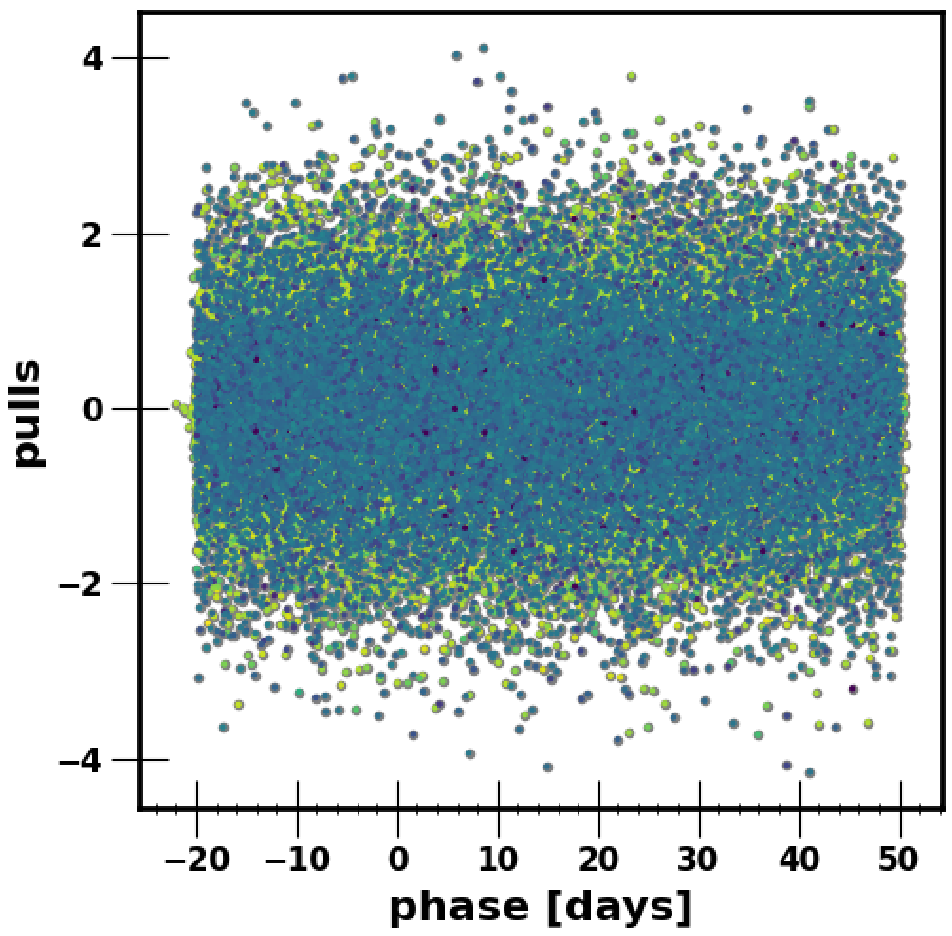
\includegraphics[width=0.5\textwidth]{MainLayout/DC_chapter/figures/new_fig/lc_pulls.png}
    \caption{Photometric pulls as a function of phase for one 
    realization of pre-DC1. The pulls are centred around zero 
    across the full phase range.}
    \label{fig:dc1_lc_pulls}
\end{figure}

\begin{figure}[ht]
    \centering
    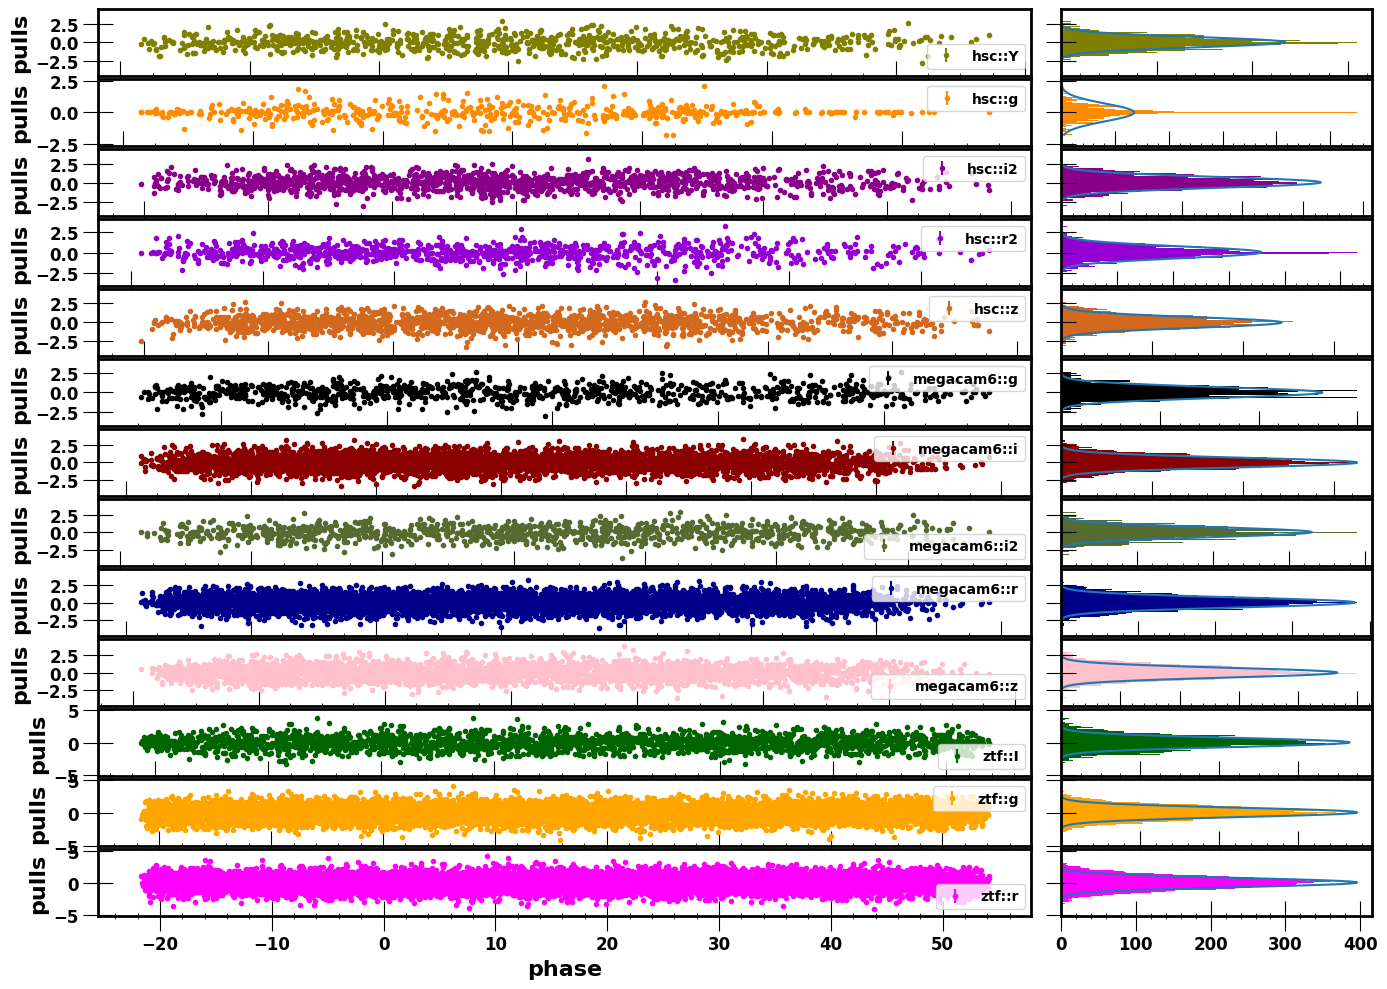
\includegraphics[width=1\textwidth]{MainLayout/DC_chapter/figures/new_fig/lc_pulls_per_band.png}
    \caption{\textit{Left}: Photometric pulls per band for one 
    realization of pre-DC1. \textit{Right}: Histogram of the pulls 
    per band, each fitted with a Gaussian (solid line). The fitted 
    means are consistent with zero.}
    \label{fig:dc1_lc_band_resid}
\end{figure}

\begin{figure}[ht]
    \centering
    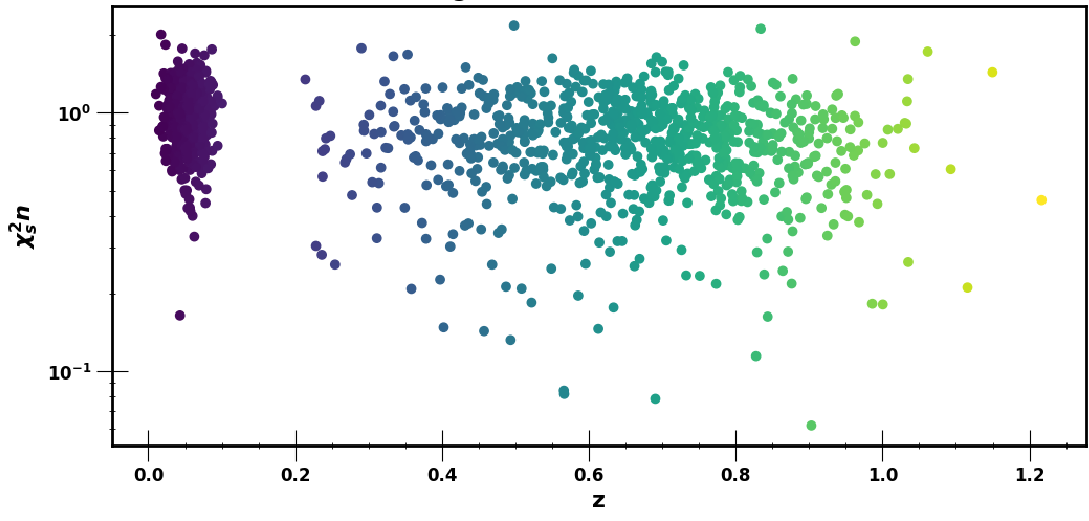
\includegraphics[width=0.8\textwidth]{MainLayout/DC_chapter/figures/new_fig/lc_chi2_z.png}
    \caption{Photometric $\chi^2_{\text{SN}}$ per supernova as a function 
    of redshift for one realization of pre-DC1.}
    \label{fig:dc1_lc_chi2}
\end{figure}

\begin{figure}[ht]
    \centering
    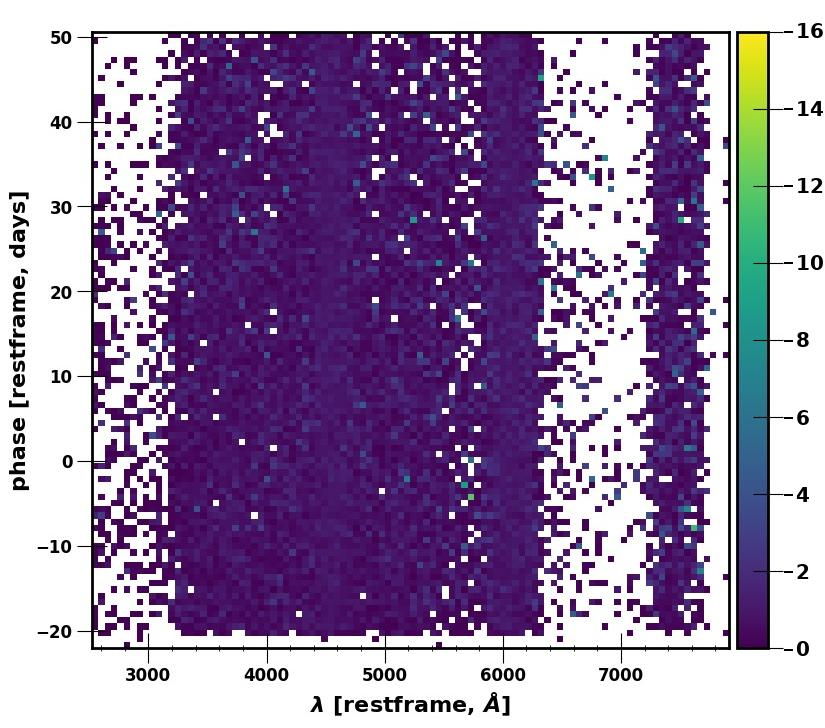
\includegraphics[width=0.8\textwidth]{MainLayout/DC_chapter/figures/new_fig/phot_chi2_edit.jpeg}
    \caption{Stacked photometric $\chi^2_{\text{loc}}$ as a function of phase 
    and wavelength for one realization of pre-DC1.}
    \label{fig:dc1_lc_resid}
\end{figure}

\subsubsection{Spectroscopy}

The spectroscopic analysis yields consistent results. 
Figure 
\ref{fig:dc1_spec_pulls} shows the spectroscopic pulls as a 
function of wavelength. They are centred around zero across 
the full wavelength range. 
Figure \ref{fig:dc1_spec_chi2} shows the supernova $\chi^2_{\text{SN}}$ calculated using the spectroscopic data 
as a function of redshift, which again shows no 
redshift-dependent trend. Figure \ref{fig:dc1_spec_resid} 
shows the stacked $\chi^2_{\text{loc}}$ over wavelength confirming a 
uniformly accurate spectroscopic description.

\begin{figure}[ht]
    \centering
    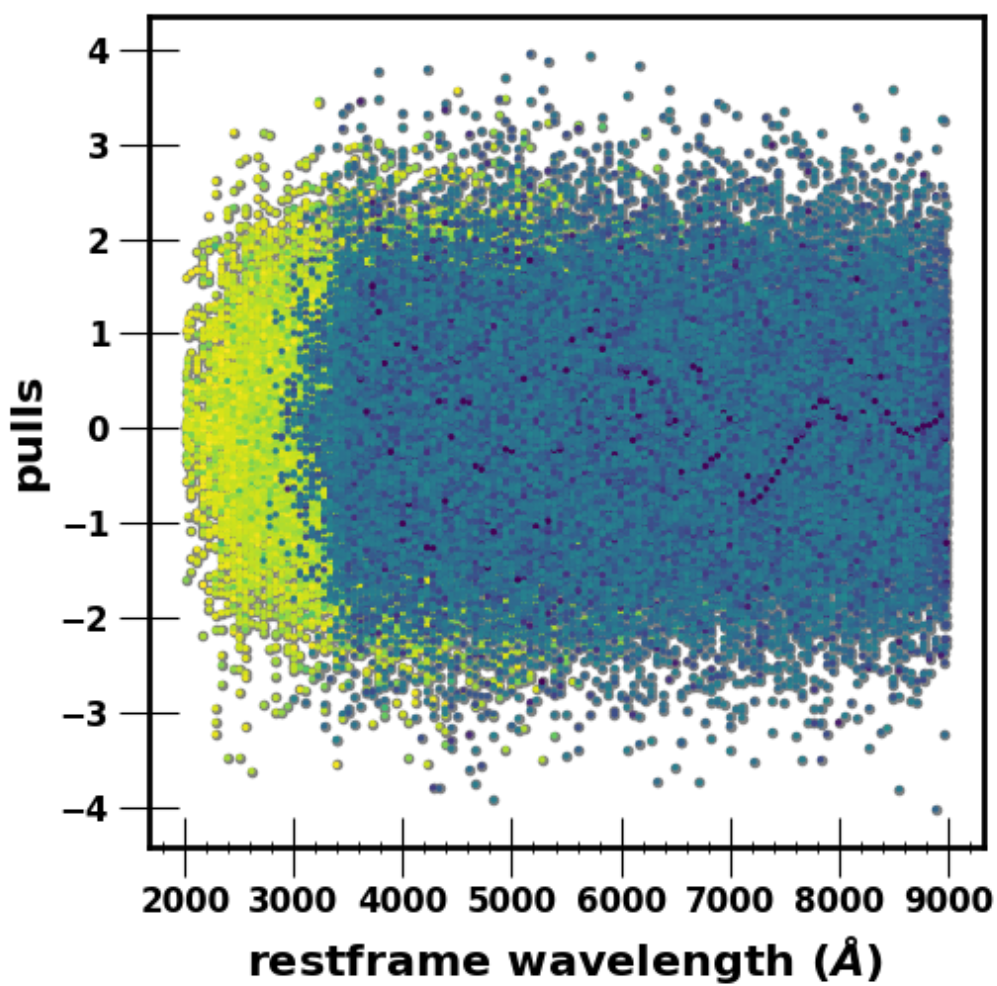
\includegraphics[width=0.5\textwidth]{MainLayout/DC_chapter/figures/new_fig/spec_pulls.png}
    \caption{Spectroscopic pulls as a function of wavelength for 
    one realization of pre-DC1.}
    \label{fig:dc1_spec_pulls}
\end{figure}

\begin{figure}[ht]
    \centering
    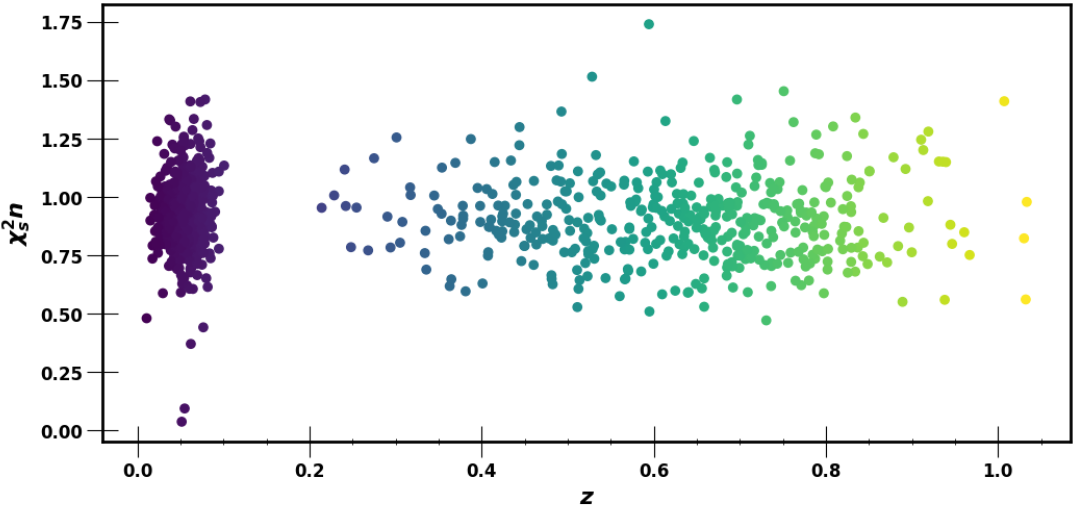
\includegraphics[width=0.8\textwidth]{MainLayout/DC_chapter/figures/new_fig/spec_chi2_z.png}
    \caption{Spectroscopic $\chi^2$ per supernova as a 
    function of redshift for one realization of pre-DC1.}
    \label{fig:dc1_spec_chi2}
\end{figure}

\begin{figure}[ht]
    \centering
    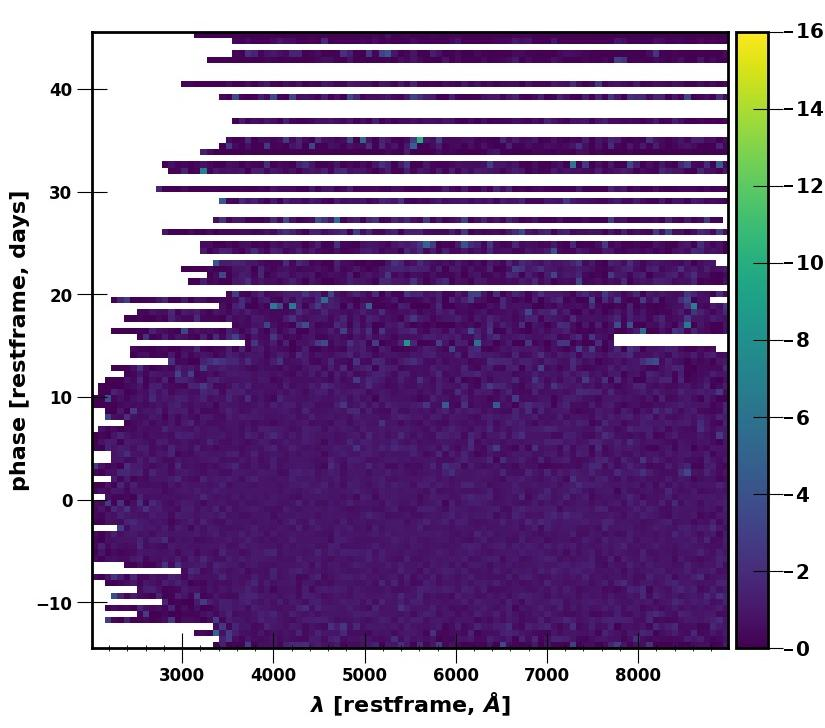
\includegraphics[width=0.8\textwidth]{MainLayout/DC_chapter/figures/new_fig/spec_chi2_edit.jpeg}
    \caption{Stacked spectroscopic $\chi^2$ as a function of 
    wavelength for one realization of pre-DC1.}
    \label{fig:dc1_spec_resid}
\end{figure}



\subsection{Parameter Reconstruction and Covariance Matrix}

Since the pre-DC1 dataset is generated with a model that respects NaCl constraints, we expect to reconstruct the exact same parameters used in the generation. 
In Figure \ref{fig:sn_pars_wres} we compare the generated and reconstructed $X_0$, $X_1$, $c$ and $t_{max}$ parameters averaged over all 100 realizations of pre-DC1. 
This is done by calculating the pulls for each parameter. This is observed as a function of redshift 
to verify whether NaCl introduces redshift-dependent biases on the supernova parameters. 
We see that the reconstructed parameters match the input parameters within the statistical uncertainties of the reconstruction.\\

\begin{figure}[ht]
    \centering
    %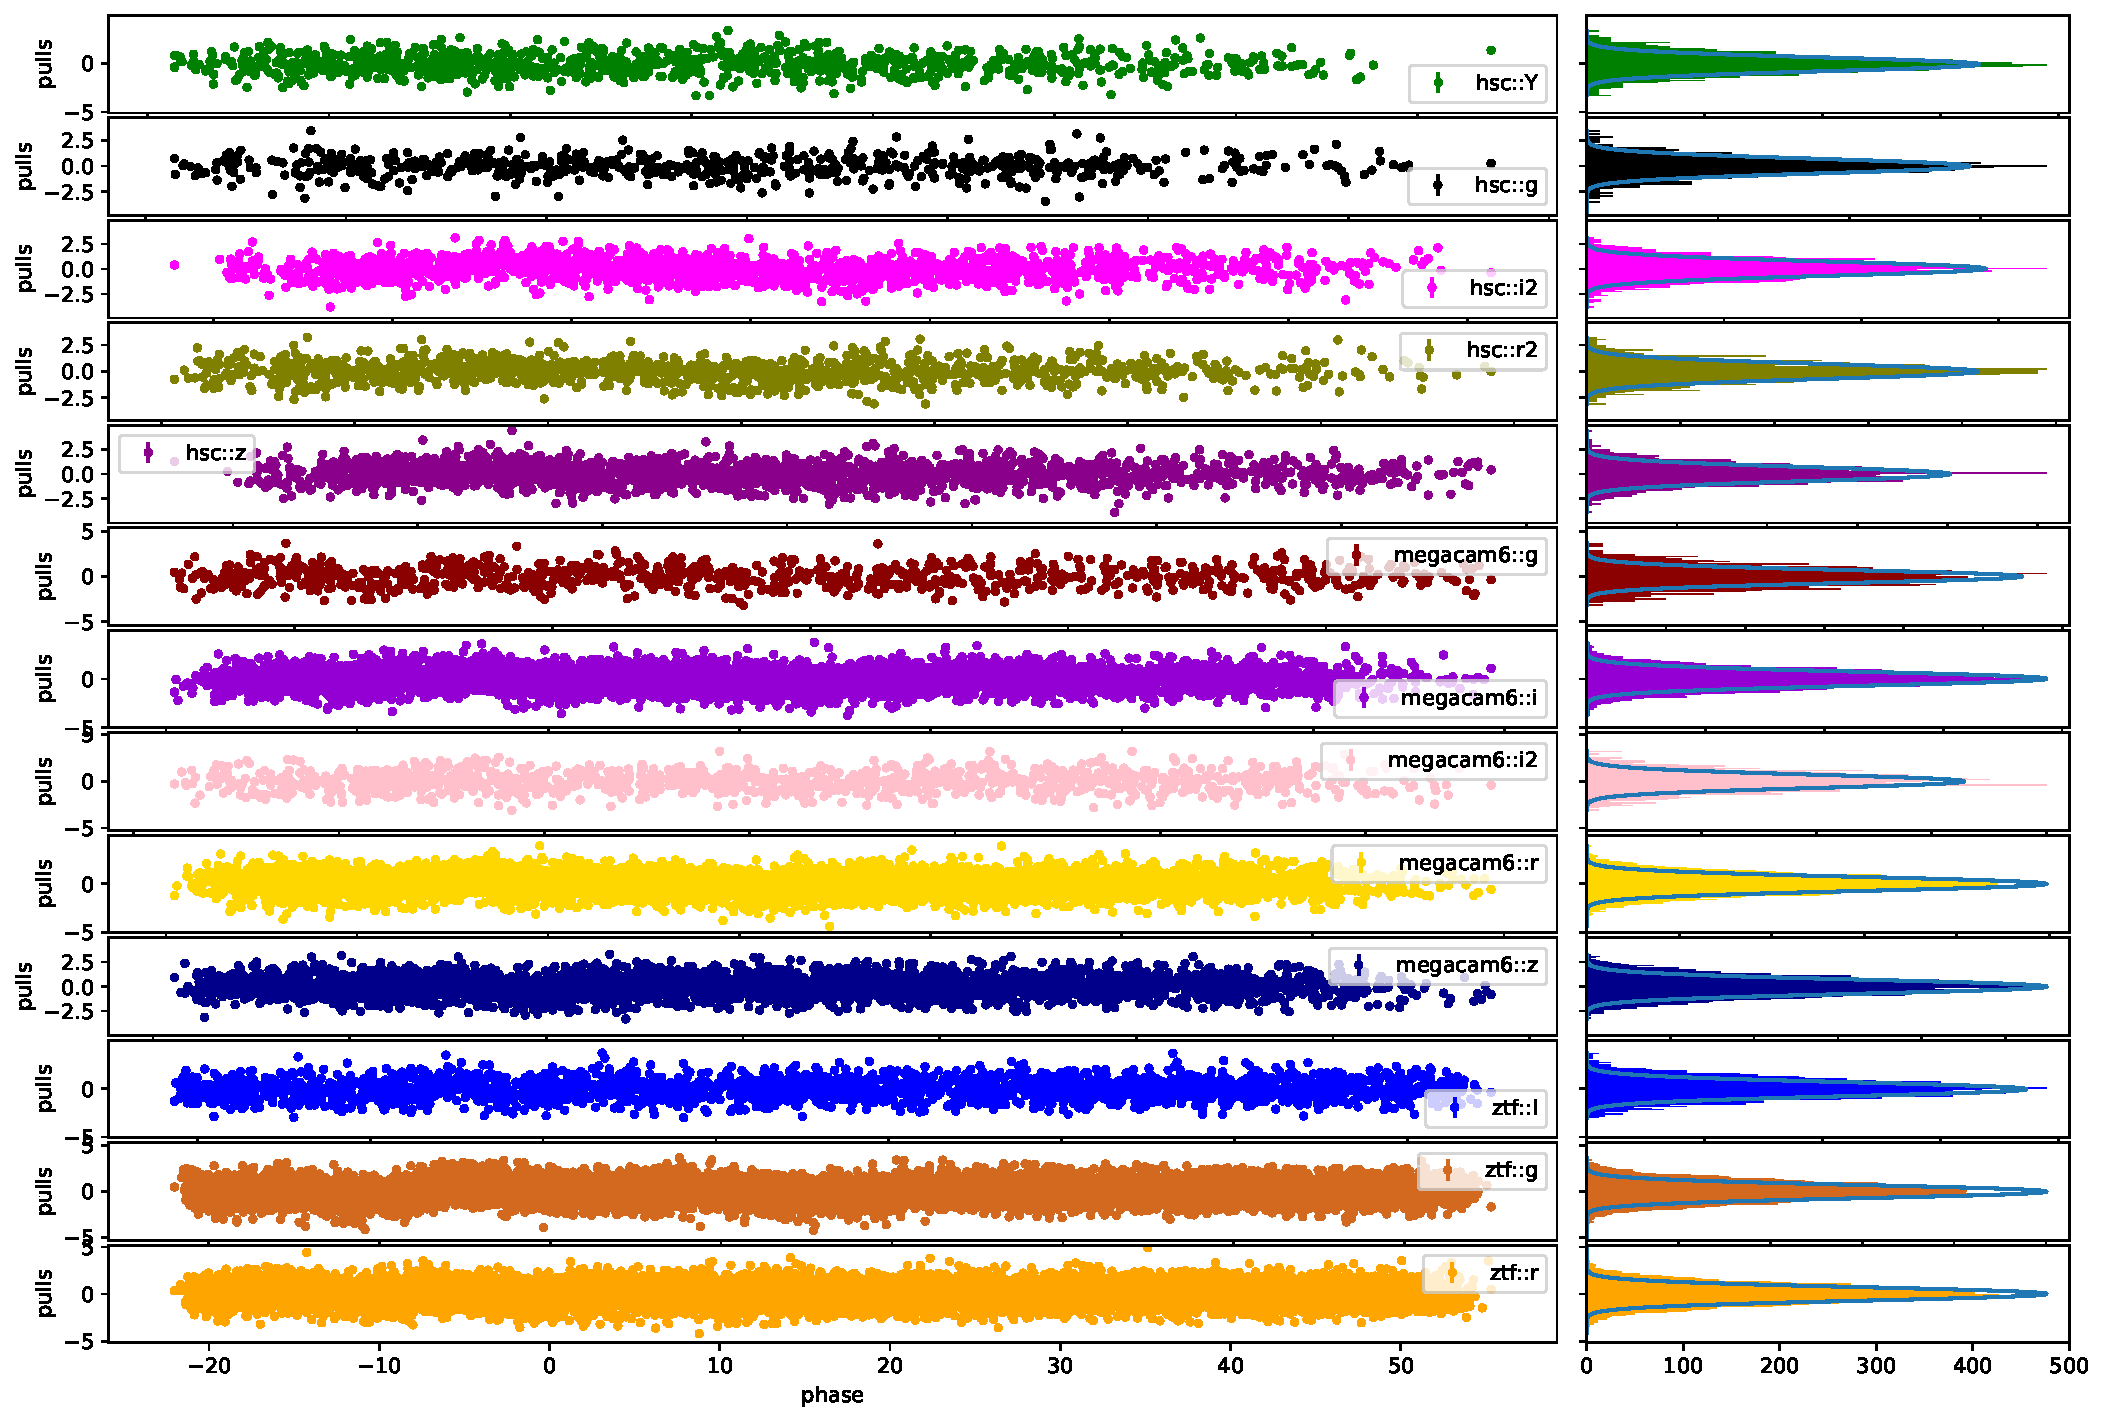
\includegraphics[width=1\textwidth]{MainLayout/DC_chapter/figures/band_resid.pdf}
    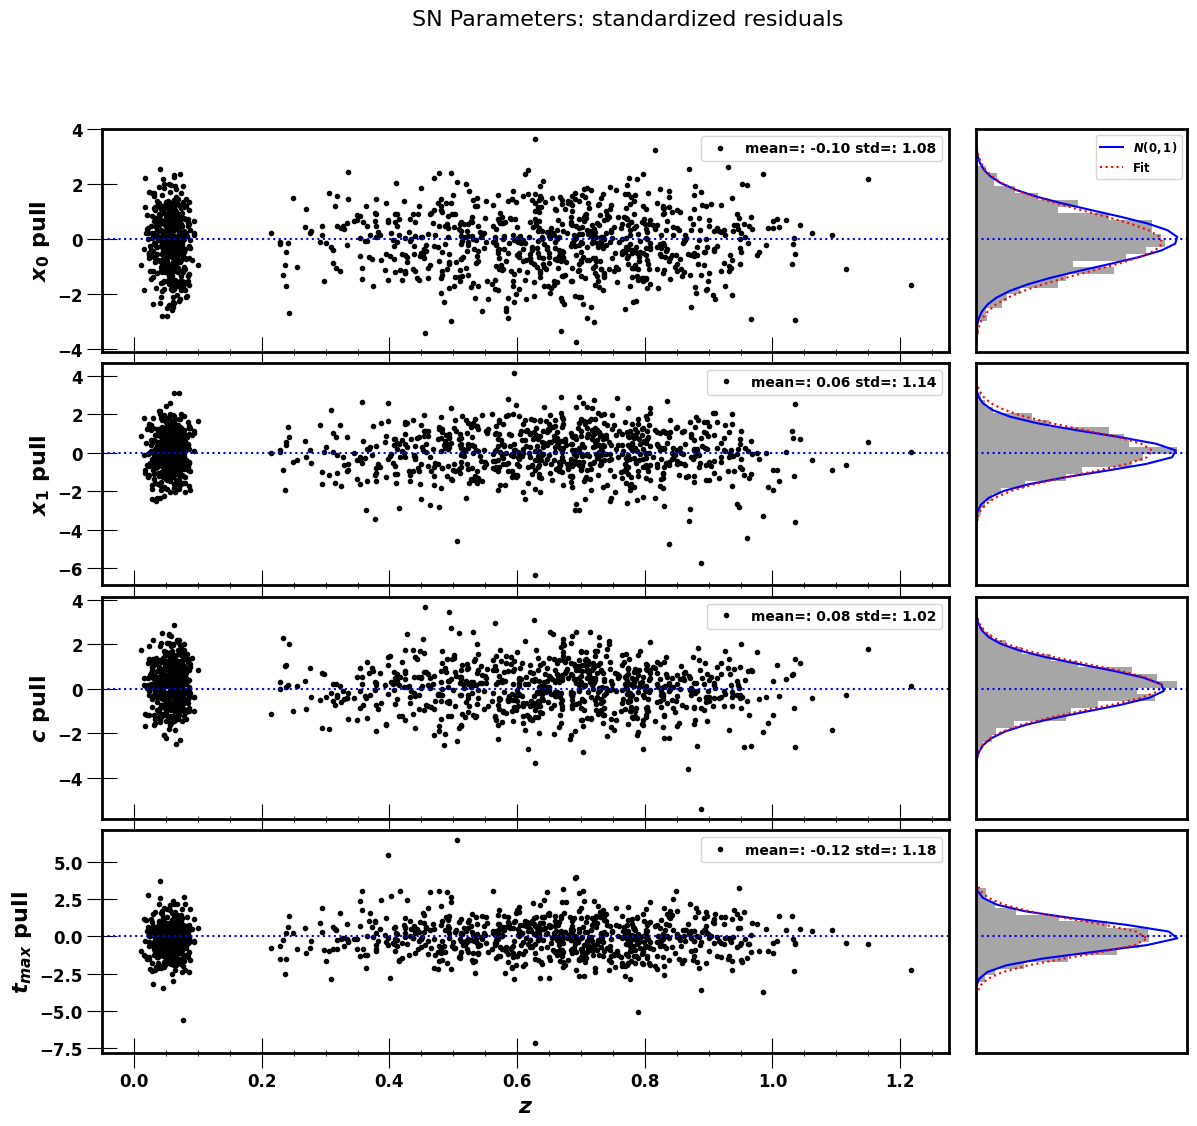
\includegraphics[width=1\textwidth]{MainLayout/DC_chapter/figures/new_fig/sn_pars_wres.png}
    \caption{Weighted residuals of each supernova parameter for 100 realizations of pre-DC1}
    \label{fig:sn_pars_wres}
\end{figure}

We are also interested in comparing the constructed empirical covariance matrix and the Fisher covariance matrix from NaCl. In Figure \ref{fig:pars_cov}, we compare the 
output uncertainties $\sigma_{\text{Fisher}}$ from one pre-DC1 realization with the uncertainties extracted from the empirical uncertainties $\sigma_{\text{Emp}}$ constructed from the run 
on the 100 pre-DC1 realizations as a function of redshift. A more visual representation can be seen in Figure \ref{fig:pars_corr} where compare the correlation matrices constructed from the 
Fisher covariance matrix and the empirical covariance matrix. 
We calculate the ratio of $\sigma_{\text{Emp}}$/$\sigma_{\text{Fisher}}$ and we see that for large part the uncertainties 
are near 1 with a preference for the empirical uncertainties to be slightly higher than the uncertainties predicted by the NaCl output. This likely due to the fact that 
100 realizations may not be enough to reconstruct an exact covariance matrix. 
To assess whether 100 realizations are sufficient to estimate the 
empirical covariance, a previous iteration of pre-DC1 with $\sim 1000$ 
supernovae per realization was used to generate 900 realizations. 
Comparing the empirical covariance constructed from 100 vs 900 
realizations showed that the ratio $\sigma_{\text{Emp}}/\sigma_{\text{Fisher}}$ 
converges toward unity with increasing sample size, confirming that 
the residual excess in the 100-realization estimate is a finite-sample 
effect rather than a systematic bias in the NaCl uncertainty 
propagation. The slight overestimate of $\sigma_{\text{Emp}}$ relative 
to $\sigma_{\text{Fisher}}$ seen in Figure \ref{fig:pars_cov} is 
therefore not a cause for concern.


\begin{figure}[ht]
    \centering
    %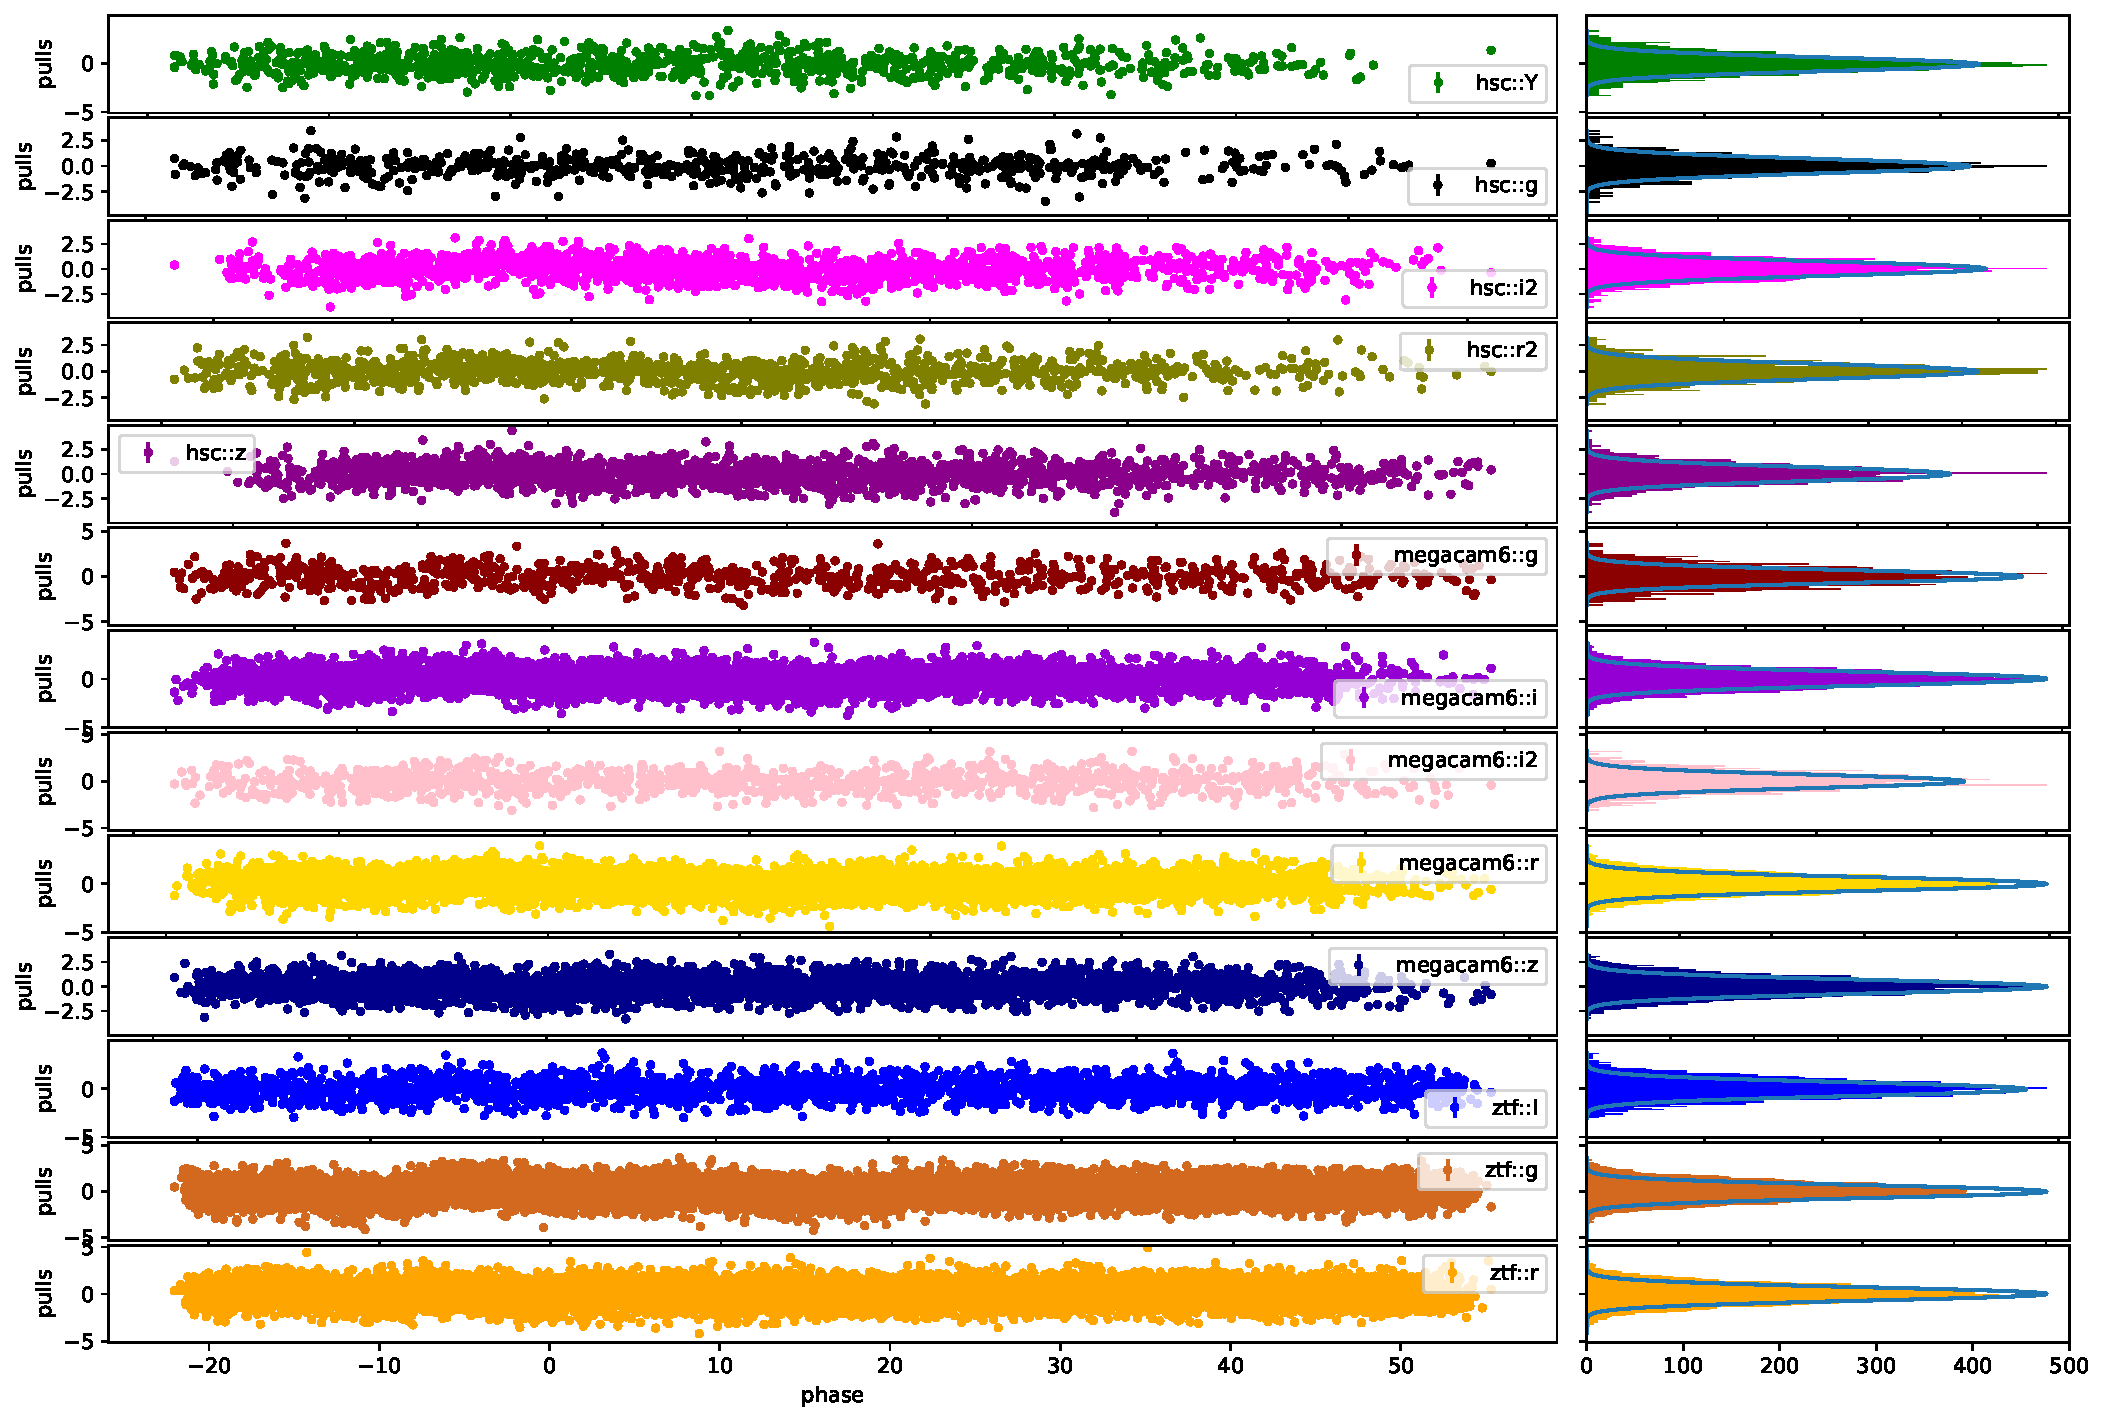
\includegraphics[width=1\textwidth]{MainLayout/DC_chapter/figures/band_resid.pdf}
    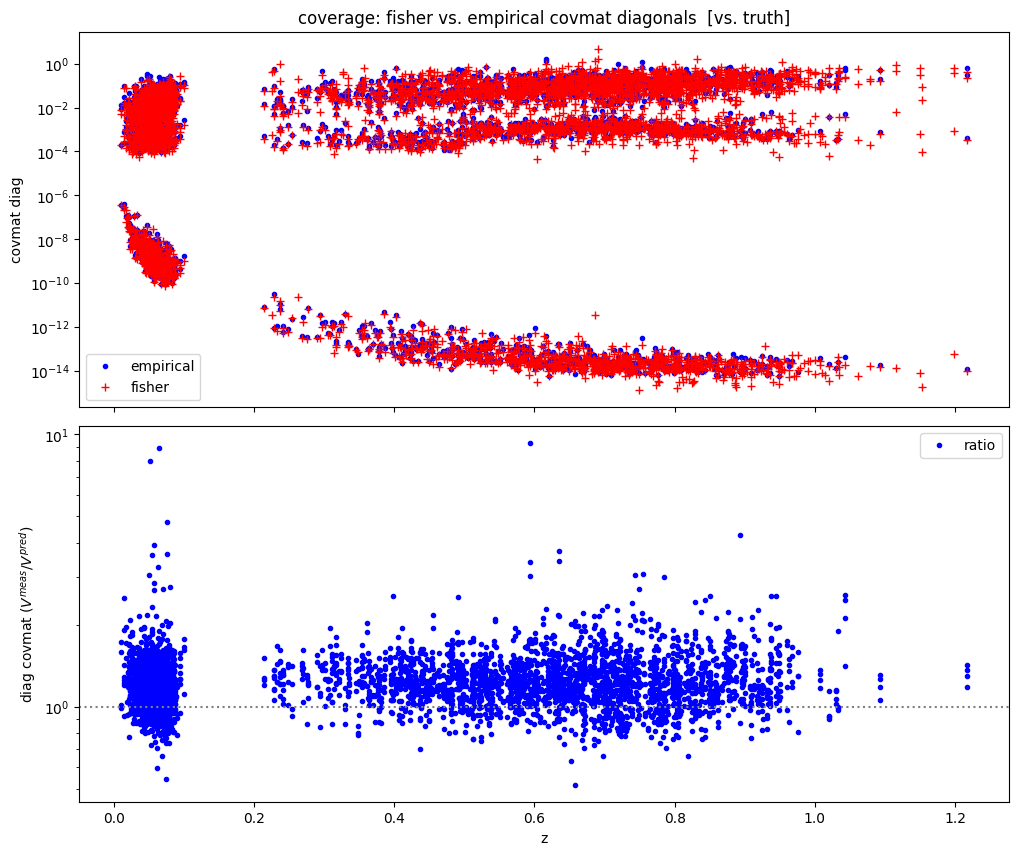
\includegraphics[width=0.8\textwidth]{MainLayout/DC_chapter/figures/new_fig/coverage_all.png}
    \caption{\textit{Top}: $\sigma_{\text{Fisher}}$ in red cross and $\sigma_{\text{Emp}}$ blue dots as a function of redshift. We see distinct layers in the uncertainties that are related 
    to the different parameters $X_0$, $X_1$, $c$ and $t_{max}$. \textit{Bottom}: Ratio of the $\sigma_{\text{Emp}}$ and $\sigma_{\text{Fisher}}$.}
    \label{fig:pars_cov}
\end{figure}


\begin{figure}[ht]
    \centering
    %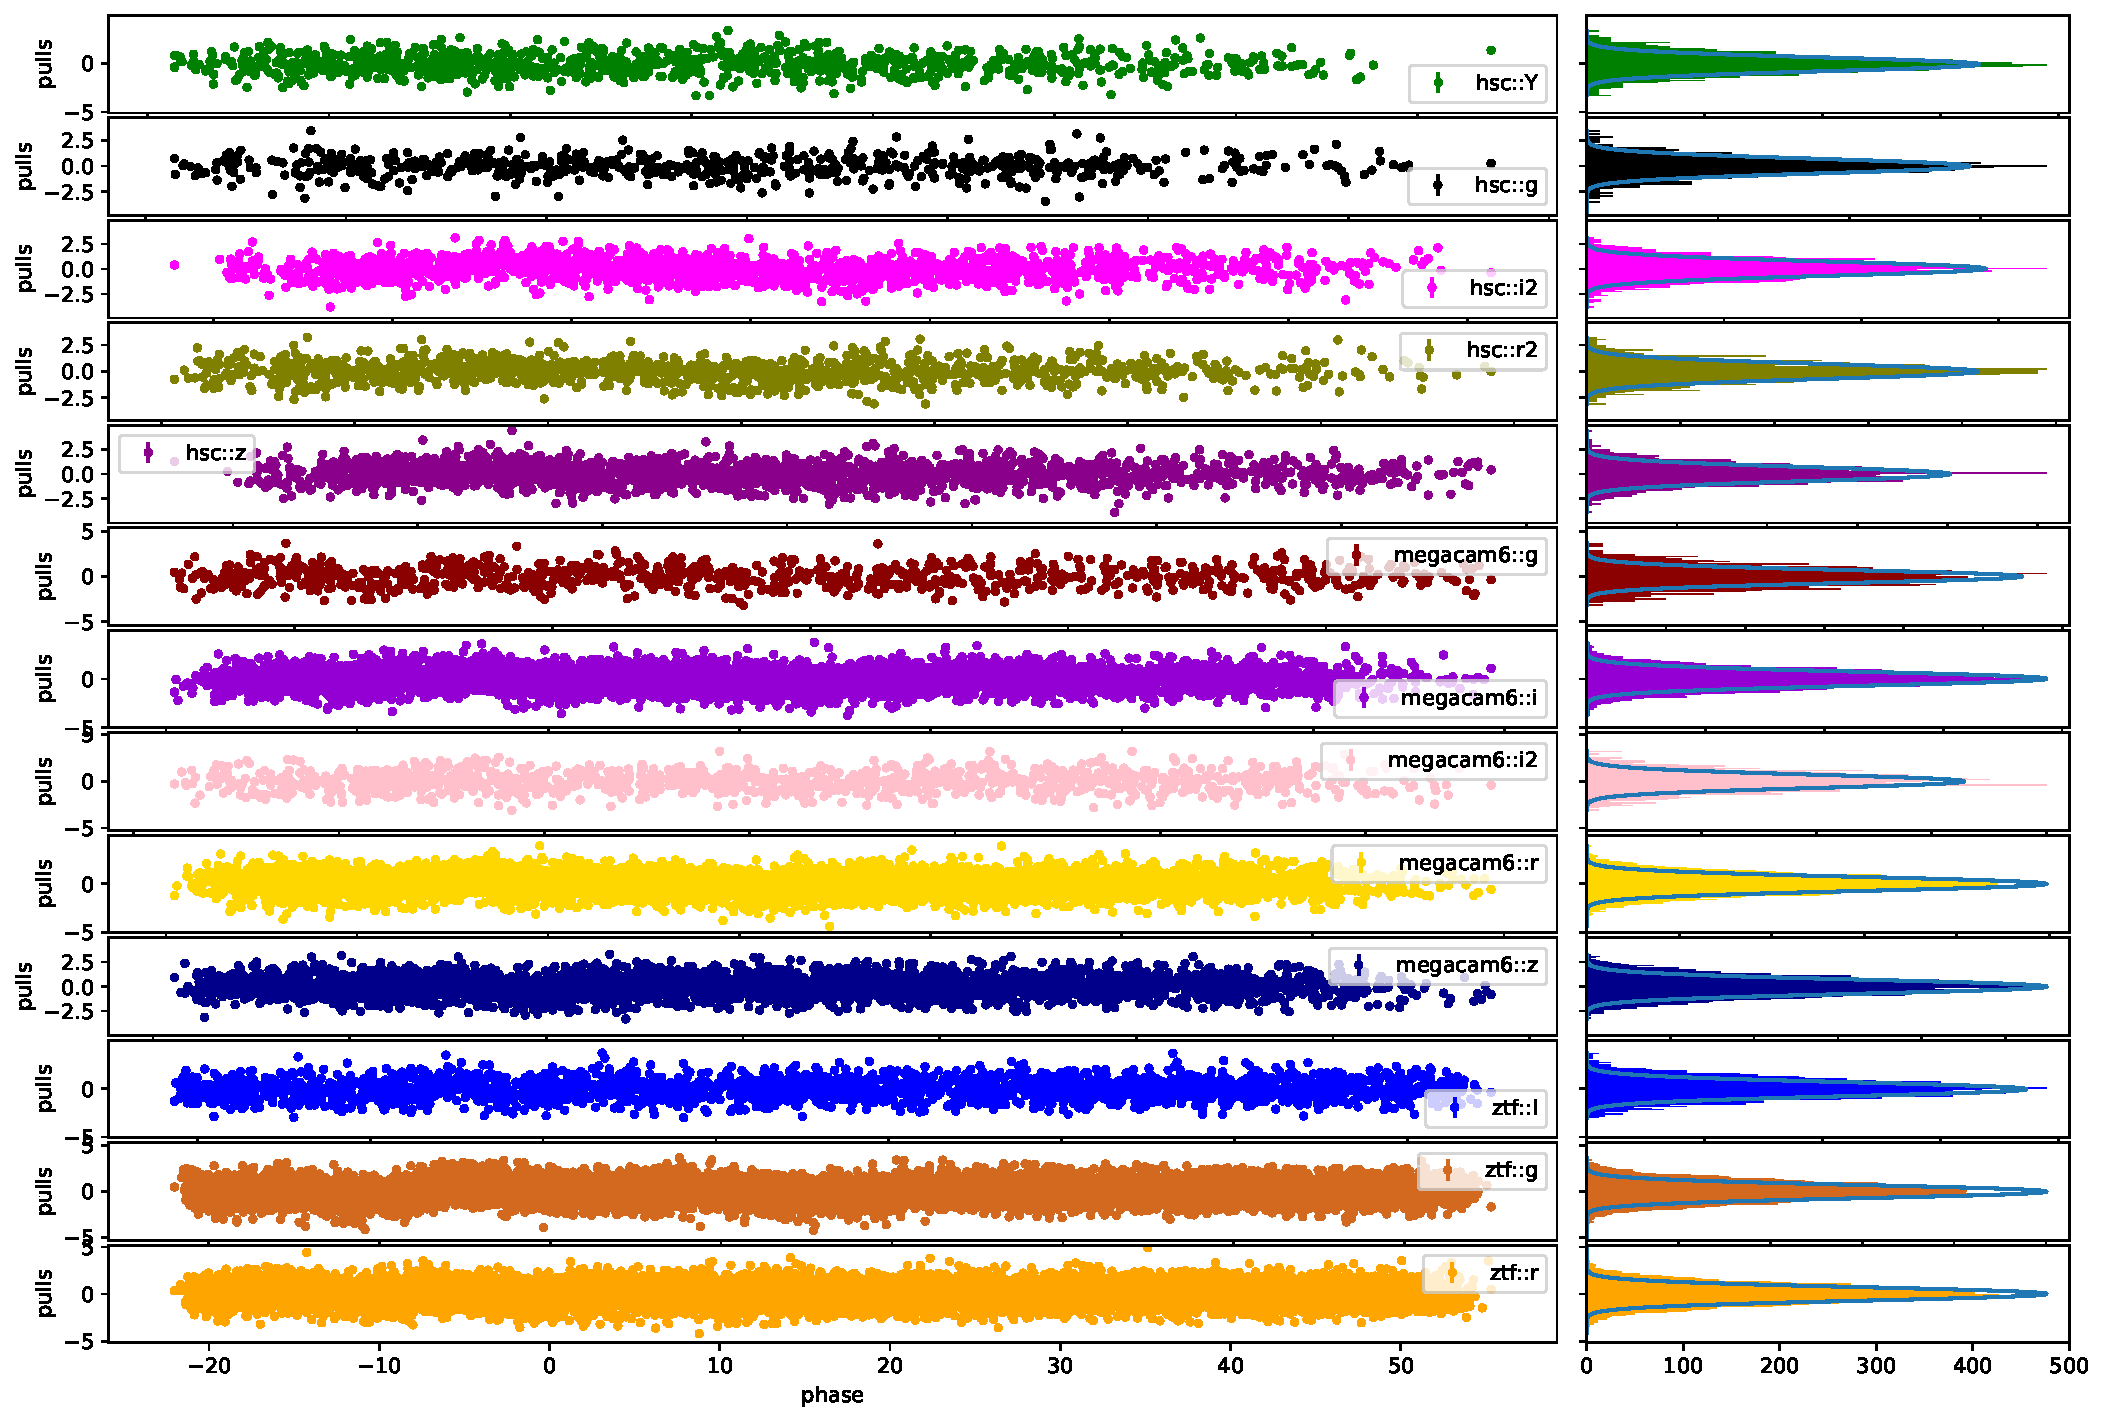
\includegraphics[width=1\textwidth]{MainLayout/DC_chapter/figures/band_resid.pdf}
    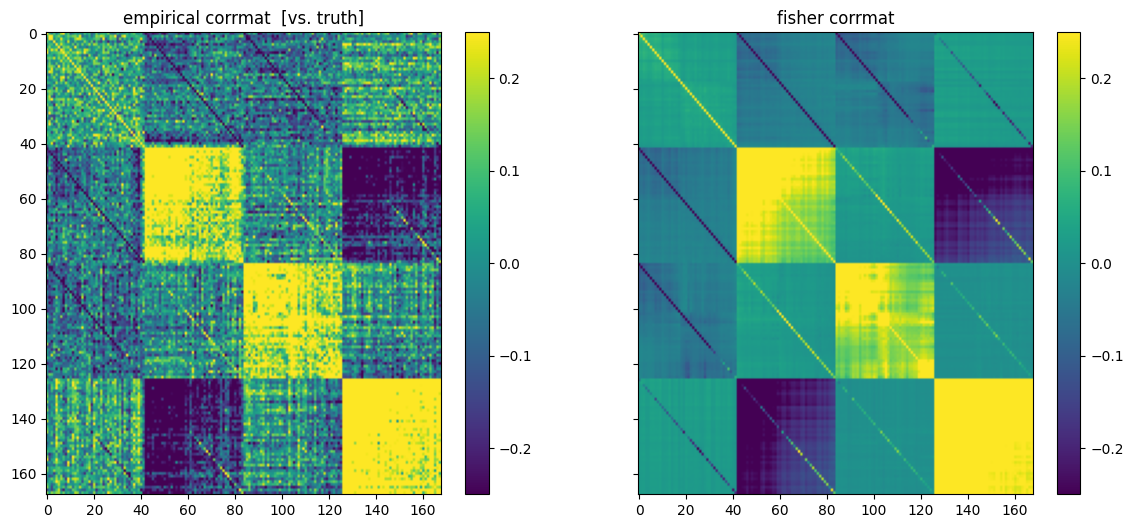
\includegraphics[width=1\textwidth]{MainLayout/DC_chapter/figures/new_fig/corrmats.png}
    \caption{Empirical correlation matrix on the left constructed from the 100 realizations of pre-DC1. Fisher correlation matrix on the right from output of NaCl.}
    \label{fig:pars_corr}
\end{figure}



\subsection{Distance modulus and cosmological parameters reconstruction}

We use EDRIS to determine the distance modulus of the supernovae at the end of the full model training with NaCl. It is important to note
that we are not assessing the efficiency of EDRIS in reconstructing distances as this has already been established in D. Kuhn's 
PhD thesis\footnote{\url{https://theses.hal.science/tel-05451069}} where it was shown that EDRIS does not bias supernova distances in our setup. 
\\

\noindent The results in Figure \ref{fig:pre_dc1_hubble_tot} show the mean binned distance residuals from 100 realizations of pre-DC1 as well as a comparison between
the empirical uncertainties on the binned distances and the Fisher uncertainties from EDRIS. 
We notice significant biases in the mean distance residuals up to $\sim 9$ standard deviations near 
$z \approx 0.1$ and $z \approx 1$, corresponding to the survey 
transition regions between ZTF and SNLS, and at the end of the SNLS and HSC 
surveys. 
The origin of these biases has not yet been conclusively established. 
One possibility is that the model regularization is insufficient, allowing 
artifacts to develop in the reconstructed model and subsequently bias the inferred distances. 
Another possibility is that the quality cuts introduce an effective selection effect. 
Although no explicit selection effects were included in the simulations, these cuts preferentially remove 
some supernovae and may therefore modify the properties of the resulting sample in a way that contributes to the observed bias.\\

\begin{figure}[ht]
    \centering
    %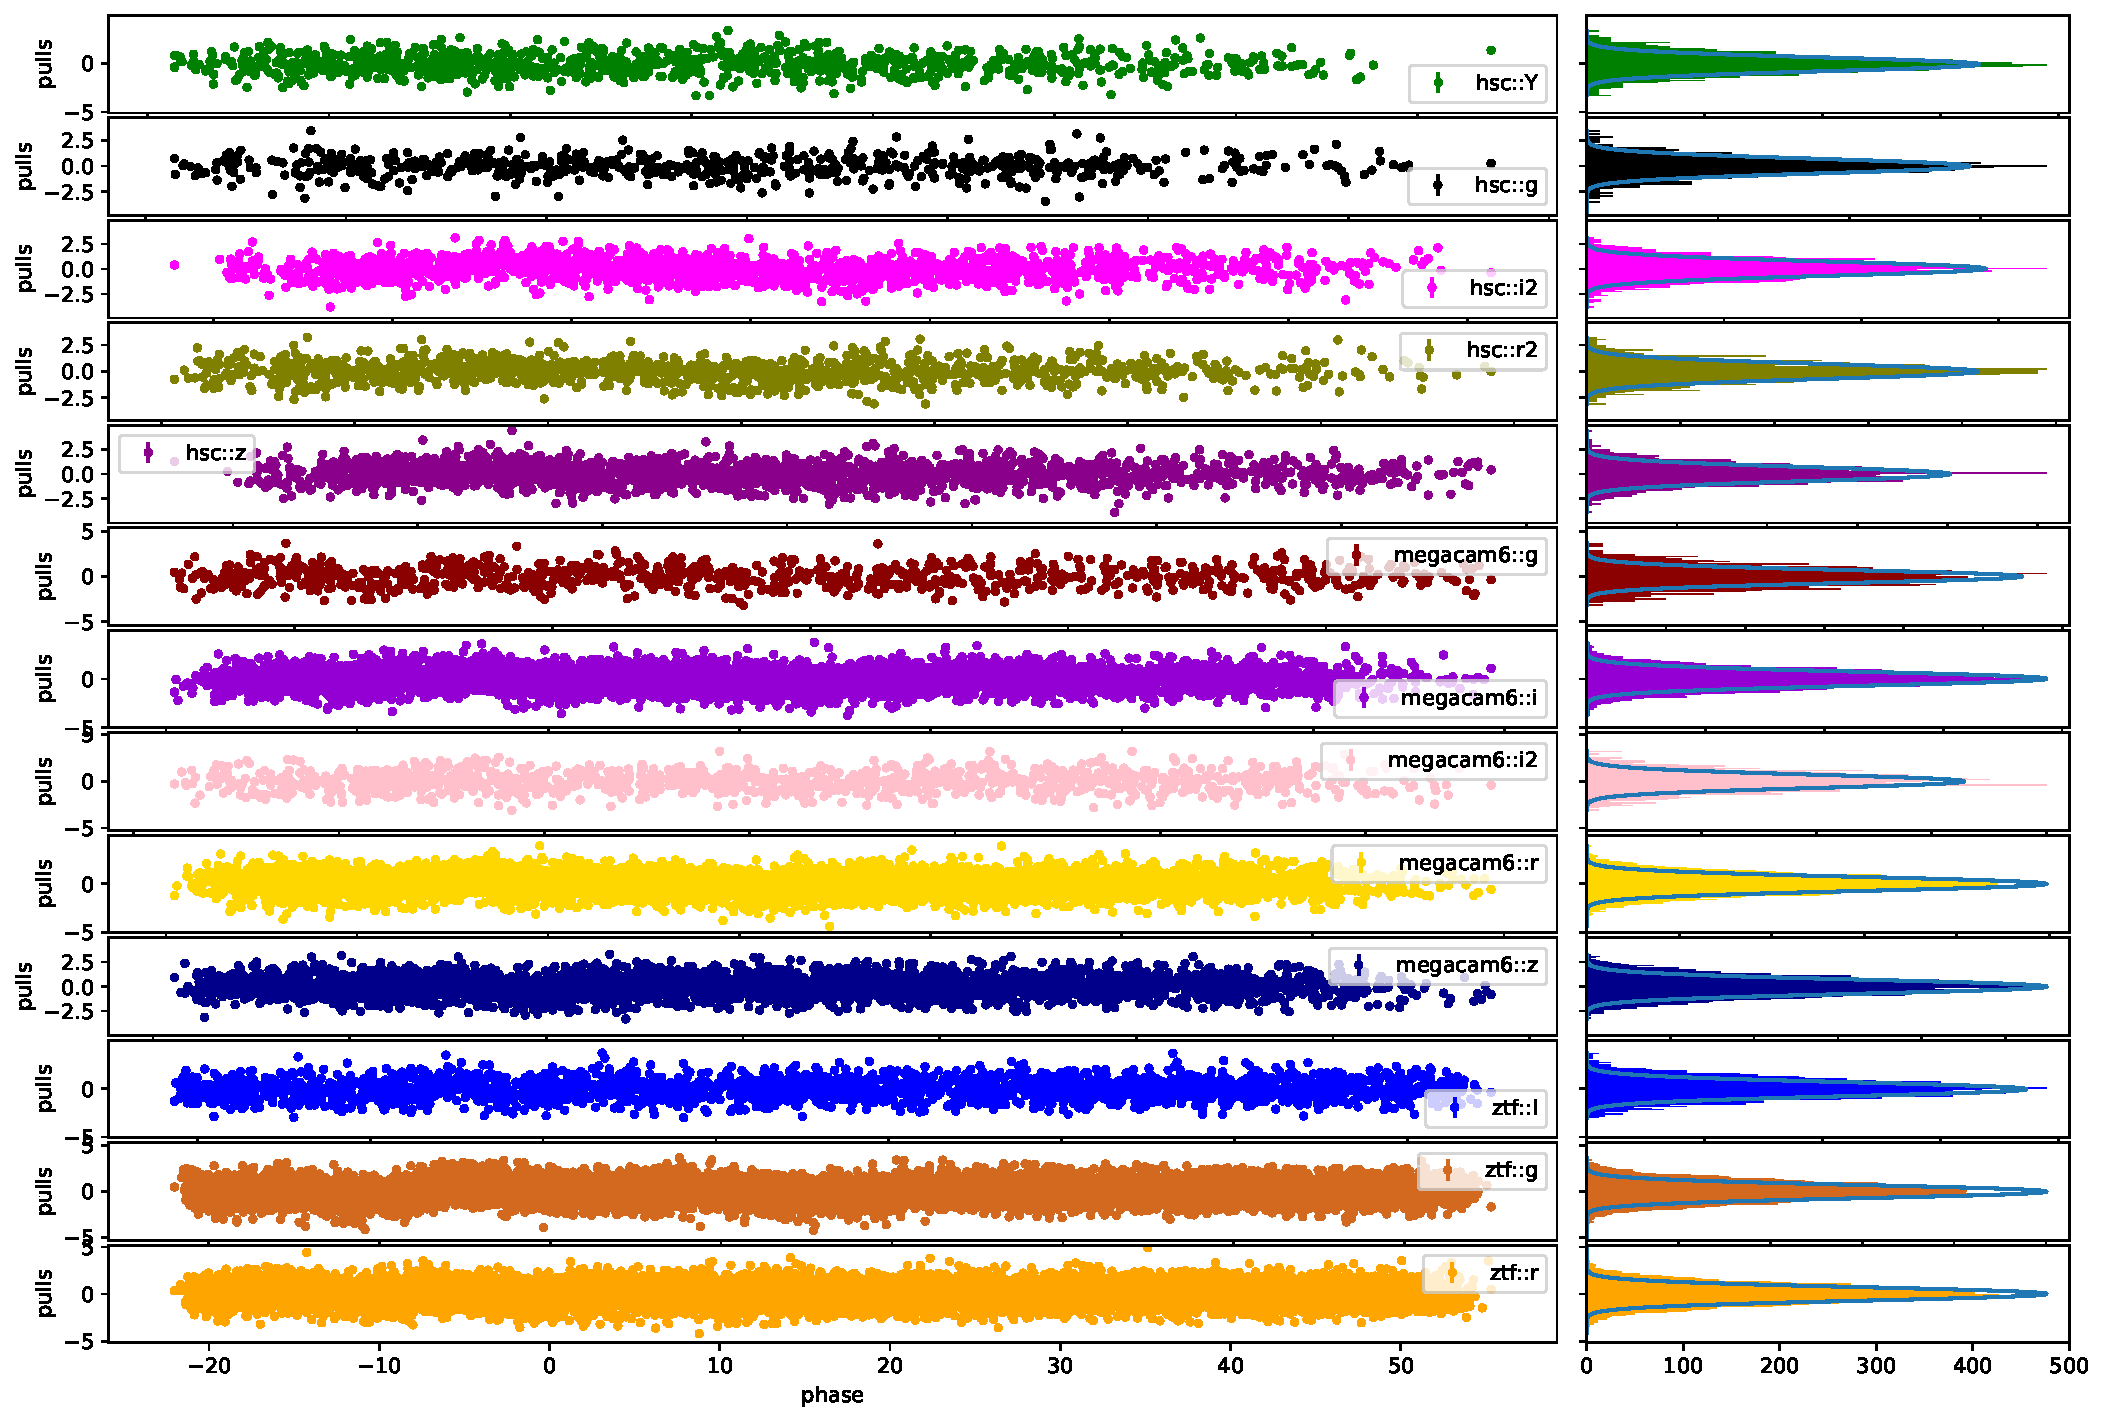
\includegraphics[width=1\textwidth]{MainLayout/DC_chapter/figures/band_resid.pdf}
    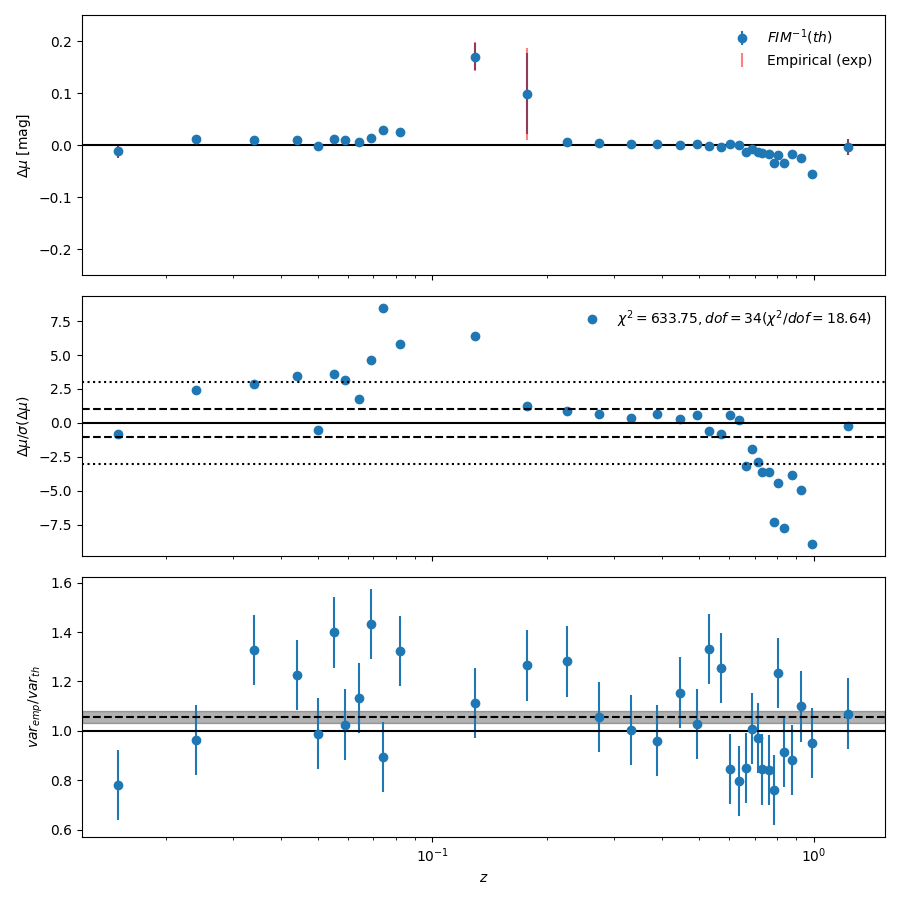
\includegraphics[width=0.8\textwidth]{MainLayout/DC_chapter/figures/new_fig/binned_distances.png}
    \caption{\textit{Top}: Mean of the differences between the reconstructed distance moduli and the truth.
    \textit{Middle}: Weighted residuals of the distance moduli. 
    \textit{Bottom}: Ratio between the empirically constructed variance from EDRIS with the predicted variance. }
    \label{fig:pre_dc1_hubble_tot}
\end{figure}


\noindent 
The \textsc{Lemaître} pipeline outputs constraints on 
$\Omega_{bc} = \Omega_b + \Omega_c$, the combined baryon and cold 
dark matter density parameter. The neutrino mass is fixed to 
its Planck 2018 minimal mass value and the 
neutrino density parameter $\Omega_\nu$ is small compared to $\Omega_{bc}$ (less than 5\% contributtion to $\Omega_m$)
and therefore approximate $\Omega_m \approx \Omega_{bc}$. 
Results from \texttt{cosmologix} are shown in Figure \ref{fig:dc1_contour} where we show the $\Omega_m$-$w$ contours for six randomly selected individual 
realizations of pre-DC1. We see that amongst them are realizations that we recover the input cosmological parameters within 1 standard deviation while others show significant deviations. 
The distribution of the recovered $\Omega_m$-$w$ parameters from the 100 realizations is seen Figure \ref{fig:w_om_dist}. 

Across the 100 realizations, we find strong biases in the recovered cosmological parameters, with the mean values of $\Omega_m$ and $w$ displaced from their input values by
$15.5 \sigma$ and $10.4 \sigma$ respectively. 
This bias persists when fixing  $w=-1$ and fitting only for $\Omega_m$ for which the recovered mean is displaced from the input value by $19.4 \sigma$ as seen in Figure \ref{fig:om_dist}.
The origin of this bias is currently unknown, but it is likely related to the biases identified in the reconstructed distance moduli, 
since the cosmological parameters are inferred from these distances. \\

\begin{figure}[ht]
    \centering
    %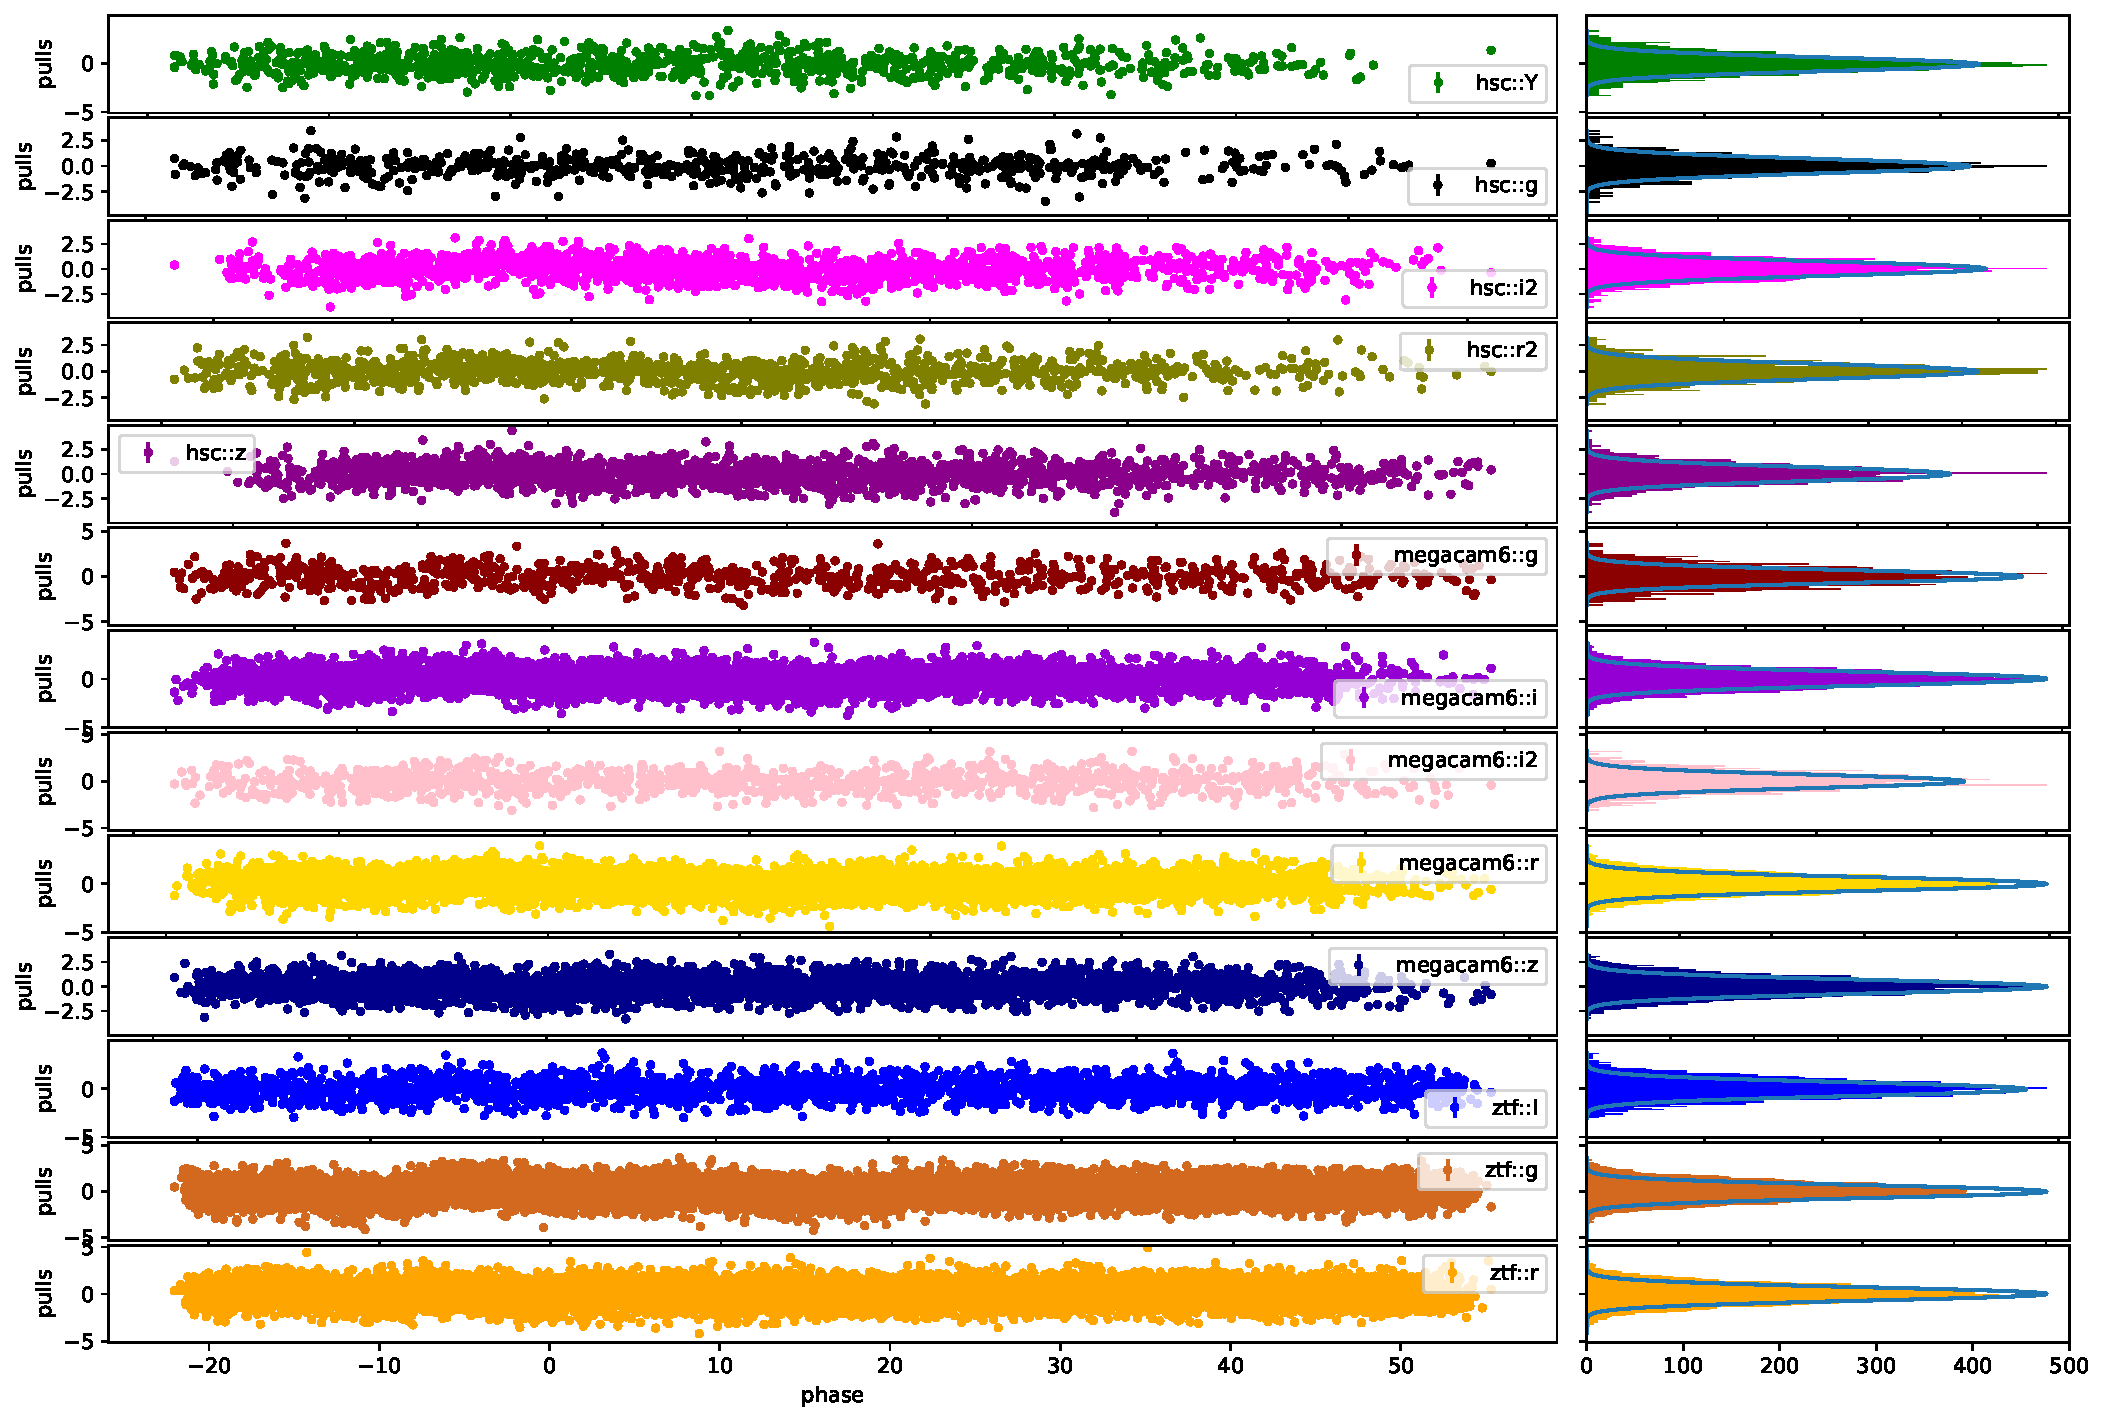
\includegraphics[width=1\textwidth]{MainLayout/DC_chapter/figures/band_resid.pdf}
    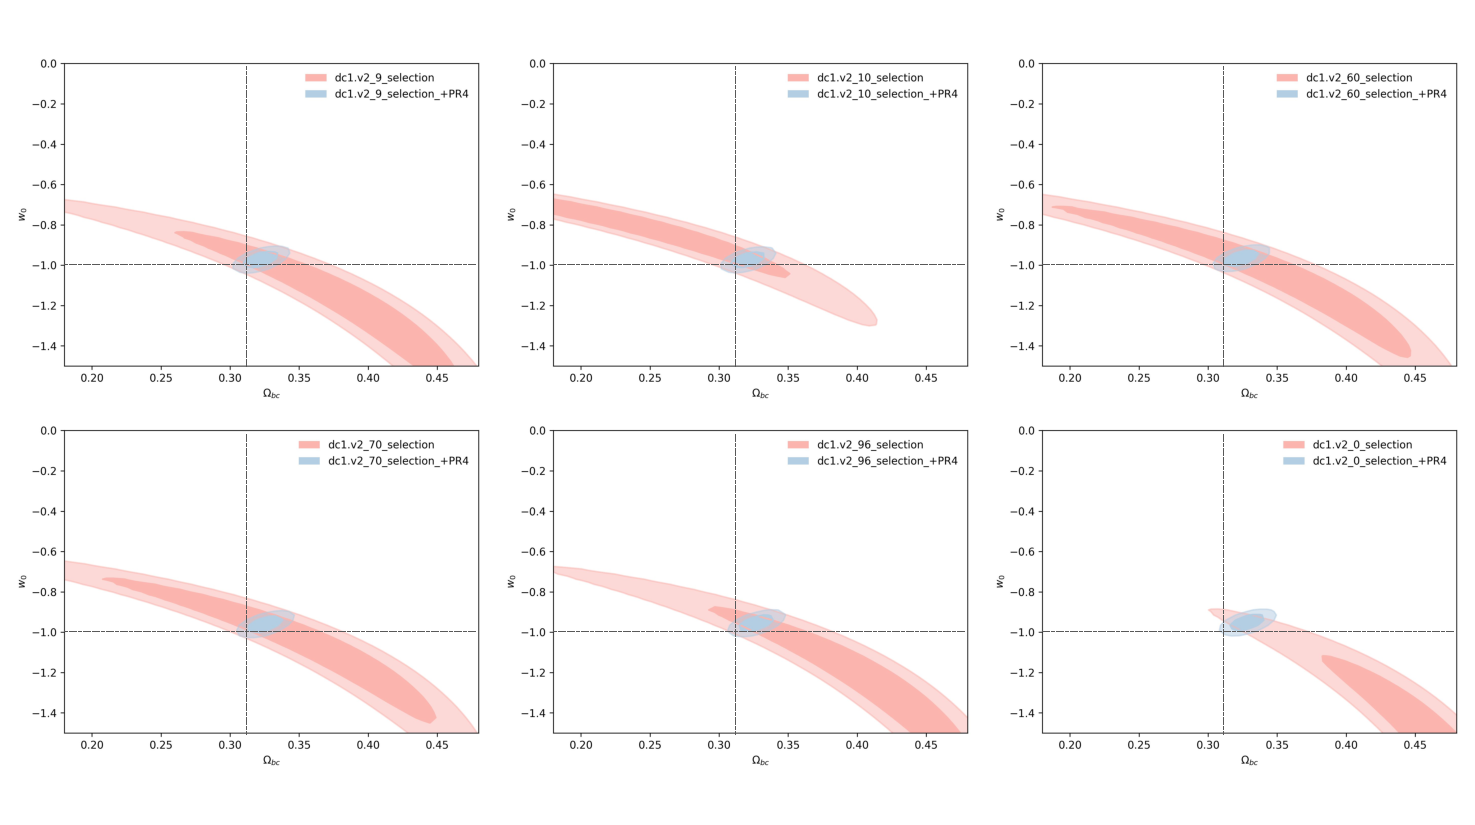
\includegraphics[width=1\textwidth]{MainLayout/DC_chapter/figures/new_fig/contour_comp.pdf}
    \caption{$\Omega_m$-$w$ contours for six realizations of pre-DC1 in the red area. The blue area shows the constraining power when coupled with Planck CMB results.}
    \label{fig:dc1_contour}
\end{figure}

\begin{figure}[ht]
    \centering
    %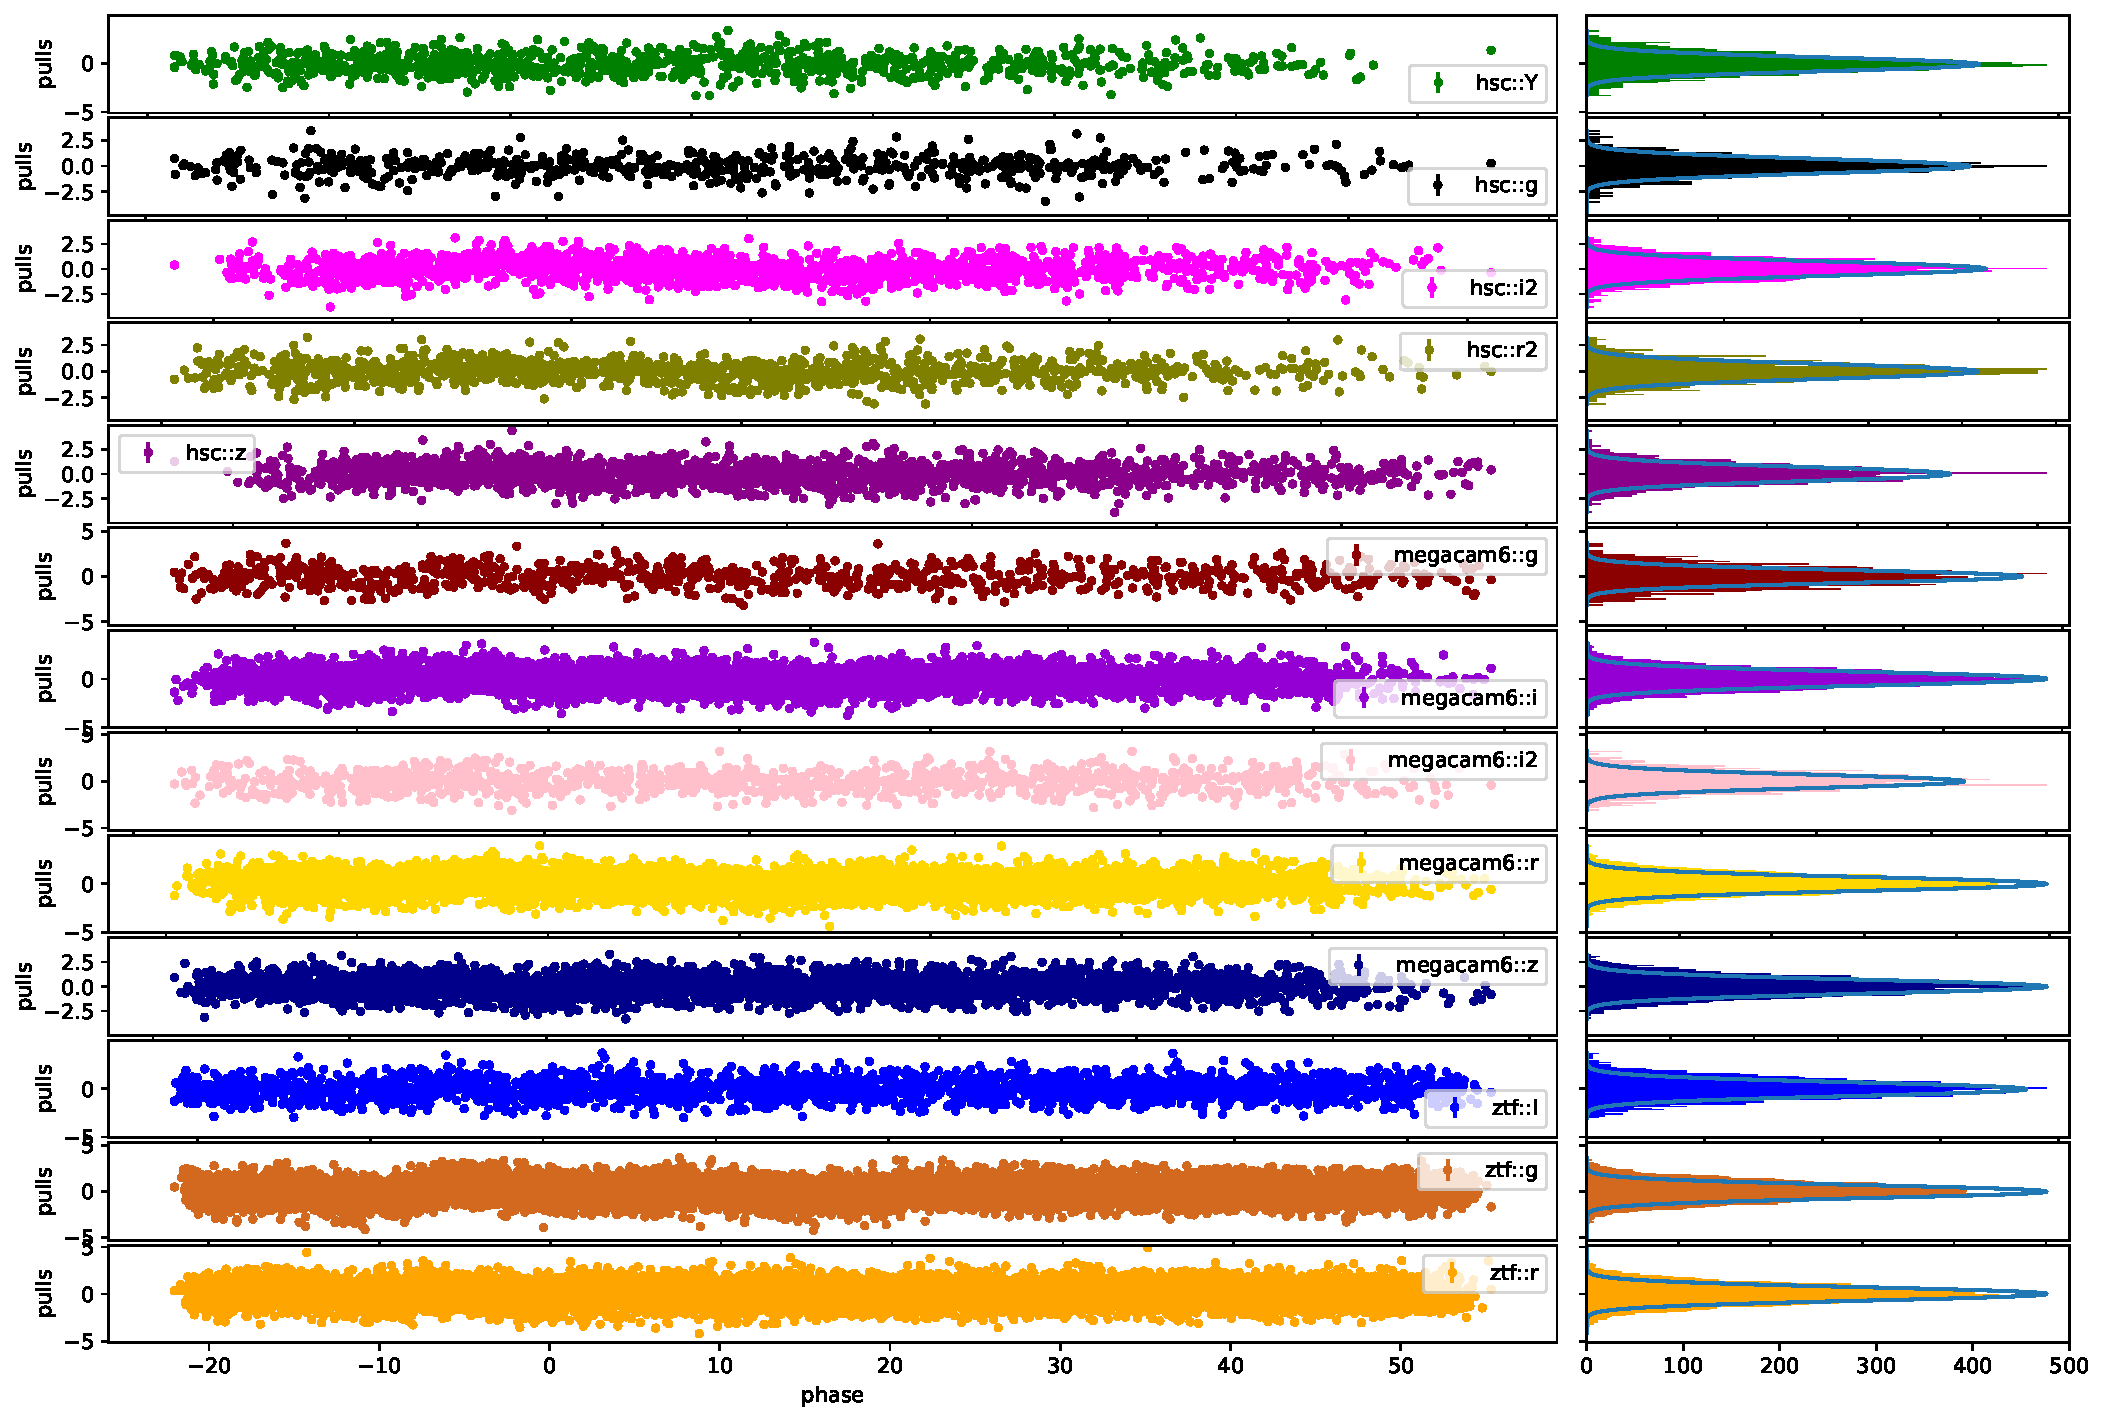
\includegraphics[width=1\textwidth]{MainLayout/DC_chapter/figures/band_resid.pdf}
    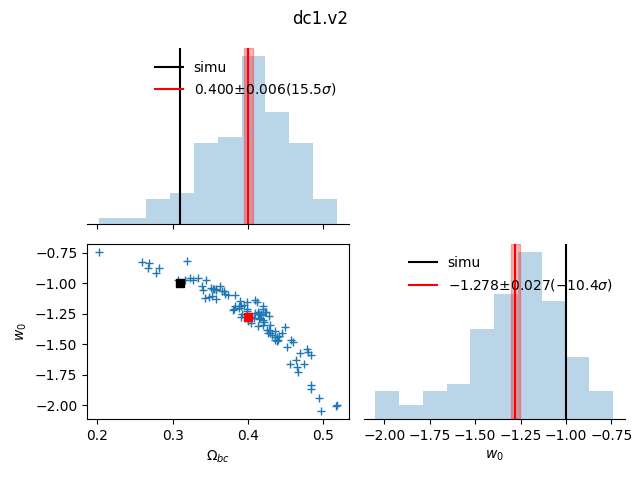
\includegraphics[width=0.8\textwidth]{MainLayout/DC_chapter/figures/new_fig/fwcdm.png}
    \caption{Distribution of $\Omega_m$ and $w$ for the 100 realizations of pre-DC1. The red line represents the mean value of each cosmological parameter as well its 
    standard deviation. The black line represents the expected results used as input for the simulation.}
    \label{fig:w_om_dist}
\end{figure}

\begin{figure}[ht]
    \centering
    %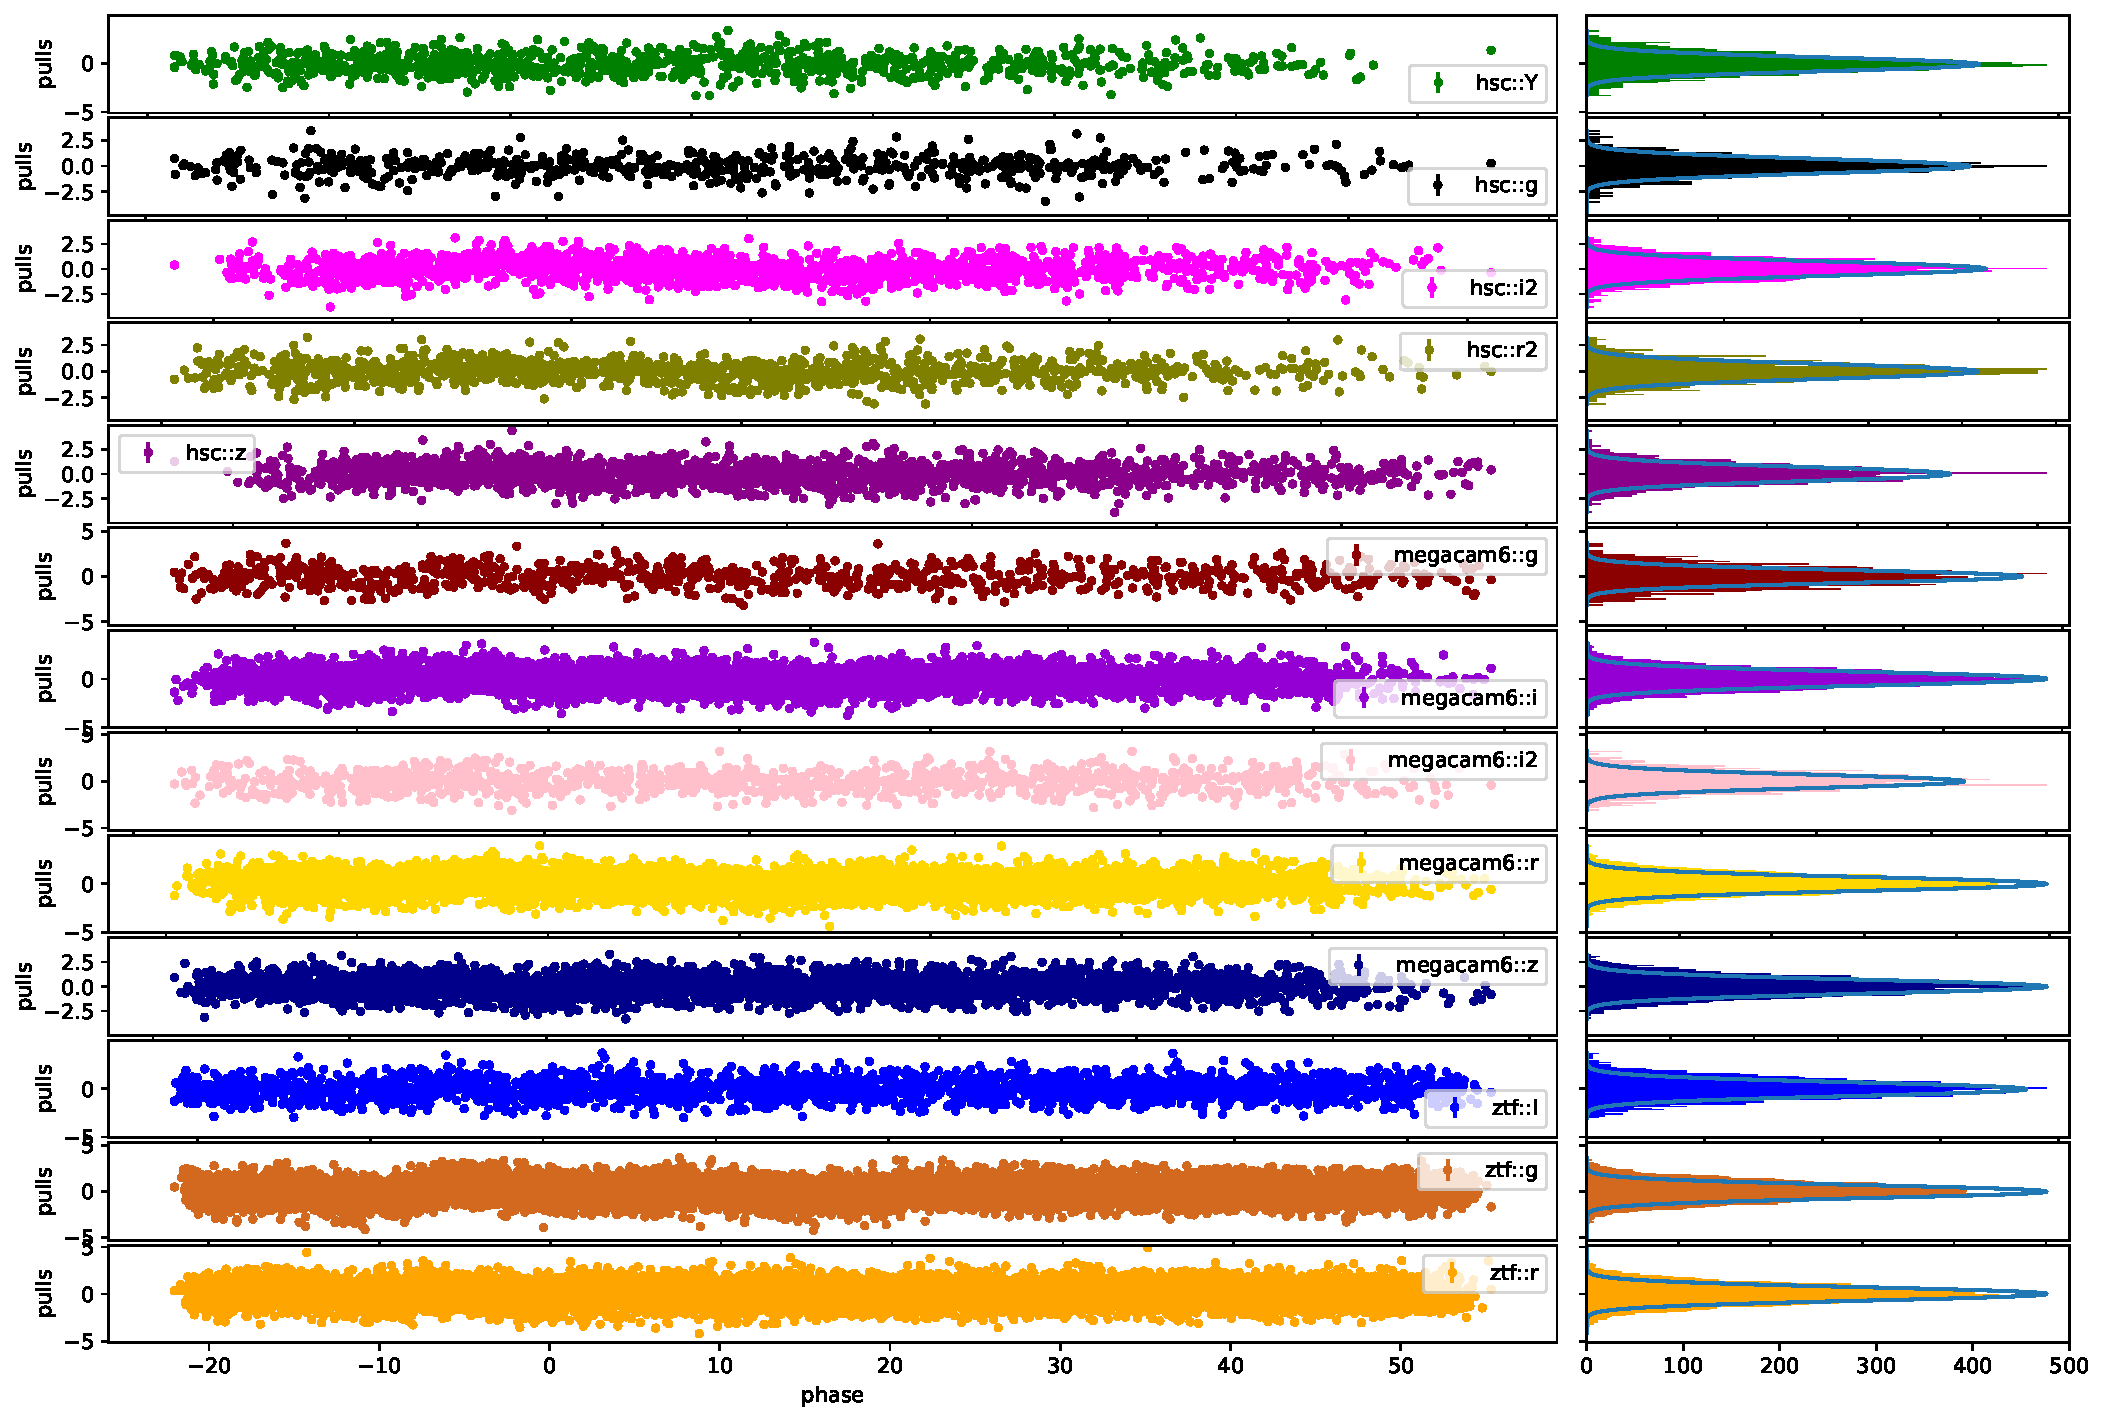
\includegraphics[width=1\textwidth]{MainLayout/DC_chapter/figures/band_resid.pdf}
    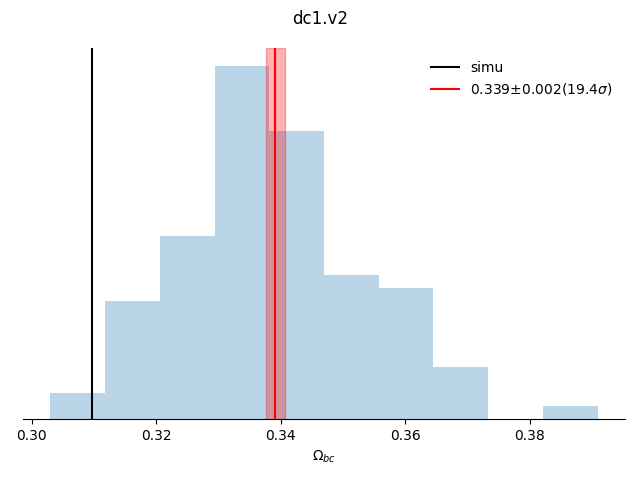
\includegraphics[width=0.6\textwidth]{MainLayout/DC_chapter/figures/new_fig/flcdm.png}
    \caption{Distribution of $\Omega_m$ for a fixed value of $w=-1$. 
    The red line represents the mean value the recovered $\Omega_m$ as well its 
    standard deviation. The black line represents the expected results used as input for the simulation.}
    \label{fig:om_dist}
\end{figure}

\section{Conclusion}

This chapter presented the first application of the NaCl framework
to real data on the SNfactory dataset and 
to simulated \textsc{Lemaître}-like datasets through the pre-DC1 
validation programme. The results demonstrate that NaCl accurately 
describes the spectrophotometric evolution of Type Ia supernovae and 
that its Fisher uncertainty estimates are consistent with the empirical uncertainties for the large majority of parameters, with a small overestimate in the empirical 
uncertainties that is consistent with finite-sample noise. However, 
significant biases were identified in the reconstructed distance 
moduli near the survey transition redshifts $z \approx 0.1$ and 
$z \approx 1$, which likely propagate into the cosmological parameter 
inference as biases in both $\Omega_m$ and $w$. 
The origin 
of these biases has not yet been conclusively identified, with 
possible contributions from residual model artifacts associated with 
the regularization and effective selection effects introduced by the 
quality cuts. 
Resolving these 
biases is the primary objective before the pipeline can be applied to the blinded 
\textsc{Lemaître} dataset. Accurate distance measurements are 
also of significant importance for the $f\sigma_8$ analysis, making this 
validation work directly relevant to both the dark energy and 
growth rate science goals of the \textsc{Lemaître} project.


%\begin{figure}[ht]
%    \centering
    %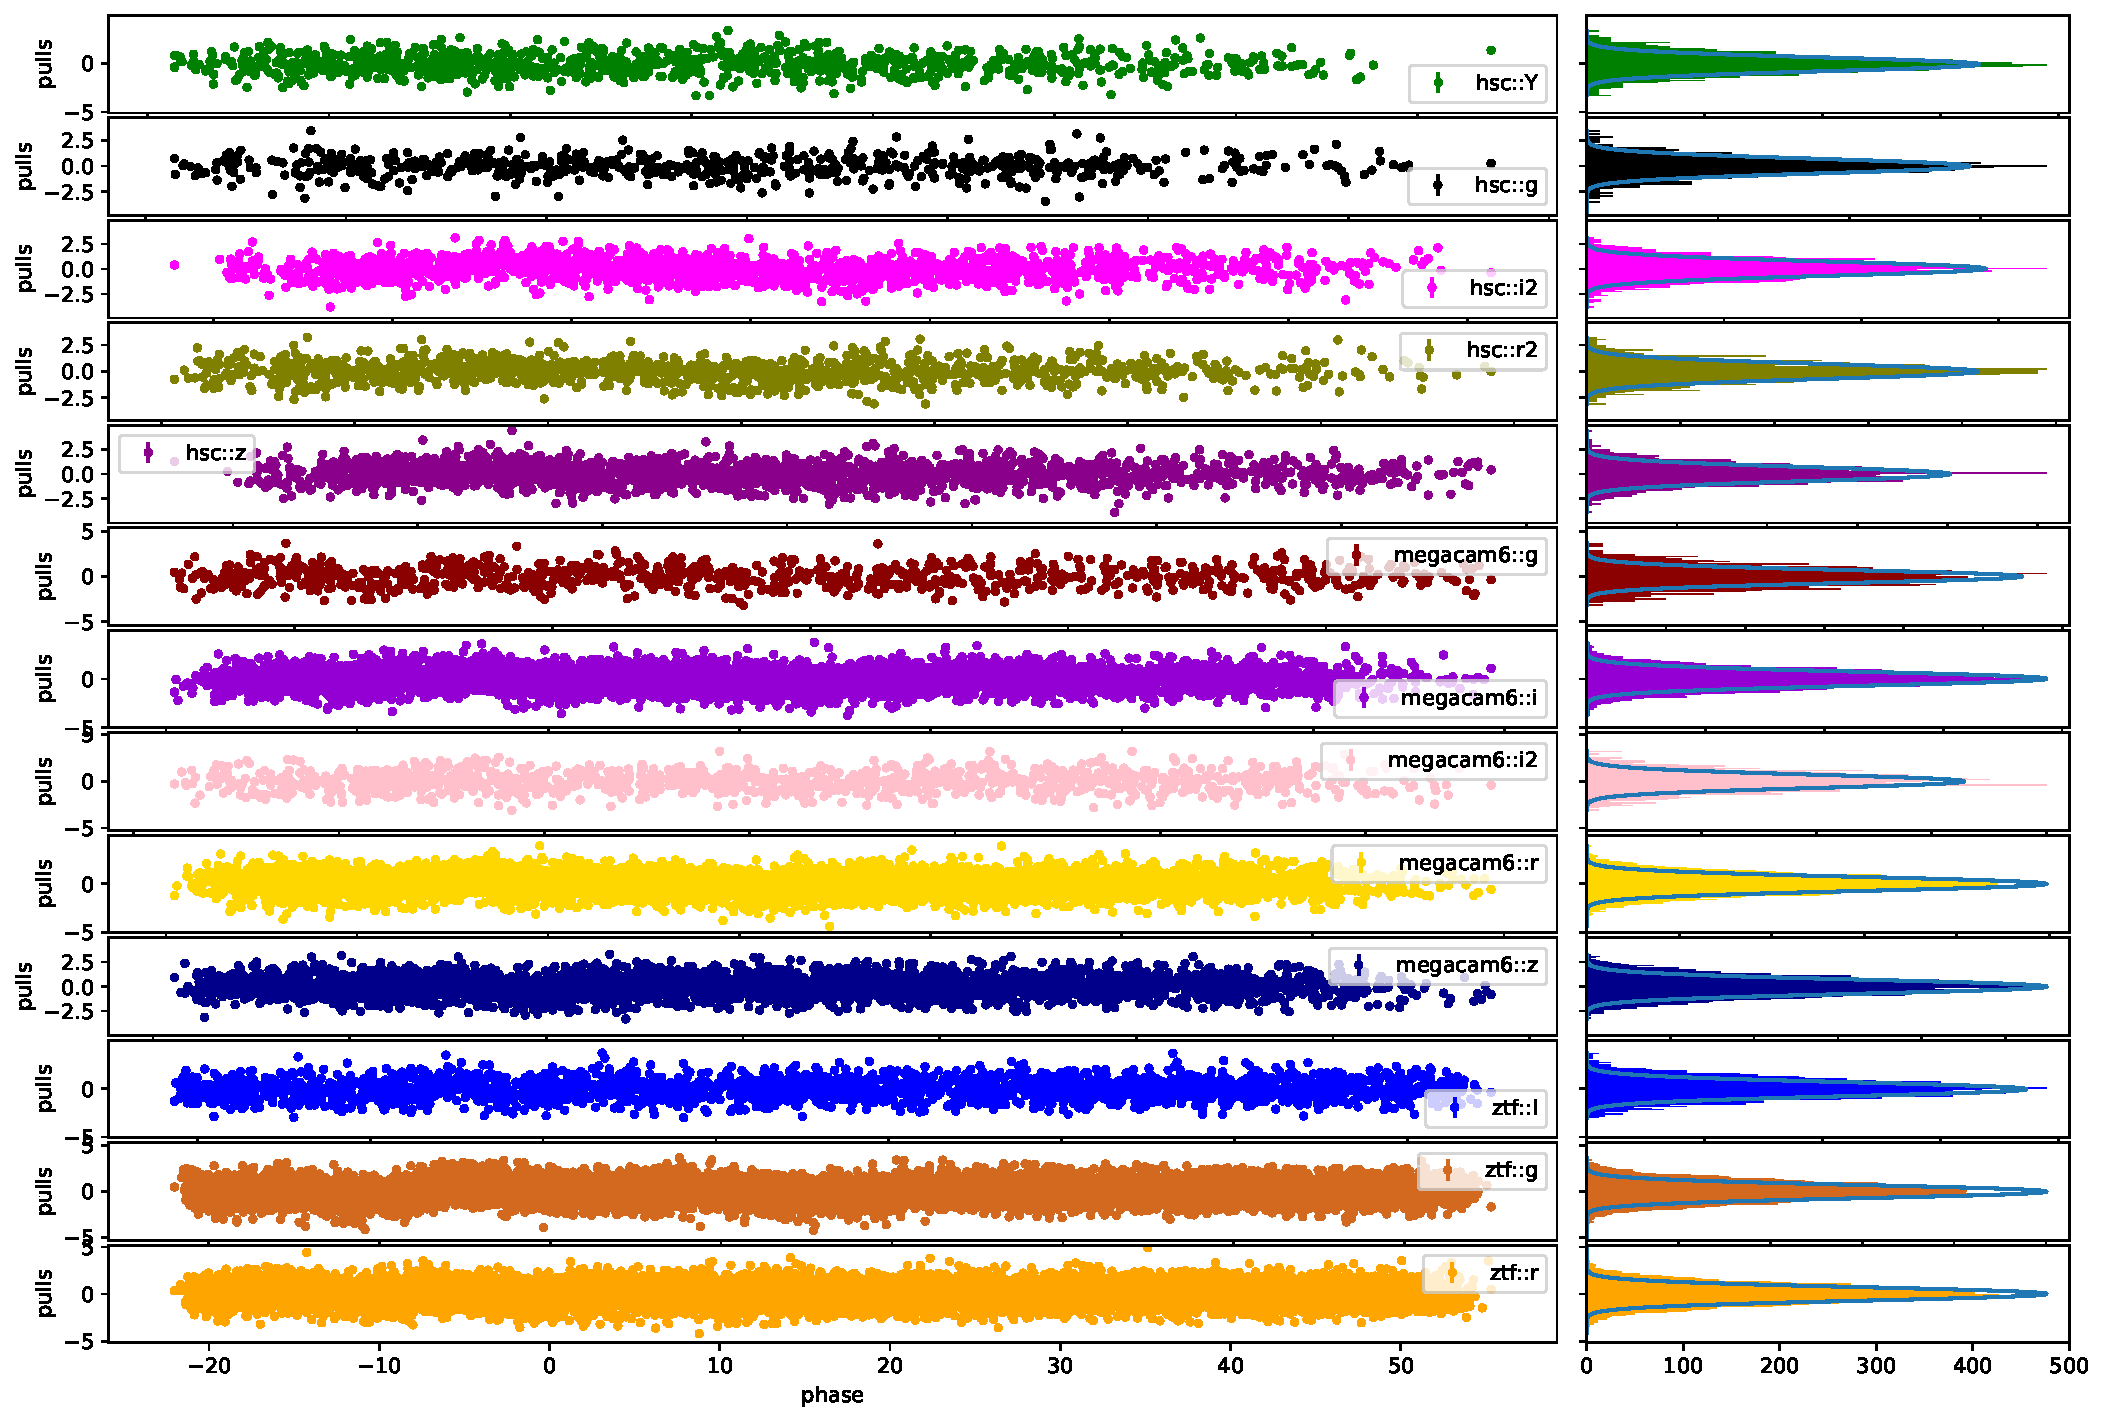
\includegraphics[width=1\textwidth]{MainLayout/DC_chapter/figures/band_resid.pdf}
%    \includegraphics[width=0.8\textwidth]{MainLayout/DC_chapter/figures/None}
%    \caption{$\Omega_m$ and $w$ coverage for 100 realization of pre-DC1}
%    \label{fig:dc1_om_w_coverage}
%\end{figure}




\chapter{Field-level inference for cosmological analyses}\label{chap5}
\minitoc 
\section{Introduction to Field-level Inference}
\subsection{Definition and Motivations}

\subsubsection{Definition}

This definition is mostly taken from \cite{Leclercq_2025}. A field-level inference generally refers to methods and techniques used to infer 
physical fields alongside a set of parameters from observations, without relying on compressed data from the corresponding field. 
A field-level inference belongs to the class of inverse problems, whose objective is to infer the underlying causes of a set of observations by modeling the processes 
that generated them. In our case, we are interested in accessing the initial conditions of the underlying matter density field and velocity field. The goal is 
to extract the maximum amount of information regarding structure formation. 
By modeling the full field instead of relying on compressed summary 
statistics, one can incorporate more complex physical information. However, the inference becomes more sensitive to mismodeling and systematics, and could lead to more biased 
results if not accounted for properly.

\subsubsection{Motivations}

There are a number of motivating factors favoring the use of field-level inference rather than summary statistics when it comes to the study of structure formation. 
Unlike compressed statistics such as the matter power spectrum ($ \propto \left \langle \delta(\mathbf{k_1})  \delta(\mathbf{k_2})\right \rangle$), a field-level inference preserves all statistical 
information such as higher-order correlations \cite{Leclercq_2021}. The structures 
observed today are non-linear and non-Gaussian, meaning correlations of higher order such as the bispectrum ($ \propto \left \langle \delta(\mathbf{k_1})  \delta(\mathbf{k_2}) \delta(\mathbf{k_3})\right \rangle$) 
or trispectrum ($ \propto \left \langle \delta(\mathbf{k_1})  \delta(\mathbf{k_2}) \delta(\mathbf{k_3}) \delta(\mathbf{k_4})\right \rangle$) are non-zero and therefore contain additional 
information on cosmological parameters. Since the field-level inference aims at reconstructing the entire underlying field as well as its structures, these correlations will always 
be accounted for at all orders. Moreover it preserves phase information. The compressed statistics mainly calculate the amplitudes of the correlations that exist while missing out 
on the phase for which these amplitudes are possible. 
For example, the contribution of two overdense regions to the correlation function depends only on their separation and not on their absolute positions. 
Consequently, relocating the pair elsewhere in the Universe while preserving their separation would leave their contribution unchanged.

\noindent Another motivation for field-level inference is reducing the uncertainties that arise due to cosmic variance of the local-Universe. Traditional summary statistics assume ergodicity 
i.e. averaged measurements over a sufficiently large volume of the Universe approximate the averages over many hypothetical realizations, which becomes problematic in 
the local Universe due to the limited volume. With field-level inference, the goal is to reconstruct the specific realization that produces our observations, allowing us to 
properly adjust our model parameters to that realization (e.g. \cite{Porqueres_2021, Ramanah_2019}). 
The outcome of a field-level inference on observations of our Universe is what we call a Digital Twin, a cosmic variance-aligned numerical simulation of the dark matter 
density field that should, in theory, match the density field of our observable Universe. \\


\subsubsection{Performing a Field-level Inference}

Unlike the frequentist maximum likelihood approach adopted in the NaCl spectrophotometric framework, field-level inference is better suited using a Bayesian 
statistical framework. In the frequentist approach, parameters are treated as fixed unknowns and inferred by maximizing the likelihood 
$\mathcal{L}(d|\theta)$, where $d$ is the observed data and $\theta$ are a set of parameters, 
with uncertainties estimated from Fisher information matrix. This is well suited for NaCl as the number of parameters can be handled by a single personal computer. 
However, field-level inference involves a parameter space of order $N^3$ for an $N^3$ voxel 
grid. In our case $N$ can go from $64$ to $256$, giving us $10^5 - 10^7$ initial condition parameters alongside the model parameters (\cite{Jasche_2019,Mcalpine_2025}). 
Although maximum likelihood estimation can still be performed in such a high-dimensional space using gradient-based methods, 
efficiently exploring the full posterior distribution becomes considerably more challenging. 


The Bayesian framework addresses this by treating both data and parameters 
as random variables. The central equation comes from Bayes' theorem which states that the probability that an event $A$ occurs knowing an event $B$ has occurred is written as:
\begin{equation}
    \mathcal{P}(A|B) = \frac{\mathcal{P}(B|A) \cdot \mathcal{P}(A)}{\mathcal{P}(B)} = \frac{\mathcal{P}(A \cap  B)}{\mathcal{P}(B)}
\end{equation}
For a field-level inference, we are attempting to determine the initial conditions $\delta^{IC}$ and a set of model parameters $\theta$ given a set of observations $d$.
Ideally, we would like to determine the model of the Universe $M$ such as $\Lambda$CDM but this is not currently accessible and will be 
assumed as constant in our analysis (Section \ref{sec:BORG}).We nevertheless retain $M$ in the following expressions to illustrate 
the most general form of the posterior, but omit it in subsequent sections where the model is fixed. Thanks to Bayes' theorem, we get: 
\begin{equation}
    \mathcal{P}(\delta^{IC}, \theta, M | d) = \frac{\mathcal{P}(d | \delta^{IC}, \theta, M) \cdot \mathcal{P}(\delta^{IC}, \theta, M)}{\mathcal{P}(d)}
\end{equation}
The term $\mathcal{P}(d)$ is a constant with respect to the rest of the parameters so we will omit it for simplicity. 
Using the chain rule decomposition $\mathcal{P}(A, B|C) = \mathcal{P}(A|C) \cdot \mathcal{P}(B|A, C)  $, we can rewrite the full posterior as:
\begin{equation}
    \mathcal{P}(\delta^{IC}, \theta, M | d) = \mathcal{P}(M | d) \cdot \mathcal{P}(\delta^{IC}, \theta | d, M)
\end{equation}
\begin{equation}
    \mathcal{P}(\delta^{IC}, \theta, M | d) = \mathcal{P}(M | d) \cdot \mathcal{P}(\theta | d, M) \cdot \mathcal{P}(\delta^{IC} | d, M, \theta)
    \label{eqn:bayesian_borg}
\end{equation}
We can see three distinct terms:
\begin{itemize}
    \item The term $\mathcal{P}(M | d)$ describes which cosmological model fits the data best ($\Lambda$CDM or $w$CDM, GR or modified gravity, etc...). 
    \item The term $\mathcal{P}(\theta | d, M)$ estimates the model parameters given the data and a cosmological model ($\Omega_m$, $\sigma_8$, bias model parameters, etc...).
    \item The term $\mathcal{P}(\delta^{IC} | d, M, \theta)$ estimates the initial conditions for a specific realization of the Universe, given the data, a model and its parameters.
\end{itemize}
The posterior naturally distinguishes between regions of 
the density field that are well constrained by the data and those that are not, where the posterior defaults to a prior specified beforehand. The nuisance parameters 
can be marginalized, integrated over their full posterior distribution, which correctly propagates all their uncertainty into the parameters of interest, unlike 
in the frequentist approach which explores only a restricted region of the full parameter space. \\

The inherent high dimensionality of these analyses requires advanced statistical techniques. First, a differentiable forward model is generally employed to describe the 
evolution of the initial matter field and enable the use of gradient-based sampling methods. Second, the inference algorithm must be computationally efficient to make 
the exploration of the high-dimensional parameter space tractable. 

\subsection{Field-level Inference Pipeline}

\subsubsection{The BORG Framework}

This PhD work uses the \textit{Bayesian Origin Reconstruction from Galaxies} (BORG) (\cite{Jens_2013, Jasche_2019}), a field-level forward model framework designed to 
reconstruct the initial conditions of the Universe given a set of observations. 


The BORG framework is illustrated in Figure \ref{fig:BORG_schematic} and is composed of three main ingredients. First, 
the forward model generates Gaussian initial conditions on a grid of $N^3$ voxels, models the nonlinear 
evolution with a gravity model and connects the nonlinear matter density field to the 
observable of interest. Second, the data likelihood has an explicit functional form that depends on 
the observable of interest, for instance for application to galaxy surveys, we may use a Poisson 
likelihood for galaxy counts. The third component is the parameter sampler that needs to be 
efficient enough in order to sample the very high dimensional parameter space. Moreover, BORG 
employs a modular parameter sampler design that allows any additional parameters introduced 
by a model component to be included through a Gibbs sampling scheme. 
The BORG algorithm will be described in more detail in Section \ref{sec:BORG}. 
Applications of BORG to simulated and real data will be discussed in Section \ref{sec:applications_fli}. 

\begin{figure}[ht]
    \centering
    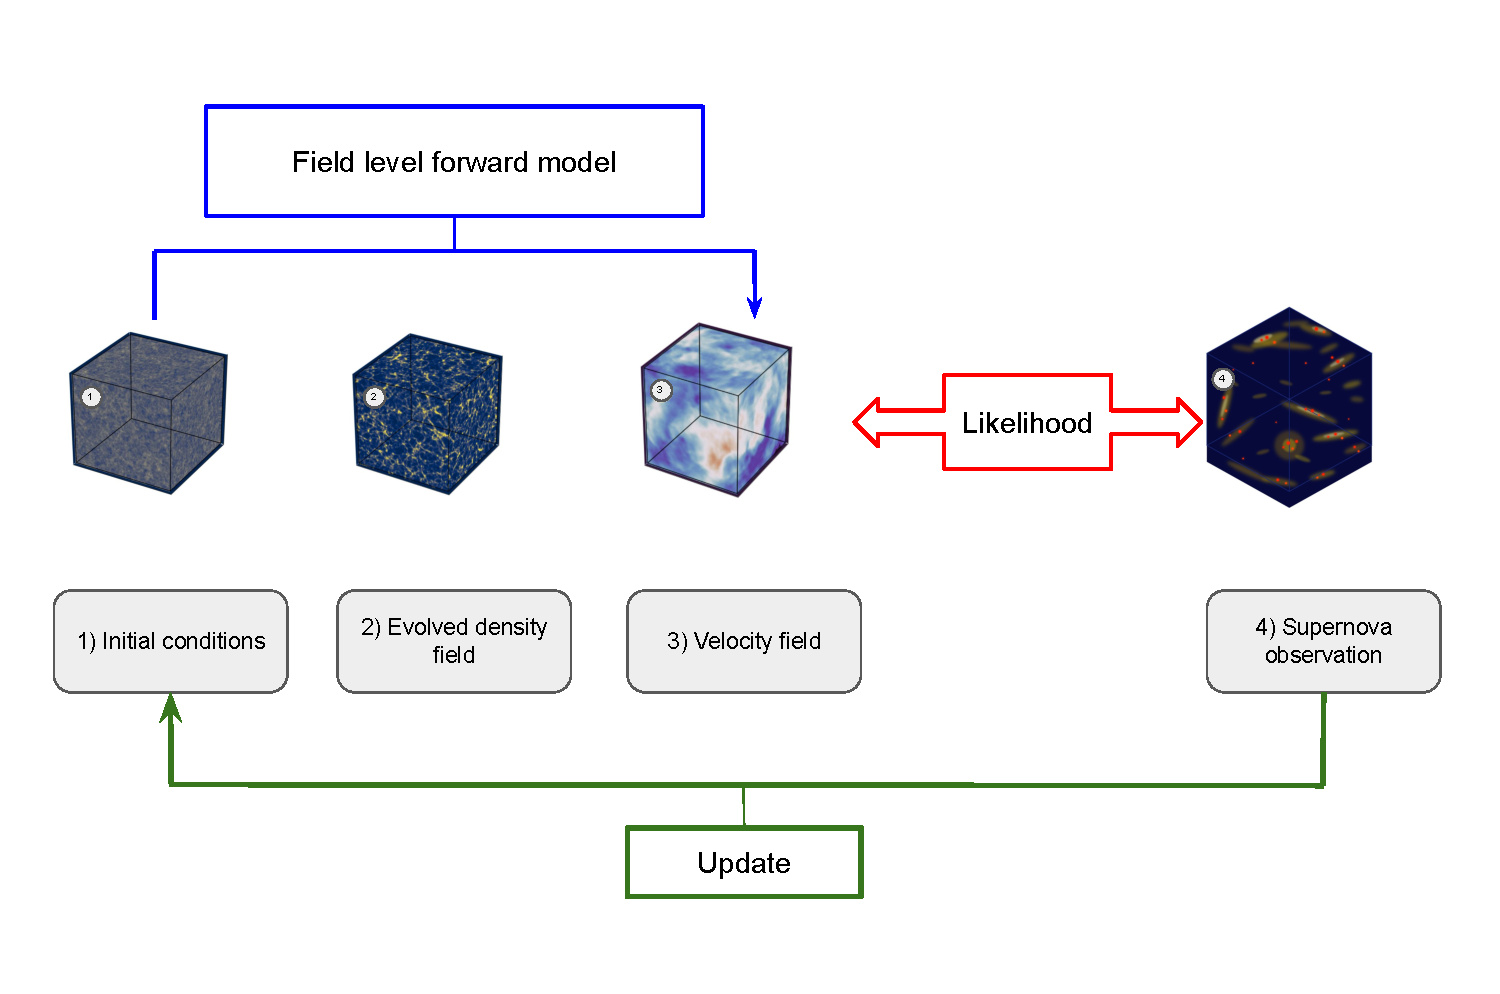
\includegraphics[width=1.0\textwidth]{MainLayout/BORG_chapter/figures/BORG_sn_schematic.pdf}
    \caption{Schematic summarizing what BORG intends to do when faced with Type Ia supernova data. First we start with a set of initial conditions. The initial conditions 
    then evolve using a gravity solver to obtain the density field today. Observational effects are applied to match the observations, such as selection effects and 
    survey footprint. Finally we evaluate a likelihood. The goal is to adjust the initial conditions and the model parameters to maximize the likelihood. Adapted from \url{https://indico.ijclab.in2p3.fr/event/8881/contributions/28072/attachments/20421/28316/COPHY_Lavaux.pdf}.}
    \label{fig:BORG_schematic}
\end{figure}

\subsubsection{Other Approaches}

As described in the previous section, BORG is arguably the most advanced end-to-end field-level inference 
pipeline. Other approaches have been developed, in this section we will describe two of them. 

The first one is 
the FlowPM model (\cite{Modi_2020}), a differentiable cosmological N-body simulator using the Particle Mesh (PM) gravity solver (more details in Section \ref{sec:gravity_model}) 
designed to run on GPU for accelerated results using a neural network framework. It was shown to be able to reconstruct 
cosmological fields when implemented in a forward model Bayesian framework. This model was tested only on simulations. 

The second model was developed by \cite{Simon_2025} based on the JaxPM\footnote{\url{https://github.com/DifferentiableUniverseInitiative/JaxPM}} 
gravity solver, an N-body simulator using PM coded in Python-Jax and can run on GPU. The model was tested using different samplers and they highlight the importance of carefully preconditioning 
latent variables in the model in order to achieve unbiased results on simulations. It also highlighted the differences between the samplers and the different algorithms that can be used to 
sample the likelihood. 

More recently, works by \cite{Bayer_2026} demonstrated the capabilities of running a field-level inference when trying to reconstruct the BAO signal 
in comparison to traditional methods where a hybrid Effective Field Theory approach was applied instead of a PM gravity solver. The results have shown an improvement in the 
BAO signal reconstruction using field-level inference in comparison to standard methods. \\


\subsection{Applications of Field-level Inference in Cosmology} \label{sec:applications_fli}

\subsubsection{Galaxy Clustering}

Examples of direct applications on real galaxy clustering data are the Manticore products obtained with the BORG forward model (\cite{Jens_2013, Jasche_2019}). Manticore-Local (\cite{Mcalpine_2025}) is a set of reconstructed dark matter simulations to 
match the observations in the 2M++ galaxy catalogue (\cite{Lavaux_2011}) with galaxies up to a redshift of $z \lesssim 0.1$. Manticore-Deep (\cite{Mcalpine_2026}) extends the work done on Manticore-Local 
by applying the algorithm on five galaxy catalogues 2M++, 6dFGS, 2dFGRS, SDSS, and BOSS (\cite{Lavaux_2011,Jones_2009_6dFGS,Colless_2003_2dFGRS,
York_2000_SDSS,Dawson_2013_BOSS}) reaching a redshift of $z \lesssim 0.7$, the largest Digital Twin that exists to date at a resolution of $\sim 4 \, h^{-1}.\text{Mpc}$. 
This gives us access to more than just cosmological parameters but a better understanding of the local 
structures in the Universe by being able to observe them one by one like the Virgo cluster or the Great Attractor. 
It also allows us to access hard-to-observe properties such as the velocity field, formation histories and tidal fields. 
It can also be used to further the study of void catalogues 
which are sensitive probes of the dark matter fields as it was done in \cite{Malandrino_2026}. \\


There is also the work of \cite{Nguyen_2024} on the study of galaxy clustering at the field level on simulations. 
The paper focuses primarily on the constraints obtained on the $\sigma_8$ 
parameter. Two methods were used to constrain the parameter on two N-body dark matter mocks' halos. 
The first method uses a differentiable forward model that incorporates a non linear gravity 
solver LEFTfield (\cite{Schmidt_2021}) that combines Effective Field Theory and Lagrangian Perturbation Theory (see Section \ref{sec:gravity_model}) and 
evolves the initial conditions 
to match the simulated halos. The use of the fully evolved field gives direct access to the cosmological parameters. The second method extracts the cosmological 
parameters from 
the power spectrum and bispectrum of the mocks ($P+B$ method). The results obtained show improvements on the $\sigma_8$ constraints with the field-level inference 
with a factor of 1.9 to 5.2 
based on the limiting modes included in the analysis ($k_{\text{max}} = 0.10 h \text{Mpc}^{-1}$ and $k_{\text{max}} = 0.12 h \text{Mpc}^{-1}$ respectively)
and the mock used. Figure \ref{fig:nguyen} shows the constraints obtained from methods on one of the mocks. \\ 

\begin{figure}[ht]
    \centering
    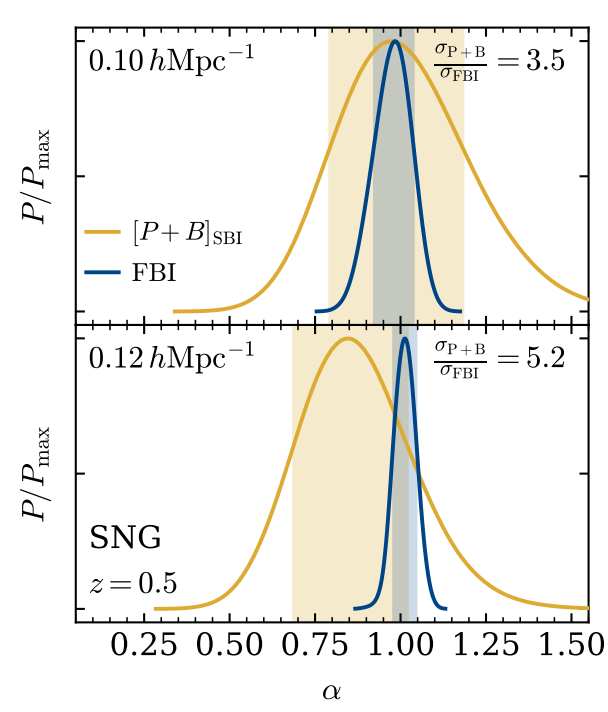
\includegraphics[width=0.6\textwidth]{MainLayout/BORG_chapter/figures/nguyen.png}
    \caption{Posterior distribution of the reconstructed value of $\sigma_8 /\sigma_{8, \text{true}} $. In blue are the results from the field-level inference and 
    in yellow are the results from the $P+B$ method. The top Figure is for a limiting mode of $k_{\text{max}} = 0.10 h \text{Mpc}^{-1}$ and the bottom for 
    $k_{\text{max}} = 0.12 h \text{Mpc}^{-1}$. Taken from \cite{Nguyen_2024}.}
    \label{fig:nguyen}
\end{figure}


\subsubsection{Weak Lensing}

The following study highlights the constraining power of field-level inference. It was done by \cite{Porqueres_2023, Porqueres_2021} on simulated weak lensing catalogues. 
The study was conducted using the 
BORG framework. The developed hierarchical forward model included astrophysical systematics of intrinsic alignment and baryon feedback in addition to the gravity 
solver. The resulting model has been called BORG-WL. The model was tested on self-consistent simulations and was used to constrain both the matter content $\Omega_m$ and 
$\sigma_8$. This was then compared to the traditional summary statistics by inferring the parameters using the angular power spectrum. They obtain the following results in 
Figure \ref{fig:porqueres}. The results show much tighter constraints on both parameters as well as being able to break the degeneracy between them. However, 
there is no uncertainty associated with photometric redshift or shape measurement that were accounted for in this work. \\

\begin{figure}[ht]
    \centering
    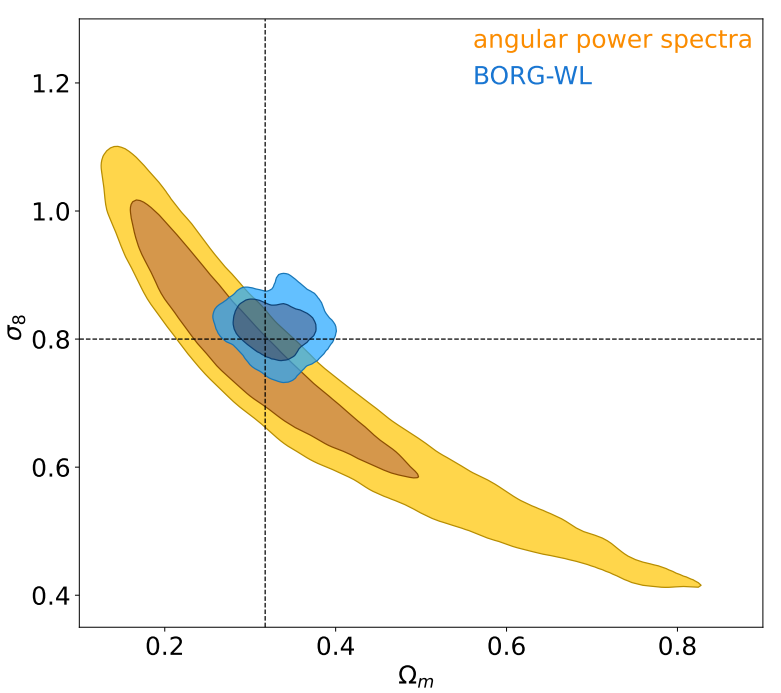
\includegraphics[width=0.6\textwidth]{MainLayout/BORG_chapter/figures/porqueres.png}
    \caption{Comparison of $\Omega_m$-$\sigma_8$ constraints from BORG-WL (blue) and the angular power spectrum (yellow) for self-consistent mocks. Taken from \cite{Porqueres_2023}.}
    \label{fig:porqueres}
\end{figure}


\subsubsection{Primordial non-Gaussianities}

Primordial non-Gaussianities (PNGs) are small deviations from the Gaussian statistics of the primordial density perturbations. 
Their detection would provide valuable insight into the physics of inflation, as different inflationary scenarios predict distinct non-Gaussian signatures (\cite{Chen_2010}). 
An application of field-level inference to this problem was first presented by \cite{Andrews_2023}, where the BORG framework was extended to 
jointly infer the initial conditions and the local primordial non-Gaussianity parameter $f_{\text{NL}}$. 
Applied to SDSS-III/BOSS-like mock galaxy catalogues, the method achieved a factor of $\sim2.5$ improvement over the observational constraints available at the time.

More recently, \cite{Andrews_2026} extended this framework to realistic halo catalogues generated from the Quijote N-body simulations (\cite{Villaescusa_2020}). 
Compared to a joint power spectrum and bispectrum analysis, the field-level approach achieved a factor of $\sim1.3$ improvement in the 
uncertainty on $f_{\text{NL}}$. The inference was also tested on multiple gravity solvers to assess the impact of resolving small-scales on the measurement of $f_{\text{NL}}$.


\subsubsection{Peculiar Velocities}


We present several studies that assess the performance of field-level inference for reconstructing the cosmic velocity field. 
A widely used approach for reconstructing the local velocity field is the linear reconstruction method of \cite{Carrick_2015}, 
which uses the luminosity-weighted galaxy density field from the 2M++ survey \cite{Lavaux_2011}. 
While such linear reconstructions provide an effective description of the large-scale velocity field, they do not fully capture the non-linear gravitational 
evolution of structure on smaller scales. 
Recent comparisons of local Universe reconstructions have demonstrated the importance of 
accounting for these non-linearities when reconstructing the velocity field \cite{Stiskalek_2025_b}. 


We first consider the work of \cite{Boruah_2020}, which reconstructed the large-scale velocity field from the 2M++ galaxy survey \cite{Lavaux_2011} using the linear 
reconstruction method of \cite{Carrick_2015}. The reconstructed velocity field was subsequently compared with independent peculiar velocity measurements 
from Type Ia supernovae and Tully-Fisher catalogues, allowing for a measurement of $f\sigma_8$. 
However, subsequent work has shown that the inferred $f\sigma_8$ is sensitive to calibration effects and to the cosmic variance associated 
with the finite survey volume (\cite{Hollinger_2024}). 
The field-level approach adopted in this work instead incorporates the peculiar velocity tracers directly into the inference of the underlying density and velocity fields. 
This provides a unified framework in which the information from the tracers, together with the measurement uncertainties and the 
uncertainties associated with the reconstructed fields, is propagated jointly through the inference. 
Rather than using the peculiar velocity measurements only to assess an independently reconstructed velocity field, they directly contribute to constraining the field itself. \\


The second study, by \cite{Prideaux_Ghee_2022}, extended the BORG framework to reconstruct the initial matter density and velocity fields directly from peculiar velocity tracers 
using Lagrangian Perturbation Theory (LPT). 
The method was validated using mock catalogues extracted from \texttt{GADGET2} N-body simulations (\cite{Springel_2005}). 
Their results demonstrated that accurate velocity field reconstructions can be achieved by incorporating peculiar velocity tracers directly into a Bayesian field-level 
inference, even when using an approximate gravitational forward model. 
In particular, the use of Lagrangian perturbation theory allowed the reconstruction to extend into the mildly non-linear regime, as illustrated in Figure \ref{fig:james_vel}.
This motivates the use of non-linear 
gravity solvers when attempting to reconstruct the velocity field from 
peculiar velocity tracers.  
However, the implementation remains a proof of concept. 
The authors identify the use of more accurate non-linear gravity and velocity models as an important direction for future work. 
Furthermore, their validation is performed using mock tracers, with some 
simplifying assumptions regarding the observed distances. 
Applications to real data would therefore require accounting for the fact 
that the observed distance modulus provides an estimate of the true distance, 
and propagating the associated uncertainty through the field-level inference. \\

\begin{figure}[ht]
    \centering
    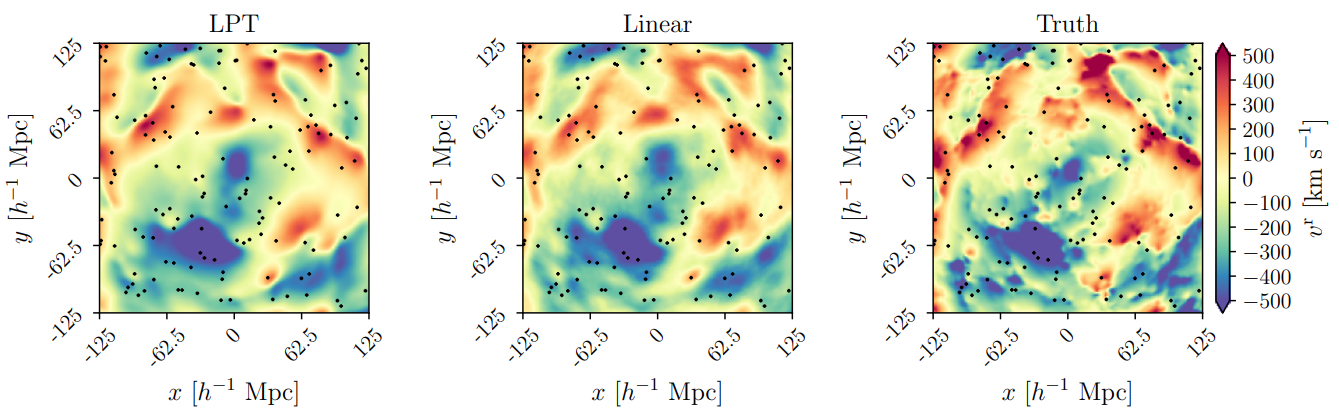
\includegraphics[width=0.9\textwidth]{MainLayout/BORG_chapter/figures/james_vel.png}
    \caption{Comparison of reconstructed velocity fields from \cite{Prideaux_Ghee_2022}. \textit{Left:} reconstruction using Lagrangian Perturbation Theory (LPT), 
    which captures mildly non-linear gravitational evolution. \textit{Center:} reconstruction using linear perturbation theory. \textit{Right:} reference velocity 
    field from the \texttt{GADGET2} N-body simulation.}
    \label{fig:james_vel}
\end{figure}



Lastly, we present the study conducted by \cite{Stiskalek_2025_b} on the reconstruction of velocity fields. The paper compares different methods in reconstructing the velocity field 
from a reconstruction of the local Universe to peculiar velocity catalogues from direct distance tracers.  
Each reconstruction can be used to infer the velocity field. We will list the different local Universe reconstruction methods 
in Table \ref{tab:velocity_olympics} and show the results from the different methods in Figure \ref{fig:olympics_dens}, which highlights how accounting for non-linearities in the 
gravity model translates onto the small scales of the density fields. 
It is important to note that amongst those methods, 
the CSiBORG1 and CSiBORG2 reconstructions are field-level inferences with BORG.  

\begin{table}[ht]
    \centering
    \caption{Different local Universe reconstruction methods.}
    \label{tab:velocity_olympics}
    \begin{tabularx}{\textwidth}{|l|c|X|c|}
    \hline
    Model & Alias & Description & Resolution \\
    \hline
    \cite{Carrick_2015}
    & C15
    & Linear inverse modelling using a luminosity-weighted galaxy density field. Used the 2M++ galaxy catalogue \cite{Lavaux_2011}. & $4\,h^{-1}\,\text{Mpc}$. \\
    \hline
    \cite{Lilow_2024}
    & L24
    & Machine-learning inverse method trained on Quijote simulations. Used the 2MRS galaxy catalogue \cite{Huchra_2012}. & $3.1\,h^{-1}\,\text{Mpc}$. \\
    \hline
    \cite{Jasche_2019}
    & CSiBORG1
    & BORG forward model. Used the 2M++ galaxy catalogue. & $2.6\,h^{-1}\,\text{Mpc}$. \\
    \hline
    \cite{Stopyra_2023}
    & CSiBORG2
    & BORG forward model with an improved gravity solver. Used the 2M++ galaxy catalogue. & $2.6\,h^{-1}\,\text{Mpc}$. \\
    \hline
    \cite{Sorce_2018, Sorce_2020}
    & S18
    & Constrained realization using a Wiener filter, which combines the peculiar velocity measurements with prior statistical information, and the reverse Zel'dovich approximation. Used CosmicFlows-2 peculiar velocities \cite{Tully_2013}. & $1.9\,h^{-1}\,\text{Mpc}$. \\
    \hline
    \cite{Courtois_2023}
    & C23
    & HMC sampling of the density field at $z=0$ constrained by peculiar velocities. Used CosmicFlows-4 peculiar velocities \cite{Tully_2023}. & $3.9\,h^{-1}\,\text{Mpc}$. \\
    \hline
    \end{tabularx}
    \end{table}


\begin{figure}[ht]
    \centering
    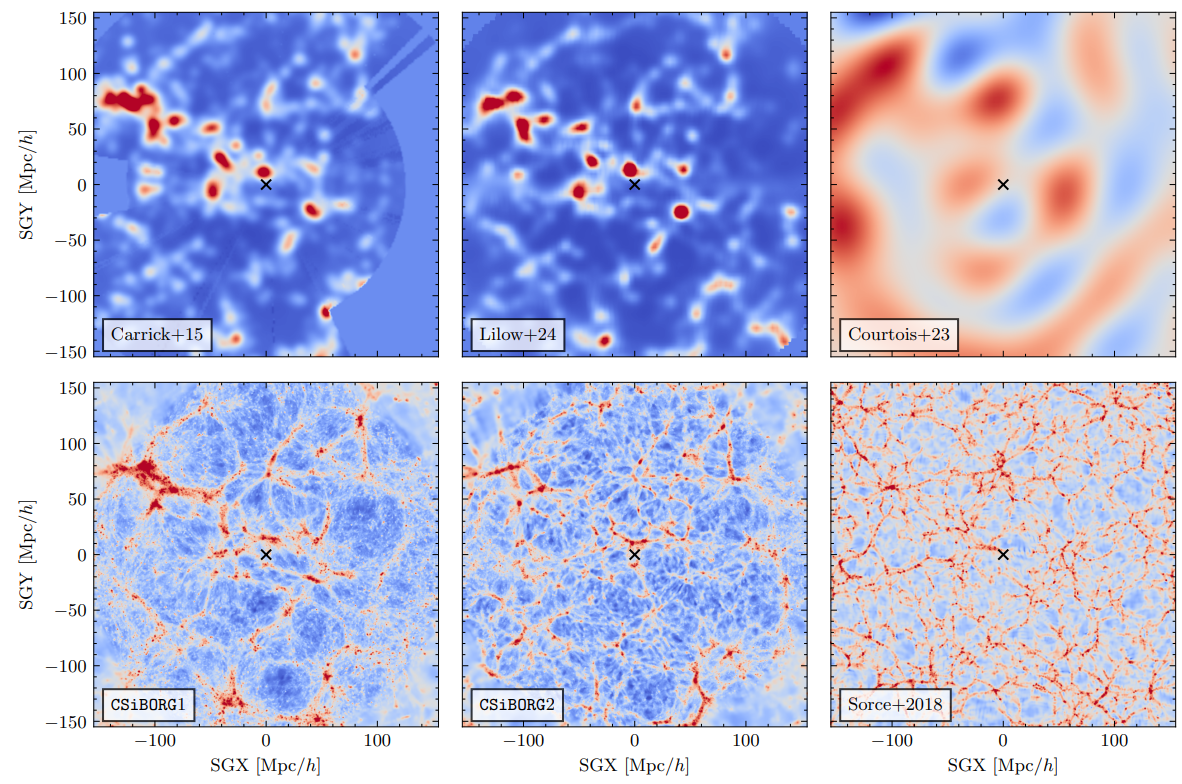
\includegraphics[width=0.9\textwidth]{MainLayout/BORG_chapter/figures/olympics_dens.png}
    \caption{Slice of the reconstructed matter field from each method used and described in Table \ref{tab:velocity_olympics}. The slices were chosen to look at the same portion 
    of the sky.}
    \label{fig:olympics_dens}
\end{figure}

The velocity fields are then compared to peculiar velocities from Tully-Fisher and one from Type Ia supernova catalogues. 
There are multiple metrics used to assess how accurate the velocity field reconstructions are, mainly relying on computing the evidence $\mathcal{Z}$ , i.e the probability of observing the 
peculiar velocities given a model. This is presented in Figure \ref{fig:olympics_rank} where we can see that the BORG reconstruction outperforms the other models. This highlights the importance 
of accounting for non-linearities when it comes to assessing velocity fields. 
The better performance of the BORG reconstructions 
therefore demonstrates the importance of modeling non-linear gravitational 
evolution when predicting the velocity field on the scales probed by peculiar 
velocity tracers. This motivates moving beyond traditional linear velocity 
reconstructions and incorporating non-linear structure formation directly 
within the inference. \\

In this work, we adopt such a field-level approach using the BORG framework, 
where the peculiar velocity tracers directly constrain the underlying density 
and velocity fields through a non-linear forward model. In the next section we will describe the core of the BORG framework. 

\begin{figure}[ht]
    \centering
    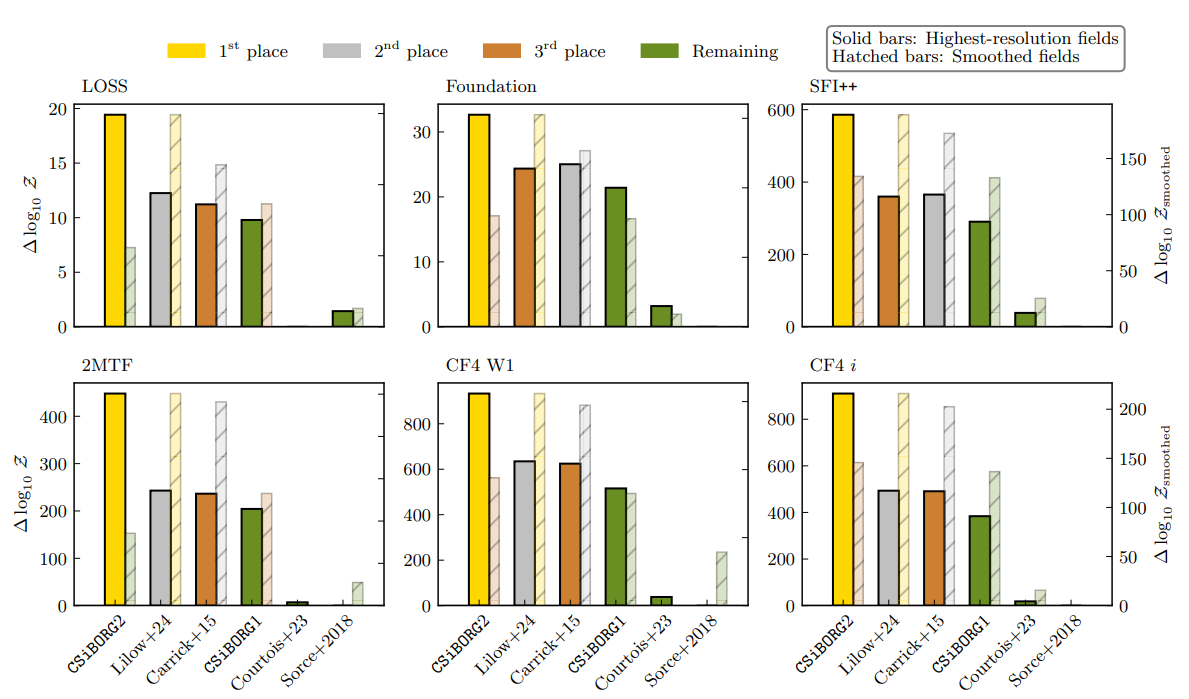
\includegraphics[width=0.9\textwidth]{MainLayout/BORG_chapter/figures/olympics_rank.png}
    \caption{Logarithmic evidence for each method highlighting in gold the most accurate reconstruction then silver, bronze and green in that order. The evidence was calculated 
    for six peculiar velocity catalogues. The LOSS and Foundation catalogues are supernova catalogues while the remaining ones are Tully-Fisher catalogues. Taken from \cite{Stiskalek_2025_b}.}
    \label{fig:olympics_rank}
\end{figure}

\section{Self-consistent simulation analysis}

 - Simulation description
 - Different flavours and tests 
 - Results

\section{ZTF peculiar velocity data challenge (DC PV)}
 - Simulation description and volume limited sample




\chapter{BORG applications on ZTF simulations}\label{chap6}
\minitoc 
We presented in the previous chapter the motivations and potential outcomes of conducting a field inference as well as the BORG algorithm. BORG has proven to be very successful 
when applied to galaxy catalogues as well as show great potential regarding weak lensing. Our goal is advance its applications to type Ia supernovae to eventually run it on the 
ZTF data. We will be presenting in this chapter the steps taken in order to achieve the latter. We will start by presenting the ZTF-Uchuu simulations. 
Then the implementation of a an improved supernova-specific likelihood in BORG. 
Then we will present its results on self-consistent simulations. Finally its application to ZTF-like simulations. \\

\section{ZTF-Uchuu mocks}

The ZTF simulations designed to test the impact of ZTF-supernovae peculiar velocities in a cosmological analysis is called DC PV (Data Challenge 
Peculiar Velocity). These are generated within the ZTF collaboration mainly to test methods in inferring $f\sigma_8$. 
The DC PV simulations are done similarly to the DC simulations as 
described in Chapter 4 with the main differences lie in adding structure information to the simulations. For that, the supernovae are simulated with the help of the Uchuu N-body simulation 
(\cite{Ishiyama_2021}), a high fidelity N-body dark matter simulation in a $2^3 \text{Gpc}.h^{-1}$ box with 2.1 trillion particles which can be seen in Figure \ref{fig:uchuu_nbody} \footnote{N-body and hydrodynamical simulations 
are considered the highest fidelity simulations we can get to describe structure formation as they solving the equations of motion for each particle/fluid without any 
approximations or grid mesh}. The full box is then subdivided into 27 subboxes where the supernovae are simulated up to a redshift of $z=0.11$, giving 27 quasi-independent 
realizations of the DC PV. Each supernova must be simulated where a particle is and is assigned the particle's velocity. This allows us to add proper motion to supernovae 
that is driven by structure formation.\\

\begin{figure}[ht]
    \centering
    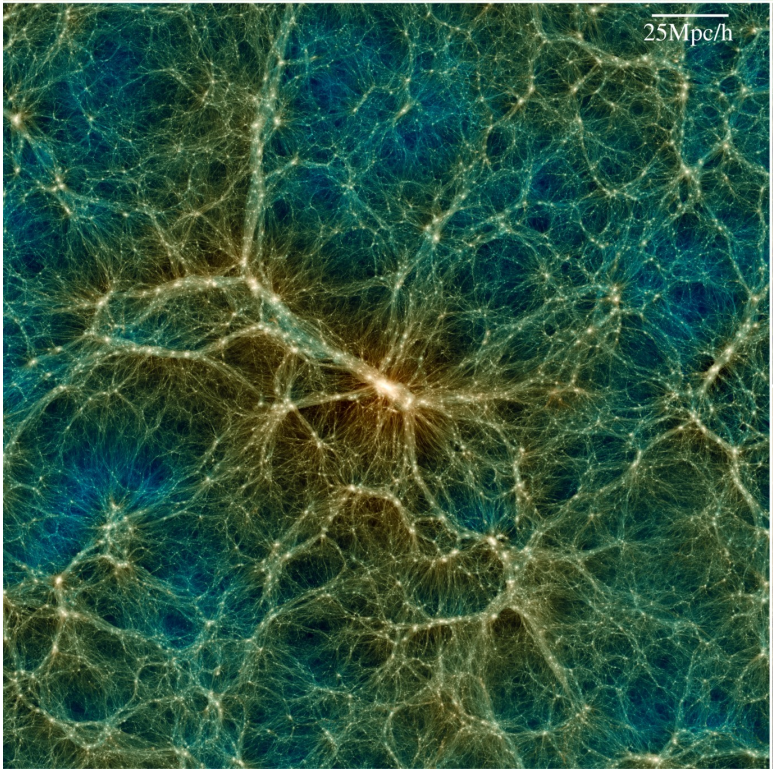
\includegraphics[width=0.7\textwidth]{MainLayout/BORG_chapter/figures/uchuu_nbody.png}
    \caption{Slice taken from the Uchuu simulation covering a box of 250 $\text{Mpc}.h^{-1}$ where each point represents a particle. Taken from \cite{Ishiyama_2021.}}
    \label{fig:uchuu_nbody}
\end{figure}


We opted to simplify a few aspects of the simulations in order to have an initial assessment of how well can a BORG analysis run on ZTF-like supernova. Firstly, we 
have chosen to use only the distance moduli and redshifts of supernovae as inputs in BORG, as if we were doing the analysis after having run the full 
LEMAITRE pipeline. One could assume that in more complicated analyses that the Tripp relation parameters ($\alpha_{\text{Tripp}}$, $\beta_{\text{Tripp}}$) would be sampled in 
BORG. 
This could lead to more acurate results due to the fact that in BORG the 3-dimensional reconstruction of structures in the nearby Universe could accound for non-
Homogenous Malmquist bias. Secondly, we do not impose the ZTF DR2 cosmology quality cuts on photometry nor the ZTF footprint, so all of the supernovae that are 
generated can be used. For a more realistic set of simulations, we would have to account for the geometry of the survey as well as the Milky-Way dust. This means introducing an 
angular mask $M(\text{RA}, \text{Dec})$ in the likelihood's selection function. This method was applied in BORG analyses such as 
\cite{Mcalpine_2025} (Manticore-Local) and \cite{Mcalpine_2026} (Manticore-Deep). Finally, we draw a set of 1000 randomly selected supernovae up to a redshift of $z=0.06$ to 
match the expected number of supernovae in the volume-limited sample from ZTF. We show in Figure \ref{fig:ztf_uchuu} an example of simulated supernovae on top of the Uchuu simulation.\\


\begin{figure}[ht]
    \centering
    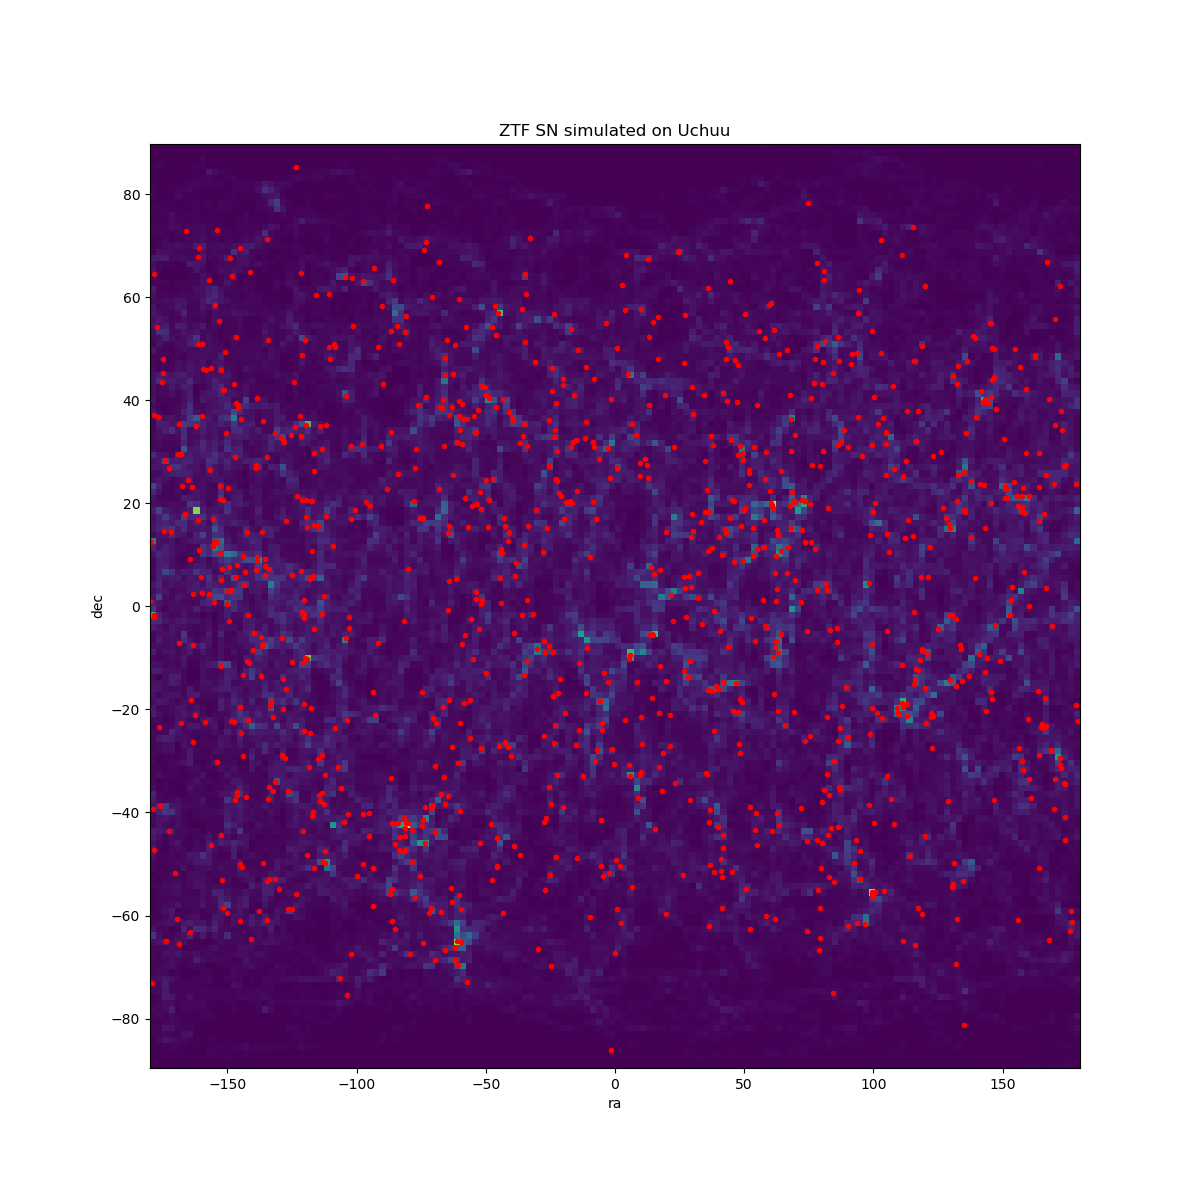
\includegraphics[width=0.9\textwidth]{MainLayout/BORG_chapter/figures/ztf_uchuu.png}
    \caption{2D full-sky projection of the Uchuu density field at redshift of $z\approx0.04$ with the ZTF supernovae simulated on top of it represented by red dots.}
    \label{fig:ztf_uchuu}
\end{figure}


\section{BORG-Peculiar Velocity}

The BORG-Peculiar Velocity (BORG-PV) algorithm is the same as the traditional BORG algorithm with the main difference being in the tracer modeling and likelihood. For BORG-PV, we 
will be using the supernovae distance moduli along with their redshifts as input. The goal will be to then infer the underlying density and velocity field as 
. One major difference with the study of galaxies is in the implementation of a bias model. 
The study of galaxy bias models has a long history with many different models having been suggested such as a linear bias (\cite{Kaiser_1984}), a nonlinear local bias (\cite{Fry_1993}) or an EFTofLSS bias (\cite{Mirbabayi_2015}) 
and there are still ongoing efforts to improve it. For the case of supernovae we will be relying on a simple phenomonological approach which will be describeed in the 
following section alongside the supernova modeling and likelihood. \\ 

\subsection{Initial likelihood}

In this section we will be describing the initial version of the BORG-PV likelihood. This likelihood was developped by Deaglan J. Bartelett during the beginning of my PhD
and it describes how well we can infer the supernova velocities. 
We denote $\mu_{\text{obs}}$ the observed distance modulus\footnote{As we explained in Chapter 2, we do not directly observe the distance modulus but instead it calculated through
the observations of supernova lightcurves. In here we assume that that $\mu_{\text{obs}}$ is the distance modulus obtained after having observed the supernova lightcurves.}, 
$z_{\text{obs}}$ the observed redshift and $\sigma_{\mu}$ is the intrinsic dispersion of supernovae. The first ingredient we need to determining the likelihood is having a prediction 
for the observed redshift. This should include the contribution of the supernova peculiar velocities with the help of the inferred velocity field. For objects at low redshift, 
Equation \ref{eqn:physical_distance} for comoving distances $r$ can be approximated as:
\begin{equation}
    r \approx \frac{c}{H_0} \left[ z - \frac{1+q_0}{2} z^2 \right]
\end{equation}
with $q_0 = \frac{\Omega_m}{2} - \Omega_{\Lambda} $. By inverting this relation for $z$, we get:
\begin{equation}
    z = \frac{1 - \sqrt{1 - 2rH_0(1+q_0)/c}}{1+q_0}
    \label{eqn:zcosmo}
\end{equation} 
For our analysis, we fix $H_0$ and $\Omega_{\Lambda}$ to a fiducial cosmology. We can then infer the cosmological redshift by knowing the distance $r$, 
given by inverting the luminosity distance relation in Equation \ref{eqn:dL_mu}, and $\Omega_m$. We 
will be denoting this redshift as $z_{\text{cosmo}}$. We can have a predicted redshift by adding the contribution of the velocity field using the following relation:
\begin{equation}
    cz_{\text{pred}}(r) = cz_{\text{cosmo}}(r) + (1+z_{\text{cosmo}}(r))v_r
\end{equation}
where $z_{\text{pred}}$ is the predicted redshift and $v_r$ is the radial projection of the velocity field at a distance $r$. We also assume that the peculiar velocities can be 
affected by sources other than the velocity field which will be modeled as a Gaussian noise $\mathcal{N}(0, \sigma_v)$.\\ 

The second ingredient would be to define a prior on the supernova distribution. If we assume a constant density of 
supernovae, than the expected number of supernova $N$ present at a distance $r$ is purely geometrical giving us:
\begin{equation}
    dN \propto 4\pi r^2 dr
\end{equation}
This means that the number of supernovae present between $r$ and $r+dr$ scales as $r^2$. Moreover, we define a supernova bias model relating the positions of supernovae with 
the evolved density field as:
\begin{equation}
    b_{SN}(r) = (1 + \delta^F(r))^{\alpha}
\end{equation}
where $\alpha$ is a free parameter. We'll call it the bias parameter. The bias parameter can exhibit four regimes:
\begin{itemize}
    \item $\alpha=0$: No bias exists and supernova do not preferential position regarding the dark matter field.
    \item $\alpha=1$: Supernova exhibits a linear bias where the number of supernova is proportional to the overdensities.
    \item $\alpha>1$: Supernova have a higher preference of being in overdense regions.
    \item $\alpha<1$: Supernova have a higher preference of being in underdense regions.
\end{itemize}
The prior on the supernova positions can then be written as:
\begin{equation}
    p_{SN}(r) = r^2 b_{SN}(r) = r^2 (1 + \delta^F(r))^{\alpha}
\end{equation}

Thirdly, we define a selection function that accounts for the fact that supernovae are not observed infinitely far away. For this, we use the following selection function:
\begin{equation}
    p_{\text{selection}}(r) = e^{-\lambda \frac{r}{R_{\text{max}}}}
\end{equation}
where $\lambda$ is a free parameter controlling the rate of decay and $R_{\text{max}}$ is the maximum comoving distance of the survey. 
This parametrisation allows for a smooth exponential decay of the expected number of supernovae with distance, avoiding the sharp 
discontinuity that would arise from a hard cutoff at $r = R_{\text{max}}$. \\

Finally, we marginalize over the distance $r$ for each supernova and normalize the likelihood, giving us:

\begin{equation}
    p(cz_{\text{obs}}|\mu_{\text{obs}})= \frac{\left( \int_{0}^{R_{\text{lim}}} dr \quad e^{- \frac{(\mu_{\text{pred}}(r) -\frac{\mu_{\text{obs}}}{\mu_A} )^2}{2\sigma_{\mu}^2} } 
    \quad e^{-\frac{(cz_{\text{pred}}(r) - cz_{\text{obs}})^2}{2 \sigma_v^2}} \quad p_{SN}(r) \quad e^{-\frac{\lambda}{R_{\text{max}}}r} \right)}{\left(\int_{0}^{R_{\text{lim}}} dr 
    \quad e^{- \frac{(\mu_{\text{pred}}(r) -\frac{\mu_{\text{obs}}}{\mu_A} )^2}{2\sigma_{\mu}^2} } 
    \quad p_{SN}(r) \quad e^{-\frac{\lambda}{R_{\text{max}}}r}\right)}
\end{equation}

Where $R_{\text{lim}}$ is the integration limit which is greater than the furthest supernova, $\mu_A$ the distance uncertainty and $\mu_{\text{pred}}(r)$ is calculated with:
\begin{equation}
    \mu_{\text{pred}}(r) = 5 \log_{10} \left( (1+z_{\text{cosmo}}(r))r \right) + 25
    \label{eqn:mu_r}
\end{equation}

\subsection{Generating self-consistent mocks}

The self-consistent supernova mocks are simulated to mach the model description above. We start by generating a random Gaussian initial density field $\delta^{IC}$ and let it evolve 
using a gravity solver until we obtain a final density field $\delta^{F}$ and a velocity field $\mathbf{v}$. We then define an amplitude function $\Phi$ containing the bias model and 
selection effects:
\begin{equation}
    \Phi(r, \phi, \theta) = (1+ \delta(r, \phi, \theta))^{\alpha}.e^{-\frac{\lambda}{R_{\text{max}}}r}
\end{equation}
The supernova are then generated by a Poisson process where a discrete generation of the cartesian coordinates from the amplitude function $\Phi$ is done. 
The number of supernovae generated is chosen beforehand. A mask is applied to ensure that the supernova generated are within the limit $R_{\text{lim}}$. We then 
calculated the observed redshift using:
\begin{equation}
    cz_{\text{obs}} = cz_{\text{cosmo}} + (1+z_{\text{cosmo}})v_r + \mathcal{N}(0, \sigma_v)
\end{equation}
where $z_{\text{cosmo}}$ is calculated using Equation \ref{eqn:zcosmo} and $v_r$ is the radial projection of the velocity field at $r$ for each supernova. The distance modulus 
is obtained the same way as Equation \ref{eqn:mu_r} and is then scattered so we get an observed distance modulus with:
\begin{equation}
    \mu_{\text{obs}} = \mu_{\text{true}} + \mathcal{N}(0, \sigma_{\mu})
\end{equation}
Finally, the right ascension and declanation angles are reported by converting the cartesian coordinates into spherical coordinates. \\

\subsection{Issues with intial likelihood}
\subsubsection{Selection function}

While testing different parameter configurations for the previously mentioned selection function, we have noticed a strong dependency in the $\lambda$ parameter that can bias the 
sampling of the other model parameters as well as the cosmology. We plot in Figure () the likelihood profile of a self-consistent simulation (see Section ref for more details on the 
simulation) for $\alpha$, the $z$-axis component of the bulkf flow $V_z$, $\Omega_m$ and $\sigma_8$ for 4 values of $\alpha$ : 1, 3, 5 and 7 while $R_{\text{max}}$ is 
fixed at $370 \text{Mpc}.h^{-1}$. 
What we notice is that all parameters are very sensitive to value of $\lambda$, more specifically that the smaller the value of $\lambda$, the more biased the parameters are. Therefore 
an incorrect initial estimation of $\lambda$ can be greatly problematic. Moreover, this choice of modeling will fail if we decide to apply our BORG-PV model on the ZTF DR2 volume 
limited sample as the selection function does not match the hard cutoff at a redshift of $z=0.06$. We can even attempt to set $\lambda$ to 0 since the volume limited sample 
should be a complete sample but this results in the same issue as seen in Figure (ref). \\

\subsubsection{Supernova prior}

Recent results from \cite{Lordet_2026} have shown that supernovae tend to be found in overly dense regions in the Universe with a large number of supernovae being present at a 
redshift of $z \approx 0.02-0.03$ creating what we see as a "bump" in the supernovae distribution accross redshift. This means that the assumption that the supernovae density is 
constant at low redshift (example of what was done in \cite{Perley_2020}) is not the most accurate description of the supernova distribution. The number of supernova 
$N_{\text{SN}}$ observed by a survey between a distance $r$ and $r+dr$ can be expressed as:
\begin{equation}
    dN = n(r) \times 4 \pi r^2 dr
\end{equation}
where $n(r)$ is the number density of supernovae. This can be related to the observed rate as:
\begin{equation}
    R(r) = \mathrm{S}(\phi, \theta, r) \frac{n(r)}{T_{\text{obs}}}
\end{equation}
where $T_{\text{obs}}$ is the time of observation and $\mathrm{S}$ is a selection function that would account for the survey's footprint, galactic extinction and any 
instrumental effects that would decrease the number of observed supernova. For our applications on self-consistent simulations and the 
ZTF-Uchuu mocks (Sections ref and ref), we will be generating supernovae on the full-sky and will not include any Malmquist bias effects. Therefore $\mathrm{S}$ becomes unity. 
If we assume a constant rate, then $dN \propto r^2 dr$ giving the $r^2$ geometric dependence in the prior described earlier. 
If we assume that this is not the case, then we get:
\begin{equation}
    dN(r) \propto n(r)r^2 dr
\end{equation}
In practice, we do not have direct access to $n(r)$ but we can infer $n(z)$. In Figure (ref) we show the $n(z)$ distribution obtained on the ZTF-Uchuu simulations obtained in 
100? bins up to a redshift of $z=0.06$. We proceed to then fit the number density with a cubic spline. The purpose of fitting with a cubic spline is to keep the $n(z)$ 
differentiable as it will be needed to then infer $n(r)$. In fact, we can relate the two number densities with:
\begin{equation}
    n(r) \propto \frac{n(z)}{4\pi r^2 \times \frac{dr}{dz}}
\end{equation}
The $\frac{dr}{dz}$ term can be deduced from Equation \ref{eqn:physical_distance} and is entirely determined by the cosmology. We get $\frac{dr}{dz} = \frac{c}{H(z)}$.
Finally, we can present a more realistic prior on supernovae expressed as:
\begin{equation}
    p_{SN}(r) \propto r^2\, n(r)\,(1+\delta^F)^{\alpha},
    \quad \text{with } n(r) \propto \frac{n(z)}{4\pi r^2 \times \frac{dr}{dz}}.
    \label{eqn:new_prior}
\end{equation}

Other motivations for this new prior lies in the ZTF-Uchuu simulations themselves. We could assume that such effects can be captured by the bias model. We 
compare self-consistent simulations with the ZTF-Uchuu simulations containing the exact same number of supernovae. We generated a set of self-consistent mocks each with 
a different value for $\alpha$. We bin the number of supernovae based on the overdensity. If the simulations are generated in the same way, we would expect to see 
a match between the bins for a given $\alpha$ value. We obtain the following Figures (ref). We notice that there isn't a singular value of $\alpha$ for which the 
self consistent simulations match the ZTF-Uchuu simulations. Moreover, we seem to notice a regime change based on the over density for the ZTF-Uchuu simulations, which 
could possibly hint that the difference can be capured using two bias model parameters. During this PhD I have not explored this avenue but instead relied on the new supernova 
prior to capture the differences between the simulations. \\



\subsection{Improved likelihood}

Our first improvement to the likelihood is in the implementation of the prior presented in Equation \ref{eqn:new_prior}. The second improvement was done by replacing the 
selection function $p_{\text{selection}}(r)$. We were inspired by the work done in \cite{Stiskalek_2025}. The method derived in the paper largely follows what was done in \cite{Kelly_2008}. Given a 
an observed dataset $\mathbf{d}_i$ for a source $i$ with source parameters $\boldsymbol{\theta}_i$ drawn from a population characterized by $\boldsymbol{\Lambda}$ 
and a selection function $S$ such that $S=1$ is the data is observed and $S=0$ if not, then the fraction of detected samples from a total population is given by:
\begin{equation}
    p(S=1|\boldsymbol{\Lambda}) = \int \int d \mathbf{d}_{\text{pred}} d \boldsymbol{\theta} p(S=1|\mathbf{d}_{\text{pred}}) \mathcal{L} 
    (\mathbf{d}_{\text{pred}}|\boldsymbol{\theta}, \boldsymbol{\Lambda})\pi (\boldsymbol{\theta}|\boldsymbol{\Lambda})
\end{equation}
where $\mathbf{d}_{\text{pred}}$ denotes the predicted data vector and $\pi$ the prior as detailed in Equation (21) of the paper. The paper to give the exact formulation when 
the selection is done on redshift, which is exactly the case for the ZTF DR2 volume limited sample. In that case, the fraction of detected samples 
is given by Equation (33) in the paper:
\begin{equation}
    p(S=1) = \int d^3 \mathbf{r} p_{SN}(\mathbf{r}) \Phi_{\text{CDF}} \left(\frac{cz_{\text{thresh}} - cz_{\text{pred}(r)}}{\sigma_v}\right)
\end{equation}
where $z_{\text{thresh}}$ is the limiting redshift ($z_{\text{thresh}}=0.06$ in our case) and $\Phi_{\text{CDF}}$ the normal cumulative distribution function. The full likelihood 
is therefore given by:
\begin{equation}
    \mathcal{L} = \prod_{i=1}^{N_\text{SN}} p(cz_{\text{obs},i}|\mu_{\text{obs},i})p(S=1)
\end{equation}
Where $i$ denotes each individual supernova. Or more simply, we can take the natural logarithm of the likelihood which gives us:
\begin{equation}
    \boxed{\log \mathcal{L} = \sum_{i=1}^{N_\text{SN}} p(cz_{\text{obs},i}|\mu_{\text{obs},i}) + N_\text{SN}p(S=1)}
\end{equation}
Where $p(cz_{\text{obs}_i}|\mu_{\text{obs}_i})$ is the likelihood of each supernova with no selection effects which is given by
\begin{equation}
    \boxed{p(cz_{\text{obs}_i}|\mu_{\text{obs}_i}) = \int_{0}^{R_{\text{lim}}} dr \quad e^{- \frac{(\mu_{\text{pred},i}(r) -\frac{\mu_{\text{obs},i}}{\mu_A} )^2}{2\sigma_{\mu}^2} } 
    \quad e^{-\frac{(cz_{\text{pred},i}(r) - cz_{\text{obs},i})^2}{2 \sigma_v^2}} \quad r^2\, n(r)\,(1+\delta^F(r))^{\alpha}}
\end{equation}
\section{Applications on self-consistent mocks}
\section{Applications on Uchuu-ZTF Mocks}

\subsection{Uchuu-ZTF Mocks} \label{sec:uchuu_ztf}

The ZTF simulations are designed to test the impact of ZTF-supernovae peculiar velocities in a cosmological analysis are called DC PV (Data Challenge 
Peculiar Velocity). These are generated within the ZTF collaboration mainly to test the methods to infer $f\sigma_8$. 
The DC PV simulations are done similarly to the DC simulations  
described in Chapter 4 with the main differences being that supernovae are simulated on top of large scale structures instead of a uniform distribution. 
For that, we use the Uchuu N-body simulation 
(\cite{Ishiyama_2021}), a high fidelity N-body dark matter simulation\footnote{N-body and hydrodynamical simulations 
are considered the highest fidelity simulations we can get to describe structure formation as they solving the equations of motion for each particle/fluid without any 
approximations or grid mesh} 
in a $(2 \text{Gpc}.h^{-1})^3$ box with 2.1 trillion particles that can be seen in Figure \ref{fig:uchuu_nbody} . 
The full box is then subdivided into 27 subboxes where the supernovae are simulated up to a redshift of $z=0.11$, giving 27 quasi-independent 
realizations of the DC PV. 
Each supernova is simulated at the location of a dark matter halo is and is assigned the halo's velocity. This allows us to add proper motion to supernovae 
that is driven by structure formation.\\

\begin{figure}[ht]
    \centering
    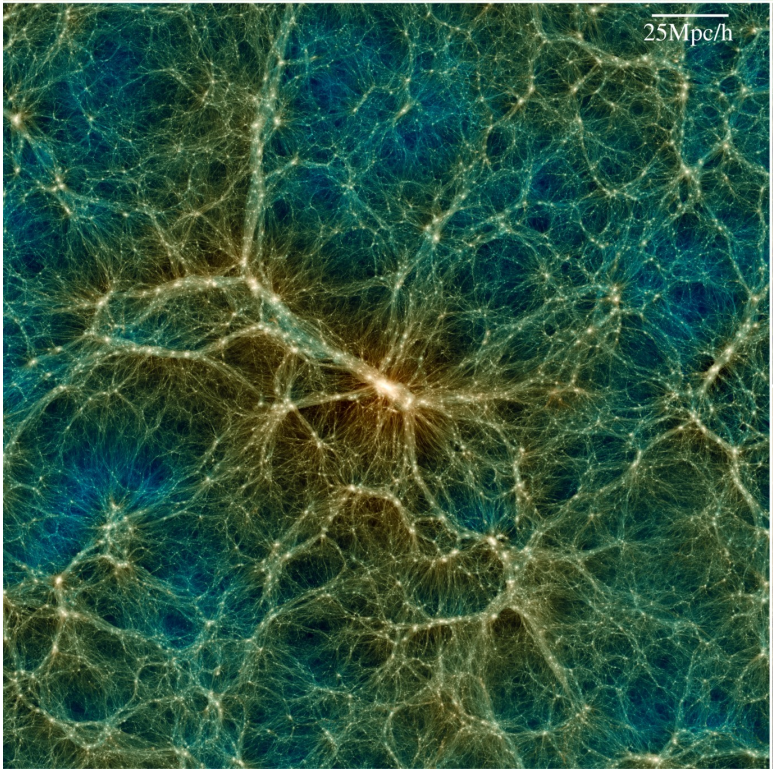
\includegraphics[width=0.7\textwidth]{MainLayout/BORG_chapter/figures/uchuu_nbody.png}
    \caption{Slice taken from the Uchuu simulation covering a box of 250 $\text{Mpc}.h^{-1}$ where each point represents a particle. Taken from \cite{Ishiyama_2021}}
    \label{fig:uchuu_nbody}
\end{figure}


We opt to simplify a few aspects of the simulations in order to have an initial assessment of how well can a BORG analysis run on ZTF-like supernova. 
Firstly, we have chosen to use only the distance moduli and redshifts of supernovae as inputs in BORG, as if we were doing the analysis after having run the full 
LEMAITRE pipeline. 
One could also infer the Tripp relation parameters ($\alpha_{\text{Tripp}}$, $\beta_{\text{Tripp}}$) in BORG. 
Performing this inference at the BORG level would offer an 
additional advantage: the 3-dimensional reconstruction of the matter 
distribution in the nearby Universe provides a 
correction for inhomogeneous Malmquist bias. In standard analyses, 
Malmquist bias corrections rely on an assumed homogeneous distribution 
of matter, which can introduce systematic errors in underdense and 
overdense regions. Within BORG, the reconstructed density field 
directly encodes the inhomogeneous matter distribution along each line 
of sight, allowing a more accurate correction for the preferential 
detection of supernovae in overdense environments near the survey 
boundary.
Secondly, we do not impose the ZTF DR2 cosmology quality cuts on photometry nor the ZTF footprint, so all of the supernovae that are 
generated can be used. 
For a more realistic set of simulations, we would have to account for the geometry of the survey as well as the Milky-Way dust. This is trivial to account for, but 
for simplicity we opted not to include it. 
It consists in introducing an 
angular mask $M(\text{RA}, \text{Dec})$ in the likelihood's selection function. 
This method was applied in BORG analyses such as 
\cite{Mcalpine_2025} (Manticore-Local) and \cite{Mcalpine_2026} (Manticore-Deep). 
Finally, we simulate ZTF-like supernova up to a redshift of $z=0.11$ and draw a set of 1000 randomly selected supernovae whose observed redshift goes up to $z=0.06$ in order to 
match the expected number of supernovae in the volume-limited sample from ZTF. \\

\subsection{Forward Model Analysis: Likelihood Profile Test}

The methodology used to generate supernova in the self consistent simulations and DC PV are different as we have mentioned earlier. We want to ensure that we can 
quantify any systematic biases introduced by those differences. To do this, we start by generating an initial density field using BORG $\delta^{\text{BORG}}_{IC}$ using a 
Planck18 cosmology (\cite{Planck_2018_params}) and known bulk flow $\mathbf{V}$. The configuration of the generated field is given in Table \ref{tab:borg_nbody}. 
We then let that field evolve using LPT gravity model to obtain the evolved density field 
$\delta^{\text{BORG}}_{F}$ and velocity field $\mathbf{v}^{\text{BORG}}_{IC}$. The ZTF simulations are designed to generate the supernovae on top of an N-body simulation, so 
from the evolved density field we create a "synthetic" N-body simulation. The simplest way to do so is to take each voxel-$i$ and generate within it $N_i$ particles proportional 
to $(1+\lceil \delta^{\text{BORG}}_{F}\rceil )_i$ where $i$ denotes the voxel index. We take the ceiling of the evolved density field to ensure we get an integer number of 
particles and to have at least 1 particle in empty voxels. We also generate fewer particles than in the Uchuu simulation, around 2 million, due to memory and storage limiations. \\

\begin{table}[ht]
    \centering
    \caption{Set of parameters used to generate the "synthetic" N-body BORG simulation.}
    \label{tab:borg_nbody}
    \begin{tabular}{|l|c|}
        \hline
        Parameters & Values \\
        \hline
        Box size & $700^3 \, (\text{Mpc}.h^{-1})^3$ \\
        Generated supernovae & $\sim 1000$ \\
        Maximum supernova redshift & $z=0.06$ \\
        Gravity model & COLA \\
        Resolution & 10.9 $\text{Mpc}.h^{-1}$ \\
        $V_x$ & 0 km/s \\
        $V_y$ & 0 km/s \\
        $V_z$ & 0 km/s \\
        $\Omega_m$ & 0.31 \\
        $\sigma_8$ & 0.81 \\
        \hline
    \end{tabular}
\end{table}
We then use this "synthetic" N-body simulation to generate ZTF-like supernovae using skysurvey (\cite{Rigault_2026}) and then evaluate the BORG-supernova likelihood (Equation \ref{eqn:borg_pv_L}) 
while varying the cosmological and model parameters in BORG. We create a likelihood profile for each parameter, not only to 
determine whether the ZTF-like supernova simulations introduce systematic biases in BORG but also to help us understand how we can relate some of the BORG-supernova model 
parameters, 
such as $\alpha$ and $\sigma_v$ to the ZTF simulations as they are not explicitly specified. \\

We obtain the following likelihood profiles for one synthetic N-body simulation in Figures \ref{fig:cosmo_lpt_L}, \ref{fig:params1_lpt_L}, \ref{fig:params2_lpt_L} and \ref{fig:params3_lpt_L}. We notice that the cosmological parameters $\Omega_m$ and $\sigma_8$ are unbiased and we recover the 
input cosmology. The bulk flow $V$ parameters are compatible with 0 km/s, indicating that no additional bulk flow is added within the ZTF simulation. 
The bias model parameter $\alpha$ 
seems to prefer values around $0.9 -1.0$. 
This is not unexpected, if we assume that the ZTF supernova are generated where there are dark matter particles without a preference on whether 
then the number of supernovae would simply scale as $\delta_F$. 
The velocity dispersion is preferred around $200$ km/s. 
The $\mu_A$ parameter seem to prefer a value of $1.0$, meaning no additional sources of uncertainty are added to the distance modulus.

\begin{figure}
    \centering
    \begin{subfigure}{0.45\textwidth}
        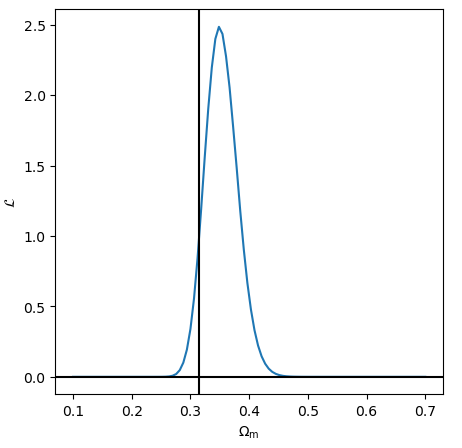
\includegraphics[width=\textwidth]{MainLayout/BORG_chapter/figures/omega_m_L.png}
        \caption{Likelihood profile for $\Omega_m$}
        \label{fig:omega_m_lpt_L}
    \end{subfigure}
    \hfill
    \begin{subfigure}{0.45\textwidth}
        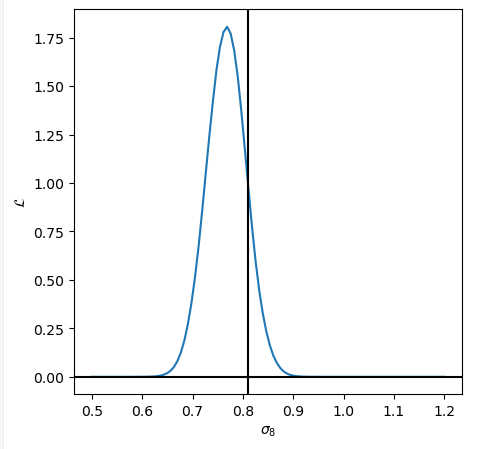
\includegraphics[width=\textwidth]{MainLayout/BORG_chapter/figures/sigma_8_L.png}
        \caption{Likelihood profile for $\sigma_8$}
        \label{fig:sigma8_lpt_L}
    \end{subfigure}
    \caption{Likelihood profiles of the cosmological parameters for a synthetic N-body simulation generated with LPT}
    \label{fig:cosmo_lpt_L}
\end{figure}

\begin{figure}
    \centering
    \begin{subfigure}{0.45\textwidth}
        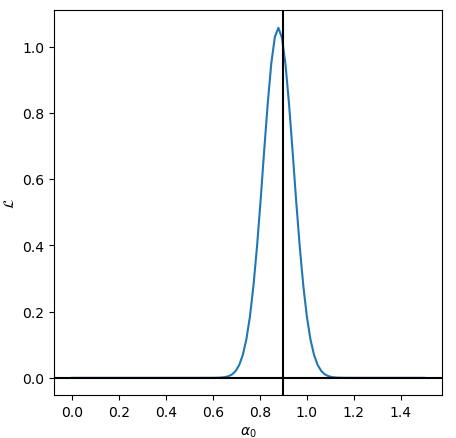
\includegraphics[width=\textwidth]{MainLayout/BORG_chapter/figures/alpha_L.png}
        \caption{Likelihood profile for $\alpha$}
        \label{fig:alpha_lpt_L}
    \end{subfigure}
    \hfill
    \begin{subfigure}{0.45\textwidth}
        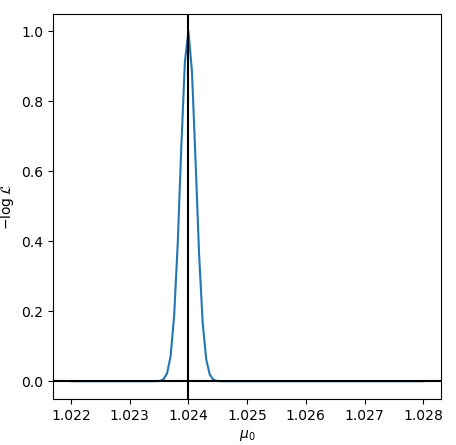
\includegraphics[width=\textwidth]{MainLayout/BORG_chapter/figures/muA_L.png}
        \caption{Likelihood profile for $\mu_A$}
        \label{fig:muA_lpt_L}
    \end{subfigure}
    \caption{Likelihood profiles of $\alpha$ and $\mu_A$ for a synthetic N-body simulation generated with LPT}
    \label{fig:params1_lpt_L}
\end{figure}

\begin{figure}
    \centering
    \begin{subfigure}{0.45\textwidth}
        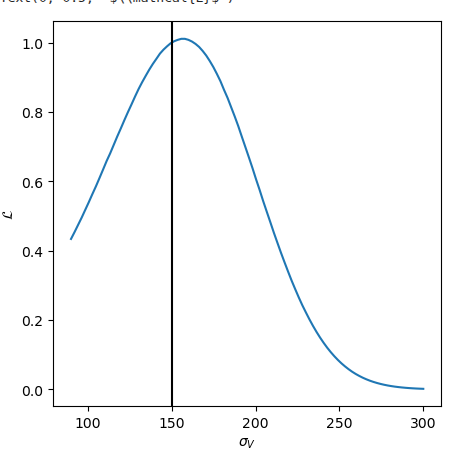
\includegraphics[width=\textwidth]{MainLayout/BORG_chapter/figures/sigma_v_L.png}
        \caption{Likelihood profile for $\sigma_v$}
        \label{fig:sigma_v_lpt_L}
    \end{subfigure}
    \hfill
    \begin{subfigure}{0.45\textwidth}
        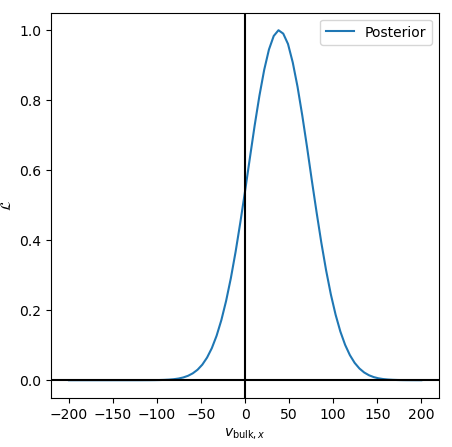
\includegraphics[width=\textwidth]{MainLayout/BORG_chapter/figures/bulk_x_L.png}
        \caption{Likelihood profile for $V_x$}
        \label{fig:Vx_lpt_L}
    \end{subfigure}
    \caption{Likelihood profiles $\sigma_v$ and $V_x$ for a synthetic N-body simulation generated with LPT}
    \label{fig:params2_lpt_L}
\end{figure}

\begin{figure}
    \centering
    \begin{subfigure}{0.45\textwidth}
        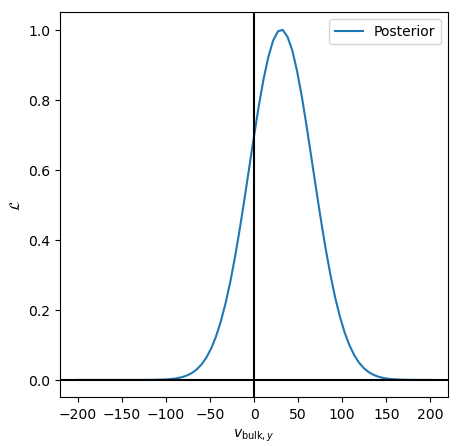
\includegraphics[width=\textwidth]{MainLayout/BORG_chapter/figures/bulk_y_L.png}
        \caption{Likelihood profile for $V_y$}
        \label{fig:Vy_lpt_L}
    \end{subfigure}
    \hfill
    \begin{subfigure}{0.45\textwidth}
        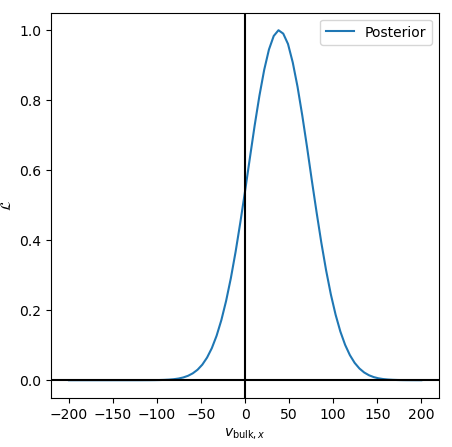
\includegraphics[width=\textwidth]{MainLayout/BORG_chapter/figures/bulk_x_L.png}
        \caption{Likelihood profile for $V_z$}
        \label{fig:Vz_lpt_L}
    \end{subfigure}
    \caption{Likelihood profiles $V_z$ and $V_z$ for a synthetic N-body simulation generated with LPT}
    \label{fig:params3_lpt_L}
\end{figure}

\section{Results of the field level inference on Uchuu-ZTF simulations}

We present in this section the results obtained on the DC PV. The procedure follows closely what was done on the self consistent simulations. 
The priors set on the parameters are:
\begin{itemize}
    \item $\alpha \sim \mathcal{U}[0.5, \, 2.5]$
    \item $\mu_A \sim \mathcal{U}[0.5, \, 1.5]$
    \item $\sigma_v \sim \mathcal{U}[50, \, 400] \, \text{km.s}^{-1}$
    \item Each bulk flow component $\sim \mathcal{U}[-200, \, +200] \, \text{km.s}^{-1}$ 
    \item $\Omega_m \sim \mathcal{U}[0.1, \, 0.8]$
    \item $\sigma_8 \sim \mathcal{U}[0.1, \, 1.5]$
\end{itemize}

The inference runs in four steps: 
\begin{enumerate}
 \item An initial warm-up phase is dedicated to sample the initial density perturbations $\delta^{IC}$ while all of other parameters are fixed using an LPT gravity solver. 
 This is done in 1000 MCMC steps.
 \item The following step we simultaneously $\delta^{IC}$ alongside nuisance and model parameters, specifically 
 $\sigma_v$, bulk flow, $\alpha$ and $\mu_A$ also using LPT. This is done for 3000 MCMC steps. 
 \item We keep on sampling the same parameters but switch to COLA for the gravity solver. The idea is that since LPT is much faster than COLA, to use it to initially guess some 
 of the model parameters so that sampling the parameters is then easier with COLA. For this run, it was done for 800 MCMC steps. 
 \item Lastly, we sample all of the parameters simultaneously including $\Omega_m$ and $\sigma_8$ using COLA. This step 
 takes a lot of computational on CPU. A converged state would be achieved during the timeline of this PhD. Efforts to parallelize the computations on GPUs is ongoing to accelerate this step.
\end{enumerate}
In Figure \ref{fig:dens_ztf_evolution} we display the evolution of the mean density field $\delta^{F}$ within a slice at the center of the box.


First, we present the results obtained when using the LPT gravity solver. 
We show in Figures \ref{fig:ztf_dens} slices of the final reconstructed density field with BORG in comparison with the Uchuu 
density. The red-dashed circle represents the limit of where the supernova are being generated (up to $z=0.06$). \\

\begin{figure}[htpb]
    \centering
    \begin{subfigure}{1\textwidth}
        \centering
        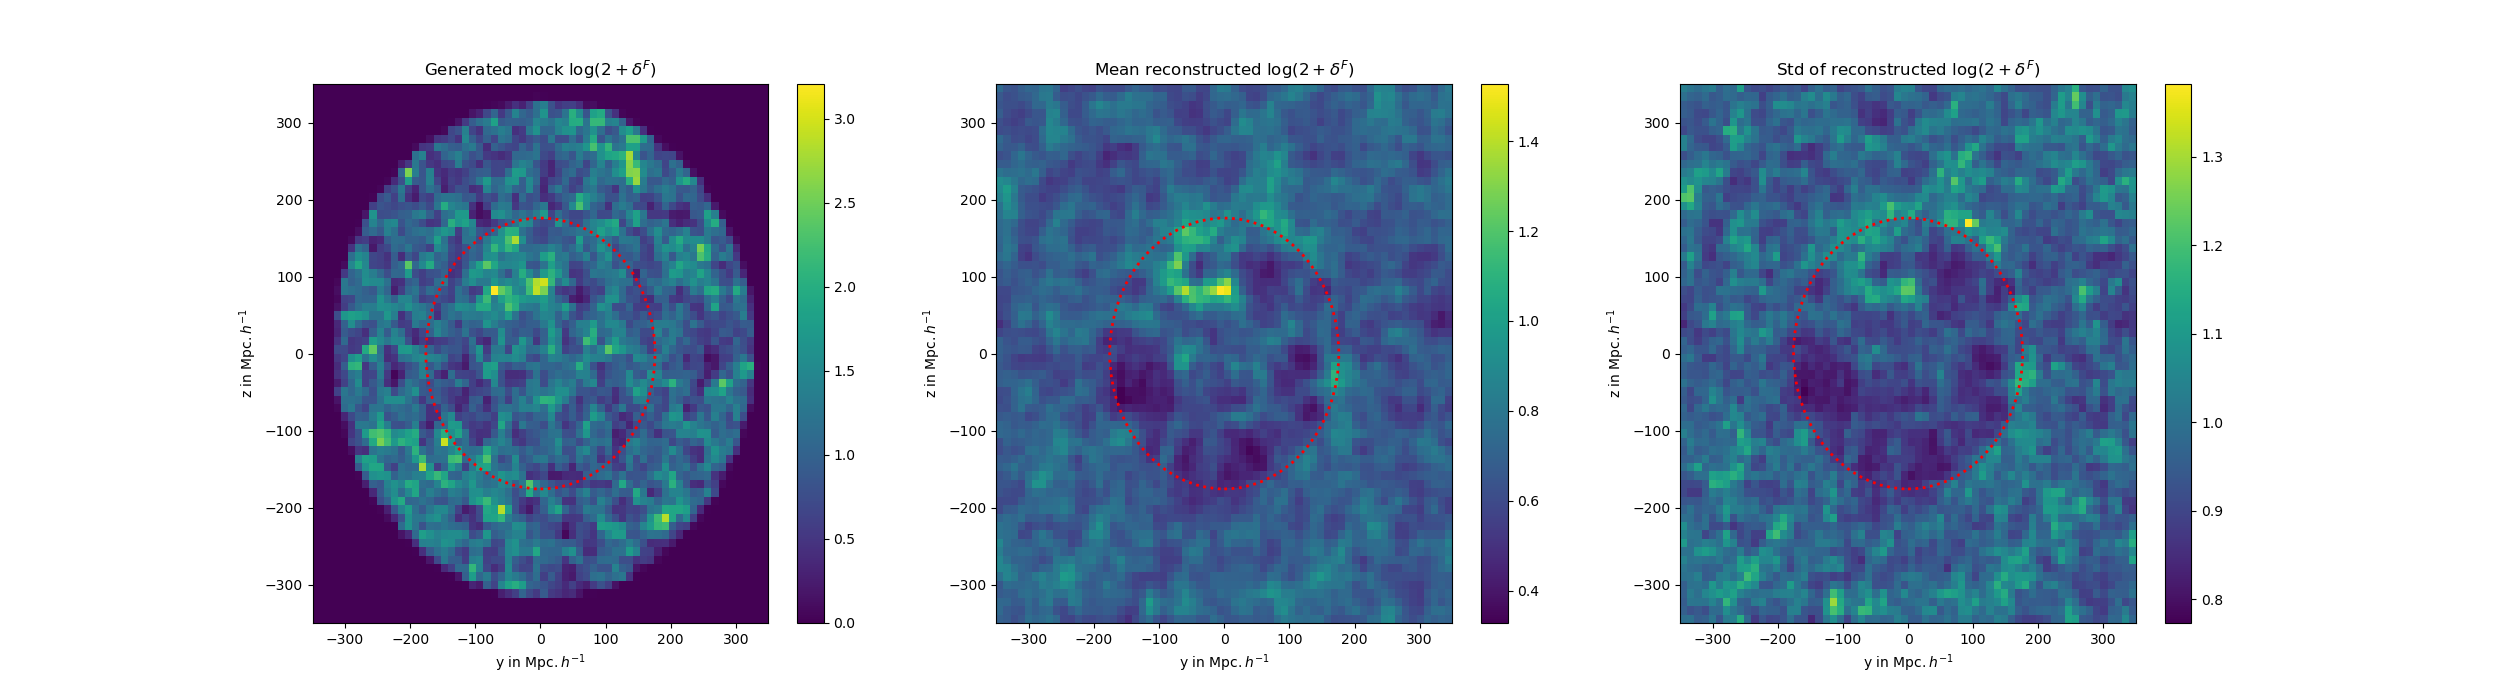
\includegraphics[width=1.2\textwidth]{MainLayout/BORG_chapter/figures/dens_slice_x_28.png}
        \caption{}
        \label{fig:ztf_dens_1}
    \end{subfigure}%
    
    \vspace{1em}
    
    \begin{subfigure}{1\textwidth}
        \centering
        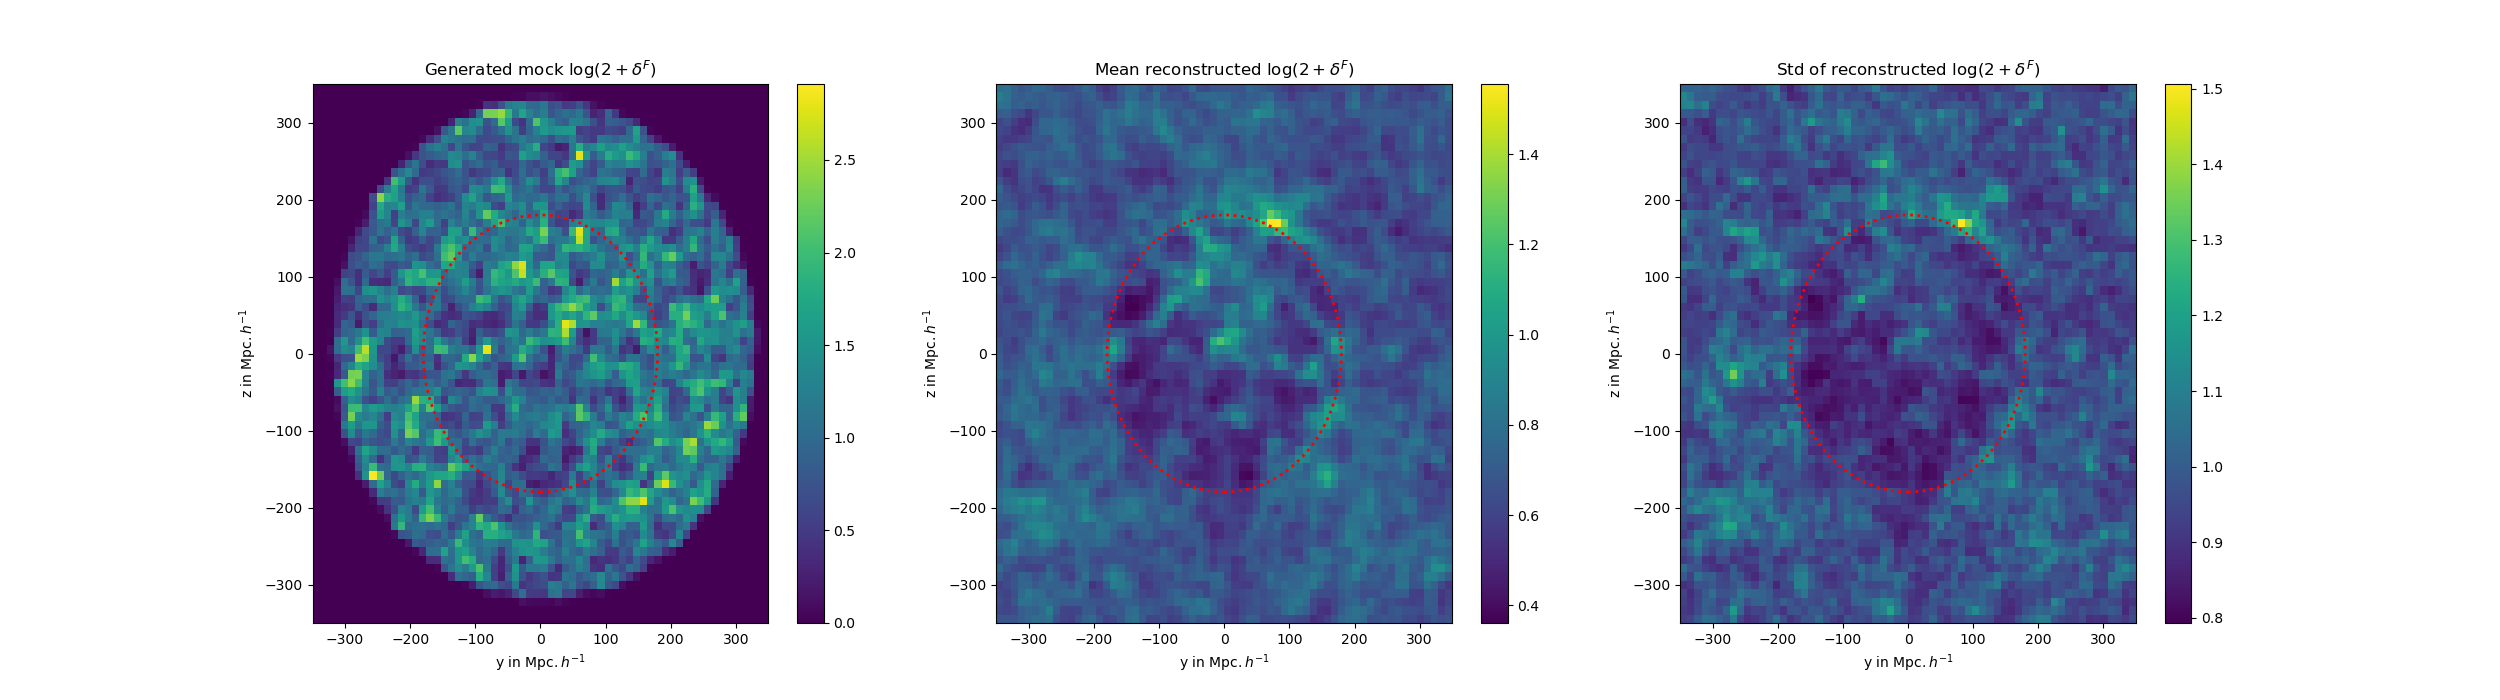
\includegraphics[width=1.2\textwidth]{MainLayout/BORG_chapter/figures/dens_slice_x_32.png}
        \caption{}
        \label{fig:ztf_dens_2}
    \end{subfigure}
    \caption{Slices of the density field from Uchuu and BORG reconstruction after having gone a CIC mass assignment. 
    The left column shows the Uchuu density field. The center column shows the mean posterior from BORG. 
    The right column shows the standard deviation. Each row is a different slice in the box.}
    \label{fig:ztf_dens}
    \end{figure}


We notice that the field reconstructed with BORG-PV manages to capture 
some of the underlying structure visible in Uchuu by comparing the overdense and underdense regions within the red-dashed circle. 
Notably, it is the largest structures that are 
recovered while smal scales structures seem to be missed. 
We show in Figures \ref{fig:ztf_vel} slices of the final reconstructed velocity field with BORG in comparison with the Uchuu 
velocity. \\ 

\begin{figure}[htpb]
    \centering
    \begin{subfigure}{1\textwidth}
        \centering
        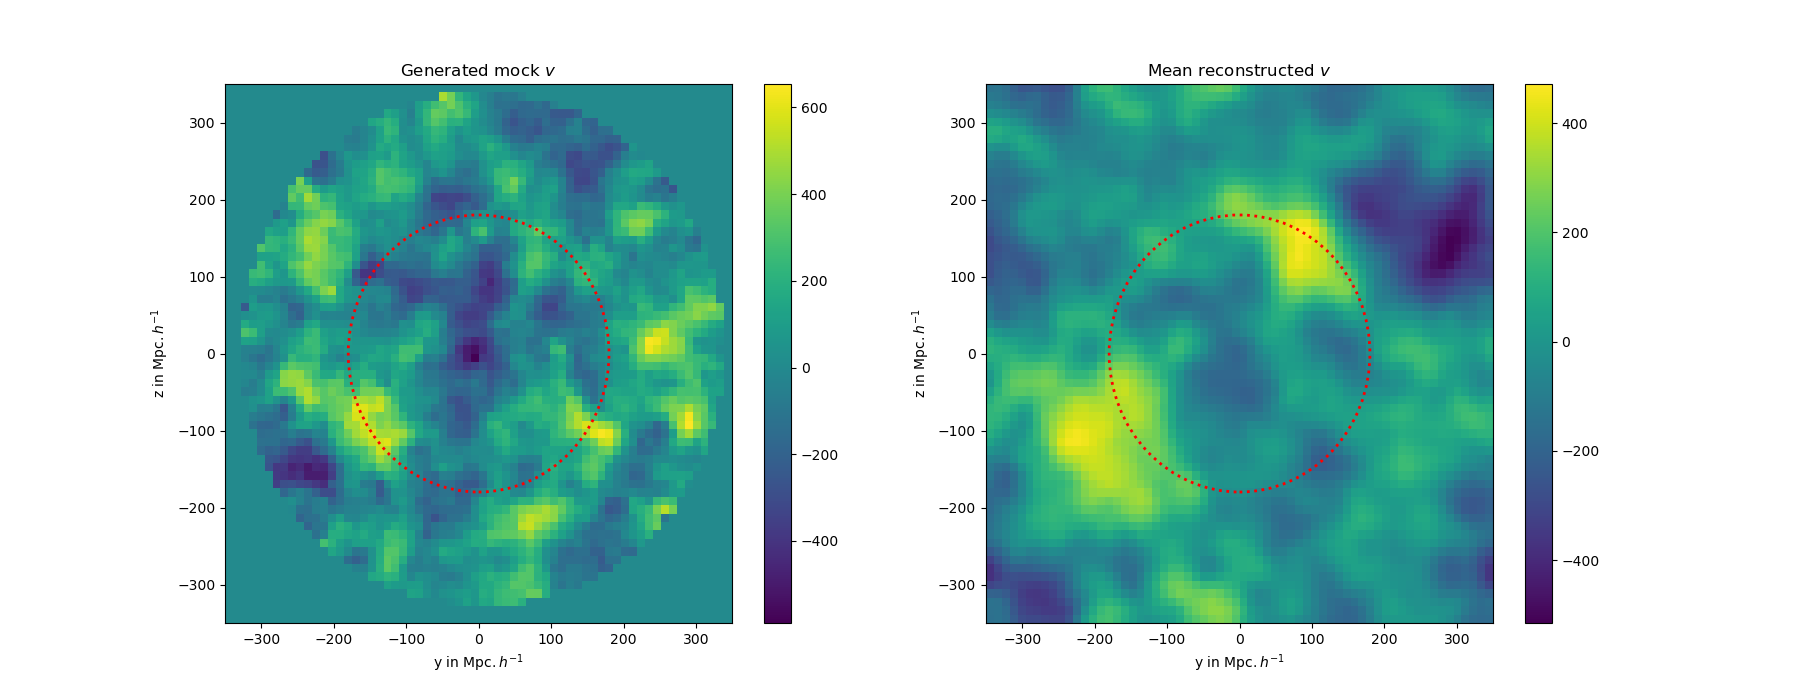
\includegraphics[width=1.0\textwidth]{MainLayout/BORG_chapter/figures/vel_slice_x_32.png}
        \caption{}
        \label{fig:ztf_vel_1}
    \end{subfigure}%
    
    \vspace{1em}
    
    \begin{subfigure}{1\textwidth}
        \centering
        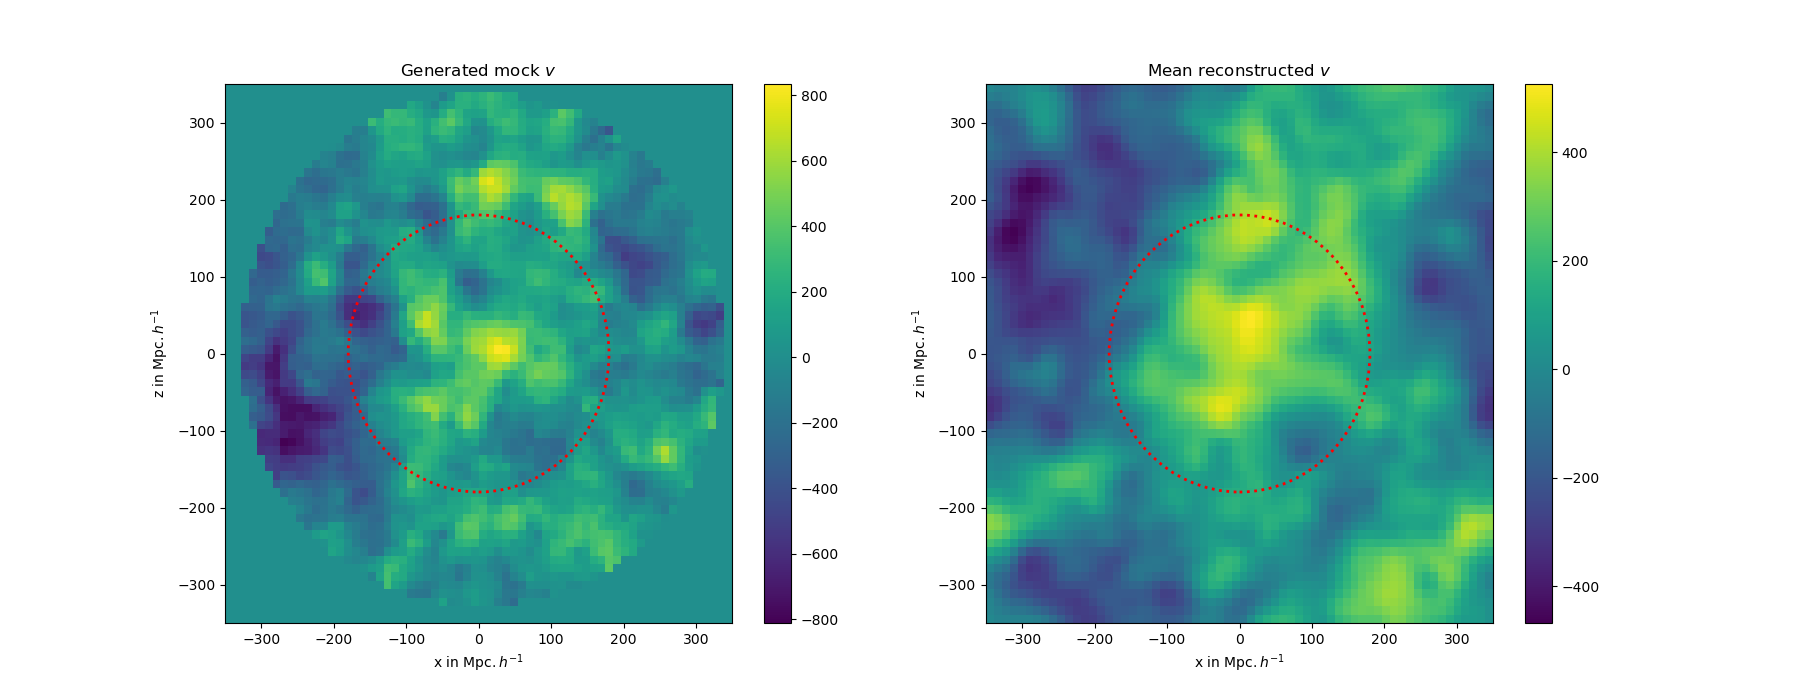
\includegraphics[width=1.0\textwidth]{MainLayout/BORG_chapter/figures/vel_slice_y_32.png}
        \caption{}
        \label{fig:ztf_vel_2}
    \end{subfigure}
    \caption{Slices of the velocity field from Uchuu and BORG reconstruction after having gone a CIC mass assignment. 
    The left column shows the Uchuu velocity field. The reight column shows the mean posterior from BORG. 
    Each row is a different slice in the box. The first row is a slice in the $x$ axis. The second row is a slice in the $y$ axis.}
    \label{fig:ztf_vel}
    \end{figure}



Similarly to the density field reconstruction, the BORG velocity field seems to match the Uchuu velocity at large scales. 
It is important to note that the velocity field 
is known to be more linear and Gaussian than the density field. 

---More results needed from here on out
To quantify this, we compare the power spectra of the density and velocity field components $v_x$, $v_y$ and $v_z$ from Uchuu to the one inferred by BORG in Figures (ref) as well 
as the cross correlation factor between them $r$ in Figures (ref). 
We notice that the power spectrum of the matter density matches the Uchuu power spectrum up to a wavenumber of $k \approx$. For the velocity fields we notice a matching result up 
to a wavenumber of $k \approx$. This confirms our qualitative results mentioned previously when looking directly at the reconstructed fields. \\

%Secondly we look at the sampled parameters. \\


%NEED SOME COLA RESULTS TO BETTER WRITE OFF THIS PART

%- results
% - covariance additions ?
% - full dataset with selection?

%\section{BONUS IF THERE IS TIME: Comparison with other methods for $f\sigma_8$}

%\textit{As with the self consistent simulation, we are restricted to a $\Lambda-CDM$ cosmology. Therefore if assume that $f\sigma_8$ is expressed as:}
%\begin{equation}
%    f \sigma_8 = \Omega_m^{0.55} \sigma_8
%\end{equation}
%\textit{by calculating this quantity, we can compare with other methods within the ZTF collaboration used to calculate $f\sigma_8$. Currently there is one ongoing work in doing so conducted by 
%Rafel Kebadian (Kebadian et al. in prep) where $f\sigma_8$ is determined using a maximum likelihood method on the DC PV supernovae. We present in Figure (ref) the results from the different methods. 
%We (hope) to see that using a field-level inference we obtain tighter constraints on $f\sigma_8$. However as mentioned before, we are limited to $\Lambda$CDM, so any deviations from 
%the expected value do not indicate what the strength of the underlying gravitational theory should be as much as it is a test on knowing whether the assumed gravitational theory (GR) 
%is correct or not. The maximum likelihood method however does not present that issue, but the $f\sigma_8$ constraints are looser.}
%\section{ZTF peculiar velocity data challenge (DC PV)}
 - Simulation description and volume limited sample


%\section{Supernova forward-model analysis}

The methodology used to generate supernova in the self consistent simulations and DC PV are different as we have mentioned earlier. We want to ensure that we can 
quantify any systematic biases introduced by those differences. To do this we start by generating an intial density field using BORG $\delta^{\text{BORG}}_{IC}$ using a 
Planck18 cosmology (\cite{Planck_2018_params}) and known bulk flow $\mathbf{V}$. The configuration of the generated field is given in Table \ref{tab:borg_nbody}. 
We then let that field evolve using the LPT gravity model giving us the evolved density field 
$\delta^{\text{BORG}}_{F}$ and velocity field $\mathbf{v}^{\text{BORG}}_{IC}$. The ZTF simulations are designed to generate the supernovae on top of an N-body simulation, so 
from the evolved density field we create a "synthetic" N-body simulation. The simplest way to do so would be taking each voxel-$i$ and generate within it $N_i$ particles proportional 
to $(1+\lceil \delta^{\text{BORG}}_{F}\rceil )_i$ where $i$ denotes the voxel's index. We take the cieling of the evolved density field to ensure we get an integer number of 
particles and to have at least 1 particle in empty voxels. We also generate less particles than the Uchuu simulation, around 200 million, due to memory and storage limiations. \\

\begin{table}[ht]
    \centering
    \caption{Set of parameters used to generate the "synthetic" N-body BORG simulation.}
    \label{tab:borg_nbody}
    \begin{tabular}{|l|c|}
        \hline
        Parameters & Values \\
        \hline
        Gravity model & LPT \\
        $V_x$ & 0 km/s \\
        $V_y$ & 0 km/s \\
        $V_z$ & 0 km/s \\
        $\Omega_m$ & 0.315 \\
        $\sigma_8$ & 0.81 \\
        \hline
    \end{tabular}
\end{table}
We then use this "synthetic" N-body simulation to generate ZTF-like supernova and then evaluate the BORG-supernova likelihood described in Equation (ref) 
while varying the cosmological and model parameters in BORG. Essentially creating a likelihood profile for each parameter. This is particularly important not just to 
determine whether the ZTF-like supernova simulations introduce systematic biases in BORG but also help us understand how we can relate some of the BORG-supernova model packagesarameters, 
such as $\alpha$ to the ZTF simulations as they are not explicitly specified. \\

We obtain the following likelihood profiles for 1 synthetic N-body simulation in Figures \ref{fig:cosmo_lpt_L}, \ref{fig:params1_lpt_L}, \ref{fig:params2_lpt_L} and \ref{fig:params3_lpt_L}. We notice that the cosmological parameters $\Omega_m$ and $\sigma_8$ are unbiased and we recover the 
input cosmology. The bulk flow $V$ parameters are compatible with 0 km/s, indicating that no additional bulk flow is added with the ZTF simulation. The bias model parameter $\alpha$ 
seems to prefer values around $0.9 -1.0$. This is not unexpected, if we assume that the ZTF supernova are generated where there are dark matter particles without a preference on whether 
then the number of supernovae would simply scale as $\delta_F$. The velocity dispersion is prefered around $150$ km/s with a large scatter. Measurements from (ref smth regarding sigv like velocity olympics) 
getting such values is possible and is indeed physical. The $\mu_A$ parameter seem to prefer a value of $1.024$ indicating that an offset of about $2.4\%$ regarding how distances are described in BORG. 
(check where does it come from but it is not an issue for our needs).

\begin{figure}
    \centering
    \begin{subfigure}{0.45\textwidth}
        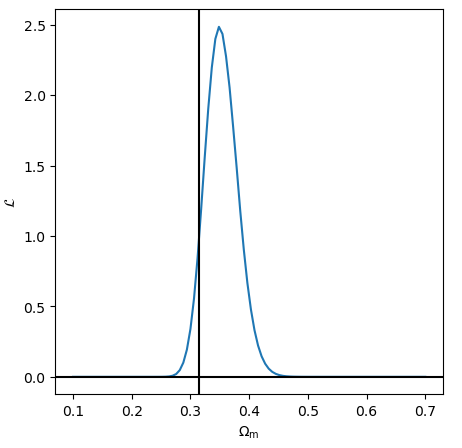
\includegraphics[width=\textwidth]{MainLayout/BORG_chapter/figures/omega_m_L.png}
        \caption{Likelihood profile for $\Omega_m$}
        \label{fig:omega_m_lpt_L}
    \end{subfigure}
    \hfill
    \begin{subfigure}{0.45\textwidth}
        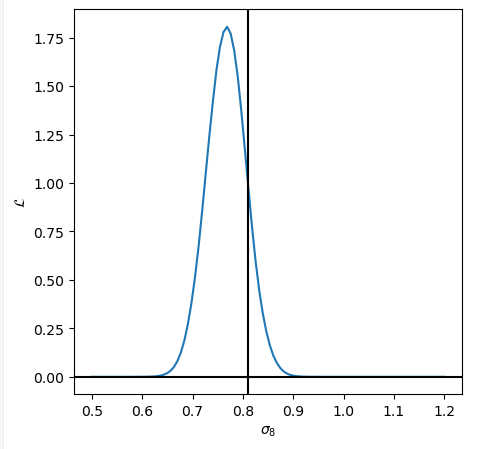
\includegraphics[width=\textwidth]{MainLayout/BORG_chapter/figures/sigma_8_L.png}
        \caption{Likelihood profile for $\sigma_8$}
        \label{fig:sigma8_lpt_L}
    \end{subfigure}
    \caption{Likelihood profiles of the cosmological parameters for a synthetic N-body simulation generated with LPT}
    \label{fig:cosmo_lpt_L}
\end{figure}

\begin{figure}
    \centering
    \begin{subfigure}{0.45\textwidth}
        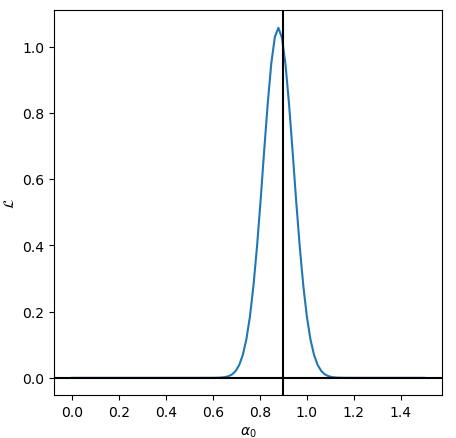
\includegraphics[width=\textwidth]{MainLayout/BORG_chapter/figures/alpha_L.png}
        \caption{Likelihood profile for $\alpha$}
        \label{fig:alpha_lpt_L}
    \end{subfigure}
    \hfill
    \begin{subfigure}{0.45\textwidth}
        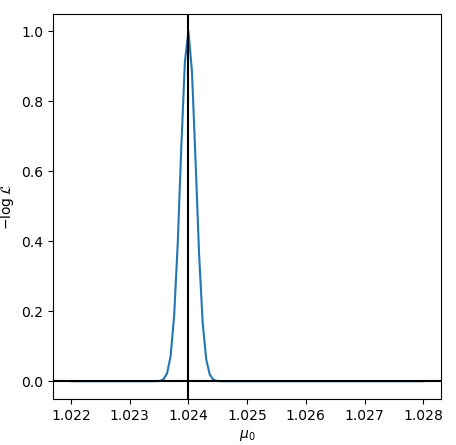
\includegraphics[width=\textwidth]{MainLayout/BORG_chapter/figures/muA_L.png}
        \caption{Likelihood profile for $\mu_A$}
        \label{fig:muA_lpt_L}
    \end{subfigure}
    \caption{Likelihood profiles of $\alpha$ and $\mu_A$ for a synthetic N-body simulation generated with LPT}
    \label{fig:params1_lpt_L}
\end{figure}

\begin{figure}
    \centering
    \begin{subfigure}{0.45\textwidth}
        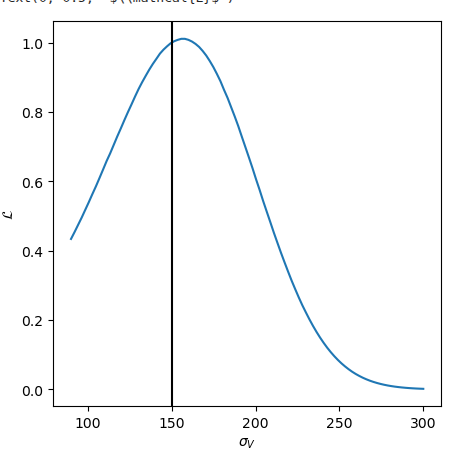
\includegraphics[width=\textwidth]{MainLayout/BORG_chapter/figures/sigma_v_L.png}
        \caption{Likelihood profile for $\sigma_v$}
        \label{fig:sigma_v_lpt_L}
    \end{subfigure}
    \hfill
    \begin{subfigure}{0.45\textwidth}
        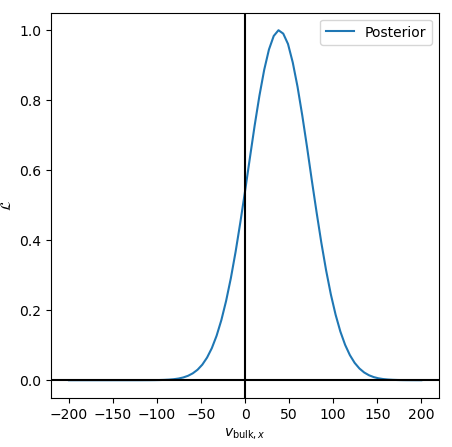
\includegraphics[width=\textwidth]{MainLayout/BORG_chapter/figures/bulk_x_L.png}
        \caption{Likelihood profile for $V_x$}
        \label{fig:Vx_lpt_L}
    \end{subfigure}
    \caption{Likelihood profiles $\sigma_v$ and $V_x$ for a synthetic N-body simulation generated with LPT}
    \label{fig:params2_lpt_L}
\end{figure}

\begin{figure}
    \centering
    \begin{subfigure}{0.45\textwidth}
        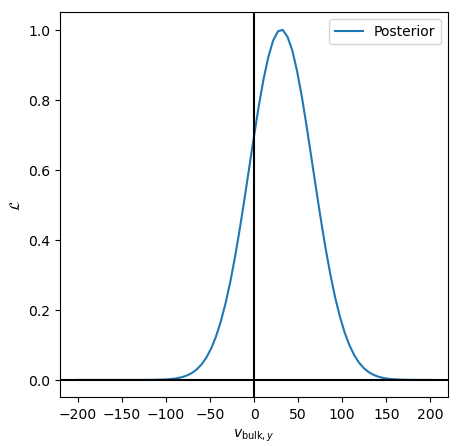
\includegraphics[width=\textwidth]{MainLayout/BORG_chapter/figures/bulk_y_L.png}
        \caption{Likelihood profile for $V_y$}
        \label{fig:Vy_lpt_L}
    \end{subfigure}
    \hfill
    \begin{subfigure}{0.45\textwidth}
        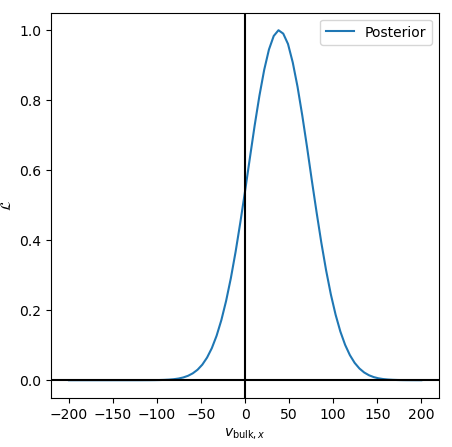
\includegraphics[width=\textwidth]{MainLayout/BORG_chapter/figures/bulk_x_L.png}
        \caption{Likelihood profile for $V_z$}
        \label{fig:Vz_lpt_L}
    \end{subfigure}
    \caption{Likelihood profiles $V_z$ and $V_z$ for a synthetic N-body simulation generated with LPT}
    \label{fig:params3_lpt_L}
\end{figure}

\subsection{Supernova prior improvement $-$ Towards a realistic description of supernovae}

Recent results from \cite{Lordet_2026} have shown that supernovae tend to be found in overly dense regions in the Universe with a large number of supernovae being present at a 
redshift of $z \approx 0.02-0.03$ creating what we see as a "bump" in the supernovae distribution accross redshift. This means that the assumption that the supernovae density is 
constant at low redshift (example of what was done in \cite{Perley_2020}) is not the most accurate description of the supernova distribution. We aimed at trying to account for such 
effects in our model description. We propose a slightly modified version of the supernova prior based on the observed supernova count. The number of supernova 
$N_{\text{SN}}$ observed by a survey between a distance $r$ and $r+dr$ can be expressed as:
\begin{equation}
    dN = n(r) \times 4 \pi r^2 dr
\end{equation}
where $n(r)$ is the number density of supernovae. This can be related to the observed rate as:
\begin{equation}
    R(r) = \mathrm{S}(\phi, \theta, r) \frac{n(r)}{T_{\text{obs}}}
\end{equation}
where $T_{\text{obs}}$ is the time of observation and $\mathrm{S}$ is a selection function that would account for the survey's footprint, galactic extinction and any 
instrumental effects that would decrease the number of observed supernova. Since we are working with the volume limited sample and are 
generating supernova on the full-sky $\mathrm{S}$ becomes unity. 
If we assume a constant rate, then $dN \propto r^2 dr$ giving the $r^2$ geometric dependence in the prior described earlier in Chapter 5 with the self consistent simulations. If we 
assume that this is not the case, then we get:
\begin{equation}
    dN(r) \propto n(r)r^2 dr
\end{equation}
In practice, we do not have direct access to $n(r)$ but we can infer $n(z)$. In Figure (ref) we show the $n(z)$ distribution obtained on the ZTF simulations obtained in 
100? bins up to a redshift of $z=0.06$. We proceed to then fit the number density with a cubic spline. The purpose of fitting with a cubic spline is to keep the $n(z)$ 
differentiable as it will be needed to then infer $n(r)$. In fact, we can relate the two number densities with:
\begin{equation}
    n(r) \propto \frac{n(z)}{4\pi r^2 \times \frac{dr}{dz}}
\end{equation}
The $\frac{dr}{dz}$ term can be deduced from Equation \ref{eqn:physical_distance} and is entirely determined by the cosmology. We get $\frac{dr}{dz} = \frac{c}{H(z)}$
Finally, we can present a more realistic prior on supernovae expressed as:
\begin{equation}
    p(r) \propto r^2\, n(r)\,(1+\delta^F)^{\alpha},
    \quad \text{with } n(r) \propto \frac{n(z)}{4\pi r^2 \times \frac{dr}{dz}}.
\end{equation}

*** We need to test this on both a constant rate simulation and a none constant rate ***
%\section{Results of the field level inference}

- results
 - covariance additions
 - full dataset with selection?

 \section{Comparison with other methods for $f\sigma_8$}
 can compare with results from Rafael


\chapter{Conclusion}
\section{General Conclusion}


Improving constraints on the growth rate of large-scale structures, 
$f\sigma_8$, is one of the central challenges of modern cosmology, as it 
provides a direct test of gravity on cosmological scales. During this 
PhD, I addressed this challenge along two complementary directions using 
Type Ia supernovae from the ZTF survey: improving the precision and 
characterization of supernova distance measurements, and developing a 
field-level inference approach to reconstruct the density and velocity 
fields of the nearby Universe. \\

The first direction focused on improving supernova distance measurements 
through the continued development and application of the NaCl framework, 
an algorithm designed to train empirical Type Ia supernova 
spectrophotometric models while simultaneously fitting their light 
curves. In its current implementation, the trained model adopts a 
SALT2-like parameterization consisting of two global spectral surfaces, 
$M_0(p,\lambda)$ and $M_1(p,\lambda)$, together with a color law, 
$CL(\lambda)$. 

After its initial development, NaCl required a substantial rewrite to 
make it suitable for \textsc{Lemaître}-scale datasets, and I contributed to this  
effort. Among the developments introduced during this rewrite, I 
extended NaCl to handle spectrophotometric data directly. In particular, 
the use of the SNfactory dataset required adapting the framework so that 
accurately flux-calibrated spectra could be modeled without introducing 
the spectral recalibration polynomial normally used for heterogeneous 
spectroscopic data. This also required reintroducing the color law in 
the spectral model and fitting the $X_0$ parameter of each supernova 
directly from its spectra. Applied to the SNfactory dataset, NaCl 
successfully trained a model on real spectrophotometric data and 
revealed some of the limitations of the SALT2 parameterization in 
describing supernova diversity, in particular in the UV and around the 
Si II and Ca II spectral features.

My work also included the development of an adaptive regularization 
scheme designed to strengthen the model constraints in regions of 
phase-wavelength space where the training data are sparse. This scheme 
is not currently part of the production version of NaCl, as its present 
implementation prevents the minimization from fully converging. Further 
work will therefore be required to stabilize the procedure, possibly 
through a reformulation of the regularization term. 

NaCl is also an essential component of the \textsc{Lemaître} project, which 
combines data from the ZTF, SNLS, and HSC surveys to construct an 
independent Hubble diagram containing approximately 3000 Type Ia 
supernovae over the redshift range $0<z<1.5$. The development of the new 
georges cosmological analysis pipeline within \textsc{Lemaître} required an 
extensive programme of validation on simulated datasets through a series 
of data challenges. The pre-DC1 and DC1 exercises presented in this 
thesis were used to validate the NaCl component and its propagation 
through the downstream analysis. 

These tests show that NaCl is able to reproduce the simulated 
photometric and spectroscopic observations accurately and to recover the 
supernova parameters and their covariance structure with good precision. 
The uncertainties inferred from the Fisher matrix are overall consistent 
with the empirical uncertainties measured across repeated realizations, 
although residual discrepancies remain for some parameters and require 
further investigation. 

However, once the complete NaCl-EDRIS-\texttt{cosmologix} chain is considered, 
significant biases are observed in the reconstructed distance moduli, 
particularly near the transitions between the different survey samples. 
These biases propagate into the inferred cosmological parameters. Their 
origin has not yet been conclusively identified and may involve model 
regularization, effective selection effects introduced by the analysis 
cuts, or limitations in the propagation of the covariance matrix. 
Resolving these effects is an essential step before the pipeline can be 
applied to the blinded \textsc{Lemaître} dataset. \\


The second front focused on applying the BORG Bayesian field-level inference pipeline on ZTF Type Ia supernovae. The goal of this is to obtain the most accurate reconstruction 
of the velocity field from the supernovae by directly inferring the initial conditions of the underlying matter field, and with the use of a gravity model, obtain the 
large scale structures. BORG has proven to be more accurate than other widely used methods in reconstructing the velocity field. With the development of a novel BORG-PV pipeline 
that includes an improved selection modeling and supernova prior, tests on self-consistent simulations have shown the capability of accurate reconstruction of the density and velocity 
fields. The pipeline has also proved capable in inferring cosmological parameters such as $\Omega_m$ and $\sigma_8$ under the assumption of $\Lambda$CDM. 
When applied to more realistic ZTF-like simulations generated from the 
Uchuu N-body simulation, the pipeline has proven to struggle in reconstructing the 
density and velocity fields. Further investigation has shown that may be due to model mismatches. 
These results motivate further investigation of the simulation framework and supernova modeling before applying the pipeline to real ZTF data.
These results pave the way for future analyses for the measurement of $f\sigma_8$ and for cross-survey analyses with galaxy clustering. 



\section{Future Prospects}

The work conducted during this PhD presents the base of a larger and more complete analysis of the ZTF Type Ia supernova data. On the side of NaCl, 
additional testing on capturing calibration uncertainties is needed within DC3 and a color scatter implementation is needed for DC4 before finalizing the NaCl 
framework.  
Moreover, a more complex 
error model needs to be implemented in order to capture uncertainties that are wavelength-phase-dependent as well as to spot outliers that may have 
contaminated the training dataset. 
Once that is complete, DC5 can be tested and the pipeline can operate on the full-blinded \textsc{Lemaître} dataset 
in order to obtain 
an independent measurement of the dark energy equation of state $w$ 
and its potential time variation $w_a$, with a dataset of $\sim 3000$ 
Type Ia supernovae spanning $0 < z < 1.5$. 
Running the full pipeline will also give us access to accurate measurement of the supernovae distances, which will then allow us to proceed with $f\sigma_8$ measurements. \\


On the BORG-PV side, more realistic ZTF simulations are needed in order to validate the pipeline. This includes applying masks to only cover the ZTF footprint 
as well as masking the Milky Way on the line of sight. 
An important aspect not yet accounted for is the correlation between 
supernova distance measurements, which were seen in Chapter \ref{chap4}. 
Accounting for these correlations within the BORG-PV likelihood is a challenge that must be met before operating on the ZTF data. 
Lastly, in order to operate on the full ZTF dataset, a more complex selection function is needed within the likelihood. 

Another aspect that can be explored within BORG-PV is the possibility of conducting a cross-survey analysis. 
One approach would be to use the Manticore-Local constrained realization 
of the local Universe as the density field for BORG-PV. 
This would enable a joint inference 
combining the velocity information from ZTF supernovae with the density 
field information from the galaxy survey, effectively performing a 
multi-tracer field-level inference. 
The exact incorporation of a multi-probe analysis is yet to be determined, and extensive testing on simulations is required before moving on to applications on real data. \\

The methods developed during this PhD lay the groundwork for future 
analyses with the Vera C. Rubin Observatory's LSST, which will provide 
an order of magnitude more Type Ia supernovae at low redshift, enabling 
tighter constraints on $f\sigma_8$ and a rigorous test of $\Lambda$CDM.





%


\urlstyle{same}


\newpage
\thispagestyle{empty}
\newgeometry{hmargin=2cm, vmargin=1.5cm}
\parskip 7pt

\selectlanguage{french}

{\bfseries Titre :}

Titre ici

{\bfseries Résumé} \Gray{(en français)} {\bfseries :}

----

{\bfseries Mots-clés :}

Supernova, galaxie

\vspace*{3mm}
\hrulefill
\vspace*{3mm}

\selectlanguage{english}

{\bfseries Title:}

Title here

{\bfseries Abstract} \Gray{(in english)}{\bfseries:}

-------

{\bfseries Keywords:}

Supernova, galaxy



\newgeometry{a4paper, right=2.5cm, left=2.5cm, top=3.cm, bottom=4.cm}
\bibliographystyle{apalike}
\raggedbottom
\bibliography{References}
\restoregeometry


\end{document}